\documentclass[reqno]{immbook}
%
\usepackage{amsmath}
\usepackage{amsfonts}
\usepackage{amssymb}
%
%
\usepackage{graphicx}
%\usepackage{makeidx}
%
\usepackage{mathptmx}
%
\newcommand{\Real}{\mathbb{R}}
%
\newcommand{\BA}{\vec{\textbf{a}}}
\newcommand{\BB}{\vec{\textbf{b}}}
\newcommand{\BE}{\vec{\textbf{e}}}
\newcommand{\BF}{\vec{\textbf{f}}}
\newcommand{\BG}{\vec{\textbf{g}}}
\newcommand{\BP}{\vec{\textbf{p}}}
\newcommand{\BQ}{\vec{\textbf{q}}}
\newcommand{\BU}{\vec{\textbf{u}}}
\newcommand{\BV}{\vec{\textbf{v}}}
\newcommand{\BW}{\vec{\textbf{w}}}
\newcommand{\BX}{\vec{\textbf{x}}}
\newcommand{\BY}{\vec{\textbf{y}}}
%
\newcommand{\BZero}{\vec{\textbf{0}}}  % Bold Zero (not "Z")
%
\newcommand{\T}{\rule{0pt}{2.6ex}}
\newcommand{\B}{\rule[-1.2ex]{0pt}{0pt}}
%
\newcommand{\ds}{\displaystyle}
%

%
\title{\fbox{\fbox{\fbox{\includegraphics{fig/IMMtitle.eps}}}}}
\author{Warren Weckesser\\
Department of Mathematics\\
Colgate University\\
\vspace{0.5in}
\centerline{%
\includegraphics[width=2in]{matlab/SIRscript.plot.eps}%
\hspace{0.4in}%
\includegraphics[width=1.6in]{matlab/LinPhPortExample1.eps}%
}
\vspace{0.1in}
\centerline{%
\includegraphics[width=2in]{matlab_map1d/logisticmap_timeseries.eps}%
\hspace{0.4in}%
\includegraphics[width=2in]{fig/trans_diag.eps}
}
\vspace{0.25in}
{\small Copyright \copyright ~2005, 2006 Warren Weckesser}}
%
\numberwithin{equation}{chapter}
\newtheorem{question}{Question}
\newtheorem{theorem}{Theorem}
\numberwithin{question}{section}
\numberwithin{theorem}{chapter}
\numberwithin{figure}{chapter}
%
\theoremstyle{definition}
\newtheorem{exercise}{}[section]
\newtheorem{example}{Example}[section]
\newtheorem{definition}{Definition}[section]
%
%
\newenvironment{xexample}%
{%

\medskip\noindent\addtocounter{example}{1}$\blacksquare$ \textsc{Example \theexample}\hspace*{1em}%
}%
{%
~\hfill$\square$

\medskip
}
%
%
\newenvironment{exercises}%
{%
\medskip\hrule\medskip\noindent\textbf{Exercises}%
}%
{%
\medskip\hrule
}
%
\makeindex
%
\begin{document}
\frontmatter
\maketitle
\tableofcontents
%
%
%%%%%%%%%%%%%%%%%%%%%%%%%%%%%%%%%%%%%%%%%%%%%%%%%%%%%%%%%%%
%

\chapter*{Foreword}
\textbf{Rough notes for now...}
\begin{itemize}
\item Goals: (i) Convert a description of a dynamical process
into a set of mathematical equations.
(ii) Use an appropriate combination of analysis and computer
simulation to study the mathematical model.
\item  I have intentionally minimized the
number of examples from physics.
One goal of this book is
to promote the use of mathematical models in fields outside of the
physical sciences.
\item The emphasis of the modeling is dynamic processes.
The mathematical topics are differential equations, discrete maps,
and Markov Chains (which are, in fact, linear maps).
Optimization, linear programming and other related topics
are \emph{not} covered in this book.
Another vital area of applied mathematics that is not
covered here is statistics.
\item Prerequisite for the book include calculus (single variable)
and basic linear algebra.  The essential facts from linear algebra that
are needed in this book are summarized in an appendix.
\item A brief introduction to probability is given in the
first section of the chapter on Markov chains. This section
can be skipped if the students have already had a course
on basic probability.
\end{itemize}
%
\mainmatter
%
%
%%%%%%%%%%%%%%%%%%%%%%%%%%%%%%%%%%%%%%%%%%%%%%%%%%%%%%%%%%%
%

\chapter{Introduction}
%
Love and marriage.  Battles and wars.
Drugs and disease. Fun and games.
These are \emph{not} the typical subjects that most
people think of when asked ``How is mathematics used
in the real world?''

...

This is a text on \emph{mathematical modeling}.
Actually, it is a bit narrower than that.
It is a text on modeling a selected class of
problems.  These are \emph{dynamic} problems;
problems in which \emph{time} (either continuous
or discrete) is the independent variable.

\bigskip
\noindent
\emph{``The merit of painting lies in the exactness of reproduction.
      Painting is a science and all sciences are based on mathematics. 
      No human inquiry can be a science unless it pursues its path
      through mathematical exposition and demonstration.''}

\hfill -- Leonardo Da Vinci

\bigskip
\noindent
\emph{``As far as the laws of mathematics refer to reality, they are not
certain, and as far as they are certain, they do not refer to reality.''}

\hfill  --Albert Einstein
\index{Einstein, Albert}

%
%%%%%%%%%%%%%%%%%%%%%%%%%%%%%%%%%%%%%%%%%%%%%%%%%%%%%%%%%%%
%
\newpage

\section{Modeling: An Introductory Example}

\subsection*{Classifying Mathematical Models -- An Example}
We consider the following scenario.
During a storm, a large tree with several
mice is blown into the ocean.  The storm carries the
tree many miles until it washes ashore on an
island that, until now, has had no mice.
This island has many seed-bearing plants that
mice love, and a nice climate, so the mice
have a good chance to survive and prosper.

How will the population of mice on this island
change over time?

For simplicity, we will consider just the population of female
mice.
We will also assume that a new generation is produced
each year.
We begin by making the following assumptions
\begin{enumerate}
\item In each generation, each female produces three offspring
(along with some number of males).
\item The offspring can reproduce after one year.
\item Mice live forever.
\end{enumerate}
Clearly these are not realistic assumptions.
We will accept them for now, in order to develop
a simple model.  Later we will look at some more
realistic variations.

To start, we will work with
\emph{discrete time}.
Let $p(n)$ be the population at the end of the
$n$th year, where $n$ is an integer.
With this notation, $p(0)$ is the initial population.
Let's suppose that $p(0)=1$; that is, the initial
population contained just one female mouse.

At the end of the first year, this mouse has produced
three female offspring,
so $p(1) = 4$.  At the end of the second year,
each of the four mice has produced three more offspring,
so $p(2) = 16$.
In general, we have
\begin{equation}
   p(n+1) = 4p(n)
\label{eqn:mousepop}
\end{equation}
Equation \eqref{eqn:mousepop} is the rule that describes
how the population changes over time.  Such a rule
involving discrete time is sometimes called 
a \emph{difference equation}.
\index{difference equation}
This terminology is a bit clearer if we rewrite the
equation as
\begin{equation}
    p(n+1)-p(n) = 3p(n)
\label{eqn:mousepopdiff}
\end{equation}
This gives the rule for computing the difference
between successive generations.

We can easily verify that \eqref{eqn:mousepop}
has the solution
\begin{equation}
   p(n) = p(0)4^n
\label{eqn:mousepopsol}
\end{equation}
This is a solution in the sense that the 
population at time $n$ is given directly
as a function of $n$ and the initial
population.

If we plot this solution, we will see
a ``stair-step'' plot, with the size of
the steps getting larger as $n$ increases.
If all the mice produce their offspring
at exactly the same time, then this stair-step
shape is reasonable. But we don't really expect
that to be the case.  Presumably mice will
be born throughout the year, and we expect the
actual graph of the population to have many smaller steps.
In fact, when the
population is large (and if we blur our vision
a bit), we might expect the graph to look like
a smooth curve.
Let $p(t)$ be the population at time $t$, where
now $t$ is a real number.
What mathematical
rule is obeyed by $p(t)$?


If we still believe our assumptions,
we still expect that in one year, the population
increases four-fold.
That is, we still have
\begin{equation}
    p(t+1) = 4p(t)
\label{eqn:mousepopcont}
\end{equation}
What is the corresponding rule for increments of
time less than one year? That is, what can we
say about $p(t+\frac{1}{2})$, $p(t+\frac{1}{3})$,
or in general, $p(t+h)$?
I claim that the correct rule is
\begin{equation}
   p(t+h) = 4^{h}p(t)
\label{eqn:mousepoph}
\end{equation}
If $h=0$, we obtain $p(t)=p(t)$, as we should, and if
$h=1$, we obtain \eqref{eqn:mousepopcont}.
If $h=1/k$, where $k$ is an integer, we have
\begin{equation}
\begin{split}
   p(t+1) & = p(t+\frac{k-1}{k} + \frac{1}{k}) \\
          & = 4^{1/k}p(t+\frac{k-1}{k}) \\
	  & = 4^{2/k}p(t+\frac{k-2}{k}) \\
	  & \quad \vdots \\
	  & = 4^{\frac{k-1}{k}}p(t+\frac{1}{k}) \\
	  & = 4p(t)
\end{split}
\end{equation}
so the repeated application of \eqref{eqn:mousepoph}
with $h=1/k$ also agrees with \eqref{eqn:mousepopcont}.

We now subtract $p(t)$ from both sides of
\eqref{eqn:mousepoph}, and divide by $h$:
\begin{equation}
   \frac{p(t+h) - p(t)}{h} =
     \frac{4^{h} p(t) - p(t)}{h} = \left(\frac{4^h-1}{h}\right)p(t).
\end{equation}
Take the limit $h\rightarrow 0$.
On the left we obtain $p'(t)$.
On the right, we apply L'Hopital's Rule
(and recall that $\frac{d}{dx}\left[a^x\right] = \ln(a)a^x$)
to obtain $\ln(4)p(t)$.
Thus we have
\begin{equation}
   p'(t) = \ln(4)p(t)
\label{eqn:mousepopdiffeq}
\end{equation}
This is a \emph{differential equation}.
\index{differential equation}
This equation says that the
instantaneous rate of change of the population
at time $t$ is proportional to the population at time $t$;
the proportionality constant is $\ln(4)$.

Equations \eqref{eqn:mousepop} and
\eqref{eqn:mousepopdiffeq} both give rules
for determining the population.
The first is a \emph{discrete time} model,
and the second is a \emph{continuous time}
model.
This distinction is one of the fundamental
categorizations of models.

We now consider a more complicated discrete model, 
in which we no longer assume that the mice live forever.
Suppose the mice only live three years.
Moreover, each female mouse produces two female
offspring during its second year and its third year.
At time $n$, we need \emph{three}
quantities to describe the state of the population.
We define
\begin{itemize}
\item $p_0(n)$ is the number of new female offspring
in year $n$;
\item $p_1(n)$ is the number of one-year-old females in year $n$; and
\item $p_2(n)$ is the number of two-year-old females in year $n$. 
\end{itemize}
Then we have
\begin{equation}
\begin{split}
   p_0(n+1) & = 2p_1(n) + 2p_2(n) \\
   p_1(n+1) & = p_0(n) \\
   p_2(n+1) & = p_1(n)
\end{split}
\label{eqn:mouseagemodel}
\end{equation}
Suppose that in the initial population,
$p_0(0)=0$, $p_1(0)=2$ and $p_2(0)=0$.
Let's compute the population for a few generations:

\centerline{%
\begin{tabular}{ccccc}
%   MM \= MMM \= MMM \= MMM \= MMMM \kill
   $n$ & $p_0(n)$ & $p_1(n)$ & $p_2(n)$ & Total \\
    0  &   0      &   2      &    0     &   2 \\
    1  &   4      &   0      &    2     &   6 \\
    2  &   4      &   4      &    0     &   8 \\
    3  &   8      &   4      &    4     &   16 \\
    4  &   16     &   8      &    4     &   28
\end{tabular}
}

We appear to have a growing population, but unlike
the simpler model, a formula for the solution
is not obvious.  (We will see how to solve a problem
like this later in the course.)

A key observation to make about the model
is that the ``state'' of the population
is three dimensional. In order to write down the rules
that determine how
the population changes, we needed to keep track
of three quantities.  We can put these in a vector:
\begin{equation}
   \BX(n) = \begin{bmatrix} p_0(n) \\ p_1(n) \\ p_2(n)
            \end{bmatrix}
\end{equation}
Then the rules given in
\eqref{eqn:mouseagemodel} can be written
more concisely as
\begin{equation}
   \BX(n+1) = \BF(\BX(n))
\label{eqn:general_map}
\end{equation}
where $\BF$ is the vector-valued function
(or \emph{map}, or \emph{mapping})
\index{map, mapping}
given by the right side of \eqref{eqn:mouseagemodel}.

Equation \eqref{eqn:general_map}
is a general form for multi-dimensional
discrete time models.
We will often call such an equation an
\emph{iterated map}.
\index{iterated map}
 (Just like the one-dimensional
case, these are also often called \emph{difference equations}.)
\index{difference equation}

We will also study multi-dimensional
\emph{systems of differential equations}:
\index{differential equation, system}
\begin{equation}
   \BX'(t) = \BF(\BX(t))
\label{eqn:general_diffeq}
\end{equation}
where
\begin{equation}
   \BX(t) = \begin{bmatrix}x_1(t) \\ x_2(t) \\ \vdots \\ x_m(t)\end{bmatrix}
   \quad
   \textrm{and}
   \quad
   \BX'(t) = \begin{bmatrix}x_1'(t) \\ x_2'(t) \\ \vdots \\ x_m'(t)\end{bmatrix}
\end{equation}

\subsection*{Deterministic vs. Stochastic Models.}
We have one more important categorization to discuss.
Both \eqref{eqn:general_map} and \eqref{eqn:general_diffeq}
are \emph{deterministic}.\index{deterministic}
That is, for a given starting state (e.g. $\BX(0)$),
the fate of the population is determined;
the equations produce only one possible solution.
There are no random events incorporated in the model.

Models that explicitly include random events are 
called \emph{stochastic}.\index{stochastic}
For example, suppose we model a population of mice
with the rule that in each year, there is a one in ten
chance that a mouse will die, and a one in two chance that
the mouse will produce one offspring.
(This means there is a four in ten chance that the mouse
will not die and will not produce an offspring.)
In such a model, if the initial population is 1, then
in the next year the population could be 0, 1, or 2.
The following year it could be 0, 1, 2, 3 or 4.
Figure \ref{fig:StochModel} shows five instances of
the population for this model. In all five cases,
the initial population is 2.

\begin{figure}
\centerline{\includegraphics[width=3.5in]{matlab/StochModel.eps}}
\caption{Five instances of the population in 
a stochastic model.}
\label{fig:StochModel}
\end{figure}

In such models, the question that we ask is not
``What is the population in year $n$?''
Rather, we usually ask ``What is the probability
distribution of the population in year $n$?''
If we have the probability distribution at year
$n$, we can then answer questions such as
``What is the probability that the population is zero?''
or ``What is the probability that the population is
greater than 500 in year 10?''

Figure \ref{fig:StochDist} shows a numerically
computed distribution of the population after
five years. This was computed by running 50000
simulations, and adding up the number of times
each possible final population occurred.
For example, in the figure we see that
approximately 3.6\% of the time, the population
is zero after five years.

\begin{figure}
\centerline{\includegraphics[width=3.5in]{matlab/StochDist.eps}}
\caption{Numerically computed population
probability distribution for the population
after five years.  This was computed by
tallying the results of 50000 individual
simulations.}
\label{fig:StochDist}
\end{figure}


\chapter{Differential Equations}
\index{differential equation}


% \section{Modeling with Differential Equations}
% \emph{Start with an example; discuss significance of a
% relationship between and function and its derivative...}
% %
% The general form of a first order (autonomous) differential
% equation is
% \[
%    \frac{dy}{dt} = f(y)
% \]
% \noindent
% If  $f'(y_{0})=0$, then $y(t)=y_{0}$ is a solution.  Such a constant
% solution is called an \emph{equilibrium solution}.\index{equilibrium}

\section{Unconstrained Population Growth}
\label{sec:UnconstrPopGrowth}
% \noindent
% \emph{``Population, when unchecked, increases in a geometrical ratio. 
%       Subsistence increases only in an arithmetical ratio."}
% 
% \hfill    -- Thomas Robert Malthus
% 
% \bigskip
The simplest assumption for modeling the growth of a population
with a continuous time model is
\begin{quote}
\emph{The rate of change of the population is proportional to the current population level.}
\end{quote} 
Let $t$ be time, and let $p(t)$ be the population at time $t$.
For now we'll assume that some convenient system of units is used;
we'll have more to say about units later.
We also assume that $p$ is ``large'' in some sense, so that it is reasonable
to treat $p$ as a real number, not an integer.
If, for example, the population was just three rabbits, the following
models would not provide good
approximations to the actual growth of the population.
If the population is measured in thousands of rabbits,
then $p(0)=3.12$ makes sense,
and the following models are more reasonable.

We convert the above assumption into an equation involving $t$
and $p$.
The ``rate of change of the population'' is the derivative, $\frac{dp}{dt}$, and the
current population is $p(t)$, so the mathematical version of the above
assumption is
\begin{equation}
  \frac{dp}{dt} = rp
\label{eqn:growth}
\end{equation}
where $r$ is the constant of proportionality.
(Note that I have suppressed the argument of $p$ for brevity.)
This is a \emph{first order differential equation}.
(The \emph{order}\index{order} of a differential equation is the order of the
highest derivative in the equation.)

Frequently, the question we ask is ``What is the population at time $t$
if the population is $P_0$ at time $t=0$?''  That is, we impose the
condition that $p(0)=P_0$.  This is called an
\emph{initial condition}, and the problem of solving the differential
equation with a given initial condition is called an
\emph{initial value problem}.

To solve this equation, we must find a \emph{function} $p(t)$
that satisfies the equation.  In this case, the solution\footnote{%
``Who has not been amazed to learn that the function $y = e^x$, like a 
      phoenix rising from its own ashes, is its own derivative?'' 
       -- Francois le Lionnais
}
is
\begin{equation}
  p(t) = P_0 e^{rt}
\end{equation}
(Let's check:  $\frac{dp}{dt} = rP_0e^{rt} = r p(t)$, so  it solves the differential
equation, and $p(0) = P_0e^0 = P_0$, so it also satisfies the initial condition.)
Thus, if $r > 0$, the simple assumption given above results in
\emph{exponential growth}.\index{exponential growth}
(If $r < 0$, we obtain \emph{exponential decay}.\index{exponential decay})

\newpage

\begin{exercises}
\begin{exercise}
\label{ex:UnconstrPopGrowth_halflife_formula}
When the number of atoms in a radioactive sample is large,
the following statement is found to be accurate:
\emph{The amount of the radioactive isotope decays at 
a rate that is proportional to the amount present.}
Let $y(t)$ be the amount of the isotope at time $t$.
The differential equation for $y$ is generally written
\[
   y'(t) = -ry
\]
where we assume $r > 0$.  The solution is
\[
   y(t) = y_0 e^{-rt}.
\]
The \emph{half-life}\index{half-life} $h$ of a radioactive
isotope is the time required for the amount to be reduced
to half the original amount.
Use the above formula to express $r$ in terms of $h$.
\end{exercise}
\begin{exercise}
\label{ex:UnconstrPopGrowth_americium}
The radioactive element americium-241 has a half-life
of 458 years.
If a sample initially contains 3 mg of americium-241,
find the amount of americium-241 that remains
after (a) 10 years, (b) 916 years, (c) 10000 years.
\end{exercise}
\begin{exercise}
\label{ex:NewtonsLawOfCooling}
\emph{Newton's Law of Cooling}\index{Newton's Law of Cooling}
says that the rate of change
of the temperature of an object is proportional
to the difference between the temperature of the object
and the ambient temperature of the air.

Express this statement as a differential equation.
Use $k>0$ for the proportionality constant, and define
\emph{with complete sentences}
any other variables or constants that you use in the equation.

\end{exercise}
\end{exercises}

\newpage

\section{The Logistic Equation\index{logistic equation}}

For a population with unlimited resources, exponential growth
is a pretty accurate description of what happens.
However, no environment can support exponential growth forever.
Eventually the food runs out, or there is simply not enough space
for a larger population.
Presumably there is a maximum population level that the environment
can sustain.  This level is called the
\emph{carrying capacity}\index{carrying capacity}
of the environment. If the population is larger than the
carrying capacity, overcrowding or a lack of food results in a
\emph{decreasing} population.
We'll modify the growth equation
\eqref{eqn:growth} to take this into account.

The right side of the equation gives the rate of change of $p$
as a function of $p$.
If we divide the the right side by $p$, we obtain the
\emph{per capita growth rate},
\index{growth rate, per capita}
For the initial assumption,
the per capita growth rate  is just the constant $r$.
To incorporate the assumption of a carrying capacity, we will assume that the
per capita growth rate depends on $p$.
When $p$ is near zero, we assume that there
are plenty of resources for the population to grow, so the
per capita growth rate should be
near $r$.  As the population becomes bigger, the per capita growth rate
should decrease: with fewer resources available to each individual,
we assume that the reproductive ability of each individual decreases.
The per capita growth rate
should be zero when the population is at the carrying capacity.
If the population exceeds the carrying capacity, the growth rate should
be negative. In this case, conditions are so bad that the death rate
exceeds the birth rate.

The simplest formula for such a
per capita growth rate is a straight line that has
the value $r$ when $p=0$ and the value $0$ when $p=K$, as shown in
Figure~\ref{fig:growthrate}.
\begin{figure}
\centerline{\includegraphics[width=2.25in]{matlab/logistic_percapita_growthrate.eps}} 
\caption{Per capita growth rate for the logistic equation.}
\label{fig:growthrate}
\end{figure} 
The equation that we obtain is
\begin{equation}
  \frac{dp}{dt} = r\left(1-\frac{p}{K}\right)p
\label{eqn:logistic}
\end{equation}
This first order differential equation is commonly called the \emph{logistic equation}.\index{logistic equation}
(It is also known as the
\emph{Verhulst equation}.\index{Verhulst equation})
Later we'll see how to find the exact solutions to this equation.
For now, we'll learn as much as we can about its solutions without actually solving the
equation.  To do this, we plot the right side of \eqref{eqn:logistic} as a function of $p$.
The graph is shown in Figure~\ref{fig:logisticrhs}.
\begin{figure}
\centerline{\includegraphics[width=2.25in]{matlab/logistic_growthrate.eps}} 
\caption{A plot of $\frac{dp}{dt}$ as a function of $p$ for the logistic
equation \eqref{eqn:logistic}.}
\label{fig:logisticrhs}
\end{figure}
We can use the information in Figure~\ref{fig:logisticrhs} to determine the
behavior of solutions to \eqref{eqn:logistic}.
Suppose, for example, that the population is initially ``small''.
(In this case, small means ``a small fraction of $K$''.)
Then the graph in Figure~\ref{fig:logisticrhs} tells us that
$\frac{dp}{dt}$ is also small but positive.  In other words, the slope
of $p(t)$ is small and positive.  This means that $p(t)$ is an increasing
function of $t$, so in a little while, $p$ will be larger.  Looking back to
Figure~\ref{fig:logisticrhs}, we see that this means $\frac{dp}{dt}$ will be
larger than it was before, and therefore the slope of $p(t)$ has increased.
So initially, $p(t)$ will grow faster and faster.  This is not surprising, since
when $p$ is small, $p^2$ is very small, and if we ignore the $p^2$ term in the
logistic equation, we obtain $\frac{dp}{dt} \approx rp$.  So when the
population is small, the growth is almost exponential.

Eventually the population will reach $K/2$.  This is the population
level at which the population grows the fastest.
When the population reaches this level, further increases in the
population result in \emph{lower} growth rates.
If $K/2 < p(t) < K$, we see in
Figure~\ref{fig:logisticrhs} that $\frac{dp}{dt}$ is positive, but it is
decreasing as $p$ increases.  In the next moment, $p$ will be larger,
but then the slope of $p(t)$ will be smaller.
As $p$ gets closer to $K$, the slope gets smaller.
In fact, $p(t)$ will approach $K$ asymptotically, but never reach it.
A graph of a solution to the logistic equation~\eqref{eqn:logistic} is
shown in Figure~\ref{fig:logisticsol}.
\begin{figure}
\centerline{\includegraphics[width=2.25in]{matlab/logistic_solution.eps}} 
\caption{The graph of $p(t)$, a solution to the logistic
equation \eqref{eqn:logistic}.}
\label{fig:logisticsol}
\end{figure}


Note that if the initial population is exactly $K$, then
$\frac{dp}{dt} = 0$.  The constant function $p(t)=K$ is an
exact solution to the differential equation.
We call a constant solution an
\emph{equilibrium solution}.\index{equilibrium solution}

\newpage

\begin{exercises}
\begin{exercise}
Does the logistic equation \eqref{eqn:logistic} have any other
equilibrium solutions?
\end{exercise}
\begin{exercise}
Describe (and sketch) the solution that
results when the initial population is greater than $K$.
Use Figure \ref{fig:logisticrhs} to explain your answer.
Is the solution $p(t)$ increasing or decreasing?
Is the graph of $p(t)$ concave up or concave down?
What happens to $p(t)$ as $t\rightarrow\infty$?
\end{exercise}
\begin{exercise}
Find a formula for the maximum rate of change
of $p(t)$ if $0 < p(t) < K$.
\end{exercise}
\end{exercises}

\newpage

\section{Autonomous First Order Differential Equations}
The method for analyzing solutions to the logistic equation can be
applied to any first order equation of the form
\begin{equation}
   \frac{dy}{dt} = f(y)
\end{equation}
where $f(y)$ is a given function.
In particular, we assume that $t$ does \emph{not} appear explicitly
in $f$.  Such an equation is called \emph{autonomous}.\index{autonomous}
When $t$ appears explicitly in the right side of the equation,
we say the equation is \emph{nonautonomous}.\index{nonautonomous}
For example, the equation
\begin{equation}
  \frac{dp}{dt} = (r+a \sin(\omega t))p
\end{equation}
is nonautonomous, since $t$ appears explicitly in the right side of the
equation (in the argument of the sine function).
In this case, the explicit time dependence might model a growth
rate with seasonal dependence.

The basic procedure to analyze an autonomous
first order differential equation is to sketch the graph of $f(y)$, identify
the equilibrium solutions (where $f(y)=0$), and determine the
behavior of non-equilibrium solutions based on the graph
of $f(y)$.

\begin{xexample}
Consider the equation
\begin{equation}
\frac{dp}{dt} = -rp + b.
\label{eqn:auton_example}
\end{equation}
Suppose $r > 0$ and $b > 0$.
Then the graph of the right side of the equation looks like
the left plot in Figure~\ref{fig:auton_example_plots}.
\begin{figure}
\centerline{\includegraphics[width=1.75in]{matlab/auton_example_rhsplot.eps}\hspace{0.25in}\includegraphics[width=1.75in]{matlab/auton_example_solplot.eps}}
\caption{The left plot shows the graph of the right side of \eqref{eqn:auton_example}.
The right plot shows an example of a solution.}
\label{fig:auton_example_plots}
\end{figure}
Since $\frac{dp}{dt} = 0$ when $p = b/r$, we have an
equilibrium solution $p(t) = b/r$.

For $p < b/r$, $\frac{dp}{dt} > 0$, and for
$p > b/r$, $\frac{dp}{dt} < 0$.
So if $p(t) < b/r$, $p(t)$ is an increasing function of
$t$.  As $p$ increases, $\frac{dp}{dt}$ decreases; the closer
$p$ is to $b/r$, the closer $\frac{dp}{dt}$
is to zero.
This suggests that $p(t)$ will approach $b/r$ asymptotically
from below as $t\rightarrow\infty$.
A similar argument shows that if $p(t) > b/r$,
$p(t)$ will approach $b/r$ asymptotically from above.

The plot on the right in Figure~\ref{fig:auton_example_plots}
shows an example of a solution, for which $0 < p(0) < b/r$.
\end{xexample}

\newpage

\begin{exercises}
\begin{exercise}
\label{ex:AutFirstOrder_autclassify}
Classify each of the following first order differential equations
as autonomous or nonautonomous.

\medskip
\begin{tabbing}
\hspace*{0.25in} \= \hspace*{1.5in} \= \hspace*{1.5in} \= \kill
~ \> 
(a) $\ds \frac{dy}{dt} = y - y^3$ \>
(b) $\ds \frac{dx}{dt} = x\cos(t)$ \>
(c) $\ds \frac{dy}{dt} = 3t$ \\[2pt]
~ \>
(d) $\ds y'(t) = 3y(t) + t^2$ \>
(e) $\ds q'(t) = q(t) + 1$ \>
(f) $\ds \frac{dy}{dt} = \frac{\pi y}{y^2+1}$
\end{tabbing}
\end{exercise}
\begin{exercise}
Consider the differential equation
\[
   \frac{dy}{dt} = y(y-1)(y-2)
\]
\begin{enumerate}
\item[(a)] Find the equilibrium solutions.\\
\item[(b)] Sketch $\frac{dy}{dt}$ as a function of $y$.\\
\item[(c)] In one set of axes, sketch several solutions $y(t)$. Include the equilibrium solutions,
and several more non-equilibrium solutions to show all the possible behaviors.
(Since this is not necessarily a population model, you should consider negative values
of $y$ as well as positive.)
\end{enumerate}
\end{exercise}
\begin{exercise}
\label{ex:AutonomousDegreeThree}
Consider the first order autonomous differential equation
\[
   \frac{dy}{dt} = (y-2)(y^2+6y+8).
\]
\begin{enumerate}
\item[(a)] Find the equilibrium solutions, 
sketch the graph  of the right side of the equation as a function
of $y$, and use this graph to sketch the ``phase line''
(i.e. on the $y$ axis, add arrows between the equilibria
that indicate whether $y(t)$ is increasing or decreasing).
\item[(b)] In one set of axes, sketch several solutions ($y(t)$ vs. $t$), including
all equilibrium solutions.
(Other than the equilibria,
you do not have to find the solutions analytically.)
Be careful with your sketch and check that:
curves that should not cross do not
cross; curves that should be increasing functions of $t$
are increasing; and curves that should be decreasing functions
of $t$ are decreasing. Label the axes appropriately.
\item[(c)] If $y(0) = 1$, determine $\ds \lim_{t \rightarrow \infty} y(t)$
and $\ds \lim_{t\rightarrow -\infty} y(t)$.
\end{enumerate}
\end{exercise}
\begin{exercise}
For each of the following differential equations
of the form $y' = f(y)$,
determine the equilibrium solutions, sketch $f(y)$ as a function
of $y$, and sketch the solutions where $y(0)=1/2$, $y(0)=1$, and
$y(0)=3/2$.
\begin{tabbing}
\hspace*{0.25in} \= \hspace*{1.75in} \= \hspace*{1.5in} \= \kill
~ \> 
(a) $\ds y' = -2y + 1$ \>
(b) $\ds y' = y(2-y)$ \>
(c) $\ds y' = \sin(\pi y)$ \\[2pt]
~ \>
(d) $\ds y' = y^{1/2} - y$ ~~ $(y \ge 0)$ \>
(e) $\ds y' = (y-1)^2$ \>
(f) $\ds y' = (y-1)^3$
\end{tabbing}
\end{exercise}
% \begin{exercise}
% \emph{...a question in which a description must be converted to
% a differential equation...}
% \end{exercise}
% \begin{exercise}
% \emph{...another...}
% \end{exercise}
\end{exercises}

\newpage

\section{Separable First Order Differential Equations (*)}

In this section and the next, we discuss
two techniques for solving certain first order
differential equations.
The general form for a first order differential equation is
\begin{equation}
   y'(t) = f(t,y)
\end{equation}
In this section we discuss \emph{separable} equations,
and in the next we discuss \emph{linear} equations.

\medskip
If $f$ can be ``separated'' into a quotient of a function of $t$ and a function
of $y$ as
\begin{equation}
   f(t,y) = \frac{h(t)}{g(y)},
\end{equation}
there is a chance that the solutions can
be found analytically.
The differential equation may be written
\begin{equation}
  g(y(t))y'(t) = h(t).
\label{eqn:separated}
\end{equation}
(I have chosen to \emph{not} suppress the $t$ dependence of
$y$ for the moment.)
We now integrate both sides:
\begin{equation}
    \int_0^t g(y(s))y'(s) \, ds = \int_0^t h(s) \, ds
\label{eqn:integrated}
\end{equation}
The right side is an integral of a known function.
To deal with the left side, we first let $p(y) = \int_{y_0}^y g(z) dz$.
Then  we use the chain rule:
\begin{equation}
   \frac{d}{dt} p(y(t)) = p'(y)y'(t) = g(y)y'(t).
\end{equation}
Thus, on the left side of \eqref{eqn:integrated}, we have
\begin{equation}
  \int_0^t g(y)y'(s)\,ds = \int_0^t \left(\frac{d}{ds} p(y(s))\right)\, ds = p(y(t)) = 
    \int_{y_0}^y g(z) \, dz
\end{equation}
This means we can try to solve an equation of the form
\begin{equation}
   \frac{dy}{dt} = \frac{h(t)}{g(y)}
\end{equation}
with the following formal procedure:
\begin{enumerate}
\item Treat the derivative $\frac{dy}{dt}$ as a fraction and rewrite the differential equation
as
\begin{equation}
   g(y)dy = h(t)dt.
\end{equation}
\item Integrate with respect to $y$ on the left and with respect to $t$ on the right.
The constants of integration can be combined into one constant on the right after
integrating.
\item Solve for $y$.
\end{enumerate}
The \emph{real} short summary is:
\begin{quote}
  \emph{Separate}, \emph{Integrate}, \emph{Isolate} (i.e. solve for $y$).
\end{quote}
Note that even if $f$ can be separated into $h(t)/g(y)$, there are two potential obstacles
to this method. First, it might not be possible to evaluate the integrals.
Second, it might not be possible to solve for $y$ after integrating.
In this case, we have an implicit equation relating $y$ and $t$, which can still
be useful in some cases.

Note that all autonomous first order differential equations are separable.

\begin{xexample}
We'll apply the method to
\begin{equation}
   \frac{dp}{dt} = r p
\end{equation}
In this case, separating gives
\begin{equation}
   \frac{dp}{p} = r dt,
\end{equation}
but note that we have assumed that $p\ne 0$.
Integrating gives
\begin{equation}
   \ln | p | = rt+C_0
\end{equation}
Exponentiate both sides to obtain
\begin{equation}
  |p| = e^{rt+C_0} = C_1e^{rt}, \quad \textrm{where} \quad C_1 = e^{C_0}.
\end{equation}
Note that $C_1 > 0$.
For $p > 0$, we have $|p|=p$, so $p=C_1e^{rt}$.
If $p < 0$, $|p| = -p$, so $p = -C_1e^{rt}$.
This is the same as saying the constant in front of $e^{rt}$ is negative.
Also note that $p(t)=0$ is an equilibrium solution.
We can combine the three cases $p>0$, $p=0$ and $p<0$ into one
solution
\begin{equation}
   p(t) = Ce^{rt},
\end{equation}
where $C$ is an arbitrary constant.
To satisfy the initial condition $p(0)=P_0$, we let $C=P_0$.
\end{xexample}

\begin{xexample}
Now consider a population model in which the per capita growth
rate varies periodically, perhaps because of seasonal variation.
The differential equation is
\begin{equation}
   \frac{dp}{dt} = (r + a\cos(\omega t))p
\end{equation}
Separating gives
\begin{equation}
  \frac{dp}{p} = \left( r+a\cos(\omega t) \right) dt
\end{equation}
and integrating gives
\begin{equation}
  \ln | p | = rt + \frac{a}{\omega} \sin(\omega t) + C_0
\end{equation}
From here, the work is similar to the previous example.
The final concise formula for the solution is
\begin{equation}
   p(t) = Ce^{rt + (a/\omega)\sin(\omega t)}
\end{equation}
where $C$ is an arbitrary constant.
\end{xexample}
%
\begin{exercises}
\begin{exercise}
Solve the initial value problems.
\begin{enumerate}
\item[(a)] $\ds y' = -y/(t^2+1)$, \hspace{0.25cm} $y(0)=5$.
\item[(b)] $\ds y' = -\left(2-e^{-t}\right)y$, \hspace{0.25cm} $y(0)=3$.
\item[(c)] $\ds y' = (t+1)y^2$, \hspace{0.25cm} $y(0)=y_0$, where $y_0$ is
a constant.
\item[(d)] $\ds y' = e^{-rt}y$, ~~ $(r > 0)$, \hspace{0.25cm}
                                       $y(0)=1$.
\end{enumerate}
\end{exercise}
\begin{exercise}
\label{ex:SolveFirstOrderYCubed}
Solve the following initial value problem.
\[
  \frac{dy}{dt} = y^3, \quad y(0)=-2.
\]
\end{exercise}
\end{exercises}
%

\newpage

\section{Linear First Order Differential Equations (*)}
\label{sec:LinearFirstOrder}
If the first order differential equation has the form
\begin{equation}
    y'(t) = p(t) y + g(t),
\label{eqn:linear}
\end{equation}
it is called a \emph{linear} equation.
We can always express the solution to such an equation
in terms of integrals.  The only obstacle will be
evaluating the integrals.

To derive the solution, we first move $p(t)y$ to the left:
\begin{equation}
    y'(t) - p(t) y =  g(t),
\label{eqn:intermediateA}
\end{equation}
The left side looks vaguely like the result of applying the
product rule of differentiation to a product of $y$ and something else.
If $\mu(t)$ is some function, then $(\mu y)' = \mu y' + \mu' y$,
which suggests that we multiply \eqref{eqn:intermediateA}
by $\mu$ (whatever it is)
to obtain
\begin{equation}
    \mu y'(t) - \mu p(t) y =  \mu g(t),
\label{eqn:intermediateB}
\end{equation}
and then determine what $\mu(t)$ should
be by solving $\mu' = -\mu p(t)$.
This is a separable equation; a solution is
\begin{equation}
   \mu(t) = e^{-\int p(t)\, dt}.
\end{equation}
We could include an arbitrary multiple of this function
by multiplying it by an arbitrary constant $C$, but
since \emph{any} such $\mu(t)$ will work for us, we
might as well choose $C=1$.
(Equivalently, when we find the integral
$\int p(t)\,dt$, we choose the constant of integration
to be zero.)

With this choice of $\mu$, 
\eqref{eqn:intermediateB} becomes
\begin{equation}
    (\mu y)' =  \mu g(t).
\label{eqn:intermediateC}
\end{equation}
Integrating both sides gives%
\footnote{Note that I have explicitly included the integration
constant $C$ on the right.  Normally, when we write an indefinite
integral $\int q(t)\, dt$, the constant of integration is implicitly
assumed to be part of the result. For example, $\int 2x\,dx = x^2+C$.
However, it is a common mistake to \emph{forget} the constant, so
I choose to include it explicitly.}
\begin{equation}
    \mu y =  \int \mu g(t) \, dt + C
\label{eqn:intermediateD}
\end{equation}
and so we have the following solution
to \eqref{eqn:linear}:
\begin{equation}
    y =  \frac{1}{\mu}\left(\int \mu g(t) \, dt + C\right)
    \quad \textrm{where} \quad
    \mu(t) = e^{-\int p(t)\, dt}.
\label{eqn:linearsolution}
\end{equation}

\begin{xexample}
Consider the initial value problem
\begin{equation}
   y' = 2y + 3, \quad y(0) = 5.
\label{eqn:linearexample1}
\end{equation}
This problem is linear, with $p(t)=2$ and $g(t) = 3$.
(It is also separable, so there is more than one way
to solve this problem.)
The integrating factor is
\begin{equation}
   \mu(t) = e^{-\int p(t)\,dt} = e^{-\int 2\, dt}
      = e^{-2t},
\end{equation}
and the solution is
\begin{equation}
\begin{split}
   y(t) & = e^{2t} \left( \int \left(e^{-2t}\right)\left(3\right)\,dt + C\right) \\
        & = e^{2t} \left( -\frac{3}{2} e^{-2t} +C \right) \\
	& = -\frac{3}{2} + Ce^{2t}.
\end{split}
\end{equation}
To satisfy the initial condition $y(0)=5$, we have
\begin{equation}
   y(0) = -\frac{3}{2} + C = 5 \implies C = \frac{13}{2} .
\end{equation}
So the solution to the initial value problem is
\begin{equation}
   y(t) = -\frac{3}{2} + \frac{13}{2}e^{2t}.
\end{equation}
You should check the answer by substituting it back
into \eqref{eqn:linearexample1}.
\end{xexample}
\begin{xexample}
\begin{equation}
   y' = -\frac{y}{t} + t, \quad y(1) = 2.
\end{equation}
In this case, $p(t) = -1/t$ and $g(t) = t$.
Note that the initial condition is given at
$t=1$ rather than the usual $t=0$.  Nothing
is wrong or difficult about that. We just have
to remember to evaluate the solution at $t=1$
when we solve for the constant to make
the solution satisfy the initial condition.
Also, since we can not divide by zero, we will
assume that we are only interested in the solution
where $t > 0$.

The integrating factor is
\begin{equation}
   \mu(t) = e^{-\int p(t)\,dt} = e^{\int \frac{1}{t}\, dt}
      = e^{\ln |t|} = e^{\ln t} = t,
\end{equation}
where, because we assume $t>0$,  we used $|t|=t$.
The solution is
\begin{equation}
\begin{split}
   y(t) & = \frac{1}{\mu} \left( \int \mu g(t)\,dt + C\right) \\
        & = \frac{1}{t} \left( \int t^2 \,dt+C\right) \\
	& = \frac{1}{t} \left( \frac{t^3}{3} + C \right)\\
	& = \frac{t^2}{3} + \frac{C}{t}
\end{split}
\end{equation}
To satisfy the initial condition $y(1)=2$, we have
\begin{equation}
   y(1) = \frac{1}{3} + C = 2 \implies C = \frac{5}{3}.
\end{equation}
Thus the solution to the initial value problem is
\begin{equation}
   y(t) = \frac{t^2}{3} + \frac{5}{3t}.
\end{equation}
\end{xexample}

\begin{xexample}
Consider the differential equation
\begin{equation}
    y' = 2ty + 3.
\end{equation}
The differential equation is linear, with $p(t) = 2t$ and $g(t)=3$.
The integrating factor is
\begin{equation}
   \mu(t) = e^{-\int p(t)\,dt} = e^{-\int 2t\, dt}
      = e^{-t^2},
\end{equation}
and the solution is
\begin{equation}
\begin{split}
   y(t) & = e^{t^2} \left( \int \left(e^{-t^2}\right)\left(3\right)\,dt + C\right) \\
        & = e^{t^2} \left( 3\int e^{-t^2}\,dt+C\right)
\end{split}
\end{equation}
There is no analytical expression for the integral $\int e^{-t^2}\, dt$,
so this is the best we can do.%
\footnote{%
Because the integral of $e^{-t^2}$ appears frequently in mathematics,
it has been given a name.
You may have seen the \emph{error function}
$\textrm{erf}(x) = \frac{2}{\sqrt{\pi}}\int_0^x e^{-s^2}\,ds$.}
\end{xexample}

\begin{exercises}
\begin{exercise}
Solve the following initial value problems (if possible).
\begin{enumerate}
\item[(a)] $\ds y' = 2y+t$, \hspace{0.25cm} $y(0)=10$
\item[(b)] $\ds y' = -\frac{y}{2} + \sin(t)$, \hspace{0.25cm} $y(0)=0$
\item[(c)] $\ds y' = -y + e^{-2t}$, \hspace{0.25cm} $y(0)=1$
\item[(d)] $\ds y' = -y + e^{-t}$, \hspace{0.25cm} $y(0)=1$
\end{enumerate}
\end{exercise}
\end{exercises}


\newpage

\section{Interacting Populations and SI Model of Epidemiology}

In this section we consider a model of the spread of a disease.
This model illustrates a common method of
modeling the interaction of two populations.
We then discuss two more models the involve the
interaction of two populations.


\subsection{The SI Model.}
We consider the spread of a
disease in a population.
(The model will be the same if, instead of a disease,
we imagine the spread of a rumor or a joke.)
To develop a set of differential equations that model
the spread of the disease, we must make some assumptions:
\begin{enumerate}
\item
\label{SI_assume_constant_N}
The size of the population, $N$, remains fixed.
\item
\label{SI_assume_large_N}
The size of the population is
large enough that the error made by approximating
$1/(N-1)$ with $1/N$ is small. (As a percentage,
this error is $100/N$, so, for example, when
$N=10000$, the error is 0.01 percent.)
\item
\label{SI_assume_two_classes}
We  consider just two classes
of individuals: those who have the disease and are infective,
and those who do 
not have the disease but are susceptible to it.
Each individual is in one of these two classes.
(In this model, no one is immune, and once an individual
has the disease, the individual remains infective.)
\item
\label{SI_assume_random}
We assume that the disease spreads through
interactions between pairs of individuals, and
these interactions are random.
(Our model will not attempt to deal with the geographic spread
of the disease. It will only look at the total number of
individuals infected within the given population.)
An \emph{interaction} is modeled as making a random
selection of
two individuals from the population.
If one is susceptible and one is infected, the
susceptible \emph{might} become infected.
We let $c$ be the fraction of 
susceptible-infective (SI) interactions
that actually result in the spread of the disease
($0 < c \le 1$).
(We can think of the units of $c$ as
\emph{the average number of infections
per SI interaction}.) 
\item
\label{SI_assume_const_rate}
The rate of interactions within the population is constant.
We let $\rho$ be the interaction rate, with units of
\emph{number of interactions per unit time}.
\end{enumerate}

Let $I(t)$ be the number of infectives at time $t$,
and let $S(t)$ be the number of individuals who are susceptible.
By assumptions \eqref{SI_assume_constant_N} 
and \eqref{SI_assume_two_classes}, we have
\begin{equation}
   S+I = N.
\end{equation}
Given an initial number of infectives $I(0)$, we would like
to know what will happen to $I(t)$.
We will use the assumptions to formulate differential
equations that model this process.

If we pick two people at random from
the population, what is the probability that one is
susceptible and the other is infected? The probability
of picking a susceptible person is $S/N$, and the probability
of picking an infective is $I/N$.
(Assumption (\ref{SI_assume_large_N}) allows us to assume
that these events are independents.
If we really chose a susceptible with our first random
selection, then the probability that the second individual
will be an infective is $I/(N-1)$.  Since $N$ is large,
we can approximate this by $I/N$.)
The probability that two random
people will consist of one susceptible and one infected
is
\begin{equation}
    2\left(\frac{S}{N}\right)\left(\frac{I}{N}\right) = \frac{2}{N^2}SI.
\end{equation}
This expression gives
the average number of SI interactions per
interaction.
By assumption (\ref{SI_assume_const_rate}),
the quantity $\frac{2\rho}{N^2}SI$
gives the average number of SI interactions per unit time,
and then by assumption (\ref{SI_assume_random}),
the average number of infections per unit time is
\begin{equation}
   \frac{2c\rho}{N^2}SI.
\end{equation}
This quantity determines the rate at which $I(t)$
is increasing.
For convenience, let
\begin{equation}
   r = \frac{2c\rho}{N^2}
\end{equation}
Then the equation for $I(t)$ is
\begin{equation}
  \frac{dI}{dt} = r S I.
\label{eqn:SI_I}
\end{equation}
We have just two classes of individuals,
the infectives and the susceptible,
so any gain in $I$ must result in an equal
loss in $S$.  Thus
\begin{equation}
  \frac{dS}{dt} = -r S I.
\label{eqn:SI_S}
\end{equation}
Equations \eqref{eqn:SI_I} and \eqref{eqn:SI_S}
constitute a \emph{system of differential equations}.
Many dynamical processes are modeled with systems of differential
equations; we'll see many more in this course.
In fact, this is a \emph{nonlinear} system.
Typically, nonlinear systems
that arise in the real world can not be solved analytically.
It turns out that this particular system can be solved.

First, we check that the total population remains constant by adding these
two equations.  We find
\begin{equation}
  \frac{dS}{dt} + \frac{dI}{dt} = 0
\end{equation}
and integrating from $0$ to $t$ gives
\begin{equation}
  S(t) + I(t) = S(0)+I(0).
\end{equation}
The initial population was $N$, so we have
$S(t)+I(t)=N$.
This means we can replace $S$ in \eqref{eqn:SI_I} with
$N-I$ to obtain
\begin{equation}
  \frac{dI}{dt} = r(N-I)I.
\end{equation}
This is just another version of the logistic equation,
with carrying capacity $N$.
If $I(0)>0$,  $I(t)$ will approach the
equilibrium $N$ as $t\rightarrow\infty$.
Thus, this simple model predicts that
eventually everyone will become infected, no matter how small
the initial population of infectives.


\medskip
Many models of physical, social, or biological systems
involve interacting populations.
We consider two more examples that involve interacting
populations.

\subsection{A Predator/Prey Model.}
Let $x(t)$ be the population of, say, mice in a forest,
and let $y(t)$ be the population of foxes.
Suppose that the mice
are an essential component of the foxes diet; without
mice, the foxes will eventually starve.
That is, we assume that when there are no mice, the
differential equation for the fox population is
\begin{equation}
   \frac{dy}{dt} = -\mu y
\label{eqn:pred_alone}
\end{equation}
where $\mu > 0$.

We also assume that, in the absence of foxes,
the mice population grows
according to a logistic equation:
\begin{equation}
   \frac{dx}{dt} = rx\left(1-\frac{x}{K}\right)
\label{eqn:prey_alone}
\end{equation}
where $r$ is the small population per capita growth rate
of the mouse population and $K$ is the carrying capacity
of the mouse population (in the absence of foxes).

We model the interaction of these populations
with assumptions similar to those of the SI model.
(However, in this case the total size of the population
does not remain constant.)
In particular,
\emph{the rate of interactions between
mice and foxes is proportional to the product
of the populations}.
We modify equations \eqref{eqn:pred_alone}
and \eqref{eqn:prey_alone} as follows:

\begin{equation}
\begin{split}
   \frac{dx}{dt} & = rx\left(1-\frac{x}{K}\right) - k_1xy \\
   \frac{dy}{dt} & = -\mu y + k_2xy
\end{split}
\label{eqn:predprey_interaction_system}
\end{equation}

The constants $k_1 > 0$ and $k_2 > 0$ determine how the
interactions affect the mouse and fox populations, respectively.
Since the foxes eat the mice, interactions results
in a loss for $\frac{dx}{dt}$.
The foxes, on the other hand, benefit from the interaction.
Unlike the SI model, the coefficients $k_1$ and $k_2$
are not equal; we do not assume that
each mouse is converted to a fox one-for-one.
The parameter $k_2$ determines
how much benefit results from a fox capturing a mouse.
For example, if $k_2$ is small, 
the foxes each have to catch many mice in order to improve
the growth rate by a significant amount.

We can interpret these equations in terms of the
per capita growth rates of the mice and foxes.
For the mice, the per capita growth rate
is
\begin{equation}
      r\left(1-\frac{x}{K}\right)-k_1 y,
\end{equation}
and we see that increasing
$y$ lowers the per capita growth rate of the
mice.
The per capita growth rate of the foxes
is
\begin{equation}
-\mu + k_2 x.
\end{equation}
This shows that in order
for the fox population to grow, the mouse 
population must be larger than $\mu/k_2$.

Unlike the SI model, we can not reduce the system
of differential equations
\eqref{eqn:predprey_interaction_system}
to a single equation.
We will learn more about the analysis of systems
of differential equations in later chapters.

\subsection{Chemical Reactions and the Law of Mass Action}

\emph{...to be written...}

\newpage

\section{Second Order Differential Equations}
Recall that the \emph{order} of a differential equation
is the order of the highest derivative in the equation.
A general form of a second order differential equation is
\begin{equation}
   \frac{d^2y}{dt^2} = f\left(t,y,\frac{dy}{dt}\right)
\label{eqn:generalsecondorder}
\end{equation}
It is an equation that relates a function to its first
and second derivatives.  For example,
\begin{equation}
  \frac{d^2y}{dt^2} = -3\frac{dy}{dt}-2y
  \label{eqn:linearexample} 
\end{equation}
says we want a function $y(t)$ with the property that its second derivative
is equal to the given linear combination of the function and  its first derivative
for all $t$.  You should verify that $y(t)=e^{-t}$ satisfies this equation,
as does $y(t) = e^{-2t}$.

Second order differential equations often arise in models
of mechanical systems, because Newton's second law of motion
relates the \emph{acceleration} of an object to the force applied
to the object:
\begin{equation}
   F = ma,
\end{equation}
where $F$ is the forced applied to the object, $m$ is the
mass of the object, and $a$ is the acceleration of the object.
For example, in the simplest model of a spring, the force
exerted on a mass suspended on spring is proportional to the
displacement of the object from its rest position.
If we choose coordinates $y(t)$ so that $y=0$ gives the
rest position, the forced exerted on the object by
the spring is $-ky$, where $k>0$ is the spring constant.
In this case, Newton's second law may be written
\begin{equation}
   -ky = m\frac{d^2y}{dt^2},  
\end{equation}
or, as it is more frequently written,
\begin{equation}
   \frac{d^2y}{dt^2} + \frac{k}{m}y = 0.
\end{equation}
This is a second order differential equation for $y(t)$.

A trivial second order differential equation is
\begin{equation}
   \frac{d^2y}{dt^2} = 0.
   \label{eqn:trivial}
\end{equation}
This one we can solve by simply integrating twice%
\footnote{Note that we can not solve \eqref{eqn:linearexample}
by simply integrating. If we integrate once, we obtain
$\frac{dy}{dt} = -3y -2\int y(t)dt$.  Since we don't know what
$y(t)$ is (after all, $y(t)$ is what we are trying to find), we can not
evaluate $\int y(t)\,dt$.  Except for trivial cases
(such as \eqref{eqn:trivial}),
integrating both sides of a differential
equation transforms it into a new problem, but does not solve it.}:
\begin{equation}
  \frac{dy}{dt} = A, \quad y = At+B,
\end{equation}
where $A$ and $B$ are constants of integration.
$y=At+B$ is a solution for any constants $A$ and $B$.
For a first order differential equation, we know we need
an initial condition $y(0)=y_0$ to determine the value of the
arbitrary constant that shows up in the solution.  For a second order
differential equation, there are generally two arbitrary constants, so
we need \emph{two} initial conditions: $y(0)=y_0$, $y'(0) = v_0$.
So a general form for a second order initial value problem is
\begin{equation}
   \frac{d^2y}{dt^2} = f\left(t,y,\frac{dy}{dt}\right)
  \quad y(0) = y_0, \quad y'(0)=v_0.
\end{equation}
(With these initial conditions, you should verify that the solution
to the trivial differential equation $\frac{d^2y}{dt^2}=0$ is $y(t)=v_0 t + x_0$.)
In problems where $y(t)$ represents the position of an object,
$y_0$ is the \emph{initial position}, and $v_0$ is the
\emph{initial velocity}.

We can always convert an equation such as
\eqref{eqn:generalsecondorder}
into a system of two first order equations.
Let $v(t) = \frac{dy}{dt}$; then
$\frac{dv}{dt} = \frac{d^2y}{dt^2}$, and the single second
order equation becomes the system
\begin{equation}
\begin{split}
   \frac{dy}{dt} & = v\\
   \frac{dv}{dt} & = f(t,y,v)
\end{split}
\end{equation}
(This reinforces the idea that the initial value problem
for a second order differential equations requires
two initial conditions.  We need starting values for
both $y(t)$ and $v(t)$.)
\begin{xexample}
Consider the second order differential equation
\begin{equation}
  \frac{d^2y}{dy^2} + \mu(y^2-1)\frac{dy}{dt} + k y = 0.
\end{equation}
We rewrite this equation as a system of two first order
equations.
Let $v = \frac{dy}{dt}$;
then
\begin{equation}
   \frac{dv}{dt} = \frac{d^2y}{dt^2} = -\mu(y^2-1)\frac{dy}{dt} - ky.
\end{equation}
We replace $\frac{dy}{dt}$ with $v$ and obtain the system
\begin{equation}
\begin{split}
   \frac{dy}{dt} & = v \\
   \frac{dv}{dt} & =  -\mu(y^2-1)v - ky
\end{split}
\end{equation}
\end{xexample}

\begin{exercises}
\begin{exercise}
Convert the second order differential equation 
in \eqref{eqn:linearexample} into a system of two first order equations.
\end{exercise}
\end{exercises}

\newpage

\section{Nondimensionalizing a Differential Equation}

An important concept in mathematical modeling
is that of \emph{dimensionless} or 
\emph{nondimensional} variables.
In this section, we show how to rewrite a differential
equation in terms of nondimensional variables and parameters.
We will use an example to illustrate the procedure.

\subsection*{The projectile problem.}
We consider the problem of determining the height of an object that is
launched vertically from the surface of the earth with initial speed $v_0$.
Let $t$ be the time, measured from the instant that the
object is launched, let $x(t)$ be the height of the object above
the surface of the earth, let $g$ be the gravitational acceleration,
and let $R$ be the radius of the earth.
Newton's laws may be used to derive the following differential equation
for $x(t)$:
\begin{equation}
   \frac{d^2x}{dt^2} = -\frac{gR^2}{(x+R)^2}, \quad x(0)=0, \quad x'(0)=v_0.
   \label{eqn:projectile}
\end{equation}
If we were going to perform computations with this equation and compare
the solutions to actual experiments, we would need to work with
a consistent set of units.  For example, we might measure time in
seconds (sec), distance in meters (m), and mass in kilograms (kg).
In this case, the units of $g$ are  m/sec$^2$.
The quantities time, length and mass are \emph{dimensions}.
For our equation to make sense, we must measure all dimensions
with consistent units.  Note that the dimension of a variable
is an inherent property of the variable, but the units are something
we can choose. For example, $x$ is a length, but we might
choose meters, miles, or even furlongs for its units.
In the following, we will want to indicate the dimensions
of all the variables and parameters in a problem.
We'll use the symbols $\mathcal{L}$ for length,
$\mathcal{T}$ for time, and $\mathcal{M}$ for mass.

The idea is to measure our variables in ``units''
that are intrinsic to the problem.  Units such as kilometers
or miles are arbitrary. The following procedure
will let us choose units that can simplify the problem.
Specifically, this procedure usually reduces the number
of parameters in the problem.

\subsection*{Procedure for Nondimensionalizing a Differential Equation.}
\begin{enumerate}
\item List all the variables and parameters along with
their dimensions.
\item For each variable, say $x$, form a product
(or quotient) $p$ of parameters that has the same
dimensions as $x$, and define a new variable
$y = x/p$. The new variable $y$ is a ``dimensionless'' variable.
Its numerical value is the same no matter what
system of units is used.
\item Rewrite the differential equation in terms
of the new variables.
\item In the new differential equation, group the parameters
into nondimensional combinations, and define a new set of
nondimensional parameters expressed as the nondimensional
combinations of the original parameters.
(This will typically result in fewer parameters.)
\end{enumerate}

We'll apply this procedure to the projectile problem,
but first we point out an important aspect of
step 3.
Time $t$ is one of the variables in the
problem (usually we use it as the independent
variable), so in step 2 we will create a nondimensional
version of this variable, say $\tau$.
Since the differential equation has derivatives
with respect to $t$, and we want the new equation
to be expressed in terms of $\tau$, we will have
to use the chain rule to convert from $t$ to
$\tau$. Suppose, for example, we have the dimensional variables
$t$ and $x(t)$, and we define nondimensional
variables $\tau = t/T$ and $y=x/P$.  How do we
express $\frac{dx}{dt}$ and $\frac{d^2x}{dt^2}$
in terms of $\tau$ and $y$?  First, write $y=x/P$
a little more carefully as
\begin{equation}
   y(\tau) = \frac{x(T\tau)}{P} = \frac{x(t)}{P} 
\end{equation}
or
\begin{equation}
  x(t) = Py(t/T) = Py(\tau)
\end{equation}
Now take the derivative with respect to $t$ on both sides.
We will have to use the chain rule on the right.
\begin{equation}
  \frac{dx(t)}{dt} = P \frac{d}{dt}\left(y(\tau)\right)= P \frac{dy}{d\tau} \frac{d\tau}{dt}
      = \frac{P}{T}\frac{dy}{d\tau}
  \label{eqn:tderiv}
\end{equation}
I included the $t$ and $\tau$ arguments in the first few expressions
to remind you of what the arguments of $x$ and $y$ are, but from here
on, I will suppress the arguments.
The last equality in \eqref{eqn:tderiv}
comes from $\frac{d\tau}{dt} = 1/T$, since $\tau = t/T$.
We also find
\begin{equation}
  \frac{d^2x}{dt^2} = \frac{P}{T} \frac{d^2y}{d\tau^2}\frac{d\tau}{dt}
     = \frac{P}{T^2}\frac{d^2y}{d\tau^2}
\end{equation}
Higher derivatives can be found the same way.

Once we understand how this works, we can take advantage of a formal
shortcut.  To express $\frac{dx}{dt}$ or $\frac{d^2x}{dt^2}$
in terms of $\tau$ and $y$, where $t = T\tau$ and $x = Py$, simply
substitute the variables in the expression for the derivative:
\begin{equation}
   \frac{dx}{dt} = \frac{d (Py)}{d(T\tau)} = \frac{P}{T}\frac{dy}{d\tau}
\end{equation}
and
\begin{equation}
   \frac{d^2x}{dt^2} = \frac{d^2(Py)}{d(T\tau)^2}
      = \frac{P}{T^2}\frac{d^2y}{d\tau^2}
\end{equation}
This formal procedure seems fishy at first, but it is really just
a shortcut for the chain rule.

We'll now apply the nondimensionalization procedure
to the projectile problem.

\vspace{0.1cm}
\noindent
\emph{Step 1.}
Table \ref{tbl:projectilevarlist} shows the result of
step 1.
(I've also included the meaning of each variable
and parameter in the list.)
\begin{table}
\centerline{%
\begin{tabular}{|c|l|l|}
  \hline
  \parbox{5em}{\T Variable or\\ Parameter \B} & Meaning & Dimension \T \B \\
  \hline
    $t$  & time since the launch of the object & $\mathcal{T}$ \T \B \\
    $x$  & distance from the surface of the earth & $\mathcal{L}$ \\
  \hline
    $g$  & gravitational constant & $\mathcal{LT}^{-2}$ \T \B \\
    $R$ &  radius of the earth & $\mathcal{L}$\\
    $v_0$ & initial velocity & $\mathcal{LT}^{-1}$ \\
  \hline
\end{tabular}
\vspace{0.25cm}
}
\caption{The list of variables and parameters for the projectile problem,
along with their dimensions.
$\mathcal{T}$ means \emph{time} and $\mathcal{L}$ means \emph{length}.}
\label{tbl:projectilevarlist}
\end{table}

\vspace{0.1cm}
\noindent
\emph{Step 2.} The variable $t$ has dimension $\mathcal{T}$, so we must find
a combination of the parameters that also has dimension $\mathcal{T}$.
We see that $R/v_0$ is one such combination. We define
\begin{equation}
   \tau = \frac{t}{\left(R/v_0\right)} = \frac{v_0t}{R}
\end{equation}
The variable $x$ has dimension $\mathcal{L}$, and so does $R$, so we define
\begin{equation}
   y = \frac{x}{R}
   \label{eqn:ydef}
\end{equation}

\vspace{0.1cm}
\noindent
\emph{Step 3.}
We now express \eqref{eqn:projectile} in terms of the dimensionless variables
$\tau$ and $y$.  We have $t = (R/v_0)\tau$ and $x = Ry$.
Then, by using the shortcut discussed earlier, we have
\begin{equation}
   \frac{dx}{dt} = \frac{d(Ry)}{d\left((R/v_0)\tau\right)}
      = v_0\frac{dy}{d\tau}
   \label{eqn:firstderiv}
\end{equation}
and
\begin{equation}
   \frac{d^2x}{dt^2} = \frac{d^2 (Ry)}{d\left((R/v_0)\tau\right)^2}
      = \frac{R}{(R/v_0)^2}\frac{d^2y}{d\tau^2}
      = \frac{v_0^2}{R}\frac{d^2y}{d\tau^2}
\end{equation}
Also note that when we substitute $x = Ry$ into the right side of the
differential equation in \eqref{eqn:projectile}, the $R$ factors in the
numerator and denominator cancel.
To convert the initial conditions, we use \eqref{eqn:ydef}
to obtain $y(0) = x(0)/R = 0$, and we use \eqref{eqn:firstderiv}
to obtain $\frac{dy}{d\tau}(0) = \left(\frac{dx}{dt}(0)\right)/v_0 = 1$.
The result of all this is the new equation
\begin{equation}
   \frac{v_0^2}{R} \frac{d^2y}{d\tau^2} = -\frac{g}{(y+1)^2},
      \quad y(0)=0, \quad y'(0)=1
\end{equation}

\vspace{0.1cm}
\noindent
\emph{Step 4.}
Now we multiply both sides of the differential equation by
$R/v_0^2$, and define $\beta$ as
\begin{equation}
   \beta = \frac{gR}{v_0^2}
\end{equation}
Note that $\beta$ is dimensionless.
So our final, nondimensional problem is
\begin{equation}
   \frac{d^2y}{d\tau^2} = -\frac{\beta}{(y+1)^2},
      \quad y(0)=0, \quad y'(0)=1
\end{equation}
Instead of three parameters, we have just one, and everything
is dimensionless.
This is, in fact, a general result.  When an equation
is nondimensionalized, new parameters can be defined such
that the equation depends only on the new parameters, which are
all dimensionless.
 
The fact that the new variables
and parameters are all dimensionless means that the equation does not change
if we change our coordinates, say from miles and hours to meters and seconds.
Also, the fact that we ended up with just one parameter means that
the original three parameters ($g$, $R$, and $v_0$) did not have
independent effects on the behavior.  Any combinations of
$g$, $R$ and $v_0$ that result in the same value of $\beta$
will result in the same behavior of the solution.

Let's go back and look at step 2 again.  We defined
$y = x/R$.  This amounts to choosing the radius of the earth $R$
as our fundamental unit of length.  Given the nature of the problem,
this is a ``natural'' or ``intrinsic'' length scale, as opposed to
miles or meters, which are completely arbitrary.

We also defined $\tau = \frac{t}{R/v_0}$.
Is there a natural or intrinsic meaning of $R/v_0$?
You may recall that if an object moves at a constant velocity $v_0$,
the distance that it travels in time $T$ is $v_0 T$.
On the other hand, if the object travels a distance $R$
with constant velocity $v_0$, the time required is $R/v_0$.
Thus, the ``meaning'' of $R/v_0$ is the time it would take an
object to travel the radius of the earth if it were moving at
the constant speed $v_0$.
Unlike seconds or hours, which are arbitrary,
$R/v_0$ provides a unit of time
that is defined in terms of parameters in the problem;
it is an intrinsic time scale.

\subsection*{Nondimensionalizing the Logistic Equation}
Recall the logistic equation:
\begin{equation}
   \frac{dP}{dt} = r\left(1 - \frac{P}{K}\right)P,
   \quad
   P(0) = P_0,
\label{eqn:logistic_again}
\end{equation}
where $r > 0$ and $K > 0$ are constants.
We'll follow the steps outlined above to
nondimensionalize this differential equation.
Table~\ref{tbl:logisticvarlist} lists the variables and parameters.
\begin{table}
\centerline{%
\begin{tabular}{|c|l|l|}
  \hline
  \parbox{5em}{\T Variable or\\ Parameter \B} & Meaning & Dimension \T \B \\
  \hline
    $t$  & time  & $\mathcal{T}$ \T \B \\
    $P$  & size of the population & $\mathcal{N}$ \\
  \hline
    $r$  & \emph{per capita} growth rate of a small population & $\mathcal{T}^{-1}$ \T \B \\
    $K$ &  carrying capacity & $\mathcal{N}$\\
    $P_0$ & initial size of the population & $\mathcal{N}$ \\
  \hline
\end{tabular}
\vspace{0.25cm}
}
\caption{The list of variables and parameters for the logistic equation,
along with their dimensions.
$\mathcal{T}$ means \emph{time} and $\mathcal{N}$ means an \emph{amount}
or \emph{quantity}.}
\label{tbl:logisticvarlist}
\end{table}

To create the nondimensional time variable $\tau$, we must
divide $t$ by something that has the dimension $\mathcal{T}$.
The only choice here is $1/r$, so
we define
\begin{equation}
  \tau = \frac{t}{\left(\frac{1}{r}\right)} = rt.
\end{equation}
To create the nondimensional dependent variable $y$, we must
divide $P$ by something that has the dimension $\mathcal{N}$.
We have two choices here, $K$ or $P_0$.
I'll use $K$, and leave the choice of $P_0$ as an exercise.
We have
\begin{equation}
   y=\frac{P}{K}
\end{equation}
For convenience, we also rewrite the definitions of
$\tau$ and $y$ as
\begin{equation}
  t = \frac{\tau}{r}, \quad\quad P = Ky.
\end{equation}
By the chain rule, we have
\begin{equation}
  \frac{dP}{dt} = \frac{d(Ky)}{d(\tau/r)}
    = rK\frac{dy}{d\tau}.
  \label{eqn:chainrule}
\end{equation}
Then substituting $\tau$ and $y$ into
\eqref{eqn:logistic_again}
gives
\begin{equation}
  rK\frac{dy}{d\tau} = r (1-y)Ky,  \quad y(0) = \frac{P_0}{K}.
\end{equation}
In the differential equation, the $rK$ factors cancel, so the only
parameters left are in the initial condition.
Note that the fraction $P_0/K$ is nondimensional.
We define the new nondimensional initial condition
\begin{equation}
   y_0 = \frac{P_0}{K}
\end{equation}
to arrive at the nondimensional version of the logistic equation:
\begin{equation}
  \frac{dy}{d\tau} = (1-y)y, \quad  y(0) = y_0.
\label{eqn:logisticnondim}
\end{equation}
Now, instead of three parameters, we have just \emph{one}
nondimensional parameter.
In a sense, all versions of the logistic equation
(as written in \eqref{eqn:logistic_again})
behave the same; changing $r$ or $K$ simply amounts to
changing the units of measurement.

Figure~\ref{fig:logisticplot} shows the plot of $(1-y)y$, where we can see
that there is a stable equilibrium at $y=1$.
Solutions to the nondimensional equation are shown
in Figure~\ref{fig:logisticsolutionsplot}.
\begin{figure}
\centerline{%
\framebox{%
\parbox{5.5in}{%
% GNUPLOT: LaTeX picture
\setlength{\unitlength}{0.240900pt}
\ifx\plotpoint\undefined\newsavebox{\plotpoint}\fi
\sbox{\plotpoint}{\rule[-0.200pt]{0.400pt}{0.400pt}}%
\begin{picture}(1500,900)(0,0)
\sbox{\plotpoint}{\rule[-0.200pt]{0.400pt}{0.400pt}}%
\put(270.0,40.0){\rule[-0.200pt]{4.818pt}{0.400pt}}
\put(270,40){\makebox(0,0)[r]{-0.3}}
\put(290.0,40.0){\rule[-0.200pt]{4.818pt}{0.400pt}}
\put(270.0,177.0){\rule[-0.200pt]{4.818pt}{0.400pt}}
\put(270,177){\makebox(0,0)[r]{-0.2}}
\put(290.0,177.0){\rule[-0.200pt]{4.818pt}{0.400pt}}
\put(270.0,313.0){\rule[-0.200pt]{4.818pt}{0.400pt}}
\put(270,313){\makebox(0,0)[r]{-0.1}}
\put(290.0,313.0){\rule[-0.200pt]{4.818pt}{0.400pt}}
\put(270.0,450.0){\rule[-0.200pt]{4.818pt}{0.400pt}}
\put(270,450){\makebox(0,0)[r]{ 0}}
\put(290.0,450.0){\rule[-0.200pt]{4.818pt}{0.400pt}}
\put(270.0,587.0){\rule[-0.200pt]{4.818pt}{0.400pt}}
\put(270,587){\makebox(0,0)[r]{ 0.1}}
\put(290.0,587.0){\rule[-0.200pt]{4.818pt}{0.400pt}}
\put(270.0,723.0){\rule[-0.200pt]{4.818pt}{0.400pt}}
\put(270,723){\makebox(0,0)[r]{ 0.2}}
\put(290.0,723.0){\rule[-0.200pt]{4.818pt}{0.400pt}}
\put(270.0,860.0){\rule[-0.200pt]{4.818pt}{0.400pt}}
\put(270,860){\makebox(0,0)[r]{ 0.3}}
\put(290.0,860.0){\rule[-0.200pt]{4.818pt}{0.400pt}}
\put(106.0,430.0){\rule[-0.200pt]{0.400pt}{4.818pt}}
\put(106,389){\makebox(0,0){-0.2}}
\put(106.0,450.0){\rule[-0.200pt]{0.400pt}{4.818pt}}
\put(290.0,430.0){\rule[-0.200pt]{0.400pt}{4.818pt}}
\put(290,389){\makebox(0,0){ 0}}
\put(290.0,450.0){\rule[-0.200pt]{0.400pt}{4.818pt}}
\put(474.0,430.0){\rule[-0.200pt]{0.400pt}{4.818pt}}
\put(474,389){\makebox(0,0){ 0.2}}
\put(474.0,450.0){\rule[-0.200pt]{0.400pt}{4.818pt}}
\put(658.0,430.0){\rule[-0.200pt]{0.400pt}{4.818pt}}
\put(658,389){\makebox(0,0){ 0.4}}
\put(658.0,450.0){\rule[-0.200pt]{0.400pt}{4.818pt}}
\put(841.0,430.0){\rule[-0.200pt]{0.400pt}{4.818pt}}
\put(841,389){\makebox(0,0){ 0.6}}
\put(841.0,450.0){\rule[-0.200pt]{0.400pt}{4.818pt}}
\put(1025.0,430.0){\rule[-0.200pt]{0.400pt}{4.818pt}}
\put(1025,389){\makebox(0,0){ 0.8}}
\put(1025.0,450.0){\rule[-0.200pt]{0.400pt}{4.818pt}}
\put(1209.0,430.0){\rule[-0.200pt]{0.400pt}{4.818pt}}
\put(1209,389){\makebox(0,0){ 1}}
\put(1209.0,450.0){\rule[-0.200pt]{0.400pt}{4.818pt}}
\put(1393.0,430.0){\rule[-0.200pt]{0.400pt}{4.818pt}}
\put(1393,389){\makebox(0,0){ 1.2}}
\put(1393.0,450.0){\rule[-0.200pt]{0.400pt}{4.818pt}}
\put(60.0,450.0){\rule[-0.200pt]{332.201pt}{0.400pt}}
\put(290.0,40.0){\rule[-0.200pt]{0.400pt}{197.538pt}}
\put(1439,409){\makebox(0,0)[l]{$y$}}
\put(336,860){\makebox(0,0)[l]{$\frac{dy}{dt}$}}
\multiput(68.59,40.00)(0.482,1.214){9}{\rule{0.116pt}{1.033pt}}
\multiput(67.17,40.00)(6.000,11.855){2}{\rule{0.400pt}{0.517pt}}
\multiput(74.58,54.00)(0.494,1.084){25}{\rule{0.119pt}{0.957pt}}
\multiput(73.17,54.00)(14.000,28.013){2}{\rule{0.400pt}{0.479pt}}
\multiput(88.58,84.00)(0.494,1.048){25}{\rule{0.119pt}{0.929pt}}
\multiput(87.17,84.00)(14.000,27.073){2}{\rule{0.400pt}{0.464pt}}
\multiput(102.58,113.00)(0.494,1.048){25}{\rule{0.119pt}{0.929pt}}
\multiput(101.17,113.00)(14.000,27.073){2}{\rule{0.400pt}{0.464pt}}
\multiput(116.58,142.00)(0.494,1.011){25}{\rule{0.119pt}{0.900pt}}
\multiput(115.17,142.00)(14.000,26.132){2}{\rule{0.400pt}{0.450pt}}
\multiput(130.58,170.00)(0.494,1.011){25}{\rule{0.119pt}{0.900pt}}
\multiput(129.17,170.00)(14.000,26.132){2}{\rule{0.400pt}{0.450pt}}
\multiput(144.58,198.00)(0.494,0.974){25}{\rule{0.119pt}{0.871pt}}
\multiput(143.17,198.00)(14.000,25.191){2}{\rule{0.400pt}{0.436pt}}
\multiput(158.58,225.00)(0.493,1.012){23}{\rule{0.119pt}{0.900pt}}
\multiput(157.17,225.00)(13.000,24.132){2}{\rule{0.400pt}{0.450pt}}
\multiput(171.58,251.00)(0.494,0.938){25}{\rule{0.119pt}{0.843pt}}
\multiput(170.17,251.00)(14.000,24.251){2}{\rule{0.400pt}{0.421pt}}
\multiput(185.58,277.00)(0.494,0.901){25}{\rule{0.119pt}{0.814pt}}
\multiput(184.17,277.00)(14.000,23.310){2}{\rule{0.400pt}{0.407pt}}
\multiput(199.58,302.00)(0.494,0.901){25}{\rule{0.119pt}{0.814pt}}
\multiput(198.17,302.00)(14.000,23.310){2}{\rule{0.400pt}{0.407pt}}
\multiput(213.58,327.00)(0.494,0.827){25}{\rule{0.119pt}{0.757pt}}
\multiput(212.17,327.00)(14.000,21.429){2}{\rule{0.400pt}{0.379pt}}
\multiput(227.58,350.00)(0.494,0.864){25}{\rule{0.119pt}{0.786pt}}
\multiput(226.17,350.00)(14.000,22.369){2}{\rule{0.400pt}{0.393pt}}
\multiput(241.58,374.00)(0.494,0.791){25}{\rule{0.119pt}{0.729pt}}
\multiput(240.17,374.00)(14.000,20.488){2}{\rule{0.400pt}{0.364pt}}
\multiput(255.58,396.00)(0.494,0.791){25}{\rule{0.119pt}{0.729pt}}
\multiput(254.17,396.00)(14.000,20.488){2}{\rule{0.400pt}{0.364pt}}
\multiput(269.58,418.00)(0.494,0.791){25}{\rule{0.119pt}{0.729pt}}
\multiput(268.17,418.00)(14.000,20.488){2}{\rule{0.400pt}{0.364pt}}
\multiput(283.58,440.00)(0.494,0.717){25}{\rule{0.119pt}{0.671pt}}
\multiput(282.17,440.00)(14.000,18.606){2}{\rule{0.400pt}{0.336pt}}
\multiput(297.58,460.00)(0.494,0.717){25}{\rule{0.119pt}{0.671pt}}
\multiput(296.17,460.00)(14.000,18.606){2}{\rule{0.400pt}{0.336pt}}
\multiput(311.58,480.00)(0.494,0.717){25}{\rule{0.119pt}{0.671pt}}
\multiput(310.17,480.00)(14.000,18.606){2}{\rule{0.400pt}{0.336pt}}
\multiput(325.58,500.00)(0.494,0.680){25}{\rule{0.119pt}{0.643pt}}
\multiput(324.17,500.00)(14.000,17.666){2}{\rule{0.400pt}{0.321pt}}
\multiput(339.58,519.00)(0.494,0.644){25}{\rule{0.119pt}{0.614pt}}
\multiput(338.17,519.00)(14.000,16.725){2}{\rule{0.400pt}{0.307pt}}
\multiput(353.58,537.00)(0.493,0.655){23}{\rule{0.119pt}{0.623pt}}
\multiput(352.17,537.00)(13.000,15.707){2}{\rule{0.400pt}{0.312pt}}
\multiput(366.58,554.00)(0.494,0.607){25}{\rule{0.119pt}{0.586pt}}
\multiput(365.17,554.00)(14.000,15.784){2}{\rule{0.400pt}{0.293pt}}
\multiput(380.58,571.00)(0.494,0.607){25}{\rule{0.119pt}{0.586pt}}
\multiput(379.17,571.00)(14.000,15.784){2}{\rule{0.400pt}{0.293pt}}
\multiput(394.58,588.00)(0.494,0.534){25}{\rule{0.119pt}{0.529pt}}
\multiput(393.17,588.00)(14.000,13.903){2}{\rule{0.400pt}{0.264pt}}
\multiput(408.58,603.00)(0.494,0.534){25}{\rule{0.119pt}{0.529pt}}
\multiput(407.17,603.00)(14.000,13.903){2}{\rule{0.400pt}{0.264pt}}
\multiput(422.58,618.00)(0.494,0.534){25}{\rule{0.119pt}{0.529pt}}
\multiput(421.17,618.00)(14.000,13.903){2}{\rule{0.400pt}{0.264pt}}
\multiput(436.00,633.58)(0.497,0.494){25}{\rule{0.500pt}{0.119pt}}
\multiput(436.00,632.17)(12.962,14.000){2}{\rule{0.250pt}{0.400pt}}
\multiput(450.00,647.58)(0.536,0.493){23}{\rule{0.531pt}{0.119pt}}
\multiput(450.00,646.17)(12.898,13.000){2}{\rule{0.265pt}{0.400pt}}
\multiput(464.00,660.58)(0.582,0.492){21}{\rule{0.567pt}{0.119pt}}
\multiput(464.00,659.17)(12.824,12.000){2}{\rule{0.283pt}{0.400pt}}
\multiput(478.00,672.58)(0.582,0.492){21}{\rule{0.567pt}{0.119pt}}
\multiput(478.00,671.17)(12.824,12.000){2}{\rule{0.283pt}{0.400pt}}
\multiput(492.00,684.58)(0.582,0.492){21}{\rule{0.567pt}{0.119pt}}
\multiput(492.00,683.17)(12.824,12.000){2}{\rule{0.283pt}{0.400pt}}
\multiput(506.00,696.58)(0.704,0.491){17}{\rule{0.660pt}{0.118pt}}
\multiput(506.00,695.17)(12.630,10.000){2}{\rule{0.330pt}{0.400pt}}
\multiput(520.00,706.58)(0.704,0.491){17}{\rule{0.660pt}{0.118pt}}
\multiput(520.00,705.17)(12.630,10.000){2}{\rule{0.330pt}{0.400pt}}
\multiput(534.00,716.58)(0.704,0.491){17}{\rule{0.660pt}{0.118pt}}
\multiput(534.00,715.17)(12.630,10.000){2}{\rule{0.330pt}{0.400pt}}
\multiput(548.00,726.59)(0.824,0.488){13}{\rule{0.750pt}{0.117pt}}
\multiput(548.00,725.17)(11.443,8.000){2}{\rule{0.375pt}{0.400pt}}
\multiput(561.00,734.59)(0.786,0.489){15}{\rule{0.722pt}{0.118pt}}
\multiput(561.00,733.17)(12.501,9.000){2}{\rule{0.361pt}{0.400pt}}
\multiput(575.00,743.59)(1.026,0.485){11}{\rule{0.900pt}{0.117pt}}
\multiput(575.00,742.17)(12.132,7.000){2}{\rule{0.450pt}{0.400pt}}
\multiput(589.00,750.59)(1.026,0.485){11}{\rule{0.900pt}{0.117pt}}
\multiput(589.00,749.17)(12.132,7.000){2}{\rule{0.450pt}{0.400pt}}
\multiput(603.00,757.59)(1.214,0.482){9}{\rule{1.033pt}{0.116pt}}
\multiput(603.00,756.17)(11.855,6.000){2}{\rule{0.517pt}{0.400pt}}
\multiput(617.00,763.59)(1.214,0.482){9}{\rule{1.033pt}{0.116pt}}
\multiput(617.00,762.17)(11.855,6.000){2}{\rule{0.517pt}{0.400pt}}
\multiput(631.00,769.59)(1.489,0.477){7}{\rule{1.220pt}{0.115pt}}
\multiput(631.00,768.17)(11.468,5.000){2}{\rule{0.610pt}{0.400pt}}
\multiput(645.00,774.60)(1.943,0.468){5}{\rule{1.500pt}{0.113pt}}
\multiput(645.00,773.17)(10.887,4.000){2}{\rule{0.750pt}{0.400pt}}
\multiput(659.00,778.60)(1.943,0.468){5}{\rule{1.500pt}{0.113pt}}
\multiput(659.00,777.17)(10.887,4.000){2}{\rule{0.750pt}{0.400pt}}
\multiput(673.00,782.61)(2.918,0.447){3}{\rule{1.967pt}{0.108pt}}
\multiput(673.00,781.17)(9.918,3.000){2}{\rule{0.983pt}{0.400pt}}
\multiput(687.00,785.61)(2.918,0.447){3}{\rule{1.967pt}{0.108pt}}
\multiput(687.00,784.17)(9.918,3.000){2}{\rule{0.983pt}{0.400pt}}
\put(701,788.17){\rule{2.900pt}{0.400pt}}
\multiput(701.00,787.17)(7.981,2.000){2}{\rule{1.450pt}{0.400pt}}
\put(715,789.67){\rule{3.373pt}{0.400pt}}
\multiput(715.00,789.17)(7.000,1.000){2}{\rule{1.686pt}{0.400pt}}
\put(729,790.67){\rule{3.373pt}{0.400pt}}
\multiput(729.00,790.17)(7.000,1.000){2}{\rule{1.686pt}{0.400pt}}
\put(756,790.67){\rule{3.373pt}{0.400pt}}
\multiput(756.00,791.17)(7.000,-1.000){2}{\rule{1.686pt}{0.400pt}}
\put(770,789.67){\rule{3.373pt}{0.400pt}}
\multiput(770.00,790.17)(7.000,-1.000){2}{\rule{1.686pt}{0.400pt}}
\put(784,788.17){\rule{2.900pt}{0.400pt}}
\multiput(784.00,789.17)(7.981,-2.000){2}{\rule{1.450pt}{0.400pt}}
\multiput(798.00,786.95)(2.918,-0.447){3}{\rule{1.967pt}{0.108pt}}
\multiput(798.00,787.17)(9.918,-3.000){2}{\rule{0.983pt}{0.400pt}}
\multiput(812.00,783.95)(2.918,-0.447){3}{\rule{1.967pt}{0.108pt}}
\multiput(812.00,784.17)(9.918,-3.000){2}{\rule{0.983pt}{0.400pt}}
\multiput(826.00,780.94)(1.943,-0.468){5}{\rule{1.500pt}{0.113pt}}
\multiput(826.00,781.17)(10.887,-4.000){2}{\rule{0.750pt}{0.400pt}}
\multiput(840.00,776.94)(1.943,-0.468){5}{\rule{1.500pt}{0.113pt}}
\multiput(840.00,777.17)(10.887,-4.000){2}{\rule{0.750pt}{0.400pt}}
\multiput(854.00,772.93)(1.489,-0.477){7}{\rule{1.220pt}{0.115pt}}
\multiput(854.00,773.17)(11.468,-5.000){2}{\rule{0.610pt}{0.400pt}}
\multiput(868.00,767.93)(1.214,-0.482){9}{\rule{1.033pt}{0.116pt}}
\multiput(868.00,768.17)(11.855,-6.000){2}{\rule{0.517pt}{0.400pt}}
\multiput(882.00,761.93)(1.214,-0.482){9}{\rule{1.033pt}{0.116pt}}
\multiput(882.00,762.17)(11.855,-6.000){2}{\rule{0.517pt}{0.400pt}}
\multiput(896.00,755.93)(1.026,-0.485){11}{\rule{0.900pt}{0.117pt}}
\multiput(896.00,756.17)(12.132,-7.000){2}{\rule{0.450pt}{0.400pt}}
\multiput(910.00,748.93)(1.026,-0.485){11}{\rule{0.900pt}{0.117pt}}
\multiput(910.00,749.17)(12.132,-7.000){2}{\rule{0.450pt}{0.400pt}}
\multiput(924.00,741.93)(0.786,-0.489){15}{\rule{0.722pt}{0.118pt}}
\multiput(924.00,742.17)(12.501,-9.000){2}{\rule{0.361pt}{0.400pt}}
\multiput(938.00,732.93)(0.824,-0.488){13}{\rule{0.750pt}{0.117pt}}
\multiput(938.00,733.17)(11.443,-8.000){2}{\rule{0.375pt}{0.400pt}}
\multiput(951.00,724.92)(0.704,-0.491){17}{\rule{0.660pt}{0.118pt}}
\multiput(951.00,725.17)(12.630,-10.000){2}{\rule{0.330pt}{0.400pt}}
\multiput(965.00,714.92)(0.704,-0.491){17}{\rule{0.660pt}{0.118pt}}
\multiput(965.00,715.17)(12.630,-10.000){2}{\rule{0.330pt}{0.400pt}}
\multiput(979.00,704.92)(0.704,-0.491){17}{\rule{0.660pt}{0.118pt}}
\multiput(979.00,705.17)(12.630,-10.000){2}{\rule{0.330pt}{0.400pt}}
\multiput(993.00,694.92)(0.582,-0.492){21}{\rule{0.567pt}{0.119pt}}
\multiput(993.00,695.17)(12.824,-12.000){2}{\rule{0.283pt}{0.400pt}}
\multiput(1007.00,682.92)(0.582,-0.492){21}{\rule{0.567pt}{0.119pt}}
\multiput(1007.00,683.17)(12.824,-12.000){2}{\rule{0.283pt}{0.400pt}}
\multiput(1021.00,670.92)(0.582,-0.492){21}{\rule{0.567pt}{0.119pt}}
\multiput(1021.00,671.17)(12.824,-12.000){2}{\rule{0.283pt}{0.400pt}}
\multiput(1035.00,658.92)(0.536,-0.493){23}{\rule{0.531pt}{0.119pt}}
\multiput(1035.00,659.17)(12.898,-13.000){2}{\rule{0.265pt}{0.400pt}}
\multiput(1049.00,645.92)(0.497,-0.494){25}{\rule{0.500pt}{0.119pt}}
\multiput(1049.00,646.17)(12.962,-14.000){2}{\rule{0.250pt}{0.400pt}}
\multiput(1063.58,630.81)(0.494,-0.534){25}{\rule{0.119pt}{0.529pt}}
\multiput(1062.17,631.90)(14.000,-13.903){2}{\rule{0.400pt}{0.264pt}}
\multiput(1077.58,615.81)(0.494,-0.534){25}{\rule{0.119pt}{0.529pt}}
\multiput(1076.17,616.90)(14.000,-13.903){2}{\rule{0.400pt}{0.264pt}}
\multiput(1091.58,600.81)(0.494,-0.534){25}{\rule{0.119pt}{0.529pt}}
\multiput(1090.17,601.90)(14.000,-13.903){2}{\rule{0.400pt}{0.264pt}}
\multiput(1105.58,585.57)(0.494,-0.607){25}{\rule{0.119pt}{0.586pt}}
\multiput(1104.17,586.78)(14.000,-15.784){2}{\rule{0.400pt}{0.293pt}}
\multiput(1119.58,568.57)(0.494,-0.607){25}{\rule{0.119pt}{0.586pt}}
\multiput(1118.17,569.78)(14.000,-15.784){2}{\rule{0.400pt}{0.293pt}}
\multiput(1133.58,551.41)(0.493,-0.655){23}{\rule{0.119pt}{0.623pt}}
\multiput(1132.17,552.71)(13.000,-15.707){2}{\rule{0.400pt}{0.312pt}}
\multiput(1146.58,534.45)(0.494,-0.644){25}{\rule{0.119pt}{0.614pt}}
\multiput(1145.17,535.73)(14.000,-16.725){2}{\rule{0.400pt}{0.307pt}}
\multiput(1160.58,516.33)(0.494,-0.680){25}{\rule{0.119pt}{0.643pt}}
\multiput(1159.17,517.67)(14.000,-17.666){2}{\rule{0.400pt}{0.321pt}}
\multiput(1174.58,497.21)(0.494,-0.717){25}{\rule{0.119pt}{0.671pt}}
\multiput(1173.17,498.61)(14.000,-18.606){2}{\rule{0.400pt}{0.336pt}}
\multiput(1188.58,477.21)(0.494,-0.717){25}{\rule{0.119pt}{0.671pt}}
\multiput(1187.17,478.61)(14.000,-18.606){2}{\rule{0.400pt}{0.336pt}}
\multiput(1202.58,457.21)(0.494,-0.717){25}{\rule{0.119pt}{0.671pt}}
\multiput(1201.17,458.61)(14.000,-18.606){2}{\rule{0.400pt}{0.336pt}}
\multiput(1216.58,436.98)(0.494,-0.791){25}{\rule{0.119pt}{0.729pt}}
\multiput(1215.17,438.49)(14.000,-20.488){2}{\rule{0.400pt}{0.364pt}}
\multiput(1230.58,414.98)(0.494,-0.791){25}{\rule{0.119pt}{0.729pt}}
\multiput(1229.17,416.49)(14.000,-20.488){2}{\rule{0.400pt}{0.364pt}}
\multiput(1244.58,392.98)(0.494,-0.791){25}{\rule{0.119pt}{0.729pt}}
\multiput(1243.17,394.49)(14.000,-20.488){2}{\rule{0.400pt}{0.364pt}}
\multiput(1258.58,370.74)(0.494,-0.864){25}{\rule{0.119pt}{0.786pt}}
\multiput(1257.17,372.37)(14.000,-22.369){2}{\rule{0.400pt}{0.393pt}}
\multiput(1272.58,346.86)(0.494,-0.827){25}{\rule{0.119pt}{0.757pt}}
\multiput(1271.17,348.43)(14.000,-21.429){2}{\rule{0.400pt}{0.379pt}}
\multiput(1286.58,323.62)(0.494,-0.901){25}{\rule{0.119pt}{0.814pt}}
\multiput(1285.17,325.31)(14.000,-23.310){2}{\rule{0.400pt}{0.407pt}}
\multiput(1300.58,298.62)(0.494,-0.901){25}{\rule{0.119pt}{0.814pt}}
\multiput(1299.17,300.31)(14.000,-23.310){2}{\rule{0.400pt}{0.407pt}}
\multiput(1314.58,273.50)(0.494,-0.938){25}{\rule{0.119pt}{0.843pt}}
\multiput(1313.17,275.25)(14.000,-24.251){2}{\rule{0.400pt}{0.421pt}}
\multiput(1328.58,247.26)(0.493,-1.012){23}{\rule{0.119pt}{0.900pt}}
\multiput(1327.17,249.13)(13.000,-24.132){2}{\rule{0.400pt}{0.450pt}}
\multiput(1341.58,221.38)(0.494,-0.974){25}{\rule{0.119pt}{0.871pt}}
\multiput(1340.17,223.19)(14.000,-25.191){2}{\rule{0.400pt}{0.436pt}}
\multiput(1355.58,194.26)(0.494,-1.011){25}{\rule{0.119pt}{0.900pt}}
\multiput(1354.17,196.13)(14.000,-26.132){2}{\rule{0.400pt}{0.450pt}}
\multiput(1369.58,166.26)(0.494,-1.011){25}{\rule{0.119pt}{0.900pt}}
\multiput(1368.17,168.13)(14.000,-26.132){2}{\rule{0.400pt}{0.450pt}}
\multiput(1383.58,138.15)(0.494,-1.048){25}{\rule{0.119pt}{0.929pt}}
\multiput(1382.17,140.07)(14.000,-27.073){2}{\rule{0.400pt}{0.464pt}}
\multiput(1397.58,109.15)(0.494,-1.048){25}{\rule{0.119pt}{0.929pt}}
\multiput(1396.17,111.07)(14.000,-27.073){2}{\rule{0.400pt}{0.464pt}}
\multiput(1411.58,80.03)(0.494,-1.084){25}{\rule{0.119pt}{0.957pt}}
\multiput(1410.17,82.01)(14.000,-28.013){2}{\rule{0.400pt}{0.479pt}}
\multiput(1425.59,49.71)(0.482,-1.214){9}{\rule{0.116pt}{1.033pt}}
\multiput(1424.17,51.86)(6.000,-11.855){2}{\rule{0.400pt}{0.517pt}}
\put(743.0,792.0){\rule[-0.200pt]{3.132pt}{0.400pt}}
\end{picture}

}}}
\caption{The plot of $\frac{dy}{dt}$ as a function of $y$
for the nondimensional logistic equation~\eqref{eqn:logisticnondim}.}
\label{fig:logisticplot}
\end{figure}
\begin{figure}
\centerline{%
\framebox{%
\parbox{5.5in}{%
% GNUPLOT: LaTeX picture
\setlength{\unitlength}{0.240900pt}
\ifx\plotpoint\undefined\newsavebox{\plotpoint}\fi
\sbox{\plotpoint}{\rule[-0.200pt]{0.400pt}{0.400pt}}%
\begin{picture}(1500,900)(0,0)
\sbox{\plotpoint}{\rule[-0.200pt]{0.400pt}{0.400pt}}%
\put(730.0,40.0){\rule[-0.200pt]{4.818pt}{0.400pt}}
\put(730,40){\makebox(0,0)[r]{-0.5}}
\put(750.0,40.0){\rule[-0.200pt]{4.818pt}{0.400pt}}
\put(730.0,245.0){\rule[-0.200pt]{4.818pt}{0.400pt}}
\put(730,245){\makebox(0,0)[r]{ 0}}
\put(750.0,245.0){\rule[-0.200pt]{4.818pt}{0.400pt}}
\put(730.0,450.0){\rule[-0.200pt]{4.818pt}{0.400pt}}
\put(730,450){\makebox(0,0)[r]{ 0.5}}
\put(750.0,450.0){\rule[-0.200pt]{4.818pt}{0.400pt}}
\put(730.0,655.0){\rule[-0.200pt]{4.818pt}{0.400pt}}
\put(730,655){\makebox(0,0)[r]{ 1}}
\put(750.0,655.0){\rule[-0.200pt]{4.818pt}{0.400pt}}
\put(730.0,860.0){\rule[-0.200pt]{4.818pt}{0.400pt}}
\put(730,860){\makebox(0,0)[r]{ 1.5}}
\put(750.0,860.0){\rule[-0.200pt]{4.818pt}{0.400pt}}
\put(60.0,225.0){\rule[-0.200pt]{0.400pt}{4.818pt}}
\put(60,184){\makebox(0,0){-3}}
\put(60.0,245.0){\rule[-0.200pt]{0.400pt}{4.818pt}}
\put(290.0,225.0){\rule[-0.200pt]{0.400pt}{4.818pt}}
\put(290,184){\makebox(0,0){-2}}
\put(290.0,245.0){\rule[-0.200pt]{0.400pt}{4.818pt}}
\put(520.0,225.0){\rule[-0.200pt]{0.400pt}{4.818pt}}
\put(520,184){\makebox(0,0){-1}}
\put(520.0,245.0){\rule[-0.200pt]{0.400pt}{4.818pt}}
\put(750.0,225.0){\rule[-0.200pt]{0.400pt}{4.818pt}}
\put(750,184){\makebox(0,0){ 0}}
\put(750.0,245.0){\rule[-0.200pt]{0.400pt}{4.818pt}}
\put(979.0,225.0){\rule[-0.200pt]{0.400pt}{4.818pt}}
\put(979,184){\makebox(0,0){ 1}}
\put(979.0,245.0){\rule[-0.200pt]{0.400pt}{4.818pt}}
\put(1209.0,225.0){\rule[-0.200pt]{0.400pt}{4.818pt}}
\put(1209,184){\makebox(0,0){ 2}}
\put(1209.0,245.0){\rule[-0.200pt]{0.400pt}{4.818pt}}
\put(1439.0,225.0){\rule[-0.200pt]{0.400pt}{4.818pt}}
\put(1439,184){\makebox(0,0){ 3}}
\put(1439.0,245.0){\rule[-0.200pt]{0.400pt}{4.818pt}}
\put(60.0,245.0){\rule[-0.200pt]{332.201pt}{0.400pt}}
\put(750.0,40.0){\rule[-0.200pt]{0.400pt}{197.538pt}}
\put(1421,278){\makebox(0,0)[l]{$t$}}
\put(761,860){\makebox(0,0)[l]{$y(t)$}}
\put(60,252){\usebox{\plotpoint}}
\put(74,251.67){\rule{3.373pt}{0.400pt}}
\multiput(74.00,251.17)(7.000,1.000){2}{\rule{1.686pt}{0.400pt}}
\put(60.0,252.0){\rule[-0.200pt]{3.373pt}{0.400pt}}
\put(116,252.67){\rule{3.373pt}{0.400pt}}
\multiput(116.00,252.17)(7.000,1.000){2}{\rule{1.686pt}{0.400pt}}
\put(130,253.67){\rule{3.373pt}{0.400pt}}
\multiput(130.00,253.17)(7.000,1.000){2}{\rule{1.686pt}{0.400pt}}
\put(88.0,253.0){\rule[-0.200pt]{6.745pt}{0.400pt}}
\put(158,254.67){\rule{3.132pt}{0.400pt}}
\multiput(158.00,254.17)(6.500,1.000){2}{\rule{1.566pt}{0.400pt}}
\put(144.0,255.0){\rule[-0.200pt]{3.373pt}{0.400pt}}
\put(185,255.67){\rule{3.373pt}{0.400pt}}
\multiput(185.00,255.17)(7.000,1.000){2}{\rule{1.686pt}{0.400pt}}
\put(199,256.67){\rule{3.373pt}{0.400pt}}
\multiput(199.00,256.17)(7.000,1.000){2}{\rule{1.686pt}{0.400pt}}
\put(213,257.67){\rule{3.373pt}{0.400pt}}
\multiput(213.00,257.17)(7.000,1.000){2}{\rule{1.686pt}{0.400pt}}
\put(171.0,256.0){\rule[-0.200pt]{3.373pt}{0.400pt}}
\put(241,258.67){\rule{3.373pt}{0.400pt}}
\multiput(241.00,258.17)(7.000,1.000){2}{\rule{1.686pt}{0.400pt}}
\put(255,259.67){\rule{3.373pt}{0.400pt}}
\multiput(255.00,259.17)(7.000,1.000){2}{\rule{1.686pt}{0.400pt}}
\put(269,260.67){\rule{3.373pt}{0.400pt}}
\multiput(269.00,260.17)(7.000,1.000){2}{\rule{1.686pt}{0.400pt}}
\put(283,261.67){\rule{3.373pt}{0.400pt}}
\multiput(283.00,261.17)(7.000,1.000){2}{\rule{1.686pt}{0.400pt}}
\put(297,262.67){\rule{3.373pt}{0.400pt}}
\multiput(297.00,262.17)(7.000,1.000){2}{\rule{1.686pt}{0.400pt}}
\put(311,263.67){\rule{3.373pt}{0.400pt}}
\multiput(311.00,263.17)(7.000,1.000){2}{\rule{1.686pt}{0.400pt}}
\put(325,265.17){\rule{2.900pt}{0.400pt}}
\multiput(325.00,264.17)(7.981,2.000){2}{\rule{1.450pt}{0.400pt}}
\put(339,266.67){\rule{3.373pt}{0.400pt}}
\multiput(339.00,266.17)(7.000,1.000){2}{\rule{1.686pt}{0.400pt}}
\put(353,267.67){\rule{3.132pt}{0.400pt}}
\multiput(353.00,267.17)(6.500,1.000){2}{\rule{1.566pt}{0.400pt}}
\put(366,269.17){\rule{2.900pt}{0.400pt}}
\multiput(366.00,268.17)(7.981,2.000){2}{\rule{1.450pt}{0.400pt}}
\put(380,270.67){\rule{3.373pt}{0.400pt}}
\multiput(380.00,270.17)(7.000,1.000){2}{\rule{1.686pt}{0.400pt}}
\put(394,272.17){\rule{2.900pt}{0.400pt}}
\multiput(394.00,271.17)(7.981,2.000){2}{\rule{1.450pt}{0.400pt}}
\put(408,273.67){\rule{3.373pt}{0.400pt}}
\multiput(408.00,273.17)(7.000,1.000){2}{\rule{1.686pt}{0.400pt}}
\put(422,275.17){\rule{2.900pt}{0.400pt}}
\multiput(422.00,274.17)(7.981,2.000){2}{\rule{1.450pt}{0.400pt}}
\put(436,277.17){\rule{2.900pt}{0.400pt}}
\multiput(436.00,276.17)(7.981,2.000){2}{\rule{1.450pt}{0.400pt}}
\put(450,279.17){\rule{2.900pt}{0.400pt}}
\multiput(450.00,278.17)(7.981,2.000){2}{\rule{1.450pt}{0.400pt}}
\put(464,281.17){\rule{2.900pt}{0.400pt}}
\multiput(464.00,280.17)(7.981,2.000){2}{\rule{1.450pt}{0.400pt}}
\put(478,283.17){\rule{2.900pt}{0.400pt}}
\multiput(478.00,282.17)(7.981,2.000){2}{\rule{1.450pt}{0.400pt}}
\put(492,285.17){\rule{2.900pt}{0.400pt}}
\multiput(492.00,284.17)(7.981,2.000){2}{\rule{1.450pt}{0.400pt}}
\multiput(506.00,287.61)(2.918,0.447){3}{\rule{1.967pt}{0.108pt}}
\multiput(506.00,286.17)(9.918,3.000){2}{\rule{0.983pt}{0.400pt}}
\put(520,290.17){\rule{2.900pt}{0.400pt}}
\multiput(520.00,289.17)(7.981,2.000){2}{\rule{1.450pt}{0.400pt}}
\multiput(534.00,292.61)(2.918,0.447){3}{\rule{1.967pt}{0.108pt}}
\multiput(534.00,291.17)(9.918,3.000){2}{\rule{0.983pt}{0.400pt}}
\multiput(548.00,295.61)(2.695,0.447){3}{\rule{1.833pt}{0.108pt}}
\multiput(548.00,294.17)(9.195,3.000){2}{\rule{0.917pt}{0.400pt}}
\put(561,298.17){\rule{2.900pt}{0.400pt}}
\multiput(561.00,297.17)(7.981,2.000){2}{\rule{1.450pt}{0.400pt}}
\multiput(575.00,300.61)(2.918,0.447){3}{\rule{1.967pt}{0.108pt}}
\multiput(575.00,299.17)(9.918,3.000){2}{\rule{0.983pt}{0.400pt}}
\multiput(589.00,303.61)(2.918,0.447){3}{\rule{1.967pt}{0.108pt}}
\multiput(589.00,302.17)(9.918,3.000){2}{\rule{0.983pt}{0.400pt}}
\multiput(603.00,306.60)(1.943,0.468){5}{\rule{1.500pt}{0.113pt}}
\multiput(603.00,305.17)(10.887,4.000){2}{\rule{0.750pt}{0.400pt}}
\multiput(617.00,310.61)(2.918,0.447){3}{\rule{1.967pt}{0.108pt}}
\multiput(617.00,309.17)(9.918,3.000){2}{\rule{0.983pt}{0.400pt}}
\multiput(631.00,313.60)(1.943,0.468){5}{\rule{1.500pt}{0.113pt}}
\multiput(631.00,312.17)(10.887,4.000){2}{\rule{0.750pt}{0.400pt}}
\multiput(645.00,317.61)(2.918,0.447){3}{\rule{1.967pt}{0.108pt}}
\multiput(645.00,316.17)(9.918,3.000){2}{\rule{0.983pt}{0.400pt}}
\multiput(659.00,320.60)(1.943,0.468){5}{\rule{1.500pt}{0.113pt}}
\multiput(659.00,319.17)(10.887,4.000){2}{\rule{0.750pt}{0.400pt}}
\multiput(673.00,324.60)(1.943,0.468){5}{\rule{1.500pt}{0.113pt}}
\multiput(673.00,323.17)(10.887,4.000){2}{\rule{0.750pt}{0.400pt}}
\multiput(687.00,328.60)(1.943,0.468){5}{\rule{1.500pt}{0.113pt}}
\multiput(687.00,327.17)(10.887,4.000){2}{\rule{0.750pt}{0.400pt}}
\multiput(701.00,332.60)(1.943,0.468){5}{\rule{1.500pt}{0.113pt}}
\multiput(701.00,331.17)(10.887,4.000){2}{\rule{0.750pt}{0.400pt}}
\multiput(715.00,336.59)(1.489,0.477){7}{\rule{1.220pt}{0.115pt}}
\multiput(715.00,335.17)(11.468,5.000){2}{\rule{0.610pt}{0.400pt}}
\multiput(729.00,341.60)(1.943,0.468){5}{\rule{1.500pt}{0.113pt}}
\multiput(729.00,340.17)(10.887,4.000){2}{\rule{0.750pt}{0.400pt}}
\multiput(743.00,345.59)(1.378,0.477){7}{\rule{1.140pt}{0.115pt}}
\multiput(743.00,344.17)(10.634,5.000){2}{\rule{0.570pt}{0.400pt}}
\multiput(756.00,350.59)(1.489,0.477){7}{\rule{1.220pt}{0.115pt}}
\multiput(756.00,349.17)(11.468,5.000){2}{\rule{0.610pt}{0.400pt}}
\multiput(770.00,355.59)(1.489,0.477){7}{\rule{1.220pt}{0.115pt}}
\multiput(770.00,354.17)(11.468,5.000){2}{\rule{0.610pt}{0.400pt}}
\multiput(784.00,360.59)(1.489,0.477){7}{\rule{1.220pt}{0.115pt}}
\multiput(784.00,359.17)(11.468,5.000){2}{\rule{0.610pt}{0.400pt}}
\multiput(798.00,365.59)(1.489,0.477){7}{\rule{1.220pt}{0.115pt}}
\multiput(798.00,364.17)(11.468,5.000){2}{\rule{0.610pt}{0.400pt}}
\multiput(812.00,370.59)(1.489,0.477){7}{\rule{1.220pt}{0.115pt}}
\multiput(812.00,369.17)(11.468,5.000){2}{\rule{0.610pt}{0.400pt}}
\multiput(826.00,375.59)(1.214,0.482){9}{\rule{1.033pt}{0.116pt}}
\multiput(826.00,374.17)(11.855,6.000){2}{\rule{0.517pt}{0.400pt}}
\multiput(840.00,381.59)(1.489,0.477){7}{\rule{1.220pt}{0.115pt}}
\multiput(840.00,380.17)(11.468,5.000){2}{\rule{0.610pt}{0.400pt}}
\multiput(854.00,386.59)(1.214,0.482){9}{\rule{1.033pt}{0.116pt}}
\multiput(854.00,385.17)(11.855,6.000){2}{\rule{0.517pt}{0.400pt}}
\multiput(868.00,392.59)(1.214,0.482){9}{\rule{1.033pt}{0.116pt}}
\multiput(868.00,391.17)(11.855,6.000){2}{\rule{0.517pt}{0.400pt}}
\multiput(882.00,398.59)(1.489,0.477){7}{\rule{1.220pt}{0.115pt}}
\multiput(882.00,397.17)(11.468,5.000){2}{\rule{0.610pt}{0.400pt}}
\multiput(896.00,403.59)(1.214,0.482){9}{\rule{1.033pt}{0.116pt}}
\multiput(896.00,402.17)(11.855,6.000){2}{\rule{0.517pt}{0.400pt}}
\multiput(910.00,409.59)(1.214,0.482){9}{\rule{1.033pt}{0.116pt}}
\multiput(910.00,408.17)(11.855,6.000){2}{\rule{0.517pt}{0.400pt}}
\multiput(924.00,415.59)(1.214,0.482){9}{\rule{1.033pt}{0.116pt}}
\multiput(924.00,414.17)(11.855,6.000){2}{\rule{0.517pt}{0.400pt}}
\multiput(938.00,421.59)(0.950,0.485){11}{\rule{0.843pt}{0.117pt}}
\multiput(938.00,420.17)(11.251,7.000){2}{\rule{0.421pt}{0.400pt}}
\multiput(951.00,428.59)(1.214,0.482){9}{\rule{1.033pt}{0.116pt}}
\multiput(951.00,427.17)(11.855,6.000){2}{\rule{0.517pt}{0.400pt}}
\multiput(965.00,434.59)(1.214,0.482){9}{\rule{1.033pt}{0.116pt}}
\multiput(965.00,433.17)(11.855,6.000){2}{\rule{0.517pt}{0.400pt}}
\multiput(979.00,440.59)(1.214,0.482){9}{\rule{1.033pt}{0.116pt}}
\multiput(979.00,439.17)(11.855,6.000){2}{\rule{0.517pt}{0.400pt}}
\multiput(993.00,446.59)(1.214,0.482){9}{\rule{1.033pt}{0.116pt}}
\multiput(993.00,445.17)(11.855,6.000){2}{\rule{0.517pt}{0.400pt}}
\multiput(1007.00,452.59)(1.026,0.485){11}{\rule{0.900pt}{0.117pt}}
\multiput(1007.00,451.17)(12.132,7.000){2}{\rule{0.450pt}{0.400pt}}
\multiput(1021.00,459.59)(1.214,0.482){9}{\rule{1.033pt}{0.116pt}}
\multiput(1021.00,458.17)(11.855,6.000){2}{\rule{0.517pt}{0.400pt}}
\multiput(1035.00,465.59)(1.214,0.482){9}{\rule{1.033pt}{0.116pt}}
\multiput(1035.00,464.17)(11.855,6.000){2}{\rule{0.517pt}{0.400pt}}
\multiput(1049.00,471.59)(1.214,0.482){9}{\rule{1.033pt}{0.116pt}}
\multiput(1049.00,470.17)(11.855,6.000){2}{\rule{0.517pt}{0.400pt}}
\multiput(1063.00,477.59)(1.214,0.482){9}{\rule{1.033pt}{0.116pt}}
\multiput(1063.00,476.17)(11.855,6.000){2}{\rule{0.517pt}{0.400pt}}
\multiput(1077.00,483.59)(1.214,0.482){9}{\rule{1.033pt}{0.116pt}}
\multiput(1077.00,482.17)(11.855,6.000){2}{\rule{0.517pt}{0.400pt}}
\multiput(1091.00,489.59)(1.214,0.482){9}{\rule{1.033pt}{0.116pt}}
\multiput(1091.00,488.17)(11.855,6.000){2}{\rule{0.517pt}{0.400pt}}
\multiput(1105.00,495.59)(1.214,0.482){9}{\rule{1.033pt}{0.116pt}}
\multiput(1105.00,494.17)(11.855,6.000){2}{\rule{0.517pt}{0.400pt}}
\multiput(1119.00,501.59)(1.214,0.482){9}{\rule{1.033pt}{0.116pt}}
\multiput(1119.00,500.17)(11.855,6.000){2}{\rule{0.517pt}{0.400pt}}
\multiput(1133.00,507.59)(1.378,0.477){7}{\rule{1.140pt}{0.115pt}}
\multiput(1133.00,506.17)(10.634,5.000){2}{\rule{0.570pt}{0.400pt}}
\multiput(1146.00,512.59)(1.214,0.482){9}{\rule{1.033pt}{0.116pt}}
\multiput(1146.00,511.17)(11.855,6.000){2}{\rule{0.517pt}{0.400pt}}
\multiput(1160.00,518.59)(1.489,0.477){7}{\rule{1.220pt}{0.115pt}}
\multiput(1160.00,517.17)(11.468,5.000){2}{\rule{0.610pt}{0.400pt}}
\multiput(1174.00,523.59)(1.214,0.482){9}{\rule{1.033pt}{0.116pt}}
\multiput(1174.00,522.17)(11.855,6.000){2}{\rule{0.517pt}{0.400pt}}
\multiput(1188.00,529.59)(1.489,0.477){7}{\rule{1.220pt}{0.115pt}}
\multiput(1188.00,528.17)(11.468,5.000){2}{\rule{0.610pt}{0.400pt}}
\multiput(1202.00,534.59)(1.489,0.477){7}{\rule{1.220pt}{0.115pt}}
\multiput(1202.00,533.17)(11.468,5.000){2}{\rule{0.610pt}{0.400pt}}
\multiput(1216.00,539.59)(1.489,0.477){7}{\rule{1.220pt}{0.115pt}}
\multiput(1216.00,538.17)(11.468,5.000){2}{\rule{0.610pt}{0.400pt}}
\multiput(1230.00,544.59)(1.489,0.477){7}{\rule{1.220pt}{0.115pt}}
\multiput(1230.00,543.17)(11.468,5.000){2}{\rule{0.610pt}{0.400pt}}
\multiput(1244.00,549.59)(1.489,0.477){7}{\rule{1.220pt}{0.115pt}}
\multiput(1244.00,548.17)(11.468,5.000){2}{\rule{0.610pt}{0.400pt}}
\multiput(1258.00,554.60)(1.943,0.468){5}{\rule{1.500pt}{0.113pt}}
\multiput(1258.00,553.17)(10.887,4.000){2}{\rule{0.750pt}{0.400pt}}
\multiput(1272.00,558.59)(1.489,0.477){7}{\rule{1.220pt}{0.115pt}}
\multiput(1272.00,557.17)(11.468,5.000){2}{\rule{0.610pt}{0.400pt}}
\multiput(1286.00,563.60)(1.943,0.468){5}{\rule{1.500pt}{0.113pt}}
\multiput(1286.00,562.17)(10.887,4.000){2}{\rule{0.750pt}{0.400pt}}
\multiput(1300.00,567.60)(1.943,0.468){5}{\rule{1.500pt}{0.113pt}}
\multiput(1300.00,566.17)(10.887,4.000){2}{\rule{0.750pt}{0.400pt}}
\multiput(1314.00,571.60)(1.943,0.468){5}{\rule{1.500pt}{0.113pt}}
\multiput(1314.00,570.17)(10.887,4.000){2}{\rule{0.750pt}{0.400pt}}
\multiput(1328.00,575.60)(1.797,0.468){5}{\rule{1.400pt}{0.113pt}}
\multiput(1328.00,574.17)(10.094,4.000){2}{\rule{0.700pt}{0.400pt}}
\multiput(1341.00,579.61)(2.918,0.447){3}{\rule{1.967pt}{0.108pt}}
\multiput(1341.00,578.17)(9.918,3.000){2}{\rule{0.983pt}{0.400pt}}
\multiput(1355.00,582.60)(1.943,0.468){5}{\rule{1.500pt}{0.113pt}}
\multiput(1355.00,581.17)(10.887,4.000){2}{\rule{0.750pt}{0.400pt}}
\multiput(1369.00,586.61)(2.918,0.447){3}{\rule{1.967pt}{0.108pt}}
\multiput(1369.00,585.17)(9.918,3.000){2}{\rule{0.983pt}{0.400pt}}
\multiput(1383.00,589.60)(1.943,0.468){5}{\rule{1.500pt}{0.113pt}}
\multiput(1383.00,588.17)(10.887,4.000){2}{\rule{0.750pt}{0.400pt}}
\multiput(1397.00,593.61)(2.918,0.447){3}{\rule{1.967pt}{0.108pt}}
\multiput(1397.00,592.17)(9.918,3.000){2}{\rule{0.983pt}{0.400pt}}
\multiput(1411.00,596.61)(2.918,0.447){3}{\rule{1.967pt}{0.108pt}}
\multiput(1411.00,595.17)(9.918,3.000){2}{\rule{0.983pt}{0.400pt}}
\multiput(1425.00,599.61)(2.918,0.447){3}{\rule{1.967pt}{0.108pt}}
\multiput(1425.00,598.17)(9.918,3.000){2}{\rule{0.983pt}{0.400pt}}
\put(227.0,259.0){\rule[-0.200pt]{3.373pt}{0.400pt}}
\put(60,298){\usebox{\plotpoint}}
\multiput(60.00,298.61)(2.918,0.447){3}{\rule{1.967pt}{0.108pt}}
\multiput(60.00,297.17)(9.918,3.000){2}{\rule{0.983pt}{0.400pt}}
\multiput(74.00,301.61)(2.918,0.447){3}{\rule{1.967pt}{0.108pt}}
\multiput(74.00,300.17)(9.918,3.000){2}{\rule{0.983pt}{0.400pt}}
\multiput(88.00,304.61)(2.918,0.447){3}{\rule{1.967pt}{0.108pt}}
\multiput(88.00,303.17)(9.918,3.000){2}{\rule{0.983pt}{0.400pt}}
\multiput(102.00,307.60)(1.943,0.468){5}{\rule{1.500pt}{0.113pt}}
\multiput(102.00,306.17)(10.887,4.000){2}{\rule{0.750pt}{0.400pt}}
\multiput(116.00,311.61)(2.918,0.447){3}{\rule{1.967pt}{0.108pt}}
\multiput(116.00,310.17)(9.918,3.000){2}{\rule{0.983pt}{0.400pt}}
\multiput(130.00,314.60)(1.943,0.468){5}{\rule{1.500pt}{0.113pt}}
\multiput(130.00,313.17)(10.887,4.000){2}{\rule{0.750pt}{0.400pt}}
\multiput(144.00,318.61)(2.918,0.447){3}{\rule{1.967pt}{0.108pt}}
\multiput(144.00,317.17)(9.918,3.000){2}{\rule{0.983pt}{0.400pt}}
\multiput(158.00,321.60)(1.797,0.468){5}{\rule{1.400pt}{0.113pt}}
\multiput(158.00,320.17)(10.094,4.000){2}{\rule{0.700pt}{0.400pt}}
\multiput(171.00,325.60)(1.943,0.468){5}{\rule{1.500pt}{0.113pt}}
\multiput(171.00,324.17)(10.887,4.000){2}{\rule{0.750pt}{0.400pt}}
\multiput(185.00,329.60)(1.943,0.468){5}{\rule{1.500pt}{0.113pt}}
\multiput(185.00,328.17)(10.887,4.000){2}{\rule{0.750pt}{0.400pt}}
\multiput(199.00,333.60)(1.943,0.468){5}{\rule{1.500pt}{0.113pt}}
\multiput(199.00,332.17)(10.887,4.000){2}{\rule{0.750pt}{0.400pt}}
\multiput(213.00,337.59)(1.489,0.477){7}{\rule{1.220pt}{0.115pt}}
\multiput(213.00,336.17)(11.468,5.000){2}{\rule{0.610pt}{0.400pt}}
\multiput(227.00,342.60)(1.943,0.468){5}{\rule{1.500pt}{0.113pt}}
\multiput(227.00,341.17)(10.887,4.000){2}{\rule{0.750pt}{0.400pt}}
\multiput(241.00,346.59)(1.489,0.477){7}{\rule{1.220pt}{0.115pt}}
\multiput(241.00,345.17)(11.468,5.000){2}{\rule{0.610pt}{0.400pt}}
\multiput(255.00,351.59)(1.489,0.477){7}{\rule{1.220pt}{0.115pt}}
\multiput(255.00,350.17)(11.468,5.000){2}{\rule{0.610pt}{0.400pt}}
\multiput(269.00,356.59)(1.489,0.477){7}{\rule{1.220pt}{0.115pt}}
\multiput(269.00,355.17)(11.468,5.000){2}{\rule{0.610pt}{0.400pt}}
\multiput(283.00,361.59)(1.489,0.477){7}{\rule{1.220pt}{0.115pt}}
\multiput(283.00,360.17)(11.468,5.000){2}{\rule{0.610pt}{0.400pt}}
\multiput(297.00,366.59)(1.489,0.477){7}{\rule{1.220pt}{0.115pt}}
\multiput(297.00,365.17)(11.468,5.000){2}{\rule{0.610pt}{0.400pt}}
\multiput(311.00,371.59)(1.214,0.482){9}{\rule{1.033pt}{0.116pt}}
\multiput(311.00,370.17)(11.855,6.000){2}{\rule{0.517pt}{0.400pt}}
\multiput(325.00,377.59)(1.489,0.477){7}{\rule{1.220pt}{0.115pt}}
\multiput(325.00,376.17)(11.468,5.000){2}{\rule{0.610pt}{0.400pt}}
\multiput(339.00,382.59)(1.214,0.482){9}{\rule{1.033pt}{0.116pt}}
\multiput(339.00,381.17)(11.855,6.000){2}{\rule{0.517pt}{0.400pt}}
\multiput(353.00,388.59)(1.378,0.477){7}{\rule{1.140pt}{0.115pt}}
\multiput(353.00,387.17)(10.634,5.000){2}{\rule{0.570pt}{0.400pt}}
\multiput(366.00,393.59)(1.214,0.482){9}{\rule{1.033pt}{0.116pt}}
\multiput(366.00,392.17)(11.855,6.000){2}{\rule{0.517pt}{0.400pt}}
\multiput(380.00,399.59)(1.214,0.482){9}{\rule{1.033pt}{0.116pt}}
\multiput(380.00,398.17)(11.855,6.000){2}{\rule{0.517pt}{0.400pt}}
\multiput(394.00,405.59)(1.214,0.482){9}{\rule{1.033pt}{0.116pt}}
\multiput(394.00,404.17)(11.855,6.000){2}{\rule{0.517pt}{0.400pt}}
\multiput(408.00,411.59)(1.214,0.482){9}{\rule{1.033pt}{0.116pt}}
\multiput(408.00,410.17)(11.855,6.000){2}{\rule{0.517pt}{0.400pt}}
\multiput(422.00,417.59)(1.214,0.482){9}{\rule{1.033pt}{0.116pt}}
\multiput(422.00,416.17)(11.855,6.000){2}{\rule{0.517pt}{0.400pt}}
\multiput(436.00,423.59)(1.214,0.482){9}{\rule{1.033pt}{0.116pt}}
\multiput(436.00,422.17)(11.855,6.000){2}{\rule{0.517pt}{0.400pt}}
\multiput(450.00,429.59)(1.214,0.482){9}{\rule{1.033pt}{0.116pt}}
\multiput(450.00,428.17)(11.855,6.000){2}{\rule{0.517pt}{0.400pt}}
\multiput(464.00,435.59)(1.214,0.482){9}{\rule{1.033pt}{0.116pt}}
\multiput(464.00,434.17)(11.855,6.000){2}{\rule{0.517pt}{0.400pt}}
\multiput(478.00,441.59)(1.026,0.485){11}{\rule{0.900pt}{0.117pt}}
\multiput(478.00,440.17)(12.132,7.000){2}{\rule{0.450pt}{0.400pt}}
\multiput(492.00,448.59)(1.214,0.482){9}{\rule{1.033pt}{0.116pt}}
\multiput(492.00,447.17)(11.855,6.000){2}{\rule{0.517pt}{0.400pt}}
\multiput(506.00,454.59)(1.214,0.482){9}{\rule{1.033pt}{0.116pt}}
\multiput(506.00,453.17)(11.855,6.000){2}{\rule{0.517pt}{0.400pt}}
\multiput(520.00,460.59)(1.214,0.482){9}{\rule{1.033pt}{0.116pt}}
\multiput(520.00,459.17)(11.855,6.000){2}{\rule{0.517pt}{0.400pt}}
\multiput(534.00,466.59)(1.214,0.482){9}{\rule{1.033pt}{0.116pt}}
\multiput(534.00,465.17)(11.855,6.000){2}{\rule{0.517pt}{0.400pt}}
\multiput(548.00,472.59)(0.950,0.485){11}{\rule{0.843pt}{0.117pt}}
\multiput(548.00,471.17)(11.251,7.000){2}{\rule{0.421pt}{0.400pt}}
\multiput(561.00,479.59)(1.214,0.482){9}{\rule{1.033pt}{0.116pt}}
\multiput(561.00,478.17)(11.855,6.000){2}{\rule{0.517pt}{0.400pt}}
\multiput(575.00,485.59)(1.214,0.482){9}{\rule{1.033pt}{0.116pt}}
\multiput(575.00,484.17)(11.855,6.000){2}{\rule{0.517pt}{0.400pt}}
\multiput(589.00,491.59)(1.214,0.482){9}{\rule{1.033pt}{0.116pt}}
\multiput(589.00,490.17)(11.855,6.000){2}{\rule{0.517pt}{0.400pt}}
\multiput(603.00,497.59)(1.489,0.477){7}{\rule{1.220pt}{0.115pt}}
\multiput(603.00,496.17)(11.468,5.000){2}{\rule{0.610pt}{0.400pt}}
\multiput(617.00,502.59)(1.214,0.482){9}{\rule{1.033pt}{0.116pt}}
\multiput(617.00,501.17)(11.855,6.000){2}{\rule{0.517pt}{0.400pt}}
\multiput(631.00,508.59)(1.214,0.482){9}{\rule{1.033pt}{0.116pt}}
\multiput(631.00,507.17)(11.855,6.000){2}{\rule{0.517pt}{0.400pt}}
\multiput(645.00,514.59)(1.489,0.477){7}{\rule{1.220pt}{0.115pt}}
\multiput(645.00,513.17)(11.468,5.000){2}{\rule{0.610pt}{0.400pt}}
\multiput(659.00,519.59)(1.214,0.482){9}{\rule{1.033pt}{0.116pt}}
\multiput(659.00,518.17)(11.855,6.000){2}{\rule{0.517pt}{0.400pt}}
\multiput(673.00,525.59)(1.489,0.477){7}{\rule{1.220pt}{0.115pt}}
\multiput(673.00,524.17)(11.468,5.000){2}{\rule{0.610pt}{0.400pt}}
\multiput(687.00,530.59)(1.489,0.477){7}{\rule{1.220pt}{0.115pt}}
\multiput(687.00,529.17)(11.468,5.000){2}{\rule{0.610pt}{0.400pt}}
\multiput(701.00,535.59)(1.489,0.477){7}{\rule{1.220pt}{0.115pt}}
\multiput(701.00,534.17)(11.468,5.000){2}{\rule{0.610pt}{0.400pt}}
\multiput(715.00,540.59)(1.489,0.477){7}{\rule{1.220pt}{0.115pt}}
\multiput(715.00,539.17)(11.468,5.000){2}{\rule{0.610pt}{0.400pt}}
\multiput(729.00,545.59)(1.489,0.477){7}{\rule{1.220pt}{0.115pt}}
\multiput(729.00,544.17)(11.468,5.000){2}{\rule{0.610pt}{0.400pt}}
\multiput(743.00,550.59)(1.378,0.477){7}{\rule{1.140pt}{0.115pt}}
\multiput(743.00,549.17)(10.634,5.000){2}{\rule{0.570pt}{0.400pt}}
\multiput(756.00,555.60)(1.943,0.468){5}{\rule{1.500pt}{0.113pt}}
\multiput(756.00,554.17)(10.887,4.000){2}{\rule{0.750pt}{0.400pt}}
\multiput(770.00,559.59)(1.489,0.477){7}{\rule{1.220pt}{0.115pt}}
\multiput(770.00,558.17)(11.468,5.000){2}{\rule{0.610pt}{0.400pt}}
\multiput(784.00,564.60)(1.943,0.468){5}{\rule{1.500pt}{0.113pt}}
\multiput(784.00,563.17)(10.887,4.000){2}{\rule{0.750pt}{0.400pt}}
\multiput(798.00,568.60)(1.943,0.468){5}{\rule{1.500pt}{0.113pt}}
\multiput(798.00,567.17)(10.887,4.000){2}{\rule{0.750pt}{0.400pt}}
\multiput(812.00,572.60)(1.943,0.468){5}{\rule{1.500pt}{0.113pt}}
\multiput(812.00,571.17)(10.887,4.000){2}{\rule{0.750pt}{0.400pt}}
\multiput(826.00,576.60)(1.943,0.468){5}{\rule{1.500pt}{0.113pt}}
\multiput(826.00,575.17)(10.887,4.000){2}{\rule{0.750pt}{0.400pt}}
\multiput(840.00,580.61)(2.918,0.447){3}{\rule{1.967pt}{0.108pt}}
\multiput(840.00,579.17)(9.918,3.000){2}{\rule{0.983pt}{0.400pt}}
\multiput(854.00,583.60)(1.943,0.468){5}{\rule{1.500pt}{0.113pt}}
\multiput(854.00,582.17)(10.887,4.000){2}{\rule{0.750pt}{0.400pt}}
\multiput(868.00,587.61)(2.918,0.447){3}{\rule{1.967pt}{0.108pt}}
\multiput(868.00,586.17)(9.918,3.000){2}{\rule{0.983pt}{0.400pt}}
\multiput(882.00,590.60)(1.943,0.468){5}{\rule{1.500pt}{0.113pt}}
\multiput(882.00,589.17)(10.887,4.000){2}{\rule{0.750pt}{0.400pt}}
\multiput(896.00,594.61)(2.918,0.447){3}{\rule{1.967pt}{0.108pt}}
\multiput(896.00,593.17)(9.918,3.000){2}{\rule{0.983pt}{0.400pt}}
\multiput(910.00,597.61)(2.918,0.447){3}{\rule{1.967pt}{0.108pt}}
\multiput(910.00,596.17)(9.918,3.000){2}{\rule{0.983pt}{0.400pt}}
\put(924,600.17){\rule{2.900pt}{0.400pt}}
\multiput(924.00,599.17)(7.981,2.000){2}{\rule{1.450pt}{0.400pt}}
\multiput(938.00,602.61)(2.695,0.447){3}{\rule{1.833pt}{0.108pt}}
\multiput(938.00,601.17)(9.195,3.000){2}{\rule{0.917pt}{0.400pt}}
\multiput(951.00,605.61)(2.918,0.447){3}{\rule{1.967pt}{0.108pt}}
\multiput(951.00,604.17)(9.918,3.000){2}{\rule{0.983pt}{0.400pt}}
\put(965,608.17){\rule{2.900pt}{0.400pt}}
\multiput(965.00,607.17)(7.981,2.000){2}{\rule{1.450pt}{0.400pt}}
\multiput(979.00,610.61)(2.918,0.447){3}{\rule{1.967pt}{0.108pt}}
\multiput(979.00,609.17)(9.918,3.000){2}{\rule{0.983pt}{0.400pt}}
\put(993,613.17){\rule{2.900pt}{0.400pt}}
\multiput(993.00,612.17)(7.981,2.000){2}{\rule{1.450pt}{0.400pt}}
\put(1007,615.17){\rule{2.900pt}{0.400pt}}
\multiput(1007.00,614.17)(7.981,2.000){2}{\rule{1.450pt}{0.400pt}}
\put(1021,617.17){\rule{2.900pt}{0.400pt}}
\multiput(1021.00,616.17)(7.981,2.000){2}{\rule{1.450pt}{0.400pt}}
\put(1035,619.17){\rule{2.900pt}{0.400pt}}
\multiput(1035.00,618.17)(7.981,2.000){2}{\rule{1.450pt}{0.400pt}}
\put(1049,621.17){\rule{2.900pt}{0.400pt}}
\multiput(1049.00,620.17)(7.981,2.000){2}{\rule{1.450pt}{0.400pt}}
\put(1063,623.17){\rule{2.900pt}{0.400pt}}
\multiput(1063.00,622.17)(7.981,2.000){2}{\rule{1.450pt}{0.400pt}}
\put(1077,624.67){\rule{3.373pt}{0.400pt}}
\multiput(1077.00,624.17)(7.000,1.000){2}{\rule{1.686pt}{0.400pt}}
\put(1091,626.17){\rule{2.900pt}{0.400pt}}
\multiput(1091.00,625.17)(7.981,2.000){2}{\rule{1.450pt}{0.400pt}}
\put(1105,627.67){\rule{3.373pt}{0.400pt}}
\multiput(1105.00,627.17)(7.000,1.000){2}{\rule{1.686pt}{0.400pt}}
\put(1119,629.17){\rule{2.900pt}{0.400pt}}
\multiput(1119.00,628.17)(7.981,2.000){2}{\rule{1.450pt}{0.400pt}}
\put(1133,630.67){\rule{3.132pt}{0.400pt}}
\multiput(1133.00,630.17)(6.500,1.000){2}{\rule{1.566pt}{0.400pt}}
\put(1146,631.67){\rule{3.373pt}{0.400pt}}
\multiput(1146.00,631.17)(7.000,1.000){2}{\rule{1.686pt}{0.400pt}}
\put(1160,633.17){\rule{2.900pt}{0.400pt}}
\multiput(1160.00,632.17)(7.981,2.000){2}{\rule{1.450pt}{0.400pt}}
\put(1174,634.67){\rule{3.373pt}{0.400pt}}
\multiput(1174.00,634.17)(7.000,1.000){2}{\rule{1.686pt}{0.400pt}}
\put(1188,635.67){\rule{3.373pt}{0.400pt}}
\multiput(1188.00,635.17)(7.000,1.000){2}{\rule{1.686pt}{0.400pt}}
\put(1202,636.67){\rule{3.373pt}{0.400pt}}
\multiput(1202.00,636.17)(7.000,1.000){2}{\rule{1.686pt}{0.400pt}}
\put(1216,637.67){\rule{3.373pt}{0.400pt}}
\multiput(1216.00,637.17)(7.000,1.000){2}{\rule{1.686pt}{0.400pt}}
\put(1230,638.67){\rule{3.373pt}{0.400pt}}
\multiput(1230.00,638.17)(7.000,1.000){2}{\rule{1.686pt}{0.400pt}}
\put(1244,639.67){\rule{3.373pt}{0.400pt}}
\multiput(1244.00,639.17)(7.000,1.000){2}{\rule{1.686pt}{0.400pt}}
\put(1272,640.67){\rule{3.373pt}{0.400pt}}
\multiput(1272.00,640.17)(7.000,1.000){2}{\rule{1.686pt}{0.400pt}}
\put(1286,641.67){\rule{3.373pt}{0.400pt}}
\multiput(1286.00,641.17)(7.000,1.000){2}{\rule{1.686pt}{0.400pt}}
\put(1300,642.67){\rule{3.373pt}{0.400pt}}
\multiput(1300.00,642.17)(7.000,1.000){2}{\rule{1.686pt}{0.400pt}}
\put(1258.0,641.0){\rule[-0.200pt]{3.373pt}{0.400pt}}
\put(1328,643.67){\rule{3.132pt}{0.400pt}}
\multiput(1328.00,643.17)(6.500,1.000){2}{\rule{1.566pt}{0.400pt}}
\put(1314.0,644.0){\rule[-0.200pt]{3.373pt}{0.400pt}}
\put(1355,644.67){\rule{3.373pt}{0.400pt}}
\multiput(1355.00,644.17)(7.000,1.000){2}{\rule{1.686pt}{0.400pt}}
\put(1369,645.67){\rule{3.373pt}{0.400pt}}
\multiput(1369.00,645.17)(7.000,1.000){2}{\rule{1.686pt}{0.400pt}}
\put(1341.0,645.0){\rule[-0.200pt]{3.373pt}{0.400pt}}
\put(1411,646.67){\rule{3.373pt}{0.400pt}}
\multiput(1411.00,646.17)(7.000,1.000){2}{\rule{1.686pt}{0.400pt}}
\put(1383.0,647.0){\rule[-0.200pt]{6.745pt}{0.400pt}}
\put(1425.0,648.0){\rule[-0.200pt]{3.373pt}{0.400pt}}
\multiput(451.58,857.41)(0.493,-0.655){23}{\rule{0.119pt}{0.623pt}}
\multiput(450.17,858.71)(13.000,-15.707){2}{\rule{0.400pt}{0.312pt}}
\multiput(464.58,840.81)(0.494,-0.534){25}{\rule{0.119pt}{0.529pt}}
\multiput(463.17,841.90)(14.000,-13.903){2}{\rule{0.400pt}{0.264pt}}
\multiput(478.00,826.92)(0.497,-0.494){25}{\rule{0.500pt}{0.119pt}}
\multiput(478.00,827.17)(12.962,-14.000){2}{\rule{0.250pt}{0.400pt}}
\multiput(492.00,812.92)(0.536,-0.493){23}{\rule{0.531pt}{0.119pt}}
\multiput(492.00,813.17)(12.898,-13.000){2}{\rule{0.265pt}{0.400pt}}
\multiput(506.00,799.92)(0.637,-0.492){19}{\rule{0.609pt}{0.118pt}}
\multiput(506.00,800.17)(12.736,-11.000){2}{\rule{0.305pt}{0.400pt}}
\multiput(520.00,788.92)(0.637,-0.492){19}{\rule{0.609pt}{0.118pt}}
\multiput(520.00,789.17)(12.736,-11.000){2}{\rule{0.305pt}{0.400pt}}
\multiput(534.00,777.93)(0.786,-0.489){15}{\rule{0.722pt}{0.118pt}}
\multiput(534.00,778.17)(12.501,-9.000){2}{\rule{0.361pt}{0.400pt}}
\multiput(548.00,768.93)(0.728,-0.489){15}{\rule{0.678pt}{0.118pt}}
\multiput(548.00,769.17)(11.593,-9.000){2}{\rule{0.339pt}{0.400pt}}
\multiput(561.00,759.93)(1.026,-0.485){11}{\rule{0.900pt}{0.117pt}}
\multiput(561.00,760.17)(12.132,-7.000){2}{\rule{0.450pt}{0.400pt}}
\multiput(575.00,752.93)(1.026,-0.485){11}{\rule{0.900pt}{0.117pt}}
\multiput(575.00,753.17)(12.132,-7.000){2}{\rule{0.450pt}{0.400pt}}
\multiput(589.00,745.93)(1.026,-0.485){11}{\rule{0.900pt}{0.117pt}}
\multiput(589.00,746.17)(12.132,-7.000){2}{\rule{0.450pt}{0.400pt}}
\multiput(603.00,738.93)(1.214,-0.482){9}{\rule{1.033pt}{0.116pt}}
\multiput(603.00,739.17)(11.855,-6.000){2}{\rule{0.517pt}{0.400pt}}
\multiput(617.00,732.93)(1.489,-0.477){7}{\rule{1.220pt}{0.115pt}}
\multiput(617.00,733.17)(11.468,-5.000){2}{\rule{0.610pt}{0.400pt}}
\multiput(631.00,727.93)(1.489,-0.477){7}{\rule{1.220pt}{0.115pt}}
\multiput(631.00,728.17)(11.468,-5.000){2}{\rule{0.610pt}{0.400pt}}
\multiput(645.00,722.93)(1.489,-0.477){7}{\rule{1.220pt}{0.115pt}}
\multiput(645.00,723.17)(11.468,-5.000){2}{\rule{0.610pt}{0.400pt}}
\multiput(659.00,717.94)(1.943,-0.468){5}{\rule{1.500pt}{0.113pt}}
\multiput(659.00,718.17)(10.887,-4.000){2}{\rule{0.750pt}{0.400pt}}
\multiput(673.00,713.94)(1.943,-0.468){5}{\rule{1.500pt}{0.113pt}}
\multiput(673.00,714.17)(10.887,-4.000){2}{\rule{0.750pt}{0.400pt}}
\multiput(687.00,709.94)(1.943,-0.468){5}{\rule{1.500pt}{0.113pt}}
\multiput(687.00,710.17)(10.887,-4.000){2}{\rule{0.750pt}{0.400pt}}
\multiput(701.00,705.95)(2.918,-0.447){3}{\rule{1.967pt}{0.108pt}}
\multiput(701.00,706.17)(9.918,-3.000){2}{\rule{0.983pt}{0.400pt}}
\multiput(715.00,702.94)(1.943,-0.468){5}{\rule{1.500pt}{0.113pt}}
\multiput(715.00,703.17)(10.887,-4.000){2}{\rule{0.750pt}{0.400pt}}
\multiput(729.00,698.95)(2.918,-0.447){3}{\rule{1.967pt}{0.108pt}}
\multiput(729.00,699.17)(9.918,-3.000){2}{\rule{0.983pt}{0.400pt}}
\put(743,695.17){\rule{2.700pt}{0.400pt}}
\multiput(743.00,696.17)(7.396,-2.000){2}{\rule{1.350pt}{0.400pt}}
\multiput(756.00,693.95)(2.918,-0.447){3}{\rule{1.967pt}{0.108pt}}
\multiput(756.00,694.17)(9.918,-3.000){2}{\rule{0.983pt}{0.400pt}}
\put(770,690.17){\rule{2.900pt}{0.400pt}}
\multiput(770.00,691.17)(7.981,-2.000){2}{\rule{1.450pt}{0.400pt}}
\put(784,688.17){\rule{2.900pt}{0.400pt}}
\multiput(784.00,689.17)(7.981,-2.000){2}{\rule{1.450pt}{0.400pt}}
\multiput(798.00,686.95)(2.918,-0.447){3}{\rule{1.967pt}{0.108pt}}
\multiput(798.00,687.17)(9.918,-3.000){2}{\rule{0.983pt}{0.400pt}}
\put(812,683.67){\rule{3.373pt}{0.400pt}}
\multiput(812.00,684.17)(7.000,-1.000){2}{\rule{1.686pt}{0.400pt}}
\put(826,682.17){\rule{2.900pt}{0.400pt}}
\multiput(826.00,683.17)(7.981,-2.000){2}{\rule{1.450pt}{0.400pt}}
\put(840,680.17){\rule{2.900pt}{0.400pt}}
\multiput(840.00,681.17)(7.981,-2.000){2}{\rule{1.450pt}{0.400pt}}
\put(854,678.67){\rule{3.373pt}{0.400pt}}
\multiput(854.00,679.17)(7.000,-1.000){2}{\rule{1.686pt}{0.400pt}}
\put(868,677.17){\rule{2.900pt}{0.400pt}}
\multiput(868.00,678.17)(7.981,-2.000){2}{\rule{1.450pt}{0.400pt}}
\put(882,675.67){\rule{3.373pt}{0.400pt}}
\multiput(882.00,676.17)(7.000,-1.000){2}{\rule{1.686pt}{0.400pt}}
\put(896,674.17){\rule{2.900pt}{0.400pt}}
\multiput(896.00,675.17)(7.981,-2.000){2}{\rule{1.450pt}{0.400pt}}
\put(910,672.67){\rule{3.373pt}{0.400pt}}
\multiput(910.00,673.17)(7.000,-1.000){2}{\rule{1.686pt}{0.400pt}}
\put(924,671.67){\rule{3.373pt}{0.400pt}}
\multiput(924.00,672.17)(7.000,-1.000){2}{\rule{1.686pt}{0.400pt}}
\put(938,670.67){\rule{3.132pt}{0.400pt}}
\multiput(938.00,671.17)(6.500,-1.000){2}{\rule{1.566pt}{0.400pt}}
\put(951,669.67){\rule{3.373pt}{0.400pt}}
\multiput(951.00,670.17)(7.000,-1.000){2}{\rule{1.686pt}{0.400pt}}
\put(965,668.67){\rule{3.373pt}{0.400pt}}
\multiput(965.00,669.17)(7.000,-1.000){2}{\rule{1.686pt}{0.400pt}}
\put(979,667.67){\rule{3.373pt}{0.400pt}}
\multiput(979.00,668.17)(7.000,-1.000){2}{\rule{1.686pt}{0.400pt}}
\put(1007,666.67){\rule{3.373pt}{0.400pt}}
\multiput(1007.00,667.17)(7.000,-1.000){2}{\rule{1.686pt}{0.400pt}}
\put(1021,665.67){\rule{3.373pt}{0.400pt}}
\multiput(1021.00,666.17)(7.000,-1.000){2}{\rule{1.686pt}{0.400pt}}
\put(1035,664.67){\rule{3.373pt}{0.400pt}}
\multiput(1035.00,665.17)(7.000,-1.000){2}{\rule{1.686pt}{0.400pt}}
\put(993.0,668.0){\rule[-0.200pt]{3.373pt}{0.400pt}}
\put(1063,663.67){\rule{3.373pt}{0.400pt}}
\multiput(1063.00,664.17)(7.000,-1.000){2}{\rule{1.686pt}{0.400pt}}
\put(1049.0,665.0){\rule[-0.200pt]{3.373pt}{0.400pt}}
\put(1091,662.67){\rule{3.373pt}{0.400pt}}
\multiput(1091.00,663.17)(7.000,-1.000){2}{\rule{1.686pt}{0.400pt}}
\put(1077.0,664.0){\rule[-0.200pt]{3.373pt}{0.400pt}}
\put(1119,661.67){\rule{3.373pt}{0.400pt}}
\multiput(1119.00,662.17)(7.000,-1.000){2}{\rule{1.686pt}{0.400pt}}
\put(1105.0,663.0){\rule[-0.200pt]{3.373pt}{0.400pt}}
\put(1146,660.67){\rule{3.373pt}{0.400pt}}
\multiput(1146.00,661.17)(7.000,-1.000){2}{\rule{1.686pt}{0.400pt}}
\put(1133.0,662.0){\rule[-0.200pt]{3.132pt}{0.400pt}}
\put(1188,659.67){\rule{3.373pt}{0.400pt}}
\multiput(1188.00,660.17)(7.000,-1.000){2}{\rule{1.686pt}{0.400pt}}
\put(1160.0,661.0){\rule[-0.200pt]{6.745pt}{0.400pt}}
\put(1230,658.67){\rule{3.373pt}{0.400pt}}
\multiput(1230.00,659.17)(7.000,-1.000){2}{\rule{1.686pt}{0.400pt}}
\put(1202.0,660.0){\rule[-0.200pt]{6.745pt}{0.400pt}}
\put(1286,657.67){\rule{3.373pt}{0.400pt}}
\multiput(1286.00,658.17)(7.000,-1.000){2}{\rule{1.686pt}{0.400pt}}
\put(1244.0,659.0){\rule[-0.200pt]{10.118pt}{0.400pt}}
\put(1369,656.67){\rule{3.373pt}{0.400pt}}
\multiput(1369.00,657.17)(7.000,-1.000){2}{\rule{1.686pt}{0.400pt}}
\put(1300.0,658.0){\rule[-0.200pt]{16.622pt}{0.400pt}}
\put(1383.0,657.0){\rule[-0.200pt]{13.490pt}{0.400pt}}
\put(60,655){\usebox{\plotpoint}}
\put(60.0,655.0){\rule[-0.200pt]{332.201pt}{0.400pt}}
\put(60,243){\usebox{\plotpoint}}
\put(116,241.67){\rule{3.373pt}{0.400pt}}
\multiput(116.00,242.17)(7.000,-1.000){2}{\rule{1.686pt}{0.400pt}}
\put(60.0,243.0){\rule[-0.200pt]{13.490pt}{0.400pt}}
\put(199,240.67){\rule{3.373pt}{0.400pt}}
\multiput(199.00,241.17)(7.000,-1.000){2}{\rule{1.686pt}{0.400pt}}
\put(130.0,242.0){\rule[-0.200pt]{16.622pt}{0.400pt}}
\put(255,239.67){\rule{3.373pt}{0.400pt}}
\multiput(255.00,240.17)(7.000,-1.000){2}{\rule{1.686pt}{0.400pt}}
\put(213.0,241.0){\rule[-0.200pt]{10.118pt}{0.400pt}}
\put(297,238.67){\rule{3.373pt}{0.400pt}}
\multiput(297.00,239.17)(7.000,-1.000){2}{\rule{1.686pt}{0.400pt}}
\put(269.0,240.0){\rule[-0.200pt]{6.745pt}{0.400pt}}
\put(339,237.67){\rule{3.373pt}{0.400pt}}
\multiput(339.00,238.17)(7.000,-1.000){2}{\rule{1.686pt}{0.400pt}}
\put(311.0,239.0){\rule[-0.200pt]{6.745pt}{0.400pt}}
\put(366,236.67){\rule{3.373pt}{0.400pt}}
\multiput(366.00,237.17)(7.000,-1.000){2}{\rule{1.686pt}{0.400pt}}
\put(353.0,238.0){\rule[-0.200pt]{3.132pt}{0.400pt}}
\put(394,235.67){\rule{3.373pt}{0.400pt}}
\multiput(394.00,236.17)(7.000,-1.000){2}{\rule{1.686pt}{0.400pt}}
\put(380.0,237.0){\rule[-0.200pt]{3.373pt}{0.400pt}}
\put(422,234.67){\rule{3.373pt}{0.400pt}}
\multiput(422.00,235.17)(7.000,-1.000){2}{\rule{1.686pt}{0.400pt}}
\put(408.0,236.0){\rule[-0.200pt]{3.373pt}{0.400pt}}
\put(450,233.67){\rule{3.373pt}{0.400pt}}
\multiput(450.00,234.17)(7.000,-1.000){2}{\rule{1.686pt}{0.400pt}}
\put(464,232.67){\rule{3.373pt}{0.400pt}}
\multiput(464.00,233.17)(7.000,-1.000){2}{\rule{1.686pt}{0.400pt}}
\put(478,231.67){\rule{3.373pt}{0.400pt}}
\multiput(478.00,232.17)(7.000,-1.000){2}{\rule{1.686pt}{0.400pt}}
\put(436.0,235.0){\rule[-0.200pt]{3.373pt}{0.400pt}}
\put(506,230.67){\rule{3.373pt}{0.400pt}}
\multiput(506.00,231.17)(7.000,-1.000){2}{\rule{1.686pt}{0.400pt}}
\put(520,229.67){\rule{3.373pt}{0.400pt}}
\multiput(520.00,230.17)(7.000,-1.000){2}{\rule{1.686pt}{0.400pt}}
\put(534,228.67){\rule{3.373pt}{0.400pt}}
\multiput(534.00,229.17)(7.000,-1.000){2}{\rule{1.686pt}{0.400pt}}
\put(548,227.67){\rule{3.132pt}{0.400pt}}
\multiput(548.00,228.17)(6.500,-1.000){2}{\rule{1.566pt}{0.400pt}}
\put(561,226.67){\rule{3.373pt}{0.400pt}}
\multiput(561.00,227.17)(7.000,-1.000){2}{\rule{1.686pt}{0.400pt}}
\put(575,225.67){\rule{3.373pt}{0.400pt}}
\multiput(575.00,226.17)(7.000,-1.000){2}{\rule{1.686pt}{0.400pt}}
\put(589,224.17){\rule{2.900pt}{0.400pt}}
\multiput(589.00,225.17)(7.981,-2.000){2}{\rule{1.450pt}{0.400pt}}
\put(603,222.67){\rule{3.373pt}{0.400pt}}
\multiput(603.00,223.17)(7.000,-1.000){2}{\rule{1.686pt}{0.400pt}}
\put(617,221.17){\rule{2.900pt}{0.400pt}}
\multiput(617.00,222.17)(7.981,-2.000){2}{\rule{1.450pt}{0.400pt}}
\put(631,219.67){\rule{3.373pt}{0.400pt}}
\multiput(631.00,220.17)(7.000,-1.000){2}{\rule{1.686pt}{0.400pt}}
\put(645,218.17){\rule{2.900pt}{0.400pt}}
\multiput(645.00,219.17)(7.981,-2.000){2}{\rule{1.450pt}{0.400pt}}
\put(659,216.17){\rule{2.900pt}{0.400pt}}
\multiput(659.00,217.17)(7.981,-2.000){2}{\rule{1.450pt}{0.400pt}}
\put(673,214.67){\rule{3.373pt}{0.400pt}}
\multiput(673.00,215.17)(7.000,-1.000){2}{\rule{1.686pt}{0.400pt}}
\multiput(687.00,213.95)(2.918,-0.447){3}{\rule{1.967pt}{0.108pt}}
\multiput(687.00,214.17)(9.918,-3.000){2}{\rule{0.983pt}{0.400pt}}
\put(701,210.17){\rule{2.900pt}{0.400pt}}
\multiput(701.00,211.17)(7.981,-2.000){2}{\rule{1.450pt}{0.400pt}}
\put(715,208.17){\rule{2.900pt}{0.400pt}}
\multiput(715.00,209.17)(7.981,-2.000){2}{\rule{1.450pt}{0.400pt}}
\multiput(729.00,206.95)(2.918,-0.447){3}{\rule{1.967pt}{0.108pt}}
\multiput(729.00,207.17)(9.918,-3.000){2}{\rule{0.983pt}{0.400pt}}
\put(743,203.17){\rule{2.700pt}{0.400pt}}
\multiput(743.00,204.17)(7.396,-2.000){2}{\rule{1.350pt}{0.400pt}}
\multiput(756.00,201.95)(2.918,-0.447){3}{\rule{1.967pt}{0.108pt}}
\multiput(756.00,202.17)(9.918,-3.000){2}{\rule{0.983pt}{0.400pt}}
\multiput(770.00,198.94)(1.943,-0.468){5}{\rule{1.500pt}{0.113pt}}
\multiput(770.00,199.17)(10.887,-4.000){2}{\rule{0.750pt}{0.400pt}}
\multiput(784.00,194.95)(2.918,-0.447){3}{\rule{1.967pt}{0.108pt}}
\multiput(784.00,195.17)(9.918,-3.000){2}{\rule{0.983pt}{0.400pt}}
\multiput(798.00,191.94)(1.943,-0.468){5}{\rule{1.500pt}{0.113pt}}
\multiput(798.00,192.17)(10.887,-4.000){2}{\rule{0.750pt}{0.400pt}}
\multiput(812.00,187.94)(1.943,-0.468){5}{\rule{1.500pt}{0.113pt}}
\multiput(812.00,188.17)(10.887,-4.000){2}{\rule{0.750pt}{0.400pt}}
\multiput(826.00,183.94)(1.943,-0.468){5}{\rule{1.500pt}{0.113pt}}
\multiput(826.00,184.17)(10.887,-4.000){2}{\rule{0.750pt}{0.400pt}}
\multiput(840.00,179.93)(1.489,-0.477){7}{\rule{1.220pt}{0.115pt}}
\multiput(840.00,180.17)(11.468,-5.000){2}{\rule{0.610pt}{0.400pt}}
\multiput(854.00,174.93)(1.489,-0.477){7}{\rule{1.220pt}{0.115pt}}
\multiput(854.00,175.17)(11.468,-5.000){2}{\rule{0.610pt}{0.400pt}}
\multiput(868.00,169.93)(1.489,-0.477){7}{\rule{1.220pt}{0.115pt}}
\multiput(868.00,170.17)(11.468,-5.000){2}{\rule{0.610pt}{0.400pt}}
\multiput(882.00,164.93)(1.214,-0.482){9}{\rule{1.033pt}{0.116pt}}
\multiput(882.00,165.17)(11.855,-6.000){2}{\rule{0.517pt}{0.400pt}}
\multiput(896.00,158.93)(1.026,-0.485){11}{\rule{0.900pt}{0.117pt}}
\multiput(896.00,159.17)(12.132,-7.000){2}{\rule{0.450pt}{0.400pt}}
\multiput(910.00,151.93)(1.026,-0.485){11}{\rule{0.900pt}{0.117pt}}
\multiput(910.00,152.17)(12.132,-7.000){2}{\rule{0.450pt}{0.400pt}}
\multiput(924.00,144.93)(1.026,-0.485){11}{\rule{0.900pt}{0.117pt}}
\multiput(924.00,145.17)(12.132,-7.000){2}{\rule{0.450pt}{0.400pt}}
\multiput(938.00,137.93)(0.728,-0.489){15}{\rule{0.678pt}{0.118pt}}
\multiput(938.00,138.17)(11.593,-9.000){2}{\rule{0.339pt}{0.400pt}}
\multiput(951.00,128.93)(0.786,-0.489){15}{\rule{0.722pt}{0.118pt}}
\multiput(951.00,129.17)(12.501,-9.000){2}{\rule{0.361pt}{0.400pt}}
\multiput(965.00,119.92)(0.637,-0.492){19}{\rule{0.609pt}{0.118pt}}
\multiput(965.00,120.17)(12.736,-11.000){2}{\rule{0.305pt}{0.400pt}}
\multiput(979.00,108.92)(0.637,-0.492){19}{\rule{0.609pt}{0.118pt}}
\multiput(979.00,109.17)(12.736,-11.000){2}{\rule{0.305pt}{0.400pt}}
\multiput(993.00,97.92)(0.536,-0.493){23}{\rule{0.531pt}{0.119pt}}
\multiput(993.00,98.17)(12.898,-13.000){2}{\rule{0.265pt}{0.400pt}}
\multiput(1007.00,84.92)(0.497,-0.494){25}{\rule{0.500pt}{0.119pt}}
\multiput(1007.00,85.17)(12.962,-14.000){2}{\rule{0.250pt}{0.400pt}}
\multiput(1021.58,69.81)(0.494,-0.534){25}{\rule{0.119pt}{0.529pt}}
\multiput(1020.17,70.90)(14.000,-13.903){2}{\rule{0.400pt}{0.264pt}}
\multiput(1035.58,54.41)(0.493,-0.655){23}{\rule{0.119pt}{0.623pt}}
\multiput(1034.17,55.71)(13.000,-15.707){2}{\rule{0.400pt}{0.312pt}}
\put(492.0,232.0){\rule[-0.200pt]{3.373pt}{0.400pt}}
\end{picture}

}}}
\caption{The plot of solutions to the nondimensional
logistic equation~\eqref{eqn:logisticnondim} for several different
initial conditions.}
\label{fig:logisticsolutionsplot}
\end{figure}

How do we interpret the meaning of the nondimensional
variables?  We defined $y=P/K$, so this one is clear.
$K$ is a natural unit for the size of the population;
$y$ represents the population as a fraction of the
carrying capacity.
The carrying capacity determines an intrinsic
unit of measurement for the population.

Can we find a similar interpretation for $\tau$? We
formed $\tau$ by dividing $t$ by $1/r$ because
the dimension of $1/r$ is time. Is there some
intrinsic ``meaning'' to $1/r$?  Consider
a small population, where $P/K \ll 1$.  In this
case, the differential equation is approximately
\[
   \frac{dP}{dt} = rP,
\]
and the solution is $P(t) = P_0 e^{rt}$.
Then $P(1/r) = P_0 e$.
Thus we can interpret $1/r$ as the time required
for a small population to increase by
a factor of $e$.  (This unit of time is similar
to the ``half-life'' of radioactive materials.
The half-life is the time required for a given sample
of the material to decay to half of the original
amount.)


\newpage

~

\newpage

\section{Dimensional Analysis and the Buckingham Pi Theorem}
\index{Buckingham Pi Theorem}

In this section we see how dimensional analysis can be
used to discover properties of a system
without solving, or even  writing down,
any differential equations.

\subsection{Dimensional Homogeneity.}
We begin with the notion of \emph{dimensional
homogeneity}.
An equation is \emph{dimensionally homogeneous}
if it is true regardless of the system
of units that is used to measure the parameters
or variable in the equation.
\begin{xexample}
Consider the equation
\begin{equation}
   s = \frac{gt^2}{2}
\label{eqn:freefall}
\end{equation}
This is equation for the
distance $s$ that an object will fall when released
at $t=0$ in a constant gravitational field.
If we use units of feet for distance and seconds
for time, then $g=32$ ft/sec$^2$.
Suppose we convert to the units miles and hours
for distance and time, respectively.
We use a bar to indicate variables in the 
new units.  We have $s = 5280\bar{s}$ (there
are 5280 feet per mile), and $t = 3600\bar{t}$
($3600$ seconds per hour).
Finally we express $g$ in the new units:
since $1 \,\textrm{ft} = (1/5280) \,\textrm{miles}$, and
$1 \,\textrm{sec} = (1/3600) \,\textrm{hr}$, we have
$g = 32$ ft/sec$^2$ becomes $\bar{g} = 32 (3600^2/5280)$
miles/hr$^2$.
Let's substitute the new variables into
\eqref{eqn:freefall}:
\begin{equation}
\begin{split}
   5280\bar{s} & = \frac{g\left(3600\bar{t}\right)^2}{2} \\
   \bar{s} & = \frac{3600^2}{5280} \frac{g\bar{t}^2}{2} \\
   \bar{s} & = \frac{\bar{g}\bar{t}^2}{2}
\end{split}
\end{equation}
The new equation involving $\bar{s}$, $\bar{t}$ and $\bar{g}$
is the same as the original equation.
This is an example of a dimensionally homogeneous equation.
\end{xexample}

\medskip
The power of dimensional analysis is based on the
fundamental observation that
\emph{equations that arise from physical laws
or real-world problems are dimensionally homogeneous}.
The number of parameters in such an equation can generally
be reduced, and this can lead to a better understanding
of the system being studied.

\subsection{The Period of a Pendulum.}
We consider a frictionless pendulum, as shown in
Figure~\ref{fig:pendulum}.
\begin{figure}
\centerline{\includegraphics[width=2in]{fig/pendulum.eps}}
\caption{A pendulum of length $l$, mass $m$, acted on
by gravity, released from the initial angle
$\theta_0$ with zero velocity.}
\label{fig:pendulum}
\end{figure}
Table~\ref{tbl:pendulumparams} lists the parameters
and their dimensions.
(Note that angles, when expressed in radians,
are actually dimensionless.)
\begin{table}
\centerline{%
\begin{tabular}{|c|l|l|}
  \hline
  Parameter & Meaning & Dimension \T \B \\
  \hline
    $l$  & length of the pendulum  & $\mathcal{L}$ \T \B \\
    $m$  & mass of the pendulum bob & $\mathcal{M}$ \\
    $g$  & gravitational acceleration & $\mathcal{LT}^{-2}$ \T \B \\
    $\theta_0$ &  initial angle & $1$ \\
    $T$ & period of the oscillation & $\mathcal{T}$ \\
  \hline
\end{tabular}
\vspace{0.25cm}
}
\caption{The list of variables and parameters for the pendulum,
along with their dimensions.
$\mathcal{L}$ means \emph{length},
$\mathcal{M}$ means \emph{mass}, and
$\mathcal{T}$ means \emph{time}.
The initial angle $\theta_0$ is dimensionless.}
\label{tbl:pendulumparams}
\end{table}
We consider an experiment in which we displace the pendulum
by an angle $\theta_0$, and release it with no initial
velocity.
Since we are ignoring friction, we expect the pendulum
to oscillate.  This oscillation will have some period
$T$. (The period is the time required to complete one
oscillation.)
We would like to know how the period depends on
the other parameters in the problem.
First, we'll try to determine if all these parameters
are really \emph{independent}.
To do this, we'll try to find all the
nontrivial different ways that they can be
combined to form dimensionless products.
Our goal is to find the \emph{dimensionless
parameters}.

Consider the product
\begin{equation}
   \pi = T^a l^b m^c g^d \theta_0^e
\end{equation}
We want to choose $a$, $b$, $c$, $d$ and $e$ so that
the new parameter $\pi$ is dimensionless.
(Note: $\pi$ is the name of a parameter.
We are not using $\pi = 3.1415\ldots$.)
The dimensions of $\pi$ are
\begin{equation}
  \mathcal{T}^a \mathcal{L}^b \mathcal{M}^c
     \left(\mathcal{LT}^{-2}\right)^d
     = \mathcal{T}^{a-2d}\mathcal{L}^{b+d}\mathcal{M}^c.
\end{equation}
We want $\pi$ to be dimensionless, so we want
\begin{equation}
\begin{split}
  a-2d & = 0 \\
  {b+d} & = 0 \\
  c  & = 0
\end{split}
\end{equation}
This is a linear equation for the unknown $a$, $b$, $c$, and
$d$. Actually, $e$ is also an unknown, but it only shows
up in the exponent of $\theta_0$, and $\theta_0$ is 
already dimensionless, so we know $e$ is arbitrary.
It is not difficult to solve the above system of
equations, but I will still rewrite it in matrix form, and
I'll include $e$ in the system:
\begin{equation}
   \begin{bmatrix}
       1 & 0 & 0 & -2 & 0 \\
       0 & 1 & 0 & 1  & 0 \\
       0 & 0 & 1 & 0  & 0 \\
       0 & 0 & 0 & 0 & 0  \\
   \end{bmatrix}
   \begin{bmatrix}
       a \\ b \\ c \\ d \\ e
   \end{bmatrix}
   =
   \begin{bmatrix}
       0 \\ 0 \\ 0 \\ 0
   \end{bmatrix}
   \label{eqn:linear_sys_for_nondim_params}
\end{equation}
which we can write more concisely as
\begin{equation}
   A \BP = \mathbf{0}
\end{equation}
where $A$ is the \emph{dimension matrix}
and  $\BP$ is the vector of the powers
$a$, $b$, $c$, $d$, $e$.
Each nontrivial solution to the
linear algebra problem provides a way
to combine the dimensional parameters
into a nondimensional product.
Note, however, that if
$\BP = \left[a,b,c,d,e\right]^{\textsf{T}}$ is a solution,
then so is $r\left[a,b,c,d,e\right]^{\textsf{T}} = \left[ra,rb,rc,rd,re\right]^{\textsf{T}}$
for any constant $r$.
Since
\begin{equation}
  T^{ra}l^{rb} m^{rc} g^{rd} \theta_0^{re}
   = \left(T^a l^b m^c g^d \theta_0^e\right)^r ,
\end{equation}
multiples of a solution to \eqref{eqn:linear_sys_for_nondim_params}
do not really identify new combinations of
parameters.
Thus, all we need is a set of
\emph{linearly independent} solutions
to \eqref{eqn:linear_sys_for_nondim_params}.
(To use the lingo from linear algebra, we need
a \emph{basis for the null-space of $A$}.)
In this case, we see that the system~\eqref{eqn:linear_sys_for_nondim_params}
is already in reduced row echelon form, and
the solution can be written
\begin{equation}
  \BP = c_1\begin{bmatrix} 2 \\ -1 \\ 0 \\ 1 \\ 0 \end{bmatrix} +
      c_2 \begin{bmatrix} 0 \\ 0 \\ 0 \\ 0 \\ 1 \end{bmatrix} 
\end{equation}
where $c_1$ and $c_2$ are arbitrary.  Thus a basis for the
null-space of $A$ is
given by the two vectors in the above solution.
So one nondimensional parameter is
\begin{equation}
   \pi_1 = T^2 l^{-1} m^0 g^1 \theta_0^0
         = \frac{gT^2}{l}
\end{equation}
and another (which we already knew) is
\begin{equation}
   \pi_2 = T^0 l^0 m^0 g^0 \theta_0^1
         = \theta_0 .
\end{equation}


Presumably there \emph{is} some relationship
among $l$, $m$, $g$, $\theta_0$, and the
period $T$. We don't know what it is, so we'll
just assume it can be written in the form
\begin{equation}
   f(T,l,m,g,\theta_0) = 0,
   \label{eqn:assume}
\end{equation}
where $f$ is dimensionally homogeneous.
The fundamental result that we will now use
is known as the \emph{Buckingham Pi Theorem}.\index{Buckingham Pi Theorem}
It says that a dimensionally homogeneous
relation is equivalent to another relation
expressed  in terms of only the independent
nondimensional parameters $\pi_i$.
For our example, the Buckingham Pi Theorem
implies that there is a function $F$
for which
\begin{equation}
   F(\pi_1,\pi_2) = 0.
   \label{eqn:bpthmresult}
\end{equation}
Thus it must be possible to
express the relation assumed in
\eqref{eqn:assume} in the simpler form
\begin{equation}
    F\left(\frac{gT^2}{l},\theta_0\right) = 0.
\end{equation}
Equation \eqref{eqn:bpthmresult}
is an implicit relation between $\pi_1$ and $\pi_2$.
We expect that for most values of $\pi_1$ and
$\pi_2$, we can solve for $\pi_1$ in terms
of $\pi_2$.  That is, we can write
\eqref{eqn:bpthmresult} as
\begin{equation}
    \pi_1 = h(\pi_2)
    \label{eqn:bpthmsolved}
\end{equation}
where $h$ is some function.
(In principle, the function $h$ exists,
but the dimensional analysis performed here
tells us nothing about the nature of $h$.)
Substituting the formulas for $\pi_1$ and $\pi_2$
into \eqref{eqn:bpthmsolved} gives
\begin{equation}
    \frac{gT^2}{l} = h(\theta_0),
\end{equation}
or
\begin{equation}
    T = \sqrt{\frac{l}{g} h(\theta_0)}
      = \sqrt{\frac{l}{g}}\, \hat{h}(\theta_0)
\end{equation}
where $\hat{h}(\theta_0) = \sqrt{h(\theta_0)}$.
With this result, we can predict how the period
of the oscillation of the pendulum depends on
the parameters $g$ and $l$, without actually
solving (or even writing down) the differential
equations that describe the motion.

For example, suppose a pendulum of length $l_1$ has
period $T_1$ when released from angle $\theta_0$.
If the length is doubled and the pendulum
is released from the same angle, the new period
must be
\begin{equation}
   T_2 = \sqrt{\frac{l_2}{g}} \, \hat{h}(\theta_0)
       = \sqrt{\frac{2l_1}{g}} \, \hat{h}(\theta_0)
       = \sqrt{2}\sqrt{\frac{l_1}{g}} \, \hat{h}(\theta_0)
       = \sqrt{2} \, T_1.
\end{equation}
Thus, doubling the length should cause the period
to increase by a factor of $\sqrt{2}$.

We can also compare the behavior of a pendulum
on Earth to its behavior on Mars.
The gravitational constant
$g_M$ on Mars is roughly one-third that of Earth's
gravitational consant $g_E$.
If, for a given initial angle $\theta_0$ and length $l$,
the period of the oscillation on Earth is $4$ seconds,
then on Mars the period will be
\begin{equation}
\begin{split}
    T_M = \sqrt{\frac{l}{g_M}} \, \hat{h}(\theta_0)
        = \sqrt{\frac{l}{g_E/3}} \, \hat{h}(\theta_0)
	= \sqrt{3}\, \sqrt{\frac{l}{g_E}} \, \hat{h}(\theta_0)
	= \sqrt{3}\, T_E
	& = \sqrt{3}\, 4 \\
	& \approx 6.9 \; \textrm{seconds.}
\end{split}
\end{equation}

\subsection{Another Example: Periodic Drug Doses}
We consider the concentration of a drug
in the bloodstream of an individual when the drug is administered
periodically.  We'll look at a simple model that involves
both a differential equation and a discrete map.  We'll also
see another example of using dimensional analysis.

\subsection*{Clearing of a Drug from the Bloodstream}
There is a variety of mechanisms for a drug to be cleared from the
bloodstream. Organs in the body may actively absorb the drug, the drug
may react with other chemicals in the bloodstream,
or the drug may naturally breakdown
into simpler components.
The simplest model of how a drug is cleared from the bloodstream
results from assuming that the rate of loss of the drug is
proportional to the concentration of the drug. If $c(t)$ is the
concentration of the drug at time $t$, the differential equation
for this simple model is
\begin{equation}
  \frac{dc}{dt} = -r c,
\label{eqn:decay}
\end{equation}
where $r>0$ is the proportionality constant that determines
the rate of clearance.
We know that the solution to this equation
is $c(t) = c_0 e^{-rt}$, where $c_0$ is the concentration
at time $t=0$.

Equation~\eqref{eqn:decay}
is the same as the equation for the decay of
radioactive materials, so we can define the
\emph{half-life} of the drug. This is the time
required for the amount of the drug to be reduced
to half the original amount.
For example, according to an article on
\textbf{Slate} by Sam Schechner\footnote{\texttt{http://slate.msn.com/id/2110979/}, Dec. 13, 2004}
about the poisoning of Ukrainian president
Viktor Yushchenko, some isomers of 
dioxin have a half-life of more than seven years.
If a drug has a half-life of seven years, then
\begin{equation}
   c(7) = c_0e^{-7r} = \frac{c_0}{2},
\end{equation}
which implies
\begin{equation}
   r = \frac{\ln 2}{7} \approx 0.0990,
\end{equation}
where we assumed $t$ was measured in years, and therefore
$r$ has the units of years$^{-1}$.
\begin{question}
Suppose a drug has a half-life of seven years.
(a) How long will it take for the amount of the drug to
be reduced to one-quarter of the original amount?
(b) How long will it take to be reduced to one percent of the 
original amount?

\hfill \textbf{Answers:} (a) 14 years, (b) 46.5 years.
\end{question}

\subsection*{Administering a Drug with Periodic Doses}
We now suppose that a drug is administered periodically.
That is, every $h$ time units, a dose is administered that
increases the concentration by $b$.
(If the \emph{amount} administered is $a$, and the volume
of the blood in bloodstream is $V$, then $b=a/V$.
We will work with $b$ from here on.)
We assume that the dose causes an instantaneous increase
in the concentration.  This is probably a
good assumption for a drug administered by an injection.
Whether this is a good assumption for a drug taken
orally depends on the properties of the drug.
Alcohol, for example, enters the bloodstream fairly
rapidly, so the instantaneous increase in concentration
is probably a reasonable approximation for alcohol.

We assume that the first dose is administered at time $t=0$, and
the concentration of the drug in the bloodstream before then
is zero.  At $t=0$ the concentration jumps to $b$, and then
for $0 < t < h$, the concentration decays according
to~\eqref{eqn:decay}.  At $t=h$, another dose is administered,
and the concentration increases by $b$. The concentration then decays
for $h < t < 2h$, and the process continues.
We expect the plot of the concentration to look like
the graph shown in Figure~\ref{fig:PeriodicDrugDosePlot}.
\begin{figure}
\centerline{%
\includegraphics[angle=270,width=4in]{python_PeriodicDrugDose/PeriodicDrugDosePlot.eps}
}
\caption{A plot of the concentration $c(t)$ for a drug administered
periodically.  In this example, $r=0.3$, $h=2$ and $b=1$.
At $t=0, h, 2h, \ldots$, $c(t)$ increases by $b$; otherwise
the concentration decays according to~\eqref{eqn:decay}.}
\label{fig:PeriodicDrugDosePlot}
\end{figure}


Let $x_n$ be the concentration at the moment before
a new dose is administered.
It is clear the graph of $c(t)$ will consists of
periods of decay, separated by jumps.  What we would like to
know is what happens to $x_n$ as $n$ increases?
Does $x_n$ increase without bound? Or does $x_n$ approach
some value asymptotically?  If so, what value does is approach?

\subsection*{Dimensional Analysis of $\pmb{x_{\infty}}$}
We'll find the exact formula for $x_n$ in the next section.
In this section, we
assume that $x_n$ approaches a finite value $x_{\infty}$
asymptotically as $n\rightarrow\infty$.
We use dimensional analysis to determine
(as far as possible) how $x_{\infty}$
depends on the other parameters.

We use the procedure that we saw for the period of the pendulum
in an earlier lecture.  Our first task is to find all
the \emph{independent} nondimensional parameters.
We list all the relevant parameters along with their
dimensions in Table~\ref{tbl:params}.
\begin{table}
\centerline{%
\begin{tabular}{|c|l|l|}
  \hline
  Parameter & Meaning & Dimension \T \B \\
  \hline
    $r$  & proportionality constant for the clearance of the drug  & $\mathcal{T}^{-1}$ \T \B \\
    $h$  & time period  & $\mathcal{T}$ \\
    $b$  & instantaneous change in concentration due to each dose & $\mathcal{C}$ \T \B \\
    $x_{\infty}$ &  asymptotic concentration just before the next dose  & $\mathcal{C}$ \\
  \hline
\end{tabular}
\newline
\vspace{0.2cm}
}
\caption{The list of variables and parameters along with their dimensions.
$\mathcal{T}$ means \emph{time} and $\mathcal{C}$ means a
\emph{concentration}.
(In a problem with a wider variety of parameters, we might want to
express concentration as an \emph{amount} $\mathcal{A}$ divided by
a \emph{volume} $\mathcal{V}$ or even divided by the cube of a
\emph{length} $\mathcal{L}$, but this is not necessary in this
case.)}
\label{tbl:params}
\end{table}
We see that $\pi_1=rh$
and $\pi_2=x_{\infty}/b$
are nondimensional combinations of the parameters.
With a little thought, we could probably
convince ourselves that these are the \emph{only} nontrivial
(or independent) combinations.
(For example, $rhb^2/x_{\infty}^2$ is nondimensional,
but it is equivalent to
$\pi_1/\pi_2^2$, so it is not really a ``new'' parameter.)
However, for the sake of
pedagogy, we will follow the formal procedure, and pretend
we didn't see the ``obvious'' choices.

We must choose exponents $\alpha$, $\beta$, $\gamma$ and $\delta$
such that
\begin{equation}
   \pi = r^{\alpha} b^{\beta} h^{\gamma} x_{\infty}^{\delta}
\label{eqn:nondimparam}
\end{equation}
is dimensionless.  Substituting in the dimensions from 
Table~\ref{tbl:params}, we require
\begin{equation}
   \left(\mathcal{T}^{-1}\right)^{\alpha} \mathcal{C}^{\beta}
       \mathcal{T}^{\gamma} \mathcal{C}^{\delta} = \mathcal{T}^0\mathcal{C}^0 = 1
       \quad\implies\quad
       \mathcal{T}^{-\alpha+\gamma}\mathcal{C}^{\beta+\delta}
        = \mathcal{T}^{0}\mathcal{C}^{0}.
\end{equation}
This results in the linear system of equations
\begin{equation}
\begin{split}
   -\alpha + \gamma & = 0, \\
    \beta + \delta & = 0. \\
\label{eqn:pdd:linearsys}
\end{split}
\end{equation}
This is easy enough to solve: $\alpha = \gamma$ and $\beta = -\delta$,
where $\gamma$ and $\delta$ are arbitrary. Equivalently, we can express
this as
\begin{equation}
  \alpha = p, \quad \beta = -q, \quad \gamma = p, \quad \delta = q,
\end{equation}
where $p$ and $q$ are arbitrary parameters.
In vector form,
\begin{equation}
\begin{bmatrix} \alpha \\ \beta \\ \gamma \\ \delta \end{bmatrix}
  =
\begin{bmatrix} p \\ -q \\ p \\ q \end{bmatrix}
  =
p\begin{bmatrix} 1 \\ 0 \\ 1 \\ 0 \end{bmatrix} +
q\begin{bmatrix} 0 \\ -1 \\ 0 \\ 1 \end{bmatrix} .
\end{equation}
A \emph{basis} for the solution set of~\eqref{eqn:pdd:linearsys}
is given by the vectors $\left\{[1,0,1,0],[0,-1,0,1]\right\}$ (written as
row vectors for convenience).
Each basis vector gives us exponents that we can plug into~\eqref{eqn:nondimparam} to form a nondimensional parameter.
Thus we have found (as expected) that there are only two
independent nondimensional parameters:
\begin{equation}
  \pi_1 = r^1 b^0 h^1 x_{\infty}^0 = rh, \quad \textrm{and}\quad
  \pi_2 = r^0 b^{-1} h^0 x_{\infty}^1 = \frac{x_{\infty}}{b}. 
\end{equation}

Now we assume that there is some functional relationship
among $r$, $h$, $b$ and $x_{\infty}$.  Since we don't know
what it is, we'll assume the general form
\begin{equation}
  f(r,h,b,x_{\infty}) = 0.
\end{equation}
We expect $f$ to be dimensionally homogeneous; then the
Buckingham Pi Theorem\index{Buckingham Pi Theorem} implies that there is an equivalent
relationship of the form
\begin{equation}
   F(\pi_1, \pi_2) = 0.
\label{eqn:F}
\end{equation}
Moreover, we expect that for most values of $\pi_1$
and $\pi_2$, this equation can be solved for $\pi_2$
in terms of $\pi_1$. That is, there is some function
$G$ such that~\eqref{eqn:F} is equivalent to
\begin{equation}
   \pi_2 = G(\pi_1).
\end{equation}
Substituting in the definitions of $\pi_1$ and $\pi_2$ gives
\begin{equation}
   \frac{x_{\infty}}{b} = G(rh),
\end{equation}
or
\begin{equation}
   x_{\infty} = bG(rh).
\end{equation}
This gives us the form of the equation that will result if
we can solve for $x_{\infty}$ in terms of $r$, $h$ and $b$.
That is, $x_{\infty}$ \emph{must} be
a product of $b$ and some function of $rh$ only.

This problem is actually simple enough that we can
solve for $x_{\infty}$ exactly.
In the steady-state behavior of $c(t)$, the decrease
in the concentration during the time interval
between doses must be exactly $b$.
For convenience, let us shift our time axis
so that the concentration has just jumped to 
$c_{\textrm{max}}$ at $t=0$.
Then $c(h) = c_{\textrm{max}}e^{-rh}$, and the change in the
concentration is
\begin{equation}
   c(0)-c(h) = c_{\textrm{max}}-c_{\textrm{max}}e^{-rh} = c_{\textrm{max}}(1-e^{-rh}).
\end{equation}
This must equal $b$:
\begin{equation}
   c_{\textrm{max}}(1-e^{-rh})=b \implies
        c_{\textrm{max}} = \frac{b}{1-e^{-rh}} 
\end{equation}
Finally, since $x_{\infty}$ is the concentration at the
end of the $h$ time interval (just before the next dose),
we have
\begin{equation}
   x_{\infty} = c_{\textrm{max}}-b = \frac{b e^{-rh}}{1-e^{-rh}}.
\end{equation}
As expected, the formula has the form $bG(rh)$.
In this case, $G(u) = \frac{e^{-u}}{1-e^{-u}}$.
%
\subsection*{Derivation of the Formula for $\pmb{x_{n}}$}%
In this section,%
\footnote{This section is not an integral part of the
discussion of dimensional analysis.}
we derive the actual formula for
$x_n$. 
You may find it helpful to label the plot in
Figure~\ref{fig:PeriodicDrugDosePlot} using the notation
from the following discussion.

We need some additional notation to describe the
graph shown in the figure.
Let
\begin{equation}
\begin{split}
    c(h^{-})  & = \lim_{t\rightarrow h^{-}} c(t)
                     \quad\quad \textrm{(the limit from below),} \\
    c(h^{+})  & = \lim_{t\rightarrow h^{+}} c(t)
                     \quad\quad \textrm{(the limit from above).}
\end{split}
\end{equation}
and define
\begin{equation}
   x_n = c((nh)^{-}).
\end{equation}

The instant after the first dose, we have
\begin{equation}
  c(0^{+}) = b.
\end{equation}
Then, for $0 < t < h$, we have $c(t) = be^{-rt}$, so
\begin{equation}
  c(h^{-}) = be^{-rh}.
\label{eqn:x_one}
\end{equation}
At $t=h$, the concentration increases by $b$, so
\begin{equation}
  c(h^{+}) = c(h^{-})+b = be^{-rh} + b = b\left(e^{-rh}+1\right)
\end{equation}
Then in the next interval, the solution again decays, and we have
\begin{equation}
  c((2h)^{-}) = c(h^{+})e^{-rh} = b\left(e^{-rh}+1\right) e^{-rh}
     = b\left(e^{-2rh} + e^{-rh}\right)
\label{eqn:x_two}
\end{equation}
and after the jump at $t=2h$ we have
\begin{equation}
  c((2h)^{+}) = c((2h)^{-})+b = b\left(e^{-2rh}+e^{-rh}\right) + b
     = b\left( e^{-2rh} + e^{-rh}+1\right)
\end{equation}
Once again, in the next time interval, the solution decays and we have
\begin{equation}
  c((3h)^{-}) = c((2h)^{+})e^{-rh} = b\left( e^{-2rh} + e^{-rh}+1\right)e^{-rh}
    = b\left( e^{-3rh} + e^{-2rh}+e^{-rh}\right)
\label{eqn:x_three}
\end{equation}
Recall that we defined $x_n = c((nh)^{-})$.
The process that we are describing defines a one dimensional mapping
\begin{equation}
   x_{n+1} = (x_n+b)e^{-rh}, \quad \textrm{with $x_0=0$.}
\end{equation}
Equations~\eqref{eqn:x_one}, \eqref{eqn:x_two} and
\eqref{eqn:x_three} give the formulas for the first three
iterations of this map.
In general, we have
\begin{equation}
  x_n = c((nh)^{-}) = b\left( e^{-nrh} + e^{-(n-1)rh} + \cdots + e^{-rh}\right)
        = b \sum_{k=1}^{n} e^{-krh}
	= b \sum_{k=1}^{n} \rho^k,
\label{eqn:xnsum}
\end{equation}
where $\rho = e^{-rh}$.
(Note that, since $r>0$ and $h>0$, we have $0 < \rho < 1$.)
The formula in Equation~\eqref{eqn:xnsum} is a geometric sum.
By using Equation~\eqref{eqn:geomsumfromone} from the
appendix, we obtain
\begin{equation}
  x_n = b \rho\left(\frac{1-\rho^n}{1-\rho}\right)
      = be^{-rh}\left(\frac{1-e^{-nrh}}{1-e^{-rh}}\right)
\end{equation}
Finally, since $\ds \lim_{n\rightarrow\infty} \rho^n = 0$, we have
\begin{equation}
  x_{\infty} = \frac{b\rho}{1-\rho}
     = \frac{be^{-rh}}{1-e^{-rh}}. 
\end{equation}

The example shown earlier was for $r=0.3$, $h=2$ and $b=1$.
With these values we find $x_{\infty} \approx 1.2164$.
Figure~\ref{fig:PeriodicDrugDosePlotWithXinf}
shows the result of ten periods for these parameters.
The dashed line in this plot indicates $x_{\infty}$.
\begin{figure}
\centerline{%
\includegraphics[angle=270,width=4.5in]{python_PeriodicDrugDose/PeriodicDrugDosePlotWithXinf.eps}
}
\caption{The graph of $c(t)$ for $r=0.3$, $h=2$, and $b=1$.
The dashed line shows $x_{\infty} \approx 1.2164$.}
\label{fig:PeriodicDrugDosePlotWithXinf}
\end{figure}
%

\newpage

\begin{exercises}
\begin{exercise}
\label{ex:Nondim_lrgmP}
Find a set of independent nondimensional parameters for the following
dimensional parameters.  The dimension of each parameter
is given in parentheses.

\centerline{$\ell$ ($\mathcal{L}$), $r$ ($\mathcal{T}^{-1}$),
$g$ ($\mathcal{LT}^{-2}$), $m$ ($\mathcal{M}$),
$P$ ($\mathcal{M}\mathcal{L}^{-1}\mathcal{T}^{-2}$)}
\end{exercise}
\end{exercises}

\newpage

\section{Systems of Differential Equations}

A general form for a \emph{system} of $n$ first order differential
equations is
\begin{equation}
\begin{split}
  \frac{dx_1}{dt} & = f_1(t,x_1,x_2,\ldots,x_n) \\
  \frac{dx_2}{dt} & = f_2(t,x_1,x_2,\ldots,x_n) \\
  \vdots \\
  \frac{dx_n}{dt} & = f_n(t,x_1,x_2,\ldots,x_n)
\end{split}
\end{equation}
If all the functions $f_i$ on the right do not explicitly depend on
$t$, we say the system is \emph{autonomous};\index{autonomous} otherwise it is
\emph{nonautonomous}.\index{nonautonomous}
We may write the system in vector notation as
\begin{equation}
   \frac{d\BX}{dt} = \BF(t,\BX),
      \quad
      \textrm{where}
      \quad
      \BX(t) = \begin{bmatrix} x_1(t) \\ x_2(t) \\ \vdots \\ x_n(t)\end{bmatrix}
      \quad
      \textrm{and}
      \quad
      \BF(t,\BX) = \begin{bmatrix} f_1(t,\BX) \\ f_2(t,\BX) \\ \vdots \\ f_n(t,\BX) \end{bmatrix}
\end{equation}
We will focus on the autonomous system
\begin{equation}
   \frac{d\BX}{dt} = \BF(\BX).
\end{equation}
The function $\BF$ is called a \emph{vector field}.
It assigns a vector to each point in $\mathbb{R}^n$.
The vector function $\BX(t)$ is a curve in $\mathbb{R}^n$,
parameterized by $t$.
(In this context, $\mathbb{R}^n$ is often called
the $\emph{phase space}$.)
The derivative $\frac{d\BX}{dt}$ is a vector tangent to
the curve.
If we interpret $\BX(t)$ as the motion of a particle
in $\mathbb{R}^n$, then $\frac{d\BX}{dt}$ is the \emph{velocity}
of the particle.
\emph{Solving} the differential equation means finding
the vector function
$\BX(t)$ such that its velocity matches the given vector field
at all points along the curve.

We state without proof the following theorems.
\begin{theorem}
Uniqueness...
\end{theorem}
This theorem means that trajectories in phase
space do not cross each other.

\begin{exercises}
\begin{exercise}
An exercise...
\end{exercise}
\end{exercises}
%
\newpage
%
\section{Phase Plane Analysis\index{phase plane}}

In the two dimensional autonomous case, the phase space
is called the \emph{phase plane}.
The system of equations can be rewritten as
\begin{equation}
\begin{split}
    \frac{dx}{dt} & = f(x,y) \\
    \frac{dy}{dt} & = g(x,y)
\end{split}
\end{equation}
or
\begin{equation}
  \frac{d\BX}{dt} = \BF(\BX), \quad \BX \in \mathbb{R}^2, \quad
      \BF : \mathbb{R}^2 \rightarrow \mathbb{R}^2.
\end{equation}
\begin{xexample}
\textbf{The SI Components of the SIR Model.}
We have previously seen the SIR model of the spread of
a disease in a population:
\begin{equation}
\begin{split}
   \frac{dS}{dt} & = -rSI \\
   \frac{dI}{dt} & = rSI -\gamma I \\
   \frac{dR}{dt} & = \gamma I
\end{split}
\end{equation}
Note that the first two equations do not depend on $R$.
We can analyze the first two equations as a two dimensional
system, and then infer the values of $R$ from the
relation $S+I+R=N$, where $N$ is the (constant) size
of the total population.
\end{xexample}


%

The basic steps are
\begin{enumerate}
\item Find the equilibrium solutions.
This means we must solve simultaneously
\begin{equation}
    f(x,y) = 0 \quad \textrm{and} \quad g(x,y) =0.
\end{equation}
(This may turn out to be very hard or impossible!)
\item Find and sketch the $x$ and $y$ \emph{nullclines}.

The $x$ nullclines are the curves where $\frac{dx}{dt}=0$, which
is the set of points where $f(x,y)=0$.
Since the $x$ component of the vector field is zero on the
$x$ nullcline, trajectories cross the $x$ nullcline with
vertical tangents.

Similarly, the $y$ nullclines are the curves where
$\frac{dy}{dt} = 0$, which is the set of points where $g(x,y) = 0$.
Trajectories cross the $y$ nullclines with horizontal tangents.

Note that each intersection of an $x$ nullcline and a $y$ nullcline
is an equilibrium.

Once the nullclines are sketched, figure out the direction of the
vector field on each nullcline. To do this, simply pick a few points
on the nullclines and plug them into $\BF(\BX)$.

\item
The nullclines divide the phase plane in regions.  In each
region, $\frac{dx}{dt}$ and $\frac{dy}{dt}$ have constant sign.
This lets us determine (very roughly!) the direction of the
vector field for all points in each region.  For example,
if $\frac{dx}{dt} > 0$ and $\frac{dy}{dt} < 0$ in some region,
then all vectors in the vector field are pointing
``down and to the right'' (i.e. negative $y$ direction,
positive $x$ direction).
\end{enumerate}
The above steps are often enough to obtain a
pretty good idea of the behavior of the trajectories
in the phase plane.

\begin{exercises}
\begin{exercise}
An exercise...
\end{exercise}
\end{exercises}
%
%
\newpage

\section{Planar Linear Systems}


We consider the linear system of two first order
differential equations
\begin{equation}
\begin{split}
  \frac{dx}{dt} & = ax + by \\
  \frac{dy}{dt} & = cx + dy
\end{split}
\label{eqn:linearsys_scalar_eqns}
\end{equation}
or equivalently,
\begin{equation}
  \frac{d\BX}{dt} = A\BX, \quad \textrm{where} \quad
     \BX = \begin{bmatrix} x \\ y \end{bmatrix},
     \quad \textrm{and} \quad
     A = \begin{bmatrix} a & b \\ c & d \end{bmatrix}.
\label{eqn:linearsys}
\end{equation}


\begin{xexample}
Before discussing a general technique for
solving such systems, we consider this example:
\begin{equation}
\begin{split}
  \frac{dx}{dt} & = -3x + y \\
  \frac{dy}{dt} & = -y
\end{split}
\label{eqn:linearsys_ex}
\end{equation}
The $x$ variable does not appear in the second equation,
so we can it solve for $y(t)$ without knowing $x(t)$. We find
\begin{equation}
y(t) = c_1 e^{-t},
\label{eqn:linearsys_ex_sol1}
\end{equation}
where $c_1$ is an arbitrary constant.
Then the first equation is
\begin{equation}
  \frac{dx}{dt} = -3x + c_1 e^{-t}.
\end{equation}
This is a linear first order differential equation; it may be
solved by using the method discussed in Section~\ref{sec:LinearFirstOrder}.
We find the solution to be
\begin{equation}
   x(t) = c_2 e^{-3t} + \frac{c_1}{2}e^{-t}
\label{eqn:linearsys_ex_sol2}
\end{equation}
where $c_2$ is an arbitrary constant.
Let's write our solutions \eqref{eqn:linearsys_ex_sol1}
and \eqref{eqn:linearsys_ex_sol2} as a vector:
\begin{equation}
  \BX(t) = \begin{bmatrix}
                x(t) \\ y(t)
           \end{bmatrix}
         =
           \begin{bmatrix}
               c_2 e^{-3t} + \frac{c_1}{2} e^{-t} \\
               c_1 e^{-t}
           \end{bmatrix}
         =
           c_2 \begin{bmatrix}
               1 \\ 0
           \end{bmatrix} e^{-3t}
           + c_1 \begin{bmatrix}
               \frac{1}{2} \\
               1
           \end{bmatrix} e^{-t}
\label{eqn:linearsys_ex_vecsol}
\end{equation}
Because the second equation of this example was
\emph{decoupled} from the first, we were able to
find the solution by solving two first order differential equations.
Unfortunately, this method won't work for the general problem.
\end{xexample}

\subsection*{Solving the System}
To motivate our method for
solving \eqref{eqn:linearsys},
we first recall that the solution to the
single equation
\begin{equation}
  \frac{dx}{dt} = a x
\end{equation}
is $x(t) = c e^{at}$: a constant multiplied by
an exponential.  We also 
note that the solution to
the example problem \eqref{eqn:linearsys_ex} that is given
by \eqref{eqn:linearsys_ex_vecsol} is a linear combination of functions
of the form $\BV e^{\lambda t}$, where $\BV$ is constant vector.
This suggests that to solve~\eqref{eqn:linearsys},
we look for a solution of the form
\begin{equation}
  \BX(t) = \BV e^{\lambda t}
\end{equation}
where $\BV$ is a constant vector, and $\lambda$ is a number.
We note that $\BX(t) = \BZero$ is a solution to \eqref{eqn:linearsys},
which we call the \emph{trivial solution}\index{trivial solution}.
We would like to
find nontrivial solutions, so we assume $\BV\ne \BZero$.

By substituting our ``guess'' into the differential equation, we
find
\begin{equation}
  \lambda \BV e^{\lambda t} = A\left(\BV e^{\lambda t}\right)
       = A\BV e^{\lambda t}
\end{equation}
or, after canceling $e^{\lambda t}$ and rearranging,
\begin{equation}
   A\BV = \lambda \BV.
\label{eqn:eigenvalueprob}
\end{equation}
This is the \emph{eigenvalue problem}\index{eigenvalue problem}
for the matrix $A$.
To solve \eqref{eqn:linearsys}, we must find
the eigenvalues ($\lambda$) and
the corresponding eigenvectors ($\BV$) of $A$.

Recall from linear algebra that an $n\times n$ matrix
has at most $n$ eigenvalues, and always has at least
one eigenvalue.  Thus for our $2\times 2$
system, we expect to find one or two eigenvalues.
A ``typical'' or ``generic'' $2\times 2$ matrix
will have two eigenvalues, and that is the case
we will study.  The case where there is just one
eigenvalue is also important, but we will not pursue
it in this course.

An eigenvalue may be real or complex. We note that
if $\lambda$ is a complex eigenvalue of $A$, then
the corresponding eigenvector $\BV$ must also be
complex. Moreover, by taking the complex conjugate
of both sides of~\eqref{eqn:eigenvalueprob},
we find
\begin{equation}
\begin{split}
   (A\BV)^* & = (\lambda \BV)^* \\
   A\BV^* & = \lambda^* \BV^*
\end{split}
\end{equation}
(where $z^*$ is the complex conjugate of $z$).
The second equation follows from the first
by using the multiplicative property of the conjugate
$(wz)^* = w^* z^*$, and
by noting that
$A$ is a real matrix, so $A^*=A$.
The second equation says that $\lambda^*$ is also an eigenvalue,
with a corresponding eigenvector $\BV^*$.
The short summary is, for a real matrix $A$,
\emph{complex eigenvalues always occur in complex conjugate
pairs}.

Finally, it is not hard to verify that if $\BX_1(t)$ and
$\BX_2(t)$ are solutions to \eqref{eqn:linearsys}, then
so is $c_1 \BX_1(t) + c_2\BX_2(t)$ for any constants
$c_1$ and $c_2$.
(This is the \emph{principle of superposition} for linear
systems.)
  Equation \eqref{eqn:linearsys} is
a pair of coupled first order equations, so we expect the
general solution to have two arbitrary constants.
In fact, the general solution must have the form
\begin{equation}
  \BX(t) = c_1 \BX_1(t) + c_2 \BX_2(t).
\end{equation}
We'll find the general solution in two cases: real and distinct eigenvalues,
and complex eigenvalues.

\subsection*{Real, distinct eigenvalues.}
Suppose that $A$ has real eigenvalues $\lambda_1$
and $\lambda_2$, and $\lambda_1 \ne \lambda_2$.
Let $\BV_1$ and $\BV_2$ be corresponding eigenvectors.
The general solution is
\begin{equation}
  \BX(t) = c_1 \BV_1 e^{\lambda_1 t} + c_2 \BV_2 e^{\lambda_2 t}
\label{eqn:gensolreal}
\end{equation}
where $c_1$ and $c_2$ are arbitrary constants.

\subsection*{Complex eigenvalues.}
Because the matrix $A$ is real, we know that complex eigenvalues must
occur in complex conjugate pairs.
Suppose $\lambda_1 = \mu + i\omega$, with eigenvector
$\BV_1=\BA+i\BB$ (where $\BA$ and $\BB$ are real vectors).
If we use the formula for real eigenvalues,
we obtain
\begin{equation}
 \BX = c_1 \BV_1 e^{\lambda_1 t} + c_2 \BV_1^* e^{\lambda_1^* t}. 
\end{equation}
This expression is a solution to the differential equations.
However, for arbitrary $c_1$ and $c_2$, this expression will
generally be complex-valued, and we want a \emph{real-valued}
solution.
We derive such a solution based on the following observation:
\emph{If the matrix $A$ has only real elements, and} $\BX(t)$
\emph{is a complex solution to the linear system of differential equations,
then the real and imaginary parts of} $\BX(t)$
\emph{are also solutions
to the differential equation.}  (We take the ``imaginary part''
to be the coefficient of $i$, so the imaginary part is also
a real-valued solution.)  This claim is easily verified:
Assume $\BX(t) = \BP(t) + i \BQ(t)$ is a solution to
$d\BX/dt = A\BX$.  Then
\begin{equation}
  \frac{d\BP}{dt} + i\frac{d\BQ}{dt} = A(\BP+i\BQ) = A\BP + iA\BQ
\end{equation}
Two complex expressions are equal if and only if their real
and imaginary parts are equal, so this equation implies
\begin{equation}
  \frac{d\BP}{dt} = A\BP \quad \textrm{and} \quad
  \frac{d\BQ}{dt} = A\BQ.
\end{equation}
In other words, $\BP(t)$ and $\BQ(t)$ are solutions
to the system of differential equations.

Now consider the complex solution
\begin{equation}
  \BX_1(t) = \BV_1 e^{\lambda_1 t}
    = (\BA+i\BB) e^{(\mu + i\omega)t}
\end{equation}
To separate this into its real and imaginary parts, we use
\emph{Euler's formula}\index{Euler's formula}:
\begin{equation}
e^{i\theta} = \cos\theta + i \sin\theta.
\end{equation}
Then
\begin{equation}
\begin{split}
  \BX_1(t) & = \BV_1 e^{\lambda_1 t} \\
     & = (\BA+i\BB) e^{(\mu + i\omega)t} \\
     & = (\BA+i\BB)e^{\mu t} e^{i\omega t} \\
     & = e^{\mu t} (\BA+i\BB)(\cos \omega t + i\sin \omega t) \\
     & = e^{\mu t} \left(\BA\cos\omega t - \BB\sin\omega t + i(\BA\sin\omega t + \BB\cos\omega t)\right) \\
     & = \left[e^{\mu t}\left(\BA\cos\omega t - \BB\sin\omega t \right) \right]
         + i \left[e^{\mu t}\left(\BA\sin\omega t + \BB\cos\omega t\right) \right]
\end{split} 
\end{equation}
The real part of this solution is
\begin{equation} 
\BU(t) = e^{\mu t}\left(\BA\cos\omega t - \BB\sin\omega t \right)
\end{equation}
and the imaginary part (i.e. the coefficient of $i$) is
\begin{equation}
\BW(t) = e^{\mu t}\left(\BA\sin\omega t + \BB\cos\omega t\right).
\end{equation}
Each of these is real-valued, and by the observation given
above, each is a solution to the differential equations.
We may then write the general solution as
\begin{equation}
\begin{split}
   \BX(t) & = c_1 \BU(t) + c_2 \BW(t) \\
    &  =  c_1 e^{\mu t}\left(\BA\cos\omega t - \BB\sin\omega t \right)
                 + c_2 e^{\mu t}\left(\BA\sin\omega t + \BB\cos\omega t\right).
\end{split}
\label{eqn:gensolcomplex}
\end{equation}
Note that we never had to write down the second (complex conjugate)
eigenvalue or eigenvector. 

\subsection*{Classifying the Equilibrium and Its Stability}
We now consider several subcases of the real and complex cases.
Our goal is to understand the possible behaviors of solutions
in the various cases.
An important property of an equilibrium point is its
\emph{stability}\index{stability}.
The following describes three basic cases.

\begin{itemize}
\item If all solutions that start close to an equilibrium converge
to the equilibrium asymptotically as $t\rightarrow\infty$, we
say the equilibrium is
\emph{asymptotically stable}\index{asymptotically stable}.
\item If all solutions in sufficiently small neighborhoods
of the equilibrium remain close to the equilibrium, we say
the equilibrium is \emph{stable}\index{stable}.
Note that asymptotic stability implies stability.
\item If every neighborhood of the equilibrium contains solutions
arbitrarily close to the equilibrium that leave the neighborhood, we say the equilibrium is \emph{unstable}\index{unstable}. 
\end{itemize}
To determine how to classify the equilibrium, we consider
the real and complex cases separately.

\subsection*{Real, distinct eigenvalues.}
Let $\lambda_1$ and $\lambda_2$ be real eigenvalues,
$\lambda_1\ne\lambda_2$, and let $\BV_1$ and $\BV_2$
be respective eigenvectors.  We have the following
cases.
\begin{enumerate}
\item $\pmb{\lambda_1 < \lambda_2 < 0}$.

\noindent
When both eigenvalues are negative, it is clear from
\eqref{eqn:gensolreal}
that
\[
  \lim_{t\rightarrow\infty}\BX(t) = \BZero.
\]
All trajectories approach $\BZero$ asymptotically.

\noindent
The equilibrium $\BZero$ is called a \emph{sink.}
It is \emph{asymptotically stable}.

\smallskip

\item $\pmb{0 < \lambda_1 < \lambda _2}$.

\noindent
In this case, all solutions diverge from the origin.
However, for any solution $\BX(t)$, we have
\[
  \lim_{t\rightarrow -\infty}\BX(t) = \BZero,
\]
so all solutions 
converge to $\BZero$ backwards in time.

\noindent
The equilibrium $\BZero$ is called a \emph{source.}
It is \emph{unstable}.

\smallskip

\item $\pmb{\lambda_1 < 0 < \lambda_2}$.

\noindent
Looking at \eqref{eqn:gensolreal}, we see that if $c_2=0$, the solution
will converge to $\BZero$ as $t\rightarrow\infty$.
If $c_2\ne 0$, then eventually the term $c_2\BV_2e^{\lambda_2 t}$ will
dominate, and the solution will grow exponentially.
Thus, there are solutions that converge to $\BZero$, but ``most''
(i.e. those with $c_2\ne 0$) will not.

\noindent
The equilibrium $\BZero$ is called a \emph{saddle point}, 
and it is \emph{unstable}.

\smallskip

\item \textbf{Zero eigenvalue}.  It is also possible that
one of the eigenvalues is zero.  The analysis
of this case is left as an exercise.
\end{enumerate}

We can say a little more about cases (1) and (2).
Consider the sink, where $\lambda_1 < \lambda_2 < 0$.
We can write the general solution as
\begin{equation}
\BX(t) = e^{\lambda_2 t}\left[c_1\BV_1 e^{(\lambda_1-\lambda_2)t} + c_2\BV_2\right] . 
\end{equation} 
Suppose $c_2\ne 0$.
Since $\lambda_1-\lambda_2 < 0$, the first term in the
square brackets goes to zero as $t$ increases,
and for large positive $t$ we have
\begin{equation}
  \BX(t) \approx c_2\BV_2 e^{\lambda_2 t}.
\end{equation}
This says that as the solution converges to zero, it does
so along the direction of $\BV_2$.
That is, $\BX(t)$ will approach $\BZero$ along a curve that
is tangent to the eigenvector $\BV_2$.

In the case of a source, where $0 < \lambda_1 < \lambda_2$,
we can write the general solution as
\begin{equation}
\BX(t) = e^{\lambda_1 t}\left[c_1\BV_1 + c_2\BV_2 e^{(\lambda_2-\lambda_1)t}\right] 
\end{equation}
Suppose $c_1\ne 0$.
For large \emph{negative} $t$, the second term in the
square brackets goes to zero while the first is constant, so we have
\begin{equation}
 \BX(t) \approx c_1 \BV_1 e^{\lambda_1 t}.
\end{equation}
This says that
as $t\rightarrow-\infty$, the solution converges to
$\BZero$ along the direction of $\BV_1$.  That is,
$\BX(t)$ will approach $\BZero$ (as $t\rightarrow-\infty$)
along a curve that is tangent to the eigenvector
$\BV_1$.

We can summarize these observations by saying
that in the case of a source or sink,
\emph{curved trajectories in the phase plane approach
$\BZero$ along curves that are tangent to the eigenvector
of the eigenvalue closest to zero.}
By stating it this way, we don't have to worry
about which eigenvalue we called $\lambda_1$ or
$\lambda_2$.  This observation will be very useful
when we sketch phase portraits.

\subsection*{Complex eigenvalues.}
We assume one eigenvalue is $\lambda_1 = \mu + i\omega$,
and a corresponding eigenvector is
$\BV_1 = \BA+i\BB$.
We can rewrite the general solution~\eqref{eqn:gensolcomplex}
as
\begin{equation}
\BX(t) = 
     e^{\mu t} \left[ c_1 \left(\BA\cos\omega t - \BB\sin\omega t \right)
         + c_2 \left(\BA\sin\omega t + \BB\cos\omega t\right)\right]
\end{equation}
Note that the only $t$ dependence in the expression in the square
brackets is through $\sin\omega t$ and $\cos\omega t$.
Thus the expression in the square brackets is periodic, with
period $T = 2\pi/\omega$.
All solutions therefore have an oscillatory behavior, 
but whether the oscillation grows or decays depends on the
sign of $\mu$.
We have the following subcases.
\begin{enumerate}

\item[$\pmb{\mu < 0}$]

In this case, the amplitude of the oscillation decays
exponentially.
The trajectories spiral into the origin as $t$ increases,
and $\ds\lim_{t\rightarrow\infty} \BX(t) = \BZero$.

\noindent
The equilibrium $\BZero$ is called a \emph{spiral sink.}
It is \emph{asymptotically stable}.

\smallskip

\item[$\pmb{\mu = 0}$]

Since $e^{0}=1$, the solution is periodic.
In the phase plane, the trajectories are ellipses.

\noindent
The equilibrium $\BZero$ is called a \emph{center}, and it is
\emph{stable}.

\smallskip

\item[$\pmb{\mu > 0}$]

In this case, the amplitude of the oscillation grows
exponentially.
The trajectories spiral out of the origin as $t$ increases.
Considering backwards time, we have
$\ds \lim_{t\rightarrow-\infty} \BX(t) = \BZero$.

\noindent
The equilibrium $\BZero$ is called a \emph{spiral source.}
It is \emph{unstable}.
\end{enumerate}

\begin{xexample}
\label{exm:linearsys_ex_parameter}
We consider the linear system
\begin{equation}
\begin{split}
  \frac{dx}{dt} & = x + b y \\
  \frac{dy}{dt} & = -x- 2y
\end{split}
\label{eqn:linearsys_ex_parameter}
\end{equation}
In this example, the linear system depends on a parameter
$b$.  We will determine how the classification and
stability of the equilibrium $\BZero$ depends on $b$.

The coefficient matrix is
\begin{equation}
    A = \begin{bmatrix}
            1 & b \\
           -1 & -2
        \end{bmatrix}
\end{equation}
The eigenvalues of this matrix are
\begin{equation}
\lambda_1 = \frac{-1+\sqrt{9-4b}}{2}, \quad \lambda_2= \frac{-1-\sqrt{9-4b}}{2}.
\end{equation}
We first note that these eigenvalues are complex
if
\begin{equation}
  9-4b < 0 \implies b > \frac{9}{4}
\end{equation}
In this case, we have $\mu = -1/2$, so the equilibrium is
a \emph{spiral sink}.

Next we note that $\lambda_2 < 0$ for any $b < 9/4$.
The classification of $\BZero$ depends on the sign of
$\lambda_1$.  We'll find where $\lambda_1 = 0$:
\begin{equation}
  \lambda_1 = 0 \implies  \frac{-1+\sqrt{9-4b}}{2}=0
    \implies b = 2.
\end{equation}
We have $\lambda_1 < 0$ if $2 < b < 9/4$, and
$\lambda_1 > 0$ if $b < 2$.
Table~\ref{tbl:linearsys_ex_paramresults}
summarizes the results.
\begin{table}
\centerline{%
\begin{tabular}{|c|c|c|c|}
\hline
 Range of $b$ \T & Eigenvalues & Classification & Stability \\
\hline
 $b < 2$\T & Real: $\lambda_1 > 0$, $\lambda_2 < 0$ & saddle & unstable \\
\hline
 $2 < b < 9/4$ \T & Real: $\lambda_1 < 0$, $\lambda_2 < 0$ & sink & asymptotically stable \\
\hline
 $b > 9/4$ \T & Complex: $\mu < 0$ & spiral sink & asymptotically stable \\
\hline
\end{tabular}
\vspace{0.25cm}
}
\caption{Results for Example \ref{exm:linearsys_ex_parameter}.}
\label{tbl:linearsys_ex_paramresults}
\end{table}
\end{xexample}

\subsection*{Sketching Phase Portraits for Planar Linear Systems}

\noindent
The \emph{phase portrait} is obtained by plotting several
representative solutions in the $(x,y)$ plane.
Generally, enough solutions are plotted to illustrate
the behavior of all the possible solutions to the system.

We summarize the procedure for sketching the phase portraits for
the linear system
\[
    \frac{d\BX}{dt} = A\BX, \quad \textrm{where} \quad
    \BX=\begin{bmatrix} x \\ y \end{bmatrix},
    \quad \textrm{and} \quad
    A = \begin{bmatrix} a & b \\ c & d \end{bmatrix}.
\]
\noindent
\textbf{Procedure}
\begin{enumerate}
\item
Find the eigenvalues of the matrix, and classify the equilibrium as a
saddle, sink, source, spiral source, spiral sink, or center.
(There are a few other special cases that we did not cover.)
\item
If the eigenvalues are real, find the associated eigenvectors, and
draw the straight-line solutions.
\item  Sketch the \emph{nullclines}, and indicate the
directions of the vector field on the nullclines.

The $x$ \emph{nullcline} is the line where $\frac{dx}{dt}=0$,
so $ax+by=0$. Along this line, the vector field is vertical, so trajectories
must have a vertical tangent when they cross this line.

The $y$ \emph{nullcline} is the line where $\frac{dy}{dt}=0$, so
$cx+dy=0$.  Along this line, the vector field is horizontal, so
trajectories must have a horizontal tangent when they cross this line.
 
\item Indicate the direction of the vector field on the $x$ and $y$ axes.
Note that at the points $(1,0)$ and $(0,1)$, the
vector field is given by the first and second columns of $A$, respectively.
\item
If the eigenvalues are real, distinct, and of the same sign,
all trajectories except the straight-line solutions
will approach the origin \emph{tangent to the eigenvector
of the eigenvalue closest to zero}.
\item Use the above information to sketch several representative trajectories.
\end{enumerate}
The following examples demonstrate this procedure.
(In the examples, the general solution will be found in step (2),
even though this isn't strictly necessary if you only want to
sketch the phase portrait.)
\newpage

\begin{xexample}
\[
  \frac{d\BX}{dt} = A \BX, \quad \textrm{where} \quad
    A = \begin{bmatrix}
                   \frac{1}{2} & -1 \\
		   1 & -1 \\
        \end{bmatrix}
\]
or equivalently,
\[
\begin{split}
   \frac{dx}{dt} & = \frac{1}{2} x - y \\
   \frac{dy}{dt} & = x - y
\end{split}
\]
\begin{enumerate}
\item
The characteristic polynomial is $\lambda^2 +\frac{1}{2}\lambda+\frac{1}{2}$,
and the eigenvalues are
$\lambda = -\frac{1}{4}\pm i \frac{\sqrt{7}}{4}$.
The eigenvalues are complex,
and the real part is negative,
so the origin is a \emph{spiral sink}.

\item In the complex case, we don't need the eigenvectors
to sketch the phase portrait, but we do need an eigenvector
$\BV_1$ associated with $\lambda_1 = \mu + i \omega$
to find the general solution.
In this case, $\lambda_1 = -\frac{1}{4}+i\frac{\sqrt{7}}{4}$,
so $\mu = -\frac{1}{4}$ and $\omega = \frac{\sqrt{7}}{4}$,
and
\begin{equation}
A-\lambda_1 I =
  \begin{bmatrix}
     \frac{1}{2} - \left( -\frac{1}{4}+i\frac{\sqrt{7}}{4} \right) & -1 \\
     1 & -1 -\left( -\frac{1}{4}+i\frac{\sqrt{7}}{4} \right)
  \end{bmatrix}
     = 
  \begin{bmatrix}
          \frac{3}{4}-i\frac{\sqrt{7}}{4} & -1 \\
	  1 & -\frac{3}{4}-i\frac{\sqrt{7}}{4}
  \end{bmatrix}
\end{equation}
From the first row of $A-\lambda_1 I$ we see that we can choose
\begin{equation}
  \BV_1 = \begin{bmatrix} 1 \\ \frac{3}{4}-i\frac{\sqrt{7}}{4} \end{bmatrix}
   = \begin{bmatrix} 1 \\ \frac{3}{4} \end{bmatrix}
      + i \begin{bmatrix} 0 \\ -\frac{\sqrt{7}}{4} \end{bmatrix}
\end{equation}
So
\begin{equation}
  \BA = \begin{bmatrix} 1 \\ \frac{3}{4} \end{bmatrix}
  \quad \textrm{and} \quad
  \BB = \begin{bmatrix} 0 \\ -\frac{\sqrt{7}}{4} \end{bmatrix}
\end{equation}
The general solution is then
\begin{multline}
  \BX(t) = c_1 e^{-(1/4)t}
      \left\{\begin{bmatrix} 1 \\ \frac{3}{4} \end{bmatrix} \cos\left( \sqrt{7}t/4\right)
      - \begin{bmatrix} 0 \\ -\frac{\sqrt{7}}{4} \end{bmatrix}
         \sin\left(\sqrt{7}t/4\right) \right\} \\
	 +
	  c_2 e^{-(1/4)t}
	 \left\{
	 \begin{bmatrix} 1 \\ \frac{3}{4} \end{bmatrix}
	   \sin\left( \sqrt{7}t/4 \right)
	  +
	 \begin{bmatrix} 0 \\ -\frac{\sqrt{7}}{4} \end{bmatrix}
	   \cos \left( \sqrt{7}t/4 \right)
	   \right\}
\end{multline}

\item
The $x$ nullcline is
\[
    \frac{1}{2} x - y = 0, \quad \textrm{or} \quad y = \frac{1}{2}x.
\]
At the point $(1,1/2)$, we have $\frac{dy}{dt} = 1/2 > 0$, so the
vectors on the $x$ nullcline in the first quadrant point in the
positive $y$ direction. (Since this problem is linear, they
must point in the opposite direction in the opposite quadrant.)

The $y$ nullcline is
\[
  x - y = 0, \quad \textrm{or} \quad y = x.
\]
At the point $(1,1)$, we have $\frac{dx}{dt} = -1/2$, so the
vectors on the $y$ nullcline in the first quadrant point
in the negative $x$ direction.
\item The vector field at $(1,0)$ is
$\begin{bmatrix} 1/2 \\ 1\end{bmatrix}$, and at $(0,1)$ it
is
$\begin{bmatrix} -1 \\ -1 \end{bmatrix}$.
Vectors in these directions are drawn on the positive
$x$ and $y$ axes, respectively (and vector in the opposite
directions are drawn on the negative $x$ and $y$ axes).
\item
(The eigenvalues are complex, so this guideline is not
applicable.)
\item
Here is the phase portrait.  The dashed lines are the nullclines.
We know the equilibrium is a spiral sink, so the trajectories
will spiral into the origin.  We use the vector field on the
nullclines and the axes to make a ``pretty good'' sketch
of two of the spiral trajectories.

\medskip
\noindent
\centerline{\includegraphics[width=3in]{matlab/LinPhPortExample1.eps}}
\end{enumerate}
\end{xexample}

\newpage

\begin{xexample}
We consider the linear system of differential equations
with
\[
   A = \begin{bmatrix}
            4 & -2 \\ 3 & -3
       \end{bmatrix}
\]
\begin{enumerate}
\item
The characteristic polynomial is
$\lambda^2 -\lambda -6$, and the eigenvalues are
$\lambda_1 = -2$ and $\lambda_2 = 3$.
We have real eigenvalues with opposite signs, so
$\BZero$ is a \emph{saddle point}.
\item
The corresponding eigenvectors are
$\BV_1 = \begin{bmatrix} 1 \\ 3 \end{bmatrix}$
and
$\BV_2 = \begin{bmatrix} 2 \\ 1 \end{bmatrix}$.
These will correspond to straight-line solutions with
slope $3$ and $1/2$, respectively, in the phase plane.

The general solution is
\begin{equation}
\BX(t) = c_1 \begin{bmatrix} 1 \\ 3 \end{bmatrix} e^{-2t}
   + c_2 \begin{bmatrix} 2 \\ 1 \end{bmatrix} e^{3t}.
\end{equation}
\item
The $x$ nullcline is $4x-2y=0$, or $y = 2x$, and the
$y$ nullcline is $3x-3y=0$, or $y=x$.  These are shown
as dashed lines in the phase plane.
\item
The vector field at $(1,0)$ is $\begin{bmatrix} 4 \\ 3 \end{bmatrix}$,
and the vector field at $(0,1)$
is $\begin{bmatrix} -2 \\ -3 \end{bmatrix}$.  Vectors in the
same direction as these are shown on the positive $x$ and $y$ axes,
respectively.
(They are in the opposite directions on the negative axes.
\item
(This guideline is not applicable, since the eigenvalues
have opposite signs.)
\item
Here is the phase portrait:

\noindent
\centerline{\includegraphics[width=3in]{matlab/LinPhPortExample2.eps}}
\end{enumerate}
\end{xexample}

\newpage

\begin{xexample}
We'll look at one more example, this time with
\[
   A = \begin{bmatrix}
            4 & 2 \\ 1 & 3
       \end{bmatrix}
\]
\begin{enumerate}
\item
The characteristic polynomial is
$\lambda^2 -7\lambda +10$, and the eigenvalues are
$\lambda_1 = 2$ and $\lambda_2 = 5$.
We have positive real eigenvalues, so
$\BZero$ is a \emph{source}.
\item
The corresponding eigenvectors are
$\BV_1 = \begin{bmatrix} 1 \\ -1 \end{bmatrix}$
and
$\BV_2 = \begin{bmatrix} 2 \\ 1 \end{bmatrix}$.
These will correspond to straight-line solutions with
slope $-1$ and $1/2$, respectively, in the phase plane.

The general solution is
\begin{equation}
\BX(t) = c_1 \begin{bmatrix} 1 \\ -1 \end{bmatrix} e^{2t}
   + c_2 \begin{bmatrix} 2 \\ 1 \end{bmatrix} e^{5t}.
\end{equation}
\item
The $x$ nullcline is $4x+2y=0$, or $y = -2x$, and the
$y$ nullcline is $x+3y=0$, or $y=-x/3$.  These are the
dashed lines in the phase plane.
\item
The vector field at $(1,0)$ is $\begin{bmatrix} 4 \\ 1 \end{bmatrix}$,
and the vector field at $(0,1)$
is $\begin{bmatrix} 1 \\ 3 \end{bmatrix}$.  Vectors in the
same direction as these are shown on the positive $x$ and $y$ axes,
respectively.
\item We have two distinct eigenvalues with the same sign, so
we know that the equilibrium is a source, and all trajectories
(except the straight-line solution associated with the
bigger eigenvalue) will come out of the origin
tangent to the eigenvector associated with the eigenvalue
closest to zero.  In this case, the trajectories will
be tangent to the direction of
$\BV_1 = \begin{bmatrix}1 \\ -1 \end{bmatrix}$.
\item
Here is the phase portrait:

\noindent
\centerline{\includegraphics[width=3in]{matlab/LinPhPortExample3.eps}}
\end{enumerate}
\end{xexample}
%
\newpage

\begin{exercises}
\begin{exercise}
Follow the procedure outlined in this section (and demonstrated
in the examples) to sketch the phase portraits for the linear
systems with the following coefficient matrices.

\smallskip
(a) $\ds \; A = \begin{bmatrix} 1 & 2 \\ -1 & 1 \end{bmatrix}$
\hspace{1cm}
(b) $\ds \; A = \begin{bmatrix} -2 & 3 \\ -2 & -4 \end{bmatrix}$
\hspace{1cm}
(c) $\ds \; A = \begin{bmatrix} -4 & -1/2 \\ -1 & -2 \end{bmatrix}$ 

\smallskip
(d) $\ds \; A = \begin{bmatrix} 3 & 1 \\ -1 & -3 \end{bmatrix}$ 
\hspace{0.75cm}
(e) $\ds \; A = \begin{bmatrix} 0 & 6 \\ 3/2 & 0 \end{bmatrix}$
\hspace{1.2cm}
(f) $\ds \; A = \begin{bmatrix} 1 & -1 \\ 0 & 1/2 \end{bmatrix}$ 
\end{exercise}
\begin{exercise}
Suppose $A$ has one zero eigenvalue and one nonzero eigenvalue.
\begin{enumerate}
\item[(a)] What is the general solution?
\item[(b)] Describe the set of equilibrium solutions.
\item[(c)] Describe the phase portrait.
\end{enumerate}
\end{exercise}
\begin{exercise}
Each of the following matrices has one zero eigenvalue.
Find the general solution of the corresponding linear system of
differential equations, and sketch the phase portrait.

\smallskip
(a) $\ds \; A = \begin{bmatrix} 1 & 2 \\ 1 & 2 \end{bmatrix}$
\hspace{1cm}
(b) $\ds \; A = \begin{bmatrix} 0 & 2 \\ 0 & -1 \end{bmatrix}$
\hspace{1cm}
(c) $\ds \; A = \begin{bmatrix} 1 & 1 \\ -2 & -2 \end{bmatrix}$
\end{exercise}
\end{exercises}
%
\newpage
%
\section{Nonlinear Systems}
We consider the general form of an autonomous
system of differential equations
\begin{equation}
   \dot{\BX} = \BF\left(\BX\right),
   \label{eqn:NONLIN}
\end{equation}
where $\BX \in \Real^{n}$.

\begin{exercises}
\begin{exercise}
An exercise...
\end{exercise}
\end{exercises}

\newpage

\section{Linearization and Stability of Equilibrium Points}
\label{sec:DELinearization}

In this section we discuss \emph{linearization},\index{linearization}
in which a linear system
is used to approximate the behavior of a nonlinear system
near an equilibrium point.
We will focus on two-dimensional systems, but the
techniques used here also work in $n$ dimensions.

Recall that a system of two (autonomous) differential equations has the form
\begin{equation}
\begin{split}
  \frac{dx}{dt} & = f(x,y) \\
  \frac{dy}{dt} & = g(x,y)
\end{split}
\label{eqn:de}
\end{equation}
The constant solutions to this system are called the equilibria.
They satisfy the equation
\begin{equation}
    f(x^*,y^*) = 0, \quad g(x^*,y^*) = 0.
\end{equation}
If the system is \emph{linear with constant
coefficients}, we have learned
how to solve it.  Unfortunately, most problems that arise in the
real world are not linear,
and in most cases, nonlinear systems can not be ``solved''--there is
typically no method for deriving a solution to the equations.

When confronted with a nonlinear problem, we usually must
be satisfied with an approximate solution.
One method to find approximate solutions is \emph{linearization}.
This method is quite general; in these notes, we will look at the
linearization of the equations near a constant solution.

Recall from calculus
that the linearization (or tangent plane approximation)
of $f(x,y)$ at a point $(x^*,y^*)$ is
\begin{equation}
  f(x,y) \approx f(x^*,y^*)+f_x(x^*,y^*)(x-x^*) + f_y(x^*,y^*)(y-y^*),
\end{equation}
where $f_x(x,y)$ is the partial derivative\footnote{%
See Appendix~\ref{sec:PartialDerivs} for a review
of partial derivatives.}
of $f$ with respect to $x$.
This is also written $\frac{\partial f}{\partial x}$.

%\paragraph{Linearization at an equilibrium point of a system
%of differential equations.}
By replacing $f(x,y)$ in \eqref{eqn:de}
with its linear approximation near $(x^*,y^*)$,
we obtain
\begin{equation}
   \frac{dx}{dt} = f(x^*,y^*)+f_x(x^*,y^*)(x-x^*) + f_y(x^*,y^*)(y-y^*).
   \label{eqn:ftangentplane}
\end{equation}
If $(x^*,y^*)$ is an equilibrium of \eqref{eqn:de}, we have
$f(x^*,y^*)=0$, so we can drop that term on the right
of~\eqref{eqn:ftangentplane}.
The linear approximation of $g(x,y)$ near $(x^*,y^*)$ gives
a corresponding equation for $\frac{dy}{dt}$.

Define new coordinates $u = x-x^*$, $v = y-y^*$.
The $(u,v)$ coordinates are coordinates measured relative to $(x^*,y^*)$.
In the $(u,v)$ coordinates, the equilibrium is at the origin.
Since $x^*$ and $y^*$ are constants, we have $\frac{du}{dt} = \frac{dx}{dt}$,
and $\frac{dv}{dt} = \frac{dy}{dt}$.  Writing the linear approximations
in terms of $u$ and $v$ gives us
\begin{equation}
\begin{split}
  \frac{du}{dt} & = f_x(x^*,y^*)u + f_y(x^*,y^*)v \\
  \frac{dv}{dt} & = g_x(x^*,y^*)u + g_y(x^*,y^*)v \\
\end{split}
\end{equation}
This is the \emph{linearization of \eqref{eqn:de} at $(x^*,y^*)$}.
By defining $\BU = \begin{bmatrix} u \\ v \end{bmatrix}$, we can write
this in matrix form as
\begin{equation}
  \frac{d\BU}{dt} = J\BU,
\label{eqn:linearizedde}
\end{equation}
where
\begin{equation}
   J = \begin{bmatrix}
             f_x(x^*,y^*) & f_y(x^*,y^*) \\
	     g_x(x^*,y^*) & g_y(x^*,y^*)
       \end{bmatrix}
\label{eqn:jac}
\end{equation}
is called the \emph{Jacobian matrix}.\index{Jacobian matrix}

\subsection*{What does the linearization tell us about the original system?}
Equation \eqref{eqn:linearizedde}
is the linear approximation to \eqref{eqn:de} at the
equilibrium point $(x^*,y^*)$.
How ``good'' is this approximation?
We have the following result:
\emph{If the real parts of both eigenvalues
are nonzero, then the behavior of the system \eqref{eqn:de}
near $(x^*,y^*)$ is qualitatively the same as the behavior of the
linear approximation \eqref{eqn:linearizedde}.}
The classification of the equilibrium in the nonlinear system
is the same as the classification of the origin in
the linearization.
This is the case where the linear approximation contains
enough information to determine the actual behavior of the
nonlinear system.

\begin{theorem}\index{stability}
Let $\BX_0$ be an equilibrium point of
\eqref{eqn:NONLIN}, and let $J$ be the Jacobian
matrix of \eqref{eqn:NONLIN} at $\BX_0$.
If the real parts of the eigenvalues of $J$
are all negative, then $\BX_0$ is an
asymptotically stable equilibrium point
of \eqref{eqn:NONLIN}.
If any eigenvalue has a positive real part,
then $\BX_0$ is unstable.
\end{theorem}

\begin{xexample}
The system of differential equations
\begin{equation}
\begin{split}
   \frac{dx}{dt} & = 3x-y^2 \\
   \frac{dy}{dt} & = \sin(y)-x
\end{split}
\label{eqn:nonlinexample1}
\end{equation}
has two equilibria, one of which is  $(0,0)$.
A phase portrait (generated with PPLANE) is shown in
Figure~\ref{fig:nonlinexample1}.
\begin{figure}
\centerline{%
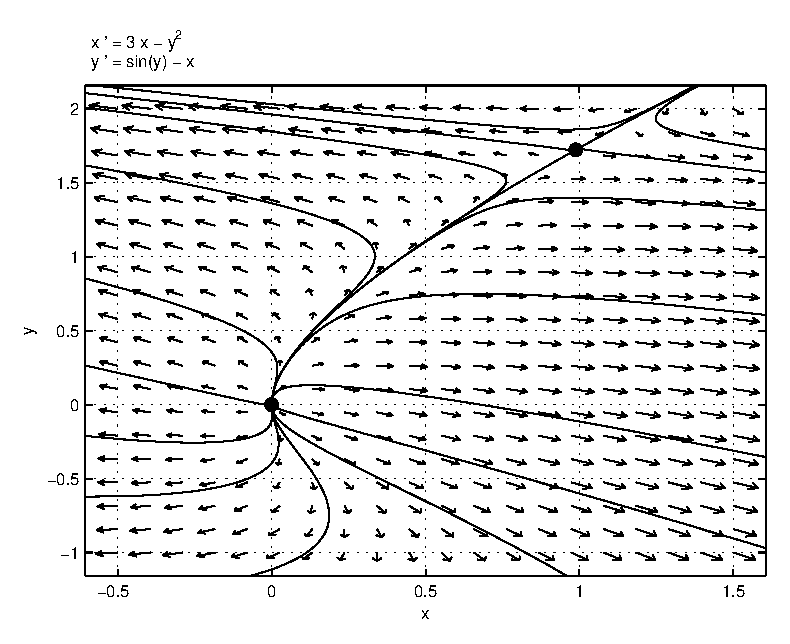
\includegraphics[width=5in]{pplane_plots/NonlinExample1.ps}
}
\caption{Phase portrait for system \eqref{eqn:nonlinexample1}.}
\label{fig:nonlinexample1}
\end{figure}
  The Jacobian matrix is
\begin{equation}
  J = \begin{bmatrix}
           3 &  -2y \\
	   -1 & \cos(y)
      \end{bmatrix}
\end{equation}
and at $(0,0)$, this is
\begin{equation}
  J = \begin{bmatrix}
           3 &  0 \\
	   -1 & 1
      \end{bmatrix}.
\end{equation}
The eigenvalues are $\lambda_1=1$ and $\lambda_2=3$.
Both $\lambda_1>0$ and $\lambda_2>0$, so the origin
in the linearization is a \emph{source}.
Since the real part of both eigenvalues is nonzero,
we conclude that the equilibrium $(0,0)$ of the original
nonlinear equations is also a source.
\emph{Near $(0,0)$}, the linearization provides a
good approximation to the nonlinear system.
The image on the left in Figure~\ref{fig:nonlinexample1compare}
shows the phase portrait of \eqref{eqn:nonlinexample1}
near $(0,0)$, and the image on the right
is the phase portrait of the linearization at $(0,0)$.
\begin{figure}
\centerline{%
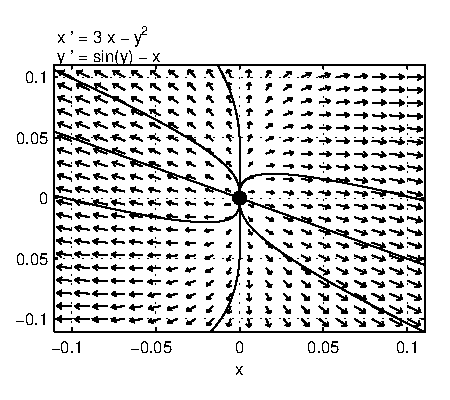
\includegraphics[width=2.5in]{pplane_plots/NonlinExample1detail.ps}
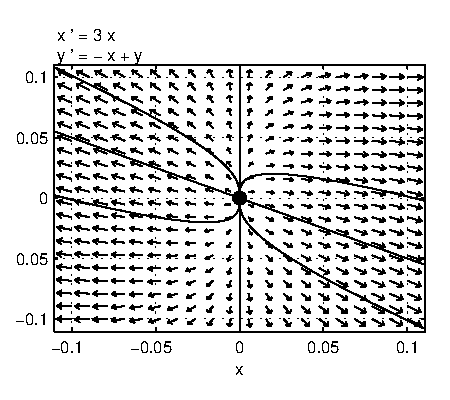
\includegraphics[width=2.5in]{pplane_plots/NonlinExample1lin.ps}
}
\caption{On the left is the phase portrait of
\eqref{eqn:nonlinexample1} near $(0,0)$, and on the
right is the phase portrait of the linearization
at $(0,0)$.  They are almost the same.  If we zoomed
in closer, they would appear even more similar.}
\label{fig:nonlinexample1compare}
\end{figure}
\end{xexample}
%
%
\begin{xexample}
The system of differential equations
\begin{equation}
\begin{split}
  \frac{dx}{dt} & = 2x - y -x^2 \\
  \frac{dy}{dt} & = x - 2y + y^2
\end{split}
\end{equation}
has equilibria at $(0,0)$ and $(1,1)$.
The Jacobian matrix is
\begin{equation}
  J = \begin{bmatrix}
           2-2x & -1 \\
	   1 & -2 + 2y
      \end{bmatrix}
\end{equation}

At $(0,0)$, this is
\begin{equation}
  J = \begin{bmatrix}
           2 & -1 \\
	   1 & -2
      \end{bmatrix}
\end{equation}
This matrix has eigenvalues $\lambda_1 = -\sqrt{3}$ 
and $\lambda_2 = \sqrt{3}$, so the
origin of the  linearized system is a saddle point.
Both eigenvalues are real and nonzero,
so we conclude that the equilibrium
$(0,0)$ of the nonlinear system is also a saddle point.

At $(1,1)$, the Jacobian matrix is
\begin{equation}
  J = \begin{bmatrix}
           0 & -1 \\
	   1 & 0
      \end{bmatrix}
\end{equation}
This matrix has eigenvalues $\lambda=\pm i$,
so the linearization results in a \emph{center}.
Because the real parts of the eigenvalues are
zero, we can \emph{not} conclude that $(1,1)$
is actually a center in the nonlinear system.
Trajectories near $(1,1)$ will rotate around $(1,1)$, but
the linearization can not tell us if these trajectories
actually form closed curves.
The trajectories might, in fact, slowly spiral
towards or away from $(1,1)$.
\end{xexample}
%
\newpage
%
% \begin{exercises}
% \begin{exercise}
% An exercise...
% \end{exercise}
% \end{exercises}
%
\section{Periodic Solutions}
It is possible that solutions can oscillate...
% \begin{exercises}
% \begin{exercise}
% An exercise...
% \end{exercise}
% \begin{exercise}
% Another exercise...
% \end{exercise}
% \end{exercises}
% 
% \newpage

\section{Higher Dimensional Systems}
\[
  \dot{\BX} = \BF(\BX)
\]
\begin{xexample}
\emph{Do a 3D example: solve for equilibria, find the
Jacobian, determine stability.  At least one point
should require numerical evaluation of the equilibrium
and of the eigenvalues of the Jacobian.}
\end{xexample}
%

\section{The Saddle-Node Bifurcation}
\index{saddle-node bifurcation}

\section{The Hopf Bifurcation}
\index{Hopf bifurcation}

\section{Chaos}
Just an example...

\begin{exercises}
\begin{exercise}
An exercise... use a computer to observe chaotic solutions
to the Lorenz equations.
\end{exercise}
\begin{exercise}
Another exercise...
\end{exercise}
\end{exercises}
%
%
%%%%%%%%%%%%%%%%%%%%%%%%%%%%%%%%%%%%%%%%%%%%%%%%%%%%%%%%%%%
%

\chapter{Applications of Differential Equations}
%
In this chapter, we developed models using differential
equations for a wide variety of systems.
We include problems from a wide variety of fields:
\begin{itemize}
\item \emph{Economics}: Solow growth model
\item \emph{Population Dynamics}: predator-prey, competing species
\item \emph{War and Peace}: Lanchester battle model, Richardson's arms
race model
\item \emph{Love Affairs}: a variation of Romeo and Juliet, Rinaldi's
model of Petrarch's love for Laura
\item \emph{Epidemiology}: the SI, SIR, and SIQR models
\end{itemize}
%
\newpage
%
\section{Solow's Economic Growth Model}
\index{Solow growth model}
% \emph{(Draft version\footnote{\copyright ~2006 Warren Weckesser}.)}

%\medskip
We consider a model from macroeconomics.\index{economics}
Let $K$ be the capital,%
\footnote{\emph{Capital} includes things that are owned to be used
in production, such as buildings and manufacturing equipment.}%
~$L$ the labor, and $Q$ the production output of an economy.
We are interested in a \emph{dynamic} problem, so $K(t)$, $L(t)$ and
$Q(t)$ are all functions of time, but we will suppress the $t$ argument.
In elementary economics, one learns that a common assumption is that
$Q$ can be expressed as function of $K$ and $L$:
\begin{equation}
   Q = f(K,L).
   \label{EQN:PROD}
\end{equation}
%We make the reasonable assumptions that $f_K > 0$ and $f_L > 0$.
%(The subscript denotes a partial derivative: $f_K = \partial f/\partial K$.)
%These assumptions mean that $Q$ increases if either $K$ or $L$ increases.
%That is, with more capital or more labor, we can produce more.
%We also assume that $f_{KK} < 0$ and $f_{LL} < 0$.
%These assumptions say that $f$ has \emph{diminishing returns} to the
%inputs $K$ and $L$.  In other words, the larger $K$ is, the less is the
%effect of increasing $K$, and the same holds for $L$.
We assume that $f$ has, using economics terminology,
\emph{constant returns to scale}.\index{constant returns to scale}  Mathematically, this means
that multiplying $K$ and $L$ by the same amount results in $Q$ being
multiplied by the same amount.  That is, for any constant $b$,
\begin{equation}
   f(bK,bL) = bf(K,L).
\end{equation}
For example, the Cobb-Douglas function\index{Cobb-Douglas function}
$f(K,L) = K^{1/3}L^{2/3}$
satisfies this assumption.

We make two more assumptions.
We assume that a constant proportion of $Q$ is invested in capital.
This means that the \emph{rate of change} of $K$ is proportional to
$Q$:
\begin{equation}
    \frac{dK}{dt} = s Q,
\label{EQN:DKDT}
\end{equation}
where $s > 0$ is the proportionality constant.
We also assume that the labor force is growing according
to the equation
\begin{equation}
   \frac{dL}{dt} = \lambda L,
   \label{EQN:DLDT}
\end{equation}
where $\lambda > 0$ is the per capita growth rate.  This is a
familiar first order equation for $L$ which we can solve to find 
\begin{equation}
    L = L_0 e^{\lambda t}.
\label{eqn:solowLsol}
\end{equation}

If possible, we would like to combine \eqref{EQN:PROD},
\eqref{EQN:DKDT}, and \eqref{EQN:DLDT} (or \eqref{eqn:solowLsol})
into a single
equation that we may easily analyze. A natural first
attempt is to substitute \eqref{EQN:PROD} into
\eqref{EQN:DKDT} and use \eqref{eqn:solowLsol} to obtain
\begin{equation}
  \frac{dK}{dt} = sf(K,L_0e^{\lambda t})
\label{eqn:solowfirstattempt}
\end{equation}
This is a first order differential equation for $K(t)$.
It is, however, nonautonomous; the right side depends on $t$ explicitly.
We could try to analyze this equation, but it would
be nice if we could find an \emph{autonomous} first order
differential equation.  It turns out we can derive an
autonomous equation for 
the \emph{ratio} $\frac{K}{L}$ instead of $K$.

First, because $f$ has constant returns to scale,
we may write
\begin{equation}
  f(K,L) = f\left(L\frac{K}{L},L\right) = Lf\left(\frac{K}{L},1\right).
\end{equation}
Then, after dividing by $L$, \eqref{eqn:solowfirstattempt} becomes
\begin{equation}
  \frac{1}{L}\frac{dK}{dt} = sf\left(\frac{K}{L},1\right)
\label{eqn:solowintermediate}
\end{equation}
Next, we consider the
derivative of $\frac{K}{L}$ given by the quotient rule,
and we use \eqref{EQN:DLDT}:
\begin{equation}
  \frac{d}{dt}\left(\frac{K}{L}\right)
    = \frac{1}{L}\frac{dK}{dt} - \frac{K}{L^2}\frac{dL}{dt}
    = \frac{1}{L}\frac{dK}{dt} - \lambda\frac{K}{L}.
\end{equation}
If we subtract $\lambda\frac{K}{L}$ from both sides of
\eqref{eqn:solowintermediate}, the left side becomes
$\frac{d}{dt}\left(\frac{K}{L}\right)$, and we obtain
\begin{equation}
  \frac{d}{dt}\left(\frac{K}{L}\right) =
    sf\left(\frac{K}{L},1\right) - \lambda\frac{K}{L}
\label{eqn:solowKoverL}
\end{equation}
We now have an equation in which the unknown function
is $\frac{K}{L}$.  Let us define
\begin{equation}
   k = \frac{K}{L}
\label{eqn:solowdefk}
\end{equation}
and
\begin{equation}
    g(k) = f(k,1).
\label{eqn:solowdefg}
\end{equation}
Then \eqref{eqn:solowKoverL} becomes
\begin{equation}
  \frac{dk}{dt} = s g(k) - \lambda k
\end{equation}
This is the \emph{Solow Growth Model} \cite{Solow}\index{Solow growth model}
which models the growth of the ratio of capital to labor
under the assumptions given earlier.

\medskip
\fbox{%
\begin{minipage}{4.7in}
\medskip
\centerline{\textbf{Summary}}
\medskip
\emph{Assumptions}
\\[3pt]
\hspace*{0.15cm}(1) $Q=f(K,L)$ where $f(K,L)$ is a function
with constant returns to scale.
\\[4pt]
\hspace*{0.15cm}(2) $\ds \frac{dK}{dt} = sQ$; a fraction of the production output
is invested in capital.
\\[4pt]
\hspace*{0.15cm}(3) $\ds \frac{dL}{dt} = \lambda L$; labor grows according to this
equation.
\\[6pt]
\emph{Definitions}
\\[3pt]
\hspace*{0.25cm}$\bullet$ $\ds k = \frac{K}{L}$; we analyze the \emph{ratio} of capital to labor.
\\[3pt]
\hspace*{0.25cm}$\bullet$ $g(k) = f(k,1)$.
\\[6pt]
\emph{Result}\\
\centerline{$\ds \frac{dk}{dt} = s g(k) - \lambda k$}
\medskip
\end{minipage}
}

\medskip
\begin{xexample}
\label{exm:solow}
As an example, let's take the production function to be
\begin{equation}
   f(K,L) = K^{1/3}L^{2/3}.
\label{eqn:cobbexample}
\end{equation}
Then
\begin{equation}
g(k) = f(k,1) = k^{1/3},
\end{equation}
 and the differential equation for
$k$ is
\begin{equation}
   \frac{dk}{dt} = sk^{1/3} - \lambda k .
\label{eqn:solowcobb}
\end{equation}
Figure~\ref{fig:solow_rhsplot} shows the graph of
$\frac{dk}{dt}$ versus $k$.
\begin{figure}
\centerline{\includegraphics[width=2.75in]{matlab/solow_rhsplot.eps}}
\caption{The graph of the right side of equation \eqref{eqn:solowcobb}.}
\label{fig:solow_rhsplot}
\end{figure}

By solving
\[
   sk^{1/3} - \lambda k = 0,
\]
we find the equilibrium solutions to be $k=0$ or $k=(s/\lambda)^{3/2}$.


Changing $\lambda$ or $s$ will change the scale
(and the numerical value of the non-zero equilibrium),
but the graph of $dk/dt$ versus $k$ will always have the
same qualitative shape as the graph shown above.

We see that if $k>0$ is small,
$\frac{dk}{dt} > 0$, so $k$
will increase; the equilibrium $k=0$ is \emph{unstable}.
The graph of $k(t)$ will have an inflection point when $k$ reaches
$\left(\frac{s}{3\lambda}\right)^{3/2}$
(where right side of \eqref{eqn:solowcobb} has its maximum).
$k$ will then converge asymptotically to the non-zero equilibrium.

The equilibrium $k=(s/\lambda)^{3/2}$ is \emph{asymptotically stable}:
any solution that starts near the equilibrium will converge to the equilibrium
as $t\rightarrow \infty$.
In fact, \emph{all} solutions with $k(0)>0$ will converge asymptotically to this
equilibrium.

What does this mean in terms of the capital $K$ and the labor $L$?
Since $k(t) = K(t)/L(t)$, and $L(t) = L_0e^{\lambda t}$, if $k(t)$ converges to an
asymptotically stable equilibrium $k_1$, then $K(t)$ must behave asymptotically like
$k_1  L(t)$.  This means that, in the long term, $K(t)$ must 
grow exponentially, with the
same exponent as $L(t)$.
This model predicts that in the long term, capital will grow
exponentially along with the labor.
If, for example, the capital is too low, it will rapidly increase until it becomes
approximately proportional to the labor, and then it will settle into a long term behavior in
which capital remains proportional to the labor.
\end{xexample}
%
\begin{exercises}
\begin{exercise}
Verify that the maximum value of the right side
of \eqref{eqn:solowcobb} occurs
at $k=\left(\frac{s}{3\lambda}\right)^{3/2}$.
\end{exercise}
\begin{exercise}
Find an explicit solution for \eqref{eqn:solowcobb},
assuming that the initial condition is $k(0)=k_0 > 0$.
Use your solution to verify analytically that
$\lim_{t\rightarrow\infty} k(t) = \left(s/\lambda\right)^{3/2}$.
\end{exercise}
\begin{exercise}
Suppose that labor grows according to a logistic equation
\begin{equation}
  \frac{dL}{dt} = \lambda L \left(1-\frac{L}{M}\right)
\end{equation}
where $M$ is the carrying capacity for the labor population.
Derive a new differential equation for $k(t)$.
Is your new equation autonomous?
If not, can you still determine the asymptotic
behavior of the solutions as $t\rightarrow\infty$?
\end{exercise}
\begin{exercise}
Suppose we include the fact that capital deteriorates
over time.  We replace the assumption given
in equation \eqref{EQN:DKDT} with
\begin{equation}
   \frac{dK}{dt} = -rK + sQ
\end{equation}
where $r > 0$.
(This says that, if $Q=0$, then $K$ will decay and
approach zero asymptotically.)
\begin{enumerate}
\item[(a)]
Show that this leads to the differential equation
\begin{equation}
   \frac{dk}{dt} = s g(k) - (r+\lambda) k,
\end{equation}
where $k$ and $g(k)$ are defined
in \eqref{eqn:solowdefk} and \eqref{eqn:solowdefg}, 
respectively.
\item[(b)]
Suppose the production function is the Cobb-Douglas function
given in equation \eqref{eqn:cobbexample}.
Find the equilibrium solutions of this model, 
and describe the behavior of all possible solutions
(assuming $k(0)>0$).
Compare to the results given in Example \ref{exm:solow}.
\end{enumerate}
\end{exercise}
\begin{exercise}
Find an explicit solution to equation
\eqref{eqn:solowfirstattempt} when $f$ is given by
\eqref{eqn:cobbexample}.  (The equation will be separable.)
Then divide your solution by $L$ to obtain $k(t)$,
and verify that $\lim_{t\rightarrow\infty} k(t) =
\left(s/\lambda\right)^{3/2}$.
\end{exercise}
\begin{exercise}
Consider a general Cobb-Douglas function with
constant returns to scale
\begin{equation}
   f(K,L) = K^{\alpha}L^{1-\alpha}
\end{equation}
where $0 < \alpha < 1$.
Repeat the analysis of Example \ref{exm:solow},
but use this function in place of the
specific function given in \eqref{eqn:cobbexample}.
\end{exercise}
\end{exercises}
\newpage
%
\section{Predator-Prey\index{predator-prey}}
%
\newpage
%
\section{Competing Species\index{competing species}}
%
We consider an example that models the populations
of two species that are competing for a common resource.
In the absence of the other species, each species
grows according to a logistic equation.
However, the presence of one species lowers
the \emph{per capita} growth rate of the other species.
One way to write the equations for this system
is
\begin{equation}
\begin{split}
  \frac{dx}{dt} & = r_1\left(1-\frac{x}{K_1}-\beta_1 y\right)x \\
  \frac{dy}{dt} & = r_2\left(1-\frac{y}{K_2}-\beta_2 x\right)y
\end{split}
\end{equation}
Note that if $y(0)=0$, then $y(t)$ remains $0$, and
the equation for $x(t)$ is
\begin{equation}
    \frac{dx}{dt} = r_1 \left(1-\frac{x}{K_1}\right),
\end{equation}
which is the familiar logistic equation.
Similarly, if $x(0)=0$, then $x(t)$ remains $0$ and
$y(t)$ is governed by a logistic equation.

Let's do a careful analysis of a specific example,
in which $r_1 = 1$, $K_1 = 1$, $\beta_1 = 1$, 
$r_2 = 3/4$, $K_2 = 3/4$, and $\beta_2 = 2/3$.
The differential equations are
\begin{equation}
\begin{split}
  \frac{dx}{dt} & = (1-x-y)x \\
  \frac{dy}{dt} & = \frac{3}{4}\left(1 -\frac{4}{3}y - \frac{2}{3}x\right)y .
\end{split}
\label{eqn:compspecexample}
\end{equation}
We'll find the equilibria, find the linearization at each
equilibrium to determine the behavior near each one, and then
use the nullclines of~\eqref{eqn:compspecexample} to understand
what happens in the phase plane ``far away'' from the equilibria.

\noindent
\textbf{Equilibria.}
To find the equilibria, we must solve
\begin{equation}
\begin{split}
(1-x-y)x & = 0 \\
\frac{3}{4}\left(1 -\frac{4}{3}y - \frac{2}{3}x\right)y & = 0.
\end{split}
\label{eqn:exampleequil}
\end{equation}
The first equation holds if $x=0$ or $y = 1-x$.
We consider each case separately in the second equation.
\begin{itemize}
\item
If $x=0$, then the second equation of~\eqref{eqn:exampleequil} implies
$y=0$ or $y=\frac{3}{4}$.

So two equilibria are $(0,0)$ and $(0,3/4)$.
\item
If $y=1-x$, then the second equation
of~\eqref{eqn:exampleequil} implies
\begin{equation}
  \left(1-\frac{4}{3}(1-x) - \frac{2}{3}x\right)(1-x) = 0
  \implies x=1 \quad \textrm{or} \quad x=\frac{1}{2}.
\end{equation}
So two equilibria are $(1,0)$ and $(1/2,1/2)$.
\end{itemize}

\noindent
\textbf{Linearization at each equilibrium.}
We have found the following equilibria: $(0,0)$, $(0,3/4)$, $(1,0)$, $(1/2,1/2)$.
We now determine the behavior of~\eqref{eqn:compspecexample}
near each equilibrium by finding the linearization at each
equilibrium.
We will need the Jacobian matrix:
\begin{equation}
  J = \begin{bmatrix}
          1-2x-y & -x \\
	  -\frac{1}{2}y & \frac{3}{4}-2y-\frac{1}{2}x
      \end{bmatrix}
\end{equation}
For each equilibrium, we will find the Jacobian matrix
and plot the phase portrait of the linearization.
We make two remarks about the phase portraits of the linearized
systems:
\begin{enumerate}
\item
Recall from the notes on ``Linearization'' that we
used the local coordinates $(u,v)$ for the linearization.
In a linear system, the scale of the coordinates is not
important: if you zoom in on the origin of a linear system,
the phase portrait will look exactly the same.
So, in the following phase portraits of the linearizations,
the ranges on the axis are  from $-1$ to $1$.  These
are \emph{not} the actual $x$ and $y$ ranges.
\item
In a population model such as this, $x<0$ and $y<0$
are not relevant.  However, we will still plot negative
values in the linearization.  It seems easier to simply
plot the linear phase portrait, ignoring the actual
meaning until later.  Also, recall that the linearized
system is expressed in coordinates measured relative
to the equilibrium.  If a coordinate of the equilibrium
is positive, then a negative value of the corresponding
local coordinates means that the population is less than
the equilibrium value. It does not necessarily mean that
the actual population is negative.
\end{enumerate}

\medskip

At $(0,0)$, the Jacobian matrix is
\begin{equation}
  J = \begin{bmatrix}
          1 & 0 \\
	  0 & \frac{3}{4} \\
      \end{bmatrix} .
\end{equation}
The eigenvalues are $\lambda_1 = 3/4$ and $\lambda_2 = 1$, with
corresponding eigenvectors
\[
  \BV_1 = \begin{bmatrix} 0 \\ 1 \end{bmatrix}
  \quad \textrm{and}\quad 
  \BV_2 = \begin{bmatrix} 1 \\ 0 \end{bmatrix}.
\]
Since $\lambda_1 > 0$ and $\lambda_2 > 0$,
the equilibrium $(0,0)$ is a
\emph{source}.  The trajectories come out of $(0,0)$
tangent to the eigenvector $\BV_1$.
The phase portrait of the linearization at $(0,0)$ is
shown in Figure~\ref{fig:CompSpecLinPlots}(a).
%\centerline{%
%\includegraphics{matlab/LinCS1.eps}
%}
%\noindent
If we were to ``zoom in'' on the point $(0,0)$
in~\eqref{eqn:compspecexample}, this is what the 
phase portrait would look like.

%\medskip

At $(1,0)$, the Jacobian matrix is
\begin{equation}
  J = \begin{bmatrix}
          -1 & -1 \\
	  0 & \frac{1}{2} \\
      \end{bmatrix}.
\end{equation}
The eigenvalues are $\lambda_1 = -1$ and $\lambda_2 = 1/2$,
with corresponding eigenvectors
\[
  \BV_1 = \begin{bmatrix} 1 \\ 0 \end{bmatrix}
  \quad \textrm{and} \quad
  \BV_2 = \begin{bmatrix} 1 \\ -3/2 \end{bmatrix}.
\]
Since $\lambda_1 < 0$ and $\lambda_2 > 0$, the equilibrium
$(1,0)$ is a \emph{saddle point}.
The phase portrait of the linearization at $(1,0)$ is
shown in Figure~\ref{fig:CompSpecLinPlots}(b).

%\centerline{%
%\includegraphics{matlab/LinCS2.eps}
%}

%\medskip

At $(0,3/4)$, the Jacobian matrix is
\begin{equation}
  J = \begin{bmatrix}
          \frac{1}{4} & 0 \\
	  -\frac{3}{8} & -\frac{3}{4} \\
      \end{bmatrix}.
\end{equation}
The eigenvalues are $\lambda_1 = -\frac{3}{4}$ and
$\lambda_2 = \frac{1}{4}$,
with corresponding eigenvectors
\[
  \BV_1 = \begin{bmatrix} 1 \\ -3/8 \end{bmatrix}
  \quad \textrm{and}\quad 
  \BV_2 = \begin{bmatrix} 0 \\ 1 \end{bmatrix}.
\]
Since $\lambda_1 < 0$ and $\lambda_2 > 0$,
the equilibrium $(0,3/4)$
is a \emph{saddle point}.
The phase portrait of the linearization at $(0,3/4)$ is
shown in Figure~\ref{fig:CompSpecLinPlots}(c).

%\centerline{%
%\includegraphics{matlab/LinCS3.eps}
%}

%\medskip

At $(1/2,1/2)$, the Jacobian matrix is
\begin{equation}
  J = \begin{bmatrix}
          -\frac{1}{2} & -\frac{1}{2} \\
	  -\frac{1}{4} & -\frac{1}{2} \\
      \end{bmatrix}.
\end{equation}
The eigenvalues are
$\lambda_1 = \frac{-2-\sqrt{2}}{4} \approx -0.853 < 0$
and $\lambda_2 = \frac{-2+\sqrt{2}}{4} \approx -0.147 < 0$,
with corresponding eigenvectors
\[
  \BV_1 = \begin{bmatrix} \sqrt{2} \\ 1 \end{bmatrix}
  \quad \textrm{and}\quad
  \BV_2 = \begin{bmatrix} \sqrt{2} \\ -1 \end{bmatrix}.
\]
Since both eigenvalues are negative,
the equilibrium at $(1/2,1/2)$ is a \emph{sink}.
The phase portrait of the linearization at $(1/2,1/2)$ is
shown in Figure~\ref{fig:CompSpecLinPlots}(d)

%\centerline{%
%\includegraphics{matlab/LinCS4.eps}
%}

%\medskip

\begin{figure}
\centerline{\includegraphics[width=2.5in]{matlab/LinCS1.eps}\includegraphics[width=2.5in]{matlab/LinCS2.eps}}
\vspace{-0.2in}
\centerline{\hspace{0.2in}\textbf{(a)}\hspace{2.1in}\textbf{(b)}}
\centerline{\includegraphics[width=2.5in]{matlab/LinCS3.eps}\includegraphics[width=2.5in]{matlab/LinCS4.eps}}
\vspace{-0.2in}
\centerline{\hspace{0.2in}\textbf{(c)}\hspace{2.1in}\textbf{(d)}}
\caption{Phase portraits of the linearizations at each equilibrium point
of the competing species example:
(a) at $(0,0)$; (b) at $(1,0)$; (c) at $(0,3/4)$; (d) at $(1/2,1/2)$.}
\label{fig:CompSpecLinPlots}
\end{figure}


\noindent
\textbf{Nullclines.}
Since the eigenvalues at each linearization
all had nonzero real parts, each linearization
provides a good approximation to the behavior
of~\eqref{eqn:compspecexample} near the corresponding
equilibrium point.
However, the local linearizations do not tell us what is
happening in the phase plane far from the equilibria.
In a planar system such as this, the nullclines
can provide useful information about the phase portrait.

The $x$ nullcline is given by
\begin{equation}
   (1-x-y)x = 0 \implies x=0 \quad\textrm{or}\quad y = 1-x.
\end{equation}
So $\frac{dx}{dt}=0$ on the lines\footnote{In this example, and in all
the planar linear systems that we have studied,
the nullclines are straight lines. This is not true in general;
nullclines can be curves.}
$x=0$ and $y=1-x$.

The $y$ nullcline is given by
\begin{equation}
  \frac{3}{4}\left(1-\frac{4}{3}y - \frac{2}{3} x\right)y = 0
\end{equation}
which gives the lines
\begin{equation}
  y = 0 \quad \textrm{or} \quad y = \frac{3}{4} - \frac{1}{2}x.
\end{equation}
On these lines, $\frac{dy}{dt}=0$.

The nullclines give the points in the plane where 
$\frac{dx}{dt}=0$ or $\frac{dy}{dt}=0$.
They form the boundaries of regions in the plane
where $\frac{dx}{dt}$ and $\frac{dy}{dt}$ do not change sign.
This can be very useful information.
For example, if we know that in a certain region,
$\frac{dx}{dt} > 0$ and $\frac{dy}{dt}>0$, we know that all
vectors of the vector field point ``up and to the right'';
this means all trajectories move up and to the right.
If this region is in the first quadrant, it implies that
all trajectories move away from the origin.

In the following plot, the nullclines (that are not coordinate
axes) are plotted with dashed lines, and trajectories
are plotted as solid lines.  Since our equations give 
a model for two species, we only include the first quadrant.
Negatives values would not be meaningful, so we do not include them.

\smallskip
\centerline{%
\fbox{\includegraphics[width=4.5in]{matlab/CompSpec.eps}}
}

\medskip
\noindent
In the region labeled \textsf{\textbf{A}},
$\frac{dx}{dt}<0$ and $\frac{dy}{dt}<0$.
All trajectories in this region (which extends out to infinity)
must move down and to the left.  This implies that
all these trajectories must either cross the $x$ or $y$ axes,
or cross the nullclines that form the boundaries between
\textsf{\textbf{A}} and \textsf{\textbf{B}}
and between \textsf{\textbf{A}} and \textsf{\textbf{D}}.
But the coordinate axes are themselves solutions,
so solutions that do not start on the coordinate axes
can not cross the axes.  Thus any trajectory that begins in
\textsf{\textbf{A}} must eventually cross into
\textsf{\textbf{B}} or \textsf{\textbf{D}}
(or, in one special case, converge to the equilibrium
at $(1/2,1/2)$).

Now consider trajectories in \textsf{\textbf{B}}.
In \textsf{\textbf{B}}, we have
$\frac{dx}{dt} > 0$ and $\frac{dy}{dt} < 0$.
All trajectories in this region move down and to the right.
They can not cross either of the nullclines that
form the upper and lower boundaries of the region,
because the vector field on these nullclines points
\emph{into} \textsf{\textbf{B}}.  Therefore,
\emph{all trajectories in \textsf{\textbf{B}} must
converge to $(1/2,1/2)$}.

A similar argument applies to \textsf{\textbf{D}},
where $\frac{dx}{dt} < 0$ and $\frac{dy}{dt} >0$.
In this region, all trajectories move up and to the left,
but they can't cross the nullclines, so
\emph{all trajectories in \textsf{\textbf{D}} must
converge to $(1/2,1/2)$}.

Finally, in \textsf{\textbf{C}} we have
$\frac{dx}{dt} >0$ and $\frac{dy}{dt} > 0$.
All trajectories in this region move up and to the right.
Therefore, they must all eventually cross into
\textsf{\textbf{B}} or \textsf{\textbf{D}}, except
for the special trajectory in \textsf{\textbf{C}}
that converges to $(1/2,1/2)$.

Our conclusion is that any trajectory that begins in the
first quadrant, with $x(0)>0$ and $y(0)>0$, must
converge to $(1/2,1/2)$. Note that we have concluded this
without actually solving the differential equations
given in~\eqref{eqn:compspecexample}.
Thus, this population model
predicts that the two species will co-exist in 
a stable equilibrium.
(Different parameters values may lead to different
conclusions.)

% \begin{exercises}
% \begin{exercise}
% An exercise...
% \end{exercise}
% \end{exercises}
%
\newpage
%
\section{Battle of Attrition--The Lanchester Model}
\index{Lanchester model}
%
We consider a model of a battle in which the opponents
simply blast away at each other until one side is wiped
out.
This model was proposed by F. W. Lanchester\cite{Lanchester}.
The simple version presented here
is \emph{not} a realistic model of modern warfare!
%(It has been suggested as a model for the battles that
%occur between colonies of ants...\emph{find this reference!})
In this model $x(t)$ and $y(t)$ are the sizes of the
opposing armies at time $t$.
As the battle rages, the losses incurred by army $x$
are simply proportional to the size of army $y$,
and the losses incurred by army $y$ are proportional
to the size of army $x$ (but not necessarily with
the same proportionality constant).
That is,
\begin{equation}
\begin{split}
   \frac{dx}{dt} & = - \alpha y \\
   \frac{dy}{dt} & = - \beta x
\end{split}
\end{equation}
where $\alpha$ and $\beta$ are positive constants.
This is a planar linear system.
The coefficient matrix is
\begin{equation}
  A = \begin{bmatrix} 0 & -\alpha \\ -\beta & 0 \end{bmatrix}.
\end{equation}
The eigenvalues are $\lambda_1 = -\sqrt{\alpha\beta}$
and $\lambda_2 = \sqrt{\alpha\beta}$,
so we know that the origin $(0,0)$ is a saddle point.
A corresponding set of eigenvectors are
\[
  \BV_1 = \begin{bmatrix} 1 \\ -\sqrt{\frac{\beta}{\alpha}}\end{bmatrix}
  \quad \textrm{and}\quad
  \BV_2 = \begin{bmatrix} 1 \\ \sqrt{\frac{\beta}{\alpha}}\end{bmatrix}.
\]
The $x$ nullcline is $y=0$, which means that trajectories
cross the $x$ axis vertically. Similarly, the $y$ nullcline is
$x=0$, so trajectories cross the $y$ axis horizontally.
Since the nullclines are the axes, we know that in the first
quadrant, $dx/dt < 0$ and $dy/dt < 0$, so for any initial
condition in the first quadrant, the trajectory will eventually
cross either the $x$ or $y$ axis. If the initial condition
happens to be in the eigenspace associated with the negative
eigenvalue $\lambda_1$, the trajectory will converge to
$(0,0)$. (In this exceptional case, the armies wipe each
other out!)
This eigenspace is given by the line
\begin{equation}
  y = \sqrt{\frac{\beta}{\alpha}}\, x.
\label{eqn:lanchester_eigenspace}
\end{equation}
If the initial condition is above the $\lambda_1$ eigenspace
(so $y_0 > \sqrt{\frac{\beta}{\alpha}}\, x_0$), then
$y$ wins, and if the initial condition is below this line,
then $x$ wins.

There is a different approach we can take to analyze
this system.
By multiplying the first equation by $2\beta x$ and the
second by $-2\alpha y$, we obtain
\begin{equation}
\begin{split}
 2\beta x\frac{dx}{dt} & = -2 \alpha \beta x y \\
 -2\alpha y\frac{dy}{dt} & = 2 \alpha \beta x y.
\end{split}
\end{equation}
Then adding these equations results in
\begin{equation}
   2\beta x\frac{dx}{dt} -2\alpha y\frac{dy}{dt} = 0.
\end{equation}
We note that the left side of this equation is
the $t$ derivative of $\beta x^2 - \alpha y^2$.
So we'll integrate from $0$ to $t$:
\begin{equation}
   \int_0^t \left(2\beta x\frac{dx}{dt} -2\alpha y\frac{dy}{dt}\right)\, ds = \int_0^t 0 \, ds = 0.
\end{equation}
which gives
\begin{equation}
\begin{split}
  \left.\beta x^2(s) - \alpha y^2(s)\right|_{s=0}^{s=t} & = 0 \\
   \beta x^2(t) - \alpha y^2(t) - (\beta x^2(0) - \alpha y^2(0)) & = 0 \\
      \beta x^2(t) - \alpha y^2(t) & = \beta x^2(0) - \alpha y^2(0) =
         \beta x_0^2 - \alpha y_0^2 \\
\end{split}
\end{equation}
By dropping the explicit $t$ dependence of $x(t)$
and $y(t)$, we obtain
\begin{equation}
   \beta x^2 - \alpha y^2 = \beta x_0^2 - \alpha y_0^2.
   \label{eqn:lanchester_hyperbola}
\end{equation}
This is the equation of a hyperbola in the $(x,y)$ plane.
Whether the hyperbola crosses the $x$ or $y$ axis is
determined by the sign of
$\beta x_0^2 - \alpha y_0^2$.
If this value is positive, then the hyperbola
crosses the positive $x$ axis
at $x=\sqrt{x_0^2 - \frac{\alpha}{\beta} y_0^2}$.
If $\beta x_0^2 - \alpha y_0^2$
is negative, then the hyperbola
crosses the $y$ axis at
$y = \sqrt{y_0^2 - \frac{\beta}{\alpha} x_0^2}$.
Thus, if we know the initial sizes of the armies
and the constants $\alpha$ and $\beta$, we can
easily determine which army will win, and what the
size of the winning army will be at the end of the
battle.

\begin{xexample}
\label{exm:Lanchester}
Suppose we have two armies, with $\alpha=1.0$,
$\beta = 1.5$, and $x_0=10,000$.
What is the outcome of the battle if
$y_0=10,000$?  What if $y_0=14,000$?
How large must $y_0$ be if both armies
wipe each other out?

We can answer these questions with
equation \eqref{eqn:lanchester_hyperbola}.
We have
\begin{equation}
  1.5x^2-y^2 = 1.5(10000)^2-y_0^2
\end{equation}
If $y_0=10,000$, we have
\begin{equation}
  1.5x^2-y^2 = 1.5(10000)^2-(10000)^2 = 5\times 10^7.
\end{equation}
The right side is positive, so the hyperbola must cross
the $x$ axis.  That is, the $x$ army wins, and the
size of the surviving army is
\begin{equation}
   x = \sqrt{\frac{5\times 10^7}{1.5}} \approx 5800.
\end{equation}
If $y_0=14,000$, we have
\begin{equation}
  1.5x^2-y^2 = 1.5(10000)^2-(14000)^2 = -4.6\times 10^7.
\end{equation}
The right side is negative, so the hyperbola must
cross the $y$ axis.  The $y$ army wins, and its remaining size
is
\begin{equation}
   y = \sqrt{4.6\times 10^7} \approx 6780.
\end{equation}
The armies will wipe each other out when
\begin{equation}
  y_0 = \sqrt{\frac{\beta}{\alpha}}x_0 
      = \sqrt{\frac{1.5}{1.0}}10000
      \approx 12247.
\end{equation}
Plots of the three curves in the $xy$ plane for each of these
cases are shown in Figure~\ref{fig:LanchesterExamplePlots}.
\begin{figure}
\centerline{\includegraphics[width=2in]{matlab/LanchesterExamplePlots.eps}}
\caption{Plots of the three curves discussed in
Example~\ref{exm:Lanchester}.}
\label{fig:LanchesterExamplePlots}
\end{figure}
\end{xexample}

Equation \eqref{eqn:lanchester_eigenspace} gives an asymptote
of the family of hyperbolas.
If the initial sizes of the armies result in a point
on this line, the two armies will eliminate each other.
The equation lets us make an interesting observation.
Suppose $x_0$ is, say, three times larger than $y_0$.
How much more efficient must the $y$ army be in order to
defeat the larger opponent?
In other words, by what factor must $\alpha$
exceed $\beta$
to ensure that $y_0 > \sqrt{\frac{\beta}{\alpha}}\,x_0$?
According to
this equation, the $y$ army must
be more than \emph{nine times} more effective than the $x$ army
if it hopes to win the battle.
In this simple model, raw numbers are very important.

\newpage
\begin{exercises}
\begin{exercise}
\label{ex:lanchester_ants}
A colony of $50,000$ red ants is in a battle
with a colony of $35,000$ larger and stronger black ants.
The sizes and strengths of the two types of ants
are such that $\alpha=3\beta$.
\begin{enumerate}
\item[(a)] Based on this description, which type of ant
(black or red) is represented by $x$
and which is represented by $y$ in the
Lanchester model?
\item[(b)] If the battle proceeds according to the Lanchester
model, which colony will win, and how many ants will
remain in the winning colony?
\end{enumerate}
\end{exercise}
\begin{exercise}
\label{ex:lanchester_general}
In the year 17**, a general is facing an impending battle.
Across the valley from his encampment, the opposing
army has $10,000$ soldiers, but the general has only $6,500$.
His army and the opposing army have similar abilities
and armaments, so, in a Lanchester model of the battle,
the proportionality constant $\alpha$ and $\beta$
are equal.
If, as might be the case in these times, the battle
is accurately modeled by the Lanchester equations,
the general's army will lose the battle.
Fortunately, the general has $5,000$ reinforcement
on the way.  Unfortunately, the opposing army
also expects reinforcements, but only $2,000$.
This is enough to give the advantage to the opposing
army.

After consulting his maps, the general realizes that
he can divert his reinforcements to engage the
opposing army's reinforcements before they
reach the valley. According to the Lanchester model,
the general's reinforcements would defeat
the opposing army's reinforcements.  The surviving
reinforcements could then join the general's army
before the general engages in the battle with the
opposing army across the valley.

\begin{enumerate}
\item[(a)] Show that, if the surviving reinforcements reach the valley
before the main battle begins, the general will win
the main battle.
What will be the size of the surviving army?
\item[(b)] The general realizes that the opposing army
might attack before his surviving reinforcements
reach him. If the reinforcements arrive too late,
his losses might have been too great, and the
reinforcements will not be enough to win the battle.
How large can the pre-reinforcement losses be before
the reinforcement will not be enough to win the main battle?
\end{enumerate}
\end{exercise}
\end{exercises}
%
\newpage
%
\section{Arms Race}
%
\section{Romeo and Juliet\index{Romeo}\index{Juliet}}
\section{Laura and Petrarch\index{Laura}\index{Petrarch}}

\begin{exercises}
\begin{exercise}
Adjust parameters, see how the behavior changes...
\end{exercise}
\begin{exercise}
Change the shape of a function... see if the results change
significantly...
\end{exercise}
\end{exercises}

\newpage

\section{Epidemiology and the SI Model\index{SI model}}


\section{The SIS Model\index{SIS model}}
%
% Perhaps the SIS model could be given as an exercise:
% state the assumption, and then have the student give
% the equations.
%
For some diseases, surviving an infection
does not guarantee immunity from subsequent infections.
Infectives can recover,
but once they have recovered, they return to the
susceptible pool... 


\section{The SIR Model\index{SIR model}}
For many diseases, people recover after being infected,
and from then on they are immune to the disease.
To incorporate this into our model of the spread of
a disease, we consider a third class of \emph{recovered}
people. (Calling them the recovered people is the
optimistic point of view.  It turns out that the
model is the same if we interpret this group as
\emph{removed}, meaning deceased.)

We assume that the rate at which the infected
group changes to recovered is proportional to
the number of infected people.

\emph{Why? ...}

So, if we have a group of infectives, and no
one else is becoming infected, the equation
for $I(t)$ is
\begin{equation}
  \frac{dI}{dt} = -\gamma I,
\end{equation}
where $\gamma > 0$ is the constant of proportionality.
The parameter $\gamma$ depends on how fast people
typically recover from the disease.
The decrease in $I$ because of recovery results
in a corresponding increase in $R(t)$.
Putting this all together, we obtain the
$SIR$ model:\index{SIR model}
\begin{equation}
\begin{split}
   \frac{dS}{dt} & = -r S I \\
   \frac{dI}{dt} & = r S I - \gamma I \\
   \frac{dR}{dt} & = \gamma I
\end{split}
\label{eqn:SIR}
\end{equation}
As in the $SI$ model, we have assumed that the total
population remains constant.  This is apparent in the equations:
add them all together to find
\begin{equation}
   \frac{dS}{dt} + \frac{dI}{dt} + \frac{dR}{dt} = 0
   \quad \textrm{which implies} \quad
   S(t) + I(t) + R(t) = N.
\end{equation}
Also note that $R$ does not appear in the first two equations
of \eqref{eqn:SIR}.  This means we can analyze the equations
for $S$ and $I$, and then infer the behavior of $R$ afterwards.

\medskip
\noindent
\emph{To be continued...}


\section{The SIQR Model\index{SIQR model}}
\section{The SEIR Model\index{SEIR model}}
%
%
%%%%%%%%%%%%%%%%%%%%%%%%%%%%%%%%%%%%%%%%%%%%%%%%%%%%%%%%%%%
%

\chapter{Linear Discrete Maps}
%
% \section{Modeling with Discrete Maps}
%
% \emph{To do:} Introduce modeling with maps;
% define the \emph{order}\index{order} of a map; ...
\section{One-Dimensional Maps}
\label{sec:OneDimMaps}
We begin with the simplest model of population growth.
Suppose, for example, a population increases by 15 percent each
year.
Let $p(n)$ be the population at the end of year $n$, and assume that
$p(0)$ is given.
Then an increase of 15 percent each year gives
\begin{equation}
  p(n+1) = 1.15p(n).
  \label{eqn:pop}
\end{equation}
If $p(0)=100$, then $p(1) = 1.15(100) = 115$,
$p(2) = 1.15(115) = 132.3$, $p(3) = 1.15(132.3) = 152.1$, and so on. 
Table~\ref{tbl:popdata} shows the first nine iterations of
this process.
The data is plotted in Figure~\ref{fig:popdataplot}.
\begin{table}[h]
\centerline{%
\begin{tabular}{|c|l|c|l|}
\hline
 $n$  &  $p(n)$ & $n$ & $p(n)$ \\ 
\hline
  0  & 100.0  & 5 & 201.1 \\ 
\hline
  1 &  115.0  & 6 & 231.3 \\ 
\hline
  2 &  132.3  & 7 & 266.0 \\ 
\hline
  3 &  152.1  & 8 & 305.9\\ 
\hline
  4 &  174.9  & 9 & 351.8 \\ 
\hline
\end{tabular}
\vspace{0.25cm}
}
\caption{Iteration of the map~\eqref{eqn:pop}, with
$p(0)=100$.}
\label{tbl:popdata}
\end{table}

\begin{figure}
\centerline{%
\includegraphics[width=3.25in]{matlab_map1d/popdataplot.eps}
}
\caption{Plot of the data for the simple population growth
model~\eqref{eqn:pop}.  The data is in Table~\ref{tbl:popdata}.}
\label{fig:popdataplot}
\end{figure}

We derive a formula for $p(n)$ by noting that
\begin{equation}
\begin{split}
   p(1) & = 1.15p(0) \\
   p(2) & = 1.15p_1 = (1.15)^2 p(0) \\
   p(3) & = 1.15p_2 = (1.15)^3 p(0) \\
       & \vdots \\
   p(n) & = (1.15)^n p(0)
\end{split}
\end{equation}
Thus we have the familiar ``exponential growth'' of the
population.

More generally, the same argument shows that the solution
to
\begin{equation}
   p(n+1) = a p(n),
\end{equation}
given $p(0)$, is
\begin{equation}
   p(n) = a^k p(0).
\label{eqn:psol}
\end{equation}

Let's compare the discrete time map to the continuous time model.
Recall that a first order differential equation
that leads to exponential growth
(or decay) is
\begin{equation}
 \frac{dp}{dt} = r p, \quad\quad p(0) = p_0,
\label{eqn:contpop}
\end{equation}
which has the solution
\begin{equation}
  p(t) = p_0e^{rt} = \left( e^r\right)^t p_0.
\end{equation}
I've written the solution as
$\left(e^r\right)^t p_0$ to make clear the analogy
between the continuous solution and the solution to the discrete
model in \eqref{eqn:psol}.
The term $e^r$ is analogous to $a$, and $t$ is analogous to $n$.

Let's rewrite \eqref{eqn:pop} as
\begin{equation}
  p(n+1) = (1 + 0.15)p(n) = p(n) + 0.15p(n)
\end{equation}
or
\begin{equation}
  p(n+1) - p(n) = 0.15p(n) .
\end{equation}
This form of the equation expresses the
\emph{discrete change} in
$p(n)$ as a function of $p(n)$.
(Such an equation is often called a \emph{difference equation}.)
Compare this to equation~\eqref{eqn:contpop}, which gives the
\emph{instantaneous rate of change} of $p$ as a function
of $p$.


%\newpage
% \subsection*{Linear Maps}
% 
% A \emph{linear} one-dimensional map is
% \begin{equation}
%    x_{n+1} = a x_n
% \end{equation}
% where $a$ is a constant.
% (The population model \eqref{eqn:pop}
% is an example.)
% The solution is
% \begin{equation}
%    x_n = a^n x_0.
% \end{equation}
Consider how the behavior of the solution
to \eqref{eqn:psol} depends on $a$.
\begin{itemize}
\item If $a > 1$, then $a^n > 0$, and $a^n$ increases without
bound as $n$ increases. So $p(n)$ grows exponentially.
\item If $a = 1$, then $a^n=1$ for all $n$, so $p(n) = p(0)$.
\item If $0 < a < 1$, then $a^n > 0$, and $a^n$ approaches
zero as $n$ increases; $p(n)$ decays to zero monotonically.
\item If $a=0$, then $p(n)=0$ for all $n > 0$.
\item If $-1 < a < 0$, then $a^n$ alternates sign, and
$a^n$ approaches zero as $n$ increases;
$p(n)$  decays to zero while alternating sign.
\item If $a = -1$, then $a^n = (-1)^n$, which is $1$ if $n$
is even and $-1$ if $n$ is odd.  Thus $p(n)$ alternates
between $p(0)$ and $-p(0)$.
\item If $a < -1$, then $a^n$ alternates sign,
and $|a^n|$ increases without bound as $n$ increases.
So $p(n)$ alternates sign while $|p(n)|$ grows exponentially.
\end{itemize}
Overall, the magnitude of $p(n)$ \emph{grows if} $|a| > 1$,
and \emph{decays if} $|a| < 1$.
Figures~\ref{fig:linearcases_pos}
and \ref{fig:linearcases_neg} show sample plots of $p(n)$
% and cobweb diagrams
for the various cases.
\begin{figure}
\centerline{%
\includegraphics[width=4.25in]{matlab_map1d/linearcases_pos.eps}
}
\caption{Examples of linear maps, $a \ge 0$. In all cases, $p(0)=10$.}
\label{fig:linearcases_pos}
\end{figure}
%
\begin{figure}
\centerline{%
\includegraphics[width=4.25in]{matlab_map1d/linearcases_neg.eps}
}
\caption{Examples of linear maps, $a < 0$. In all cases, $p(0)=10$.}
\label{fig:linearcases_neg}
\end{figure}
%

\newpage
\section{Two-Dimensional Maps}

We consider the linear maps of the plane
\begin{equation}
\begin{split}
  x(n+1) & = a_{11}x(n) + a_{12}y(n) \\
  y(n+1) & = a_{21}x(n) + a_{22}y(n)
\end{split}
\end{equation}
with a given starting point $(x_0,y_0)$,
or equivalently,
\begin{equation}
  \BX(n+1) = A\BX(n), \quad \textrm{where} \quad
     \BX(n) = \begin{bmatrix} x(n) \\ y(n) \end{bmatrix},
     \quad
     A = \begin{bmatrix} a_{11} & a_{12} \\ a_{21} & a_{22} \end{bmatrix},
\label{eqn:linearmap}
\end{equation}
and the starting vector is
$\ds \BX(0) = \BX_0 = \begin{bmatrix} x_0 \\ y_0 \end{bmatrix}$.
%
%
\subsection*{Solving the System}
We note if $\BX_0 = \begin{bmatrix}0 \\ 0\end{bmatrix} \equiv \BZero$, then $\BX(n) = \BZero$ for all $n>0$ is a solution to \eqref{eqn:linearmap}.
Such a constant solution is called a \emph{fixed point}\index{fixed point}
of the map.

More generally, we can ``solve'' this system by simply iterating the
map:
\begin{equation}
\begin{split}
  \BX(1) & = A\BX_0 \\
  \BX(2) & = A\BX(1) = A^2\BX_0 \\
  \BX(3) & = A\BX(2) = A^3\BX_0 \\
        & \vdots \\
  \BX(n) & = A^n\BX_0
\end{split}
\end{equation}
This is a solution, but it doesn't tell us much about the
behavior of the solutions.  A lot of information is hidden
in $A^n$.

An alternative approach is to use a procedure similar to the
method we used to solve linear systems of differential equations.
In the case of a linear map, we propose a solution of the
form
\begin{equation}
   \BX(n) = \lambda^n \BV
\label{eqn:solutionguess}
\end{equation}
where $\lambda$ is a number and $\BV$ is a constant vector.
We already know that $\BX(n)\equiv\BZero$ is a solution, so without
loss of generality we assume that $\lambda\ne 0$ and
$\BV \ne \BZero$.

By substituting this ``guess'' into \eqref{eqn:linearmap},
we obtain
\begin{equation}
  \lambda^{n+1} \BV  = A\lambda^n\BV
\end{equation}
or, after canceling a factor of $\lambda$ and rearranging,
\begin{equation}
   A\BV = \lambda \BV.
\label{eqn:mapeigenvalueprob}
\end{equation}
This is the familiar \emph{eigenvalue problem}\index{eigenvalue problem}
for the matrix $A$.
To solve \eqref{eqn:linearmap}, we must find
the eigenvalues ($\lambda$) and
the corresponding eigenvectors ($\BV$) of $A$.
If $\lambda$ is an eigenvalue of $A$ and $\BV$ is a corresponding
eigenvector, then~\eqref{eqn:solutionguess} is a solution
to~\eqref{eqn:linearmap}.

Let's consider what such a solution looks like in the
$(x,y)$ plane.  Consider, for example,
\begin{equation}
   A = \begin{bmatrix} 1 & \frac{1}{2} \\
                      \frac{3}{4} & \frac{5}{4}
       \end{bmatrix}
\label{eqn:example1}
\end{equation}
The eigenvalues of $A$ are $\lambda_1 = \frac{1}{2}$
and $\lambda_2 = \frac{7}{4}$,
with eigenvectors $\BV_1 = \begin{bmatrix} 1 \\ -1 \end{bmatrix}$
and $\BV_2 = \begin{bmatrix} 2 \\ 3 \end{bmatrix}$, respectively.
So two solutions are $(1/2)^n\BV_1$ and $(7/4)^n\BV_2$.
The plot on the left in
Figure~\ref{fig:Lin2DMapExample1} shows the first three iterations
of the solutions $(1/2)^n\BV_1$.  Since
$(1/2)^n\rightarrow 0$ and $n$ increases, further iterations
will converge to the origin.
\begin{figure}
\centerline{%
\includegraphics{matlab/Lin2DMapExampleEig.eps}
\includegraphics{matlab/Lin2DMapExample1.eps}
}
\caption{%
The plot on the left shows several iterations of the
solution $\BX(n) = \lambda_1^n\BV_1$ of the linear map
for $A$ given in \eqref{eqn:example1}.
The trajectory begins at
$\BX_0 = \BV_1$.
The plot on the right shows several more trajectories
of the same system.
}
\label{fig:Lin2DMapExample1}
\end{figure}
The iterates in the second solution, $(7/4)^n\BV_2$,
remain on the line $y=(3/2)x$, but in this case they move further
and further \emph{away} from the origin, since $7/4 > 1$.


Because the map is linear, we can form the \emph{general solution}
by taking linear combinations of these two special solutions.
That is, at least when $\lambda_1$ and $\lambda_2$ are real and
distinct eigenvalues, the general solution is
\begin{equation}
   \BX(n) = c_1 \lambda_1^n \BV_1 + c_2 \lambda_2^n \BV_2.
\end{equation}
The constant $c_1$ and $c_2$ are chosen so that
the initial condition is satisfied. That is, 
\begin{equation}
   c_1 \BV_1 + c_2 \BV_2 = \BX_0.
\end{equation}


Figure~\ref{fig:Lin2DMapExample1} shows several trajectories
of the map with $A$ given in \eqref{eqn:example1}.
The trajectories shown in Figure~\ref{fig:Lin2DMapExample1}
might suggest that the trajectories of linear maps
behave the same as trajectories of
linear systems of  differential equations,
only with discrete jumps instead of smooth curves.
However, maps actually have more possible behaviors.
Consider, for example, the map with
\begin{equation}
  A = \begin{bmatrix} 1 & -\frac{1}{2} \\
                  -\frac{3}{4} & -\frac{1}{4}
      \end{bmatrix}
\label{eqn:example2}
\end{equation}
This matrix has eigenvalues $\lambda_1 = -\frac{1}{2}$ and
$\lambda_2 = \frac{5}{4}$, with eigenvectors
$\BV_1 = \begin{bmatrix} 1/3 \\ 1\end{bmatrix}$
and $\BV_2 = \begin{bmatrix} -2 \\ 1 \end{bmatrix}$, 
respectively.
The first few iterations of the solution $\lambda_1^n \BV_1$
are shown on the left in Figure~\ref{fig:Lin2DMapExample2}.
Because $\lambda_1 < 0$, $\lambda_1^n$ alternates sign, and the
trajectory jumps from one side of the origin to the other
as $n$ increases.
\begin{figure}
\centerline{%
\includegraphics{matlab/Lin2DMapExampleEigNeg.eps}
\includegraphics{matlab/Lin2DMapExample2.eps}
}
\caption{%
The plot on the left shows several iterations of the
solution $\BX(n) = \lambda_1^n\BV_1$ of the linear map
for $A$ given in \eqref{eqn:example2}.
The trajectory begins at
$\BX_0 = \BV_1$.
The plot on the right shows two more trajectories
of the same system.
}
\label{fig:Lin2DMapExample2}
\end{figure}
Two more trajectories for this system are shown on the right
in Figure~\ref{fig:Lin2DMapExample2}.
Note that after a few iterations,
the contribution of $c_1\lambda_1^n\BV_1$
becomes very small (since $\lambda_1^n\rightarrow 0$),
and the solutions are eventually dominated by 
$c_2\lambda_2^n\BV_2$.  This means the trajectories
converge to the line $y=-x/2$ as $n$ increases,
and since $\lambda_2 > 1$, the iterations diverge
from $\BZero$ as $n$ increases.

\subsection*{Stability.}
Suppose the $2\times 2$ matrix $A$ has real and distinct eigenvalues
$\lambda_1$ and $\lambda_2$.
\begin{itemize}
\item If $|\lambda_1|<1$ and $|\lambda_2|<1$, then
$\BX(n)\rightarrow\BZero$ as $n$ increases.  We say
$\BZero$ is a \emph{sink} or \emph{attractor}; also
$\BZero$ is \emph{asymptotically stable}.
\item If one eigenvalue, say $\lambda_1$ has magnitude less than
one and the other has magnitude greater than one, then
we call $\BZero$ a saddle.  (Both the examples shown in
Figures~\ref{fig:Lin2DMapExample1} and \ref{fig:Lin2DMapExample2}
are saddles.) A saddle is \emph{unstable}, because there
are trajectories beginning arbitrarily close of $\BZero$ that
diverge from $\BZero$.
\item If $|\lambda_1|>1$ and $|\lambda_2|>1$, then
$\BZero$ is a \emph{source} or \emph{repellor}.  (Of course,
a source is also unstable.)
\end{itemize}
%
%
\subsection*{Complex Eigenvalues.}
Here we consider the solutions when the eigenvalues of
$A$ are complex.  Recall that complex eigenvalues of a $A$
matrix must occur as complex conjugate pairs.
The following discussion is similar to how
we developed real-valued solutions for linear systems
of differential equations with complex eigenvalues.
 
Let $\lambda_1=\mu + i\omega$,
with eigenvector $\BV_1 = \BA + i \BB$.
A \emph{complex-valued} solution is
$\BX(n) = (\lambda_1)^n\BV_1$.
We'll write this as the sum of a real and imaginary part;
the real and imaginary parts of this solution are also solutions,
so they will give us a \emph{real-valued} set of solutions
with which we can create the general solution.

Recall \emph{Euler's Identity}:\index{Euler's formula}
 $e^{i\theta} = \cos \theta + i \sin\theta$.
We use this to write
\begin{equation}
\begin{split}
  \mu + i \omega & = \sqrt{\mu^2+\omega^2}\,
                      \left(\frac{\mu}{\sqrt{\mu^2+\omega^2}} +
		            i \frac{\omega}{\sqrt{\mu^2+\omega^2}}\right) \\
	         & = r (\cos\theta + i \sin\theta) \\
		 & = r e^{i\theta}, 
\end{split}
\end{equation}
where $r = |\lambda_1| = \sqrt{\mu^2+\omega^2}$
and $\theta = \tan^{-1}\left(\frac{\omega}{\mu}\right)$.
(The \emph{magnitude} of a complex number
$\lambda_1=\mu+i\omega$ is $|\lambda_1|=\sqrt{\mu^2+\omega^2}$.
If we think of the complex number as the point $(\mu,\omega)$
in Cartesian coordinates, then $r$ and $\theta$ are the
polar coordinates of the point.)
Then
\begin{equation}
\begin{split}
  \lambda_1^n & = (re^{i\theta})^n  \\
              & = r^n e^{in\theta}  \\
	      & = r^n(\cos(n\theta) + i \sin(n\theta))
\end{split}
\end{equation}
and
\begin{equation}
\begin{split}
   \lambda_1^n\BV_1 & = r^n(\cos(n\theta) + i \sin(n\theta))(\BA+i\BB) \\
     & = r^n(\BA\cos(n\theta)-\BB\sin(n\theta)) +
          i r^n(\BA\sin(n\theta)+\BB\cos(n\theta))
\end{split}
\end{equation}
The real and imaginary parts of this solution are
\begin{equation}
  u(n) = r^n(\BA\cos(n\theta)-\BB\sin(n\theta))
  \quad \textrm{and} \quad
  w(n) = r^n(\BA\sin(n\theta)+\BB\cos(n\theta)),
\end{equation}
respectively.
Each of these is solution to the linear map, and
we can use these to write the general solution as
\begin{equation}
  \BX(n) =    c_1 r^n(\BA\cos(n\theta)-\BB\sin(n\theta))
           + c_2 r^n(\BA\sin(n\theta)+\BB\cos(n\theta))
\end{equation}
Note that the terms in parentheses give vectors that
rotate by $\theta$ for each increase of $n$ by one.
We have the following possibilities
for the behavior of $\BX(n)$:
\begin{itemize}
\item
If $r < 1$, then $r^n \rightarrow 0$ as $n$ increases,
and therefore $\BX(n)\rightarrow \BZero$.
In this case, we say that $\BZero$ is a \emph{spiral sink}.
An example is shown on the left in Figure~\ref{fig:Lin2DMapExampleComplex1}.
\item
If $r=1$, then in the long run $\BX(n)$ does not approach
$\BZero$ or go off to infinity. Instead, it remains on an ellipse.
(However, $\BX(n)$ is \emph{not} periodic unless
$\frac{\theta}{2\pi}$ is a rational number.)
When $r=1$ we say that $\BZero$ is a \emph{center}.
Examples are shown in Figure~\ref{fig:Lin2DMapExampleComplexrz}.
\item
If $r > 1$, then $r^n$ grows exponentially, so $\BX(n)$
spirals away from the origin.  We say that $\BZero$ is 
a \emph{spiral source}.
An example is shown on the right in 
Figure~\ref{fig:Lin2DMapExampleComplex1}.
\end{itemize}

\begin{xexample}
We consider the system with
\begin{equation}
  A = \begin{bmatrix} 1/2 & -1/2\\ 1/2 & 1/2\end{bmatrix}.
\end{equation}
We find $\lambda = 1/2 \pm i/2$, and $r = \sqrt{1/2} < 1$.
The origin is a spiral sink.
See the plot on the left in Figure~\ref{fig:Lin2DMapExampleComplex1}.
\end{xexample}

\begin{xexample}
\begin{equation}
  A = \begin{bmatrix} 1/2 & -3/2\\ 3/2 & 1\end{bmatrix}.
\end{equation}
We find $\lambda = 3/4 \pm i\sqrt{35}/4$, and $r = \sqrt{11/4} > 1$.
The origin is a spiral source.
See the plot on the right in Figure~\ref{fig:Lin2DMapExampleComplex1}
\end{xexample}

\begin{xexample}
\begin{equation}
A = \begin{bmatrix} 13/15 & 8/15 \\ -4/3 & 1/3 \end{bmatrix}.
\end{equation}
We find $\lambda = \frac{3}{5}\pm \frac{4}{5}i$, $r=1$,
and $\theta = \tan^{-1}(4/3)\approx 0.9273$ radians.
Since $\theta$ is not a rational multiple of $2\pi$,
the iterates $\BX(n)$ will never repeat.
The first few iterations of a solution are shown
on the left
in Figure~\ref{fig:Lin2DMapExampleComplexrz}
\end{xexample}

\begin{xexample}
\begin{equation}
A = \frac{1}{6}\begin{bmatrix} 3+\sqrt{3} & 2\sqrt{3}\\ -5\sqrt{3} &  3-\sqrt{3}\end{bmatrix},
\end{equation}
We find $\lambda = 1/2 \pm i\sqrt{3}/2$, $r = 1$, and
$\theta=\pi/3$.
Since $6\theta = 2\pi$, solutions repeat after six iterations.
See the plot on the right in Figure~\ref{fig:Lin2DMapExampleComplexrz}.
\end{xexample}



\begin{figure}
\centerline{%
\includegraphics{matlab/Lin2DMapExampleComplex1.eps}
\includegraphics{matlab/Lin2DMapExampleComplex2.eps}
}
\caption{%
Examples with complex eigenvalues.
On the left:
%$A = \begin{bmatrix} 1/2 & -1/2\\ 1/2 & 1/2\end{bmatrix}$,
$\lambda = 1/2 \pm i/2$, $r = \sqrt{1/2} < 1$.
On the right:
%$A = \begin{bmatrix} 1/2 & -3/2\\ 3/2 & 1\end{bmatrix}$,
$\lambda = 3/4 \pm i\sqrt{35}/4$, $r = \sqrt{11/4} > 1$.
}
\label{fig:Lin2DMapExampleComplex1}
\end{figure}
%
\begin{figure}
\centerline{%
\includegraphics{matlab/Lin2DMapExampleComplexrz1.eps}
\includegraphics{matlab/Lin2DMapExampleComplexrz2.eps}
}
\caption{%
Examples with complex eigenvalues with $r=1$.
On the left,
%$A = \begin{bmatrix} 13/15 & 8/15 \\ -4/3 & 1/3 \end{bmatrix}$,
%$\lambda = \frac{3}{5}\pm \frac{4}{5}i$,
$\theta = \tan^{-1}(4/3)\approx 0.9273$ radians.
On the right,
%$A = \frac{1}{6}\begin{bmatrix} 3+\sqrt{3} & 2\sqrt{3}\\ -5\sqrt{3} &  3-\sqrt{3}\end{bmatrix}$,
%$\lambda = 1/2 \pm i\sqrt{3}/2$, $r = 1$,
$\theta=\pi/3$.
}
\label{fig:Lin2DMapExampleComplexrz}
\end{figure}

\newpage

\subsection*{Summary for the 2D Linear Maps.}
We summarize the general solution and stability results
for the two-dimensional linear maps~\eqref{eqn:linearmap}.
Let $\lambda_1$ and $\lambda_2$ be the eigenvalues of
$A$, with eigenvectors $\BV_1$ and $\BV_2$.
If the eigenvalues are complex, we assume
$\lambda_1 = \mu+i\omega$, where $\mu$ and $\omega$
are real numbers, and $\omega > 0$.  We also let $\BA$ and $\BB$
be the real vectors such that $\BV_1 = \BA+i\BB$.
We only consider the case in which the eigenvalues are distinct. 

\medskip
\noindent
\textbf{General Solution:}
\begin{itemize}
\item If the eigenvalues of $A$ are real and distinct, then the
general solution is
\begin{equation}
   \BX(n) = c_1 \lambda_1^n \BV_1 + c_2 \lambda_2^n \BV_2
\end{equation}
\item If the eigenvalues are complex, then
\begin{equation}
  \BX(n) =    c_1 r^n(\BA\cos(n\theta)-\BB\sin(n\theta))
           + c_2 r^n(\BA\sin(n\theta)+\BB\cos(n\theta))
\label{eqn:linear2dcomplexgensol}
\end{equation}
\end{itemize}

\noindent
\textbf{Stability:}
\begin{itemize}
\item If $|\lambda_1| < 1$ and $|\lambda_2| < 1$, then
$\BZero$ is a \emph{sink} or \emph{attractor}; it is
\emph{asymptotically stable}.
\item If either $|\lambda_1| > 1$ or $|\lambda_2|>1$, then
$\BZero$ is \emph{unstable}.
\item If both $|\lambda_1| > 1$ and $|\lambda_2|>1$, then
$\BZero$ is a \emph{source} or \emph{repellor}.
\end{itemize}

\medskip

\hrule

\medskip
\subsection*{Affine 2D Systems}
We point out here that it is no harder to solve the
system
\begin{equation}
  \BX(n+1) = A\BX(n) + \BG,
  \label{eqn:affine}
\end{equation}
where $\BG$ is a constant vector.
This is an example of a \emph{nonhomogeneous}
linear system.  It is also called an \emph{affine system}.

First, we find the fixed point $\BX^*$ of the map.
(In the following, we will assume that 
the matrix $A-I$ is invertible.  The case
where $A-I$ is singular is left as an exercise.)
The fixed point satisfies the equation
\begin{equation}
   A\BX^* + \BG  = \BX^*
\end{equation}
which we solve to find
\begin{equation}
   \BX^*  = -(A-I)^{-1}\BG.
\end{equation}
Define $\BY(n)$ so $\BX(n) = \BX^* + \BY(n)$,
and \eqref{eqn:affine} becomes
\begin{equation}
\begin{split}
  \BX^* + \BY(n+1) & = A\BX^* + A\BY(n) +\BG \\
  \BY(n+1) & = A\BY(n) + (A-I)\BX^* + \BG \\
            & = A\BY(n) + (A-I)\left(-(A-I)^{-1}\BG\right)+\BG \\
	    & = A\BY(n) -\BG+\BG \\
	    & = A\BY(n).
\end{split}
\end{equation}
So by changing coordinates to $\BY(n)$, we obtain
the linear system
\begin{equation}
  \BY(n+1) = A\BY(n) .
\end{equation}
We saw the same idea when we added a constant vector to a
linear system of differential equations.
Adding the constant vector to the right side of the equation
moves the equilibrium or fixed point, but
the dynamics around that point are the same
as the linear system without the constant vector added.

\newpage

\begin{exercises}
\begin{exercise}
For each of the following matrices, classify the
type and stability of the fixed point $\BZero$
for the discrete system $\BX(n+1) = A\BX(n)$.
\begin{enumerate}
\item[(a)]
$\ds A  =  \begin{bmatrix}
              0 & 1/2 \\
              1 & 0
           \end{bmatrix}$
\item[(b)]
$\ds A  =  \begin{bmatrix}
              1/4 & 0 \\
              1/2 & 1/2
           \end{bmatrix}$
\item[(c)]
$\ds A  =  \begin{bmatrix}
              3/5 & 1 \\
              -1/2 & 4/5
           \end{bmatrix}$
\item[(d)]
$\ds A  =  \begin{bmatrix}
              1 & 2 \\
              -1 & 3
           \end{bmatrix}$
\item[(e)]
$\ds A  =  \begin{bmatrix}
              1/4 & 1/4 \\
              -15/4 & 1/4
           \end{bmatrix}$
\item[(e)]
$\ds A  =  \begin{bmatrix}
              3 & -3 \\
              1/4 & 1
           \end{bmatrix}$
\end{enumerate}
\end{exercise}
\begin{exercise}
For each of the following, find the solution to the
system $\BX(n+1)=A\BX(n)$, $\BX(0)=\BX_0$.
\begin{enumerate}
\item[(a)]
$\ds A  =  \begin{bmatrix}
              0 & 1/2 \\
              1 & 0
           \end{bmatrix}$, \hspace*{.25cm} 
$\ds \BX_0 = \begin{bmatrix} 1 \\ 3 \end{bmatrix}$.
\item[(b)]
$\ds A  =  \begin{bmatrix}
              1/4 & 0 \\
              1/2 & 1/2
           \end{bmatrix}$, \hspace*{.25cm}
$\ds \BX_0 = \begin{bmatrix} -1 \\ 1 \end{bmatrix}$.
\item[(b)]
$\ds A  =  \begin{bmatrix}
              3/5 & 1 \\
              -1/2 & 4/5
           \end{bmatrix}$, \hspace*{.25cm} 
$\ds \BX_0 = \begin{bmatrix} 1 \\ 0 \end{bmatrix}$.
\end{enumerate}
\end{exercise}

\begin{exercise}
For each of the following affine systems, find the
fixed point and classify its type and stability.
\begin{enumerate}
\item[(a)] $\ds \BX(n+1) = \begin{bmatrix}
                         2 & 2 \\
                         1 & 2
                     \end{bmatrix}
                        \BX(n) + \begin{bmatrix} 3 \\ 1 \end{bmatrix}$
\item[(b)] $\ds \BX(n+1) = \begin{bmatrix}
                         2 & -2 \\
                         1 & 2
                     \end{bmatrix}
                        \BX(n) + \begin{bmatrix} 3 \\ 1 \end{bmatrix}$
\item[(c)] $\ds \BX(n+1) = \begin{bmatrix}
                         1/2 & 1/2 \\
                         1/4 & 1/2
                     \end{bmatrix}
                        \BX(n) + \begin{bmatrix} 2 \\ 8 \end{bmatrix}$
\end{enumerate}
\end{exercise}
\end{exercises}

\newpage

\section{Higher Dimensional Linear Maps}
%
% Most of what we have discussed so far applies to
% higher dimensional maps of the form
% \begin{equation}
%   \BX(n+1) = \BF(\BX(n))
% \end{equation}
% where $\BX \in \Real^n$. etc...

% \subsection*{Linear $m$ dimensional maps.}
A linear $m$-dimensional map with constant coefficients has the form
\begin{equation}
  \BX(n+1) = A\BX(n)
\label{eqn:linearmapmdim}\cdot
\end{equation}
where $\BX\in \Real^m$ and $A$ is an $m\times m$ matrix.
Such a problem can be completely solved, but we will not
derive the method here in its full generality here.
The method discussed earlier for the
``typical'' two dimensional linear map also applies here.
That is, if $A$ has $m$ distinct real eigenvalues
$\lambda_j$, with corresponding eigenvectors
$\BV_j$, the general solution is
\begin{equation}
   \BX(n) = c_1 \lambda_1^n \BV_1 + c_2 \lambda_2^n \BV_2
                 + \cdots + c_m \lambda_m^n\BV_m.
\label{eqn:linearmdimreal}
\end{equation}
%
If $A$ has some complex eigenvalues (which must occur in
complex conjugate pairs), real solutions can be derived
by using the same technique that we derived for the
two dimensional linear map.
That is, the two complex terms in \eqref{eqn:linearmdimreal}
are replaced by the two real term given in
\eqref{eqn:linear2dcomplexgensol}.

\medskip
\noindent
\textbf{Stability of $\BZero$.}
Suppose the $m\times m$ matrix $A$ has $m$ distinct eigenvalues $\lambda_j$.
\begin{itemize}
\item If $|\lambda_j| < 1$ for all $j$, then
$\BZero$ is asymptotically stable.
\item If $|\lambda_j| = 1$ for all $j$, then
$\BZero$ is stable (but not asymptotically stable).
\item If $|\lambda_j| > 1$ for at least one $j$,
then $\BZero$ is unstable.
\end{itemize}



\begin{xexample}
Consider the linear map \eqref{eqn:linearmapmdim} with
\begin{equation}
   A = \begin{bmatrix}
            \frac{1}{2} &  1  &  0 \\
              0         & -1  & -2 \\
              0         &  1  & \frac{3}{2}
       \end{bmatrix}
\end{equation}
The eigenvalues are
$\lambda_1 = \frac{1}{2}$,
$\lambda_2 = \frac{1}{4} + \frac{\sqrt{7}}{4}i$,
$\lambda_3 = \frac{1}{4} - \frac{\sqrt{7}}{4}i$,
with corresponding eigenvectors
\begin{equation}
  \BV_1 = \begin{bmatrix} 1  \\ 0 \\ 0 \end{bmatrix}, \quad
  \BV_2 = \begin{bmatrix} 6 + 2\sqrt{7}i \\ -5 + \sqrt{7} i \\ 4\end{bmatrix},
  \BV_3 = \begin{bmatrix} 6 - 2\sqrt{7}i \\ -5 - \sqrt{7} i \\ 4\end{bmatrix},
\end{equation}
Note that $\lambda_2$ and $\lambda_3$ are complex conjugates,
as are their corresponding eigenvectors.
If we use \eqref{eqn:linearmdimreal} for the general solution,
we will have a complex solution.  We use the same technique
discussed earlier to create a real-valued general solution.
We see that
\begin{equation}
   \BV_2 = \begin{bmatrix} 6 \\ -5 \\ 4 \end{bmatrix}
           + i \begin{bmatrix} 2\sqrt{7} \\ \sqrt{7} \\ 0\end{bmatrix}, 
\end{equation}
so we have the real vectors
\begin{equation}
    \BA = \begin{bmatrix} 6 \\ -5 \\ 4 \end{bmatrix} \quad \textrm{and} \quad
    \BB = \begin{bmatrix} 2\sqrt{7} \\ \sqrt{7} \\ 0\end{bmatrix}.
\end{equation}
From $\lambda_2$ we have $\mu = \frac{1}{4}$ and
$\omega = \frac{\sqrt{7}}{4}$, so
$r = \frac{\sqrt{2}}{2} \approx 0.707$ and $\theta = \tan^{-1}(\sqrt{7}) \approx 1.21$.
The general solution is
\begin{equation}
  \BX(n) = c_1 \lambda_1^n \BV_1 +
          c_2 r^n\left(\BA\cos(n\theta) - \BB\sin(n\theta)\right) +
          c_3 r^n\left(\BA\sin(n\theta) + \BB\cos(n\theta)\right) 
\end{equation}
Since
$|\lambda_j| < 1$ for $j=1,2,3$,
the origin is an
asymptotically stable fixed point.
\end{xexample}

\subsection*{Converting Higher Order Maps to First Order Systems.}


In some maps, the state at step $n+1$ depends on not just the state at step $n$,
but also on the states at steps $n-1$, $n-2$, etc.
Here we give some examples of
converting such a map into a higher dimensional map in which the state at
step $n+1$ depends only on the state at step $n$.
\begin{xexample}
Suppose we have the map
\begin{equation}
   x(n+1) = 3x(n)-x(n-1)+2x(n-2).
\end{equation}
We define
\begin{equation}
\begin{split}
   a(n) & = x(n-1), \\
   b(n) & = a(n-1) = x(n-2). \\
\end{split}
\end{equation}
% Then we have $x(n-1) = a(n)$ and $x(n-2) = b(n)$.
The map can now be written
\begin{equation}
\begin{split}
   x(n+1) & = 3x(n)-a(n)+2b(n)), \\
   a(n+1) & = x(n), \\
   b(n+1) & = a(n). \\
\end{split}
\end{equation}
The state of the system is now described by a three dimensional vector,
and the state at step $n+1$ is a function of the state at step $n$ only.
\end{xexample}
\begin{xexample}
Now consider the system
\begin{equation}
\begin{split}
   x(n+1) & = x(n)+x(n-1)+3x(n-2)-y(n),-2y(n-1), \\
   y(n+1) & = -x(n)-3x(n-1)-5x(n-2)+2y(n)+y(n-1). \\
\end{split}
\end{equation}
We define
\begin{equation}
\begin{split}
   a(n) & = x(n-1), \\
   b(n) & = a(n-1) x(n-2), \\
   c(n) & = y(n-1). \\
\end{split}
\end{equation}

% Then we have $x(n-1) = a(n)$, $x(n-2) = b(n)$,
% and $y(n-1) = c(n)$.

With these definitions,
the new state vector is $(x(n),y(n),a(n),b(n),c(n))$, and the map is
\begin{equation}
\begin{split}
   x(n+1) & = x(n) + a(n) + 3b(n) - y(n) - 2c(n), \\
   y(n+1) & = -x(n) - 3a(n) - 5b(n) + 2y(n) + c(n), \\
   a(n+1) & = x(n), \\
   b(n+1) & = a(n), \\
   c(n+1) & = y(n).
\end{split}
\end{equation}
\end{xexample}

\newpage

\begin{exercises}
\begin{exercise}
Find the general solution to the linear map with coefficient matrix
\begin{equation}
   A = \begin{bmatrix}
            \frac{1}{2} &  1  &  0 \\
              0         & -\frac{1}{2}  &  0 \\
              0         &  1  &  2
       \end{bmatrix}
\end{equation}
\end{exercise}
\begin{exercise}
Find the general solution to the linear map with coefficient matrix
\begin{equation}
   A = \begin{bmatrix}
            \frac{1}{2} &  0  &  -2 \\
              0         & -\frac{1}{2}  &  0 \\
              2         &  0  &  \frac{1}{2}
       \end{bmatrix}
\end{equation}
\end{exercise}
\begin{exercise}
For each of the following matrices,
use a computer program to find the
eigenvalues of the matrix, and determine
the stability of the fixed point $\BZero$
for the discrete system $\BX(n+1) = A\BX(n)$.
\begin{enumerate}
\item[(a)]
$\ds A  =  \begin{bmatrix}
              0    &  2 & 1 & 1 \\
              0.75 &  0 & 0 & 0 \\
              0    &  1 & 0 & 0 \\
              0    &  0 & 1 & 0
              
           \end{bmatrix}$
\item[(a)]
$\ds A  =  \begin{bmatrix}
              .3   &  .2 & .1 & .1 \\
              0 &  .2 &  .3 & 0 \\
              0    &  0 & .7 & .3 \\
              0.1    &  0 & 0.5 & 0.3
              
           \end{bmatrix}$
\end{enumerate}
\end{exercise}
\begin{exercise}
Find the general solution to the linear map with coefficient matrix
\begin{equation}
   A = \begin{bmatrix}
              0    &  2 &  2   &  1 \\
              0.25 &  0 &  0   &  0 \\
              0    &  1 &  0   &  0 \\
              0    &  0 &  0.5 &  0
       \end{bmatrix}
\end{equation}
(You may use a computer to find the eigenvalues and eigenvectors.)
\end{exercise}
\begin{exercise}
Convert the map
\begin{equation}
   x(n+1) = x(n)/2 + x(n-1)/4
\end{equation}
into a higher dimensional first order map.
\end{exercise}
\begin{exercise}
Convert the map
\begin{equation}
\begin{split}
   x(n+1) & = 3x(n)-5y(n-1) \\
   y(n+1) & = x(n)-x(n-1)+2y(n)
\end{split}
\end{equation}
into a higher dimensional first order map.
\end{exercise}
\end{exercises}

\newpage

\section{Nonnegative Matrices and the Perron-Frobenius Theorem}\index{Perron-Frobenius Theorem}
Many modeling problems result in linear maps
in which all the entries of the matrix
are nonnegative.
In this section we discuss some of the theory
associated with such linear maps.

\begin{definition}
An $m\times m$ matrix $A$ with entries $a_{ij}$ 
is called \emph{positive} if $a_{ij} > 0$ for
all entries in $A$.  We will write this as
$A > 0$.\index{positive matrix}

An $m\times m$ matrix $A$ with entries $a_{ij}$ 
is called \emph{nonnegative} if $a_{ij} \ge 0$ for
all entries in $A$.  We will write this as
$A \ge 0$.\index{nonegative matrix}
\end{definition}

We apply the same terminology to vectors. For example,
$\BX = \begin{bmatrix} 1 \\ 2\end{bmatrix}$ is positive, and
$\BY = \begin{bmatrix} 3 \\ 0\end{bmatrix}$ is nonnegative.

Consider, for example,
\begin{equation}
   A = \begin{bmatrix}
             4 & 1 & 1 \\ 1 & 2 & 1 \\ 1 & 1 & 2
       \end{bmatrix}
\end{equation}
$A$ is a positive matrix.
The eignenvalues of $A$, listed in order of decreasing magnitute,
are
\begin{equation}
   \lambda_1 = 5, \quad
   \lambda_2 = 2, \quad
   \lambda_3 = 1
\end{equation}
with associated eigenvectors
\begin{equation}
   \BV_1 = \begin{bmatrix} 2 \\ 1 \\ 1 \end{bmatrix}, \;
   \BV_2 = \begin{bmatrix} -1 \\ 1 \\ 1 \end{bmatrix}, \;
   \BV_3 = \begin{bmatrix} 0 \\ -1 \\ 1 \end{bmatrix}.
\end{equation}
The solution to the map $\BX(n+1) = A\BX(n)$ is
\begin{equation}
   \BX(n) = c_1 \lambda_1^n \BV_1 + c_2 \lambda_2^n\BV_2 + c_3 \lambda_3^n\BV_3
\end{equation}
As $n$ increases, $\lambda_1^n$ will grow much faster than
$\lambda_2^n$ and $\lambda_3^n$, and so the first term in the
solution will eventually ``dominate'' the solution,
and eventually (if $c_1\ne 0$),
\begin{equation}
   \BX(n) \approx c_1 \lambda_1^n \BV_1
\end{equation}

On the other hand, consider the nonnegative matrix
\begin{equation}
   B = \begin{bmatrix}
             0 & 0 & 1 \\ 1 & 0 & 0 \\ 0 & 1 & 0
       \end{bmatrix}
\end{equation}
The eigenvalues of $C$ are
\begin{equation}
  \lambda_1 = 1, \quad
  \lambda_2 =  (-1+\sqrt{3}\,i)/2, \quad
  \lambda_3 =  (-1-\sqrt{3}\,i)/2.
\end{equation}
We see that $|\lambda_j| = 1$,
therefore $|\lambda_j^n| = 1$ for each eigenvalue for all $n$.
None of the terms in the solution grows to dominate the others.

Here is one more example:
\begin{equation}
   C = \begin{bmatrix}
             0 & \frac{1}{10} & 1 \\ 1 & 0 & 0 \\ 0 & 1 & 0
       \end{bmatrix}
\end{equation}
$C$ is almost the same as $B$, but the entry
in the first row and second column has been changed to 1/10.
The expressions for the exact values of the eigenvalues
of $C$ are complicated, but we find the approximate
values to be
\begin{equation}
  \lambda_1 \approx 1.033, \quad
  \lambda_2 \approx  -0.5167+0.8371i \quad
  \lambda_3 \approx  -0.5167-0.8371i,
\end{equation}
and $|\lambda_2| = |\lambda_3| \approx 0.9837$.
For $C$, $\lambda_1$ is the dominant eigenvalue, and for large
$n$, the part of the solution associated with this eigenvalue
will grow to dominate the solution.

We would like to know, in general, when a nonnegative matrix
has a dominant eigenvalue.
One class of matrices for which this is true is the
\emph{primitive} matrices.

\begin{definition}
A nonnegative matrix $A$ is called
\emph{primitive}\index{primitive matrix}
if $A^k$ is positive for some integer $k > 0$.
\end{definition}
Consider the matrices $A$, $B$, and $C$ discussed earlier.
$A$ is positive, therefore $A$ is automatically primitive ($k=1$).
We find
\begin{equation}
   B^2 = \begin{bmatrix}
             0 & 1 & 0 \\ 0 & 0 & 1 \\ 1 & 0 & 0
       \end{bmatrix}, \quad
   B^3 = \begin{bmatrix}
             1 & 0 & 0 \\ 0 & 1 & 0 \\ 0 & 0 & 1
       \end{bmatrix} = I, \quad \textrm{and}
   B^4 = B.
\end{equation}
Therefore $B^k$ can never be positive.  $B$ is not primitive.
$C$, however, is primitive. We find $C^4$ has a single zero
entry (in the third row and third column), and
\begin{equation}
  C^5 = \begin{bmatrix}
           0.2 & 1.001 & 0.01 \\
           0.01  & 0.2 & 1 \\
           1 & 0.01 & 0.1
        \end{bmatrix}
\end{equation}


We state the following fundamental theorem without
proof.
\begin{theorem}
\textrm{\textbf{[Perron-Frobenius Theorem for Primitive Matrices]}}.
\index{Perron-Frobenius Theorem}
Suppose $A$ is an $m\times m$ positive matrix, and $A$ is primitive.
Then
\begin{enumerate}
\item $A$ has a real eigenvalue $\lambda_1>0$ with 
a positive eigenvector $\BV_1$.
\item $\lambda_1$ is a ``simple'' eigenvalue
(i.e. $\lambda_1$ is a simple--not repeated--root
of the characteristic polynomial of $A$),
\item $|\lambda_j| < \lambda_1$ for all other eigenvalues
$\lambda_j$.
\item The columns of
$\left(\frac{1}{\lambda_1}A\right)^n$ converge to
multiples of $\BV_1$ as $n\rightarrow\infty$.
\end{enumerate}
\end{theorem}

% 
% \begin{theorem}
% \textbf{[Perron-Frobenius Theorem for Primitive Matrices]}\index{Perron-Frobenius Theorem}
% If $A$ is an $n\times n$ nonnegative primitive matrix then
% \begin{enumerate}
% \item one of its eigenvalues is positive and greater than (in absolute value) all other eigenvalues;
% \item there is a positive eigenvector corresponding to that eigenvalue; and
% \item that eigenvalue is a simple root of the characteristic equation of $A$.
% \end{enumerate}
% \end{theorem}

Why is this interesting?  The theorem says, in effect,
that any primitive matrix $A$ has a ``dominant'' eigenvalue.
Suppose, for
convenience, that all the eigenvalues of $A$ are real
and distinct.  Then the solution to the iteration
$\BX(n+1) = A\BX(n)$ is
\begin{equation}
\begin{split}
  \BX(n) & = c_1 \lambda_1^n \BV_1 + c_2 \lambda_2^n \BV_2
                 + \cdots + c_m \lambda_m^n \BV_m \\
           & = \lambda_1^n \left( c_1 \BV_1 
	      + c_2 \left(\frac{\lambda_2}{\lambda_1}\right)^n \BV_2
                 + \cdots 
              + c_m \left(\frac{\lambda_m}{\lambda_1}\right)^n \BV_m \right) \\
\end{split} 
\end{equation}
As $n$ increases, the expressions
$\left(\frac{\lambda_j}{\lambda_1}\right)^n$
converge to zero, since $|\lambda_j| < \lambda_1$.
Thus, for large enough $n$, we have
\begin{equation}
   \BX(n) \approx c_1 \lambda_1^n \BV_1
\end{equation}
This means we can predict the long-term behavior
by finding the dominant eigenvalue and its (positive)
eigenvector.

\medskip

There is a variation of this theorem for a different
class of matrices.
The following definition is a bit obtuse, but we will
carify it shortly.
\begin{definition}
An $m\times m$ matrix $A$ is \emph{reducible}\index{reducible matrix}
if the indices $1$, $2$, $\ldots$, $n$
can be divided into two disjoint nonempty sets
$i_1$, $i_2$, $\ldots$, $i_{\mu}$ and
$j_1$, $j_2$, $\ldots$, $j_{\nu}$ (with $\mu+\nu = m$) such that
$a_{(i_{\alpha},j_{\beta})} =0$
for $\alpha=1, 2, \ldots, \mu$ and
$\beta = 1, 2, \ldots, \nu$.
A square matrix which is not reducible is said
to be \emph{irreducible}.\index{irreducible matrix} 
\end{definition}
If a matrix $A$ is reducible, then by simply reordering the
variables, we can convert the system
\begin{equation}
   \BX(n+1)  = A\BX(n)
\label{eqn:pf:linmap}
\end{equation}
into
\begin{equation}
   \BY(n+1) = B\BY(n),
\label{eqn:pf:reduced}
\end{equation}
where
\begin{equation}
   B = \begin{bmatrix}
            B_{11} & B_{12} \\
            \textbf{0} & B_{22}
       \end{bmatrix}
\end{equation}
In other words, by defining
\begin{equation}
   \BY = \begin{bmatrix} \BP \\ \BQ,
         \end{bmatrix}
\end{equation}
where $\BP \in \Real^{\mu}$ and $\BQ \in \Real^{\nu}$,
we may rewrite
\eqref{eqn:pf:reduced} as
\begin{equation}
\begin{split}
   \BP(n+1) & = B_{11}\BP(n) + B_{12} \BQ(n) \\
   \BQ(n+1) & = \quad\quad\quad\quad\quad B_{22} \BQ(n).
\end{split}
\end{equation}
Note that the equation for $\BQ$ does not depend
on $\BP$; we say that the dynamics for $\BQ$
are \emph{decoupled}\index{decoupled} from $\BP$.

To reorder the variables, we can use a permutation matrix
$P$, in which each row and each column contains exactly
one one, and all other entries are zero.
\begin{xexample}
The matrix 
\begin{equation}
  A = \begin{bmatrix}
            1 & 3 & 1 & 0 \\
            0 & 1 & 2 & 0 \\
            0 & 1 & 1 & 0 \\
            1 & 0 & 3 & 2
      \end{bmatrix}
\end{equation}
is reducible.  By defining
\begin{equation}
   \BX = P\BY, \quad \textrm{where}\quad
   P = \begin{bmatrix}
          1 & 0 & 0 & 0 \\
          0 & 0 & 1 & 0 \\
          0 & 0 & 0 & 1 \\
          0 & 1 & 0 & 0
       \end{bmatrix}
\end{equation}
we convert \eqref{eqn:pf:linmap} into
\begin{equation}
   \BY(n+1) = B\BY(n), \quad \textrm{where} \quad
   B = \begin{bmatrix}
         1 & 0 & 3 & 1 \\
         1 & 2 & 0 & 3 \\
         0 & 0 & 1 & 2 \\
         0 & 0 & 1 & 1
       \end{bmatrix}.
\end{equation}
\end{xexample}

The following theorem, which we state without proof, provides
a test for irreducibility.
\begin{theorem}
An $m\times m$ nonnegative matrix $A$ is 
irreducible if and only if
\begin{equation}
   (I+A)^{m-1} > 0.
\end{equation}
\end{theorem}
% (A web page refers to page 6 of:
% Varga, Richard S. 1962. Matrix Iterative Analysis. Englewood Cliffs N.J.: Prentice-Hall.)

Finally, we state a variation of the Perron-Frobenius Theorem
for irreducible matrices.
\begin{theorem}
\textbf{[Perron-Frobenius Theorem for Irreducible Matrices]}\index{Perron-Frobenius Theorem}
If $A$ is $m\times m$, nonnegative,
and irreducible, then
\begin{enumerate}
\item one of its eigenvalues is positive and greater
  than or equal to (in absolute value) all other
  eigenvalues;
\item there is a positive eigenvector corresponding to that eigenvalue;
  and
\item that eigenvalue is a simple root of the characteristic equation of $A$.
\end{enumerate}
\end{theorem}


The only difference in the conclusions of the two versions
of the Perron-Frobenius Theorem
is that in version for primitive matrices, the inequality in the first
conclusion is a strict inequality.
%
%
\newpage
%
\section{Age-Structured Populations and Leslie Matrix Models}
\index{Leslie matrix}
\emph{introduction, basic idea, etc...}

We consider a population in which the maximum
age is $m$.
Let $x_{k}(n)$ be the number of individuals
of age $k$ at time $n$.
(We use this notation because
I find $x_{k}(n+1)$
easier to read than $x_{k,n+1}$--or would it be $x_{n+1,k}$?)
Let
$p_k$ be the probability of surviving from age $k$
to age $k+1$,
and let $f_k$ be the number of offspring per individual
of age $k$.
We define $x_0(n)$ to be the number of newborn individuals
in time $n$.
Then
\begin{equation}
  x_{0}(n+1) = f_1 x_{1}(n) + f_2 x_{2}(n) + \cdots + f_m x_{m}(n)
\label{eqn:leslie:newborn}
\end{equation}
Then, for $1 \le k \le m$, we have
\begin{equation}
   x_{k}(n+1) = p_k x_{k}(n),
\label{eqn:leslie:nextgen}
\end{equation}

The ``state'' of this system is the $m+1$ dimensional
vector
\begin{equation}
  \BX(n) = \begin{bmatrix} x_0(n) \\ x_1(n) \\ \vdots \\x_m(n)
           \end{bmatrix}
\end{equation}
and we can combine equations \eqref{eqn:leslie:newborn}
and \eqref{eqn:leslie:nextgen} into the matrix equation
\begin{equation}
   \begin{bmatrix}
      x_0(n+1) \\ x_1(n+1) \\ x_2(n+1) \\ x_3(n+1) \\ \vdots \\x_m(n+1)
   \end{bmatrix}
    =
   \begin{bmatrix}
      f_0 & f_1 &  f_2 & \cdots & f_{m-1} & f_m \\
      p_0 &  0  &   0  &        &  0      &  0  \\
       0  & p_1 &   0  &        &  0      &  0  \\
       0  &  0  &  p_2  &       &  0      &  0  \\
       \vdots & & & \ddots \\
       0 &  0  &   0  & & p_{m-1} & 0 \\
   \end{bmatrix}
   \begin{bmatrix}
       x_0(n) \\ x_1(n) \\ x_2(n) \\ x_3(n) \\ \vdots \\x_m(n)
   \end{bmatrix}
\label{eqn:leslie1}
\end{equation}
or more compactly
\begin{equation}
   \BX(n+1) = A\BX(n)
\end{equation}
where $A$ is the matrix in \eqref{eqn:leslie1}.

Recall that for the simplest population model, $p(n+1) = rp(n)$,
the long-term survival of the population was determined 
by $r$. If $r > 1$, the population would grow exponentially,
and if $0 < r < 1$, the population would decay exponentially.
We can ask the same question for an age-structured population:
Will this population grow or decay?

The answer can be found by determining the eigenvalues
of $\lambda_k$ of $A$.
If for some $k$,  $|\lambda_k| > 1$, then it is possible
that the population will grow.  If, for all eigenvalues,
$|\lambda_k| < 1$, the population will decay to zero
asymptotically.

\medskip
\noindent
\emph{Discuss how, in the long term, the population
distribution is determined by the dominant eigenvalue.}
%
%
\newpage
%
\section{Stage-Structured Lefkovitch Models}
\index{Lefkovitch models}
Leslie models assume that development and maturity
depend only on chronological age.  This is not always
the case.

An alternate model is to consider the specific stages
of development (e.g. egg, larva, pupa, adult, etc).
A graph is developed that represents the possible transitions
among the stages in a single time unit, and the edges
of the graphs are labeled with the multiplicative
factor for that transition.  For example, if in a given
population, 75\% of the eggs survive to form larva,
a transition edge would connect eggs to larva, with
a numerical label of 0.75.

From the transition graph, we obtain a matrix equation
for the populations of each stage.

\emph{etc...}

\noindent
\emph{These models are analyzed using the same techniques
as for the Leslie models.}
%
%
\newpage
%
\section{Stochastic Matrices}
\begin{definition}
An $m\times m$ matrix $A$ is called \emph{stochastic}\index{stochastic matrix}
if $A \ge 0$ and the sum of the entries
of each column of $A$ is one.
(Such a Matrix is also called a \emph{Markov matrix}.\index{Markov matrix})
\end{definition}
\begin{xexample}
The following matrices are stochastic:
\begin{equation}
  A = \begin{bmatrix}
          0.9 & 0.2 \\ 0.1 & 0.8
      \end{bmatrix},
  \quad
  B = \begin{bmatrix}
          0 & 1 & 0.2 \\ 0.5 & 0 & 0.2 \\ 0.5 & 0 & 0.6
      \end{bmatrix}
\end{equation}
\end{xexample}
Stochastic matrices are an important special class of
nonnegative matrices.
\begin{theorem}
Let $A$ be a stochastic matrix. Then
\begin{enumerate}
\item $\lambda_1 = 1$ is an eigenvalue of $A$,
and this eigenvalue has a positive eigenvector.
\item $|\lambda_j| \le 1$ for all eigenvalues $\lambda_j$.
\end{enumerate}
\end{theorem}
%
%\emph{Partial Proof.}
Let's look at two proofs of the statement that
$\lambda_1=1$ is an eigenvalue of $A$.

\emph{Proof that $\lambda_1=1$ is an eigenvalue, version 1:}
Since the sums of the columns of $A$ are all one,
the sums of the columns of $A-I$ are all zero.
This implies that the rows of $A-I$ are linearly
dependent, which then implies that
$A-I$ is singular.  This is precisely the condition
for one to be an eigenvalue of $A$.

\emph{Proof that $\lambda_1=1$ is an eigenvalue, version 2:}
Let
\begin{equation}
   \BE = \begin{bmatrix} 1 \\ 1 \\ \vdots \\ 1\end{bmatrix}
\end{equation}
Then it is easily verified that
\begin{equation}
  A^{\textsf{T}}\BE = \BE
\end{equation}
which shows that one is an eigenvalue of $A$, with
eigenvector $\BE$.
Since, in general, $A$ and $A^{\textsf{T}}$ have the
same eigenvalues, one is also an eigenvalue of $A$.
\hfill $\qed$

Before proving that all the eigenvalues of a stochastic
matrix have magnitude less than or equal to one, we
define some convenient notation.

\begin{definition}
We define the ``1-norm''\index{1-norm} of an $m$-dimensional vector
$\BX$, written
$\|\BX\|_1$.  The definition is
\begin{equation}
  \| \BX \|_1 = |x_1| + |x_2| + \cdots + |x_m|.
\end{equation}
\end{definition}
The 1-norm is, in fact, a \emph{norm},\index{norm} because it
satisfies these properties:
\begin{enumerate}
\item $\|\BX\|_1 \ge 0$, and $\|\BX\|_1 = 0$ if and only
if $\BX = \BZero$.
\item $\|\lambda \BX\|_1 = |\lambda|\|\BX\|_1$ for any
scalar $\lambda$.
\item $\|\BX+\BY\|_1 \le \|\BX\|_1 + \|\BY\|_1$
(the triangle inequality).\index{triangle inequality}
\end{enumerate}

We'll use the 1-norm in the following.

\emph{Proof that $|\lambda_j|\le 1$ for a stochastic matrix $A$.}
Let $\BU_j$ be the $j$th column of $A$.
By assumption, $\|\BU_j\|_1 = 1$.
We recall from Linear Algebra that
$A\BX$ is a linear combination of the columns of $A$, with
coefficients given by the elements of $\BX$:
\begin{equation}
  A\BX = x_1 \BU_1 + x_2\BU_2 + \cdots + x_m \BU_m.
\end{equation}
Then
\begin{equation}
\begin{split}
  \|A\BX\|_1 & = \|x_1\BU_1 + x_2 \BU_2 + \cdots + x_m\BU_m\|_1 \\
             & \le \|x_1 \BU_1\|_1 + \|x_2 \BU_2\|_1 + \cdots + \| x_m \BU_m\|_1 \\
	     & = |x_1|\|\BU_1\|_1 + |x_2|\|\BU_2\|_1 + \cdots + |x_m|\|\BU_m\|_1 \\
	     & = |x_1| + |x_2| + \cdots + |x_m| \\
	     & = \|\BX\|_1.
\end{split}
\end{equation}
So
\begin{equation}
\|A\BX\|_1 \le \|\BX\|_1
\end{equation}
for any $\BX$.  If
\begin{equation}
  A\BX = \lambda \BX,
\end{equation}
this implies
\begin{equation}
  \|\lambda\BX\|_1 \le \|\BX\|_1,
\end{equation}
and since
\begin{equation}
  \|\lambda \BX\|_1 = |\lambda|\|\BX\|_1,
\end{equation}
we have
\begin{equation}
 |\lambda| \|\BX\|_1 \le \|\BX\|_1
 \quad
 \implies
 \quad
 |\lambda| \le 1.
\end{equation}
\begin{xexample}
Let $A$ and $B$ be the matrices given in the previous example.
For $A$, we find $\lambda_1 = 1$ and $\lambda_2 = 0.7$.
For $B$, we find $\lambda_1 = 1$,
$\lambda_2 = (-1+\sqrt{6})/5 \approx 0.2899$,
and $\lambda_3 = (-1-\sqrt{6})/5 \approx -0.6899$.
\end{xexample}
\begin{xexample}
The matrix
\begin{equation}
  P = \begin{bmatrix}
          0 & 1 \\
	  1 & 0
      \end{bmatrix}
\end{equation}
is stochastic. We find that the eigenvalues
are $\lambda_1 = 1$ and $\lambda_2 = -1$.
Note that the magnitude of both eigenvalues is 1.
\end{xexample}
\newpage
%

%%%%%%%%%%%%%%%%%%%%%%%%%%%%%%%%%%%%%%%%%%%%%%%%%%%%%%%%%%%%%%

\chapter{Nonlinear Maps}
\subsection*{One-dimensional Maps}
The general one-dimensional map has the form
\begin{equation}
   x_{n+1} = f(x_n), \quad \textrm{given $x_0$}.
\label{eqn:onedmap}
\end{equation}
We'll develop several tools for studying such maps.


\subsection*{``Cobwebbing'': The Graphical Iteration Procedure}
There is a simple graphical procedure for generating the
iterations of a one-dimensional map.
As an example, we consider the logistic map
\begin{equation}
   x_{n+1} = rx_n(1-x_n)
\label{eqn:logisticmap}
\end{equation}
where $r > 0$ is a constant.
Table~\ref{tbl:data} shows the first few iterates in the
sequence that results when
$r=2.8$ and $x_0=0.1$.
\begin{table}
\centerline{%
\begin{tabular}{|c|l|c|l|}
\hline
 $n$  &  $x_n$ & $n$ & $x_n$ \\ 
\hline
  0  &  0.1    & 5 & 0.6771 \\ 
\hline
  1 &  0.2520  & 6 & 0.6122 \\ 
\hline
  2 &  0.5278  & 7 & 0.6648 \\ 
\hline
  3 &  0.6978  & 8 & 0.6240 \\ 
\hline
  4 &  0.5904  & 9 & 0.6570 \\ 
\hline
\end{tabular}
\vspace{0.25cm}
}
\caption{Iteration of the logistic map~\eqref{eqn:logisticmap}, with
$r=2.8$ and $x_0=0.1$.}
\label{tbl:data}
\end{table}
%
Figure~\ref{fig:logistic_ts} shows the plot of $x_n$ as a function
of $n$.
%
\begin{figure}
\centerline{\includegraphics{matlab_map1d/logisticmap_timeseries.eps}}
\caption{The first several iterates of the logistic map~\eqref{eqn:logisticmap}
with $r=2.8$ and $x_0=0.1$. This is a plot of the data shown
in Table~\ref{tbl:data}.}
\label{fig:logistic_ts}
\end{figure}
%

The graphical technique for finding the iterations of this map
begins by plotting the graph of the $f(x) = rx(1-x)$, as in
Figure~\ref{fig:logisticmap_example} (where $r=2.8$).
Given $x_0$, we draw a line from the $x=x_0$ on the $x$
axis up the the graph of $x_0$ to obtain $x_1$.
To obtain $x_2$, we need to go to $x=x_1$ on the $x$ axis.
This can be done by drawing a line horizontally from
$(x_0,x_1)$ to the line $y=x$.
See the upper left plot of Figure~\ref{fig:cobwebsequence}.
To find $x_2$, we again draw a line vertically
at $x=x_1$ to the graph, and from the graph we draw a 
line horizontally to $y=x$.
See the upper right plot of Figure~\ref{fig:cobwebsequence}.
We continue this process to generate further iterations,
as in the lower left and right plots of
Figure~\ref{fig:cobwebsequence}.
In these plots, I've included vertical lines from the $x$ axis
up to the graph, but we don't really need these lines.
In practice, the procedure is: 
draw a line vertically
to the graph, then 
draw a line horizontally to $y=x$,  and then repeat
the process.
An example is shown in Figure~\ref{fig:cobwebfinal}.

\begin{figure}
\centerline{\includegraphics[width=3in]{matlab_map1d/logisticmap_example.eps}}
\caption{A graph of the logistic map $rx(1-x)$ for $r=2.8$.}
\label{fig:logisticmap_example}
\end{figure}
%
\begin{figure}
\centerline{%
\includegraphics[width=2.65in]{matlab_map1d/logisticmap_cobweb1.eps}
\includegraphics[width=2.65in]{matlab_map1d/logisticmap_cobweb2.eps}
}
\centerline{%
\includegraphics[width=2.65in]{matlab_map1d/logisticmap_cobweb3.eps}
\includegraphics[width=2.65in]{matlab_map1d/logisticmap_cobweb4.eps}
}
\caption{A sequence of plots that illustrate
``cobwebbing''. The initial point is $x_0=0.1$.}
\label{fig:cobwebsequence}
\end{figure}
%
\begin{figure}
\centerline{%
\includegraphics[width=3.25in]{matlab_map1d/logisticmap_cobwebfinal.eps}
}
\caption{When cobwebbing, we usually don't bother dropping
lines down to the horizontal axis. After the first vertical
line is drawn from $(x_0,x_0)$ to the graph, we draw
a line horizontally to the line
$y=x$, and then another line vertically to graph, and repeat.
This cobweb plot shows
the same data listed in Table~\ref{tbl:data} and plotted in
Figure~\ref{fig:logistic_ts}.}
\label{fig:cobwebfinal} 
\end{figure}
%


%
\subsection*{Fixed Points, Stability, Linearization}
A \emph{fixed point}\index{fixed point} of the map \eqref{eqn:onedmap}
is a point $x^*$ where $f(x^*)=x^*$.
If $x_0=x^*$, then $x_n=x^*$ for all $n>0$, so the fixed points
of $f$ are the constant solutions to \eqref{eqn:onedmap}.

In the logistic map shown in Figure~\ref{fig:logisticmap_example},
we see there are two
points where $f(x)=x$.  These are the points
where the graph of $f$ crosses the line $y=x$.
For the example shown in Figure~\ref{fig:logisticmap_example},
the graph is $f(x) = 2.8x(1-x)$, so to find the fixed points,
we must solve
\begin{equation}
  2.8x(1-x) = x \implies -2.8x^2 + 1.8x = 0
  \implies x = 0 \;\textrm{or}\; x = \frac{1.8}{2.8}
\end{equation}
So the two fixed points are $x=0$ and $x=\frac{1.8}{2.8}\approx 0.643$.

\begin{definition}
The fixed point $x^*$ is a \emph{sink} or \emph{attractor}
if there is a neighborhood $N$ of $x^*$ such that
$x_n\rightarrow x^*$ for all $x_0$ in $N$.
We also say $x^*$ is \emph{asymptotically stable}.
\end{definition}
\begin{definition}
The fixed point $x^*$ is a \emph{source} or \emph{repellor}
if there is a neighborhood $N$ of $x^*$ such that if $x_0$
is in $N$, then $x_n$ eventually leaves $N$.
\end{definition}
\begin{definition}
The fixed point $x^*$ is \emph{unstable} if for every
neighborhood $N$ of $x^*$, there are points arbitrarily close
to $x^*$ whose iterates leave $N$.
\end{definition}

\vspace{0.2cm}
Note that a source is unstable, but an unstable fixed point
is not necessarily a source.  See, for example,
Figure~\ref{fig:noconclusion1}.





\noindent
\textbf{Behavior near a fixed point: the linearization.}
Let $x^*$ be a fixed point of \eqref{eqn:onedmap}.
If $x$ is close to $x^*$,
we can approximate $f(x)$ with the tangent line at $x^*$:
\begin{equation}
   f(x) \approx f(x^*) + f'(x^*)(x-x^*).
\end{equation}
Let $u_n = x_n-x^*$ (i.e. $x_n = x^* + u_n$).
Then, by replacing $x_n$ with $x^*+u_n$
in \eqref{eqn:onedmap}, we obtain
\begin{equation}
  x^* + u_{n+1} = f(x^*+u_n) \approx f(x^*)+f'(x^*)u_n.
\end{equation}
Since $f(x^*)=x^*$, we can cancel $x^*$ on the left
and $f(x^*)$ on the right.
We are left with the
\emph{linearization of the map at } $x^*$:
\begin{equation}
  u_{n+1} = f'(x^*)u_n
\end{equation}
This is a linear map.
We have already seen how the solution to the linear
map depends on $a=f'(x^*)$; see Figures~\ref{fig:linearcases_pos}
and \ref{fig:linearcases_neg}.
However, the linearization is just an approximation
to the actual map~\eqref{eqn:onedmap}.
The following theorem tells us when the linear approximation
is ``good enough'' to classify the stability of the
fixed point $x^*$ of \eqref{eqn:onedmap}.

\begin{theorem}
(i) If $|f'(x^*)| < 1$, then $x^*$ is a sink.
(ii) If $|f'(x^*)| > 1$, then $x^*$ is a source.
\end{theorem}

\begin{xexample}
Consider again the logistic map \eqref{eqn:logisticmap}
with $r=2.8$.  The graph is shown in
Figure~\ref{fig:logisticmap_example}, and earlier we found the
fixed points to be $x^*_1=0$ and $x^*_2=\frac{1.8}{2.8}$.
We find
\begin{equation}
  f'(x) = 2.8(1-2x).
\end{equation}
We use Theorem 1 to determine the stability of the fixed points.
\begin{itemize}
\item
At $x^*_1$, we have $f'(0) = 2.8 > 1$, so by Theorem 1,
$x^*_1$ is a source.
\item
At $x^*_2$, we have $f'(1.8/2.8) = -0.8$,
so by Theorem 1,
$x^*_2$ is a sink.
\end{itemize}
\end{xexample}

\bigskip
If $|f'(x^*)|=1$, we can not make any conclusions about the
stability of the fixed point.  Examples demonstrating why this
is the case are shown in Figures~\ref{fig:noconclusion2},
\ref{fig:noconclusion3}
and \ref{fig:noconclusion1}.
%
\begin{figure}
\centerline{%
\includegraphics[width=2.25in]{matlab_map1d/noconclusion2.eps}%
}
\caption{An example that shows why we can not determine
the stability of a fixed point based on the linearization
when
$|f'(x^*)|=1$.  The fixed point is $x^*=0$, and $f'(x^*)=1$.
In this case, $x^*$ is a source.}
\label{fig:noconclusion2}
\end{figure}
%
\begin{figure}
\centerline{%
\includegraphics[width=2.25in]{matlab_map1d/noconclusion3.eps}%
}
\caption{An example that shows why we can not determine
the stability of a fixed point based on the linearization
when
$|f'(x^*)|=1$.  The fixed point is $x^*=0$, and $f'(x^*)=1$.
In this case, $x^*$ is a sink.}
\label{fig:noconclusion3}
\end{figure}
%
\begin{figure}
\centerline{%
\includegraphics[width=2.25in]{matlab_map1d/noconclusion1.eps}%
}
\caption{Another example that shows why we can not determine
the stability of a fixed point based on the linearization
when
$|f'(x^*)|=1$.  In this case, $x^*=1/2$ is a fixed point,
and $f'(x^*)=1$.
The iterations of points close to but less than $x^*$
converge to $x^*$, but iterations of points that are
greater than $x^*$ diverge from $x^*$.
In this case, $x^*$ is unstable (but it is not a source).
}
\label{fig:noconclusion1}
\end{figure}


%
\section{A Bit of Chaos}
We give a brief demonstration of \emph{chaos}.\index{chaos}
A thorough analysis of this phenomenon would lead us too far
astray, but it is important to know that chaos is a possible
(and, in fact, common) behavior of even very simple
discrete maps.
As an example, we consider
\begin{equation}
   x_{n+1} = 4x_n(1-x_n).
\end{equation}
This is the logistic map with the parameter set to 4.

\emph{Describe solutions; philosophical implications: solutions
do not converge to stable fixed points or periodic solutions.}
%

\section{Linearization and Stability of Fixed Points}
%
In this section we discuss the \emph{linearization}\index{linearization}
of a map at a fixed point. 
We will focus on two-dimensional systems, but the
techniques used here also work in $n$ dimensions.
While there are a few differences, the steps that
we follow here are fundamentally the same as those
in Section~\ref{sec:DELinearization}.

A two-dimensional map has the form
\begin{equation}
\begin{split}
  x_{n+1} & = f(x_n,y_n) \\
  y_{n+1} & = g(x_n,y_n)
\end{split}
\label{eqn:map}
\end{equation}
The constant solutions to this system are called the fixed points
of the map.
They satisfy the equations
\begin{equation}
    f(x^*,y^*) = x^*, \quad g(x^*,y^*) = x^*.
\end{equation}

Replacing $f(x,y)$ with its tangent plane
approximation at $(x^*,y^*)$ converts the first equation in~\eqref{eqn:map}
to
\begin{equation}
  x_{n+1} = f(x^*,y^*) + f_x(x^*,y^*)(x_n-x^*) + f_y(x^*,y^*)(y_n-y^*).
\label{eqn:mapapprox1}
\end{equation}
We define $u_n = x_n - x^*$ and
$v_n = y_n - y^*$.  Then $x_{n+1} = u_{n+1} + x^*$, and~\eqref{eqn:mapapprox1}
becomes
\begin{equation}
   u_{n+1} + x^* = f(x^*,y^*) + f_x(x^*,y^*)u_n + f_y(x^*,y^*)v_n
\end{equation}
At a fixed point, $f(x^*,y^*) = x^*$, so we can cancel the $x^*$ on the
left with the $f(x^*,y^*)$ on the right.  Applying the same arguments
to the equation for $y_{n+1}$ results in the system
\begin{equation}
\begin{split}
   u_{n+1} & = f_x(x^*,y^*)u_n + f_y(x^*,y^*)v_n \\
   v_{n+1} & = g_x(x^*,y^*)u_n + g_y(x^*,y^*)v_n \\
\end{split}
\end{equation}
This is the linearization\index{linearization}
of~\eqref{eqn:map} at $(x^*,y^*)$.
By defining the vector $\BU_n = \begin{bmatrix} u_n \\ v_n \end{bmatrix}$,
we can write the system in matrix form as
\begin{equation}
  \BU_{n+1} = J\BU_n,
\label{eqn:linearizedmap}
\end{equation}
where
\begin{equation}
   J = \begin{bmatrix}
             f_x(x^*,y^*) & f_y(x^*,y^*) \\
	     g_x(x^*,y^*) & g_y(x^*,y^*)
       \end{bmatrix}
\label{eqn:mapjac}
\end{equation}
is the Jacobian matrix\index{Jacobian matrix}.
(Note that this is the same matrix used in the linearization
at an equilibrium point of a system of differential equations.)

\noindent
\textbf{What does the linearization tell us about the original system?}
We have the following result:
\emph{If neither eigenvalue has magnitude equal to $1$,
then the behavior of the system \eqref{eqn:map}
near $(x^*,y^*)$ is qualitatively the same as the behavior of the
linear approximation \eqref{eqn:linearizedmap}.}
The classification of the fixed point of the nonlinear map
is the same as the classification of the origin in the linearization.

In a one-dimensional map $x_{n+1} = f(x_n)$, with a fixed
point $x^*$, the 
Jacobian ``matrix'' is simply $f'(x^*)$.  We saw examples
in Section~\ref{sec:OneDimMaps} that showed why we could not determine
the stability of a fixed point based on just the linearization
in the case $|f'(x^*)|=1$.  The above results are a generalization
of that phenomena to higher dimensions.


\begin{xexample}
In this rather long example, we determine
how the stability of a fixed point depends on a parameter.
Consider the map
\begin{equation}
\begin{split}
  x_{n+1} & = (1- x_n)x_n + b y_n \\
  y_{n+1} & = \frac{y_n}{2} + x_n
\end{split}
\label{eqn:linearizationexample}
\end{equation}
where $b$ is a constant.
This is a map of the form shown in~\eqref{eqn:map}, with
\begin{equation}
   f(x,y) = (1-x)x+by \quad \textrm{and} \quad g(x,y) = \frac{y}{2}+x.
\end{equation}
To find the fixed points, we must solve
\begin{equation}
   (1 - x)x + by = x, \quad \textrm{and} \quad \frac{y}{2}+x = y.
\end{equation}
From the second equation we have $y = 2x$; putting this into the first equation
leads to
\begin{equation}
   x^2-2bx = 0
\end{equation}
and the solutions are
\begin{equation}
  x = 0 \quad \textrm{or} \quad x= 2b.
\end{equation}
Thus the fixed points are
$(0,0)$ and $(2b,4b)$.
In this example, we'll focus on the behavior near $(0,0)$.

The Jacobian matrix 
at a fixed point $(x^*,y^*)$ is
\begin{equation}
   J = \begin{bmatrix}
          f_x(x^*,y^*) & f_y(x^*,y^*) \\
	  g_x(x^*,y^*) & g_y(x^*,y^*) 
       \end{bmatrix}
     = \begin{bmatrix}
          1-2x^* & b \\
	   1    & \frac{1}{2}
       \end{bmatrix}
\end{equation}
At the fixed point $(0,0)$, we find
\begin{equation}
  J = \begin{bmatrix}
          1 & b \\
	  1 & \frac{1}{2}
      \end{bmatrix}
\end{equation}
The eigenvalues of the Jacobian are
\begin{equation}
  \lambda_1 = \frac{3}{4} - \frac{1}{2} \sqrt{\frac{1}{4}+4b}, \quad
  \lambda_2 = \frac{3}{4} + \frac{1}{2} \sqrt{\frac{1}{4}+4b}.
\label{eqn:exeigvals}
\end{equation}
The first thing to determine is whether the eigenvalues are
complex or real.  The eigenvalues are complex if
\begin{equation}
  \frac{1}{4} + 4b < 0 \implies b < -\frac{1}{16}.
\end{equation}
So we have complex eigenvalues if $b < -\frac{1}{16}$ and real
eigenvalues if $b \ge -\frac{1}{16}$.
We treat each case separately.

When $b < -\frac{1}{16}$, the eigenvalues are
\begin{equation}
   \lambda = \frac{3}{4} \pm \frac{i}{2}\sqrt{-\frac{1}{4}-4b}
\end{equation}
To classify the fixed point and determine its stability,
we must determine whether the magnitude of the eigenvalues
are greater than or less than one.  To do this, we'll find the
value(s) of $b$, if any, where $|\lambda| = 1$.
(Note that this is equivalent to $|\lambda|^2 = 1$.)
We have
\begin{equation}
\begin{split}
  1 & = |\lambda|^2 \\
    & = \left(\frac{3}{4}\right)^2 + \left(\frac{1}{2}\sqrt{-\frac{1}{4}-4b} \right)^2 \\
    & = \frac{1}{2} - b
\end{split}
\end{equation}
which gives $b=-\frac{1}{2}$.
So we have the following:
\begin{itemize}
\item
If $b < -\frac{1}{2}$, then $|\lambda| > 1$, and $(0,0)$ is a spiral source.
\item
If $-\frac{1}{2} < b < -\frac{1}{16}$, then $|\lambda| < 1$, and $(0,0)$
is a spiral sink.
\end{itemize}
Next we consider $b > -\frac{1}{16}$, where the eigenvalues are real.
From~\eqref{eqn:exeigvals} we observe that $\lambda_1 < \frac{3}{4}$,
and $\lambda_2 > \frac{3}{4}$, so we only need to determine
if $\lambda_1 < -1$ or  $\lambda_2 > 1$.
First, consider
\begin{equation}
\begin{split}
   \lambda_1 & = -1 \\
   \frac{3}{4} - \frac{1}{2} \sqrt{\frac{1}{4}+4b} & = -1 \\
   \frac{1}{4}+4b & = \frac{49}{4} \\
   b & = 3
\end{split}
\end{equation}
So $\lambda_1 < -1$ if $b > 3$.

Next consider
\begin{equation}
\begin{split}
   \lambda_2 & = 1 \\
   \frac{3}{4} + \frac{1}{2} \sqrt{\frac{1}{4}+4b} & = 1 \\
   \frac{1}{4}+4b & = \frac{1}{4} \\
   b & = 0
\end{split}
\end{equation}
So $\lambda_2 < 1$ if $-\frac{1}{16} < b < 0$.
Thus, we have
\begin{itemize}
\item
If $-\frac{1}{16} < b < 0$, we have $-1 < \lambda_1 < 1$ and $\frac{3}{4} < \lambda_2 < 1$, so
$(0,0)$ is a sink.
\item
If $0 < b < 3$, then $-1 < \lambda_1 < 1$ but $\lambda_2 > 1$, so 
$(0,0)$ is a saddle.
\item
If $b > 3$, then $\lambda_1 < -1$ and $\lambda_2 > 1$, so
$(0,0)$ is a source.
\end{itemize}
The five bulleted statements above give all the cases for the
fixed point $(0,0)$.
Figure~\ref{fig:LinearizationFPExamples} shows trajectories
near the fixed point $(0,0)$ for several values of $\beta$.
\begin{figure}
\centerline{%
\includegraphics[width=2.5in]{matlab/LinearizationFPExample_n1.25.eps}
\includegraphics[width=2.5in]{matlab/LinearizationFPExample_n0.25.eps}
}
\centerline{%
\includegraphics[width=2.5in]{matlab/LinearizationFPExample_p0.25.eps}
\includegraphics[width=2.5in]{matlab/LinearizationFPExample_p3.50.eps}
}
\caption{Trajectories near $(0,0)$ of system
\eqref{eqn:linearizationexample}. Upper left: $\beta=-1.25$, spiral source.
Upper right: $\beta=-0.25$, spiral sink.
Lower left: $\beta=0.25$, saddle.
Lower right: $\beta=3.5$, source.}
\label{fig:LinearizationFPExamples}
\end{figure}
\end{xexample}

\begin{exercises}
\begin{exercise}
Consider the nonlinear map
\begin{equation}
\begin{split}
  x(n+1) & = x(n) + \frac{y(n)}{2} \\
  y(n+1) & = bx(n) + \frac{(y(n)-1)^3}{12}
\end{split}
\end{equation}
\begin{enumerate}
\item[(a)]
Show that this map has a single fixed point
(the location of which depends on $b$).
\item[(b)]
Determine how the classification and stability
of the fixed point depends on $b$.
\end{enumerate}
\end{exercise}
\end{exercises}

\newpage

\section{The Saddle-Node Bifurcation for Maps}

\section{The Hopf Bifurcation for Maps}

\section{The Period-Doubling Bifurcation for Maps}

\section{Marital Relationships: Gottman and Murray's Model}
The model discussed in this section is based on the
work of Gottman, Murray, \emph{et al}\cite{GM}.
\section{Exercises}
%
%
%%%%%%%%%%%%%%%%%%%%%%%%%%%%%%%%%%%%%%%%%%%%%%%%%%%%%%%%%%%%
%
%
\chapter{A Brief Introduction to Probability}

\emph{``The most important questions in life are, for the 
       most part, really only problems of probability.''}


\hfill            -- Pierre Simon de La Place

\bigskip
Laplace also said \emph{``The theory of probabilities is at bottom nothing but common sense 
      reduced to calculus.''}


\section{The Poisson Distribution\index{Poisson distribution}}
\begin{equation}
  \Pr(X=k) = \frac{\lambda^k e^{-\lambda}}{k!}
\end{equation}
where $k$ is non-negative integer.



\chapter{Markov Chains}

\section{Introduction}
A (finite) Markov chain\index{Markov chain} is a process with a finite
number of states (or outcomes, or events) in which
the probability of being in a particular state
at step $n+1$ depends only on the state occupied
at step $n$.

Let $S = \{S_1,S_2,\ldots,S_r\}$ be the possible states.
Let
\begin{equation}
   \BP_n = \begin{bmatrix}
               p_1 \\ p_2 \\ \vdots \\ p_r
           \end{bmatrix}
\end{equation}
be the vector  of probabilities of each state
at step $n$. That is, the $i$th entry of $\BP_n$
is the probability that the process is in
state $S_i$ at step $n$.
For such a probability vector, $p_1+p_2+\cdots+p_r = 1$.

Let
\begin{equation}
  p_{ij} = \textrm{Prob( State $n+1$ is $S_i$ $|$ State $n$ is $S_j$)},
\end{equation}
and let
\begin{equation}
   P = \begin{bmatrix}
           p_{11} & p_{12} & \cdots & p_{1r} \\
	   p_{21} & p_{22} & \cdots & p_{2r} \\
	   \vdots  &  & \ddots \\
	   p_{r1} &  & & p_{rr}
       \end{bmatrix}
\end{equation}
That is, $p_{ij}$ is the (conditional) probability
of being in state $S_i$ at step $n+1$ given that the
process was in state $S_j$ at step $n$.
$P$ is called the \emph{transition matrix}.
$P$ contains all the conditional probabilities
of the Markov chain.
It can be useful to label the rows and columns
of $P$ with the states, as in this example
with three states:

\medskip
\centerline{%
\begin{minipage}{3in}
\begin{tabbing}
  MMMMM \= MMMMMMMMMMMMMMM \kill
    \> \hspace{1.5cm} State $n$ \\
    \> \hspace{1cm} $\overbrace{S_1 \quad\; S_2 \quad \; S_3}$ \\
    State $n+1$ \> $\;\left\{\begin{matrix} S_1 \T\B \\ S_2 \B \\ S_3 \B \end{matrix}
                          \begin{bmatrix}
                              p_{11} & p_{12} & p_{13} \T\B \\
			      p_{21} & p_{22} & p_{23} \B \\
			      p_{31} & p_{32} & p_{33} \B
                          \end{bmatrix}\right.$
\end{tabbing}
\end{minipage}
}

The fundamental property of a Markov chain is that 
\begin{equation}
   \BP_{n+1} = P\BP_{n}.
\end{equation}
Given an initial probability vector $\BP_0$,
we can determine the probability vector at any
step $n$ by computing the iterates of a linear map.

The information contained in the transition matrix
can also be represented in a \emph{transition diagram}.
In a transition diagram, the states are arranged
in a diagram, typically with a ``bubble''
around each state.
If $p_{ij} > 0$, then an
arrow is drawn from state $j$ to state $i$, and the
arrow is labeled with $p_{ij}$.  Examples are given
in the following discussions.

In these notes, we will consider two special cases
of Markov chains: regular Markov chains and absorbing
Markov chains.
Generalizations of Markov chains, including
continuous time Markov processes and infinite
dimensional Markov processes, are widely studied,
but we will not discuss them in these notes.
%
%
\subsection*{Regular Markov Chains}

\noindent
\emph{Definition.} A Markov chain is a \emph{regular}
Markov chain if some power of the transition
matrix has only positive entries.
That is, if we define the $(i,j)$ entry of $P^n$
to be $p_{ij}^{(n)}$, then the Markov chain is
regular if there is some $n$ such that
$p_{ij}^{(n)}> 0$ for all $(i,j)$.

\medskip
If a Markov chain is regular, then no matter what the
initial state, in $n$ steps there is a positive
probability that the process is in \emph{any} of the states.

\noindent
\textbf{Essential facts about regular Markov chains.}
\begin{enumerate}
\item
$P^n\rightarrow W$ as $n\rightarrow\infty$, where
$W$ is a constant matrix and all the columns of
$W$ are the same.
\item There is a unique probability vector
$\BW$ such that $P\BW = \BW$.

Note:
\begin{enumerate}
\item $\BW$ is a fixed point of the linear map $\BX_{i+1} = P\BX_i$.
\item $\BW$ is an eigenvector associated with the eigenvalue $\lambda=1$.
(The claim implies that the transition matrix $P$ of a regular
Markov chain \emph{must} have the eigenvalue $\lambda=1$.
Then $\BW$ is the eigenvector whose entries add up to $1$.)
\item The matrix $W$ is $W = \begin{bmatrix} \BW & \BW & \cdots & \BW\end{bmatrix}$.
\end{enumerate}
\item $P^n\BP_0 \rightarrow \BW$ as $n\rightarrow\infty$ for \emph{any}
initial probability vector $\BP_0$.
Thus $\BW$ gives the long-term probability distribution of the
states of the Markov chain.
\end{enumerate}

\begin{xexample}
\textbf{Sunny or Cloudy?}
A meteorologist studying the weather in a region
decides to classify each day as simply \emph{sunny}
or \emph{cloudy}.  After analyzing several years of weather records,
he finds:
\begin{itemize}
\item the day after a sunny day is
sunny $80$\% of the time, and cloudy $20$\% of the time; and
\item the day after a cloudy day is
sunny $60$\% of the time, and cloudy $40$\% of the time.
\end{itemize}
We can setup up a Markov chain to model this process.
There are just two states: $S_1=$ \emph{sunny}, and $S_2 = $ \emph{cloudy}.
The transition diagram is

\medskip
\centerline{%
\includegraphics[width=4in]{fig/SunnyCloudyStateDiagram.eps}
}

\medskip
\noindent
and the transition matrix is
\begin{equation}
  P = \begin{bmatrix}
          0.8 & 0.6 \\
	  0.2 & 0.4 
      \end{bmatrix}.
\end{equation}
We see that all entries of $P$ are positive, so the Markov
chain is regular.  (The conditions of the 
definition are satisfied when $n=1$.)

To find the long-term probabilities of sunny and cloudy days,
we must find the eigenvector of $P$ associated with the
eigenvalue $\lambda=1$. We know from Linear Algebra that
if $\BV$ is an eigenvector, then so is $c\BV$ for any
constant $c\ne0$.  The probability vector $\BW$ is the
eigenvector that is also a probability vector. That is,
the sum of the entries of the vector $\BW$ must be $1$.

We solve
\begin{equation}
\begin{split}
   P\BW & = \BW \\
   (P-I)\BW & = \BZero
\end{split}
\end{equation}
Now
\begin{equation}
  P-I = \begin{bmatrix}
            -0.2 &  0.6 \\
	     0.2 & -0.6
        \end{bmatrix}
\end{equation}
If you have recently studied Linear Algebra, you could probably
write the answer down with no further work, but we will
show the details here.
We form the augmented matrix and use Gaussian elimination:
\begin{equation}
\begin{bmatrix}
   -0.2 &  0.6 & \vdots & 0 \\
    0.2 & -0.6 & \vdots & 0
\end{bmatrix}
\rightarrow
\begin{bmatrix}
   1 & -3 & \vdots & 0 \\
   0 &  0 & \vdots & 0
\end{bmatrix}
\end{equation}
which tells us $w_1 = 3w_2$, or $w_1=3s$, $w_2 = s$, where 
$s$ is arbitrary, or
\begin{equation}
   \BW = s\begin{bmatrix} 3 \\ 1 \end{bmatrix}
\end{equation}
The vector $\BW$ must be a probability vector, so $w_1+w_2=1$.
This implies $4s=1$ or $s=1/4$.
Thus
\begin{equation}
   \BW = \begin{bmatrix} 3/4 \\ 1/4 \end{bmatrix}.
\end{equation}
This vector tells us that in the long run,
the probability is $3/4$ that the process will be in state 1,
and $1/4$ that the process will be in state 2.
In other words, in the long run
$75$\% of the days are sunny and $25$\% of the days
are cloudy.
\end{xexample}
%
\begin{xexample}
Here are a few examples of determining whether or not a
Markov chain is regular.
\begin{enumerate}
\item Suppose the transition matrix is
\begin{equation}
  P = \begin{bmatrix} 1/3 & 0 \\ 2/3 & 1 \end{bmatrix}.
\end{equation}
We find
\begin{equation}
 P^2 = \begin{bmatrix} (1/3)^2 & 0 \\ (2/3)(1+1/3) & 1 \end{bmatrix},
 \quad
 P^3 = \begin{bmatrix} (1/3)^3 & 0 \\ (2/3)(1+1/3+(1/3)^2) & 1 \end{bmatrix},
\end{equation}
and, in general,
\begin{equation}
 P^n = \begin{bmatrix} (1/3)^n & 0 \\ (2/3)(1+1/3+\cdots+(1/3)^{n-1}) & 1 \end{bmatrix}.
\end{equation}
The upper right entry in $P^n$ is $0$ for all $n$, so the Markov chain
is \emph{not} regular.
\item Here's a simple example that is not regular.
\begin{equation}
   P = \begin{bmatrix} 0 & 1 \\ 1 & 0 \end{bmatrix}
\end{equation}
Then
\begin{equation}
   P^2 = I, \quad P^3 = P, \quad \textrm{etc.}
\end{equation}
Since $P^n=I$ if $n$ is even and $P^n=P$ if $n$ is odd, $P$
always has two entries that are zero.  Therefore the Markov
chain is not regular.
\item
Let
\begin{equation}
  P = \begin{bmatrix}
           1/5 & 1/5 & 2/5 \\
	   0   & 2/5 & 3/5 \\
	   4/5 & 2/5 & 0
      \end{bmatrix}
\end{equation}
The transition matrix has two entries that are zero, but
\begin{equation}
  P^2 = \begin{bmatrix}
           9/25 & 7/25 & 5/25 \\
	   12/25 & 10/25 & 6/25 \\
	   4/25 & 8/25 & 14/25
        \end{bmatrix}.
\end{equation}
Since all the entries of $P^2$ are positive, the Markov chain
is regular.
\end{enumerate}
\end{xexample}
%
%
%
\subsection*{Absorbing Markov Chains}

We consider another important class of Markov chains.
A state $S_k$ of a Markov chain is called
an \emph{absorbing state} if, once the Markov chains enters
the state, it remains there forever.  In other words,
the probability of leaving the state is zero.
This means $p_{kk} = 1$, and $p_{jk} = 0$ for $j\ne k$.

A Markov chain is called an \emph{absorbing chain}
if
\begin{enumerate}
\item[(i)] it has at least one absorbing state; and
\item[(ii)] for every state in the chain, the probability
of reaching an absorbing state in a finite number
of steps is nonzero.
\end{enumerate}
An essential observation for an absorbing Markov chain
is that it will eventually enter an absorbing state.
(This is a consequence of the fact that if
a random event has a probability $p>0$ of occurring,
then the probability that it does not occur is $1-p$,
and the probability that it does not occur in $n$
trials is $(1-p)^n$.  As $n\rightarrow\infty$, the
probability that the event does not occur
goes to zero\footnote{%
\emph{``Infinity converts the possible into the inevitable.''}
 -- Norman Cousins 
}.)
The non-absorbing states in an absorbing Markov chain
are called \emph{transient states}.

\medskip
Suppose an absorbing Markov chain
has $k$ absorbing states and $\ell$ transient
states.
If, in our set of states, we list the absorbing
states first, we see that the
transition matrix has the form

\medskip
\centerline{%
\begin{minipage}{3in}
\begin{tabbing}
  MMMMM \= MMMMMMMMMMMMMMM \kill
    \> \hspace{0.8cm}Absorbing States \hspace{0.6cm}Transient States \\
    \> \hspace{1cm} $\overbrace{S_1 \;\; S_2 \;\;\; \cdots\;\; S_k}$
       \hspace{0.2cm} $\overbrace{\;\;S_{k+1} \quad \; \cdots \quad\;\; S_{k+\ell}\;\;}$ \\
    \> $\begin{matrix}
             S_1 \B \\
	     S_2 \T \\
	     \vdots \B \\
	     S_{k}  \\
	     S_{k+1}  \\
	     \vdots \\
	     S_{k+\ell}
	\end{matrix}
    \begin{bmatrix}
         1 & 0 & \cdots & 0 & p_{1,k+1} & \cdots & p_{1,k+\ell} \T \\
	 0 & 1 &        & \vdots  &   \vdots  &        & \vdots      \\
	 \vdots & & \ddots & 0\\
	 0      & \cdots & 0 & 1       & p_{k,k+1} & \cdots & p_{k,k+\ell} \\
	 0      & \cdots & \cdots & 0 & p_{k+1,k+1} & \cdots & p_{k+1,k+\ell} \\
	 \vdots & & & \vdots & \vdots & & \vdots \\
	 0  & \cdots & \cdots & 0 & p_{k+\ell,k+1} & \cdots & p_{k+\ell,k+\ell}
    \end{bmatrix}$
\end{tabbing}
\end{minipage}
}

% \begin{equation}
%     \begin{bmatrix}
%          1 & 0 & \cdots & 0 & p_{1,k+1} & \cdots & p_{1,k+\ell} \\
% 	 0 & 1 &        & \vdots  &   \vdots  &        & \vdots      \\
% 	 \vdots & & \ddots & 0\\
% 	 0      & \cdots & 0 & 1       & p_{k,k+1} & \cdots & p_{k,k+\ell} \\
% 	 0      & \cdots & \cdots & 0 & p_{k+1,k+1} & \cdots & p_{k+1,k+\ell} \\
% 	 \vdots & & & \vdots & \vdots & & \vdots \\
% 	 0  & \cdots & \cdots & 0 & p_{k+\ell,k+1} & \cdots & p_{k+\ell,k+\ell}
%     \end{bmatrix}.
% \end{equation}

\medskip
\noindent
That is, we may partition $P$ as
\begin{equation}
  P = \begin{bmatrix}
             I & R \\
	     \textbf{0} & Q \\
      \end{bmatrix}
\end{equation}
where $I$ is $k\times k$, $R$ is $k \times \ell$,
\textbf{0} is $\ell\times k$ and $Q$ is $\ell\times \ell$.
$R$ gives the probabilities of transitions from
transient states to absorbing states, while $Q$
gives the probabilities of transitions from
transient states to transient states.

Consider the powers of $P$:
\begin{equation}
  P^2 = \begin{bmatrix}
             I & R(I+Q) \\
	     \textbf{0} & Q^2 \\
        \end{bmatrix},
	\quad
  P^3 = \begin{bmatrix}
             I & R(I+Q+Q^2) \\
	     \textbf{0} & Q^3 \\
        \end{bmatrix},
\end{equation}
and, in general,
\begin{equation}
  P^n = \begin{bmatrix}
             I & R(I+Q+Q^2+\cdots+Q^{n-1}) \\
	     \textbf{0} & Q^n \\
        \end{bmatrix}
     = \begin{bmatrix}
             I & R\sum_{i=0}^{n-1}Q^i \\
	     \textbf{0} & Q^n \\
        \end{bmatrix},
\end{equation}

\noindent
Now I claim that\footnote{%
There is a slight abuse of notation in the formula given.
I use the symbol \textbf{0} to mean ``a matrix of zeros
of the appropriate size''. The two \textbf{0}'s in the
formula are not necessarily the same size.
The \textbf{0} in the lower left is $\ell \times k$,
while the \textbf{0} in the lower right is $\ell\times\ell$.}
\begin{equation}
  \lim_{n\rightarrow\infty} P^n
   = \begin{bmatrix}
             I & R(I-Q)^{-1} \\
	     \textbf{0} & \textbf{0}
     \end{bmatrix}
\end{equation}
That is, we have
\begin{enumerate}
\item $Q^n\rightarrow\textbf{0}$ as $n \rightarrow\infty$, and
\item $\ds \sum_{i=0}^{\infty} Q^i = (I-Q)^{-1}$.
\end{enumerate}
The first claim, $Q^n\rightarrow\textbf{0}$, means that in the
long run, the probability is $0$ that the process will be in 
a transient state. In other words, the probability is $1$
that the process will eventually enter an absorbing state.
We can derive the second claim as follows.
Let
\begin{equation}
   U = \sum_{i=0}^{\infty}Q^i = I + Q + Q^2 + \cdots 
\end{equation}
Then
\begin{equation}
   QU = Q\sum_{i=0}^{\infty}Q^i = Q + Q^2 + Q^3 + \cdots
      = (I + Q + Q^2 + Q^3+\cdots) - I
      = U-I.
\end{equation}
Then $QU=U-I$ implies
\begin{equation}
\begin{split}
   U-UQ & = I \\
   U(I-Q) & = I \\
   U & = (I-Q)^{-1},
\end{split}
\end{equation}
which is the second claim.
(The claims can be rigorously justified, but for our purposes,
the above arguments will suffice.)

The matrix $R(I-Q)^{-1}$ has the following meaning.
The column $i$ of $R(I-Q)^{-1}$ gives the probabilities of
ending up in each of the absorbing states, given that the
process started in the $i^{\textrm{th}}$ transient states.

There is more information that we can glean from
$(I-Q)^{-1}$.
For convenience, call the transient states
$T_1$, $T_2$, \ldots, $T_{\ell}$.
(So $T_j = S_{k+j}$.)
Let $V(T_i,T_j)$ be the expected number 
of times that the process is in state $T_i$, given
that it started in $T_j$.
($V$ stands for the number of ``\textbf{v}isits''.)
Also recall that $Q$ gives the probabilities
of transitions from transient states to transient states,
so
\begin{equation}
  q_{ij} = \textrm{Prob( State $n+1$ is $T_i$ $|$ State $n$ is $T_j$)} 
\end{equation}
I claim that $V(T_i,T_j)$ satisfies the following equation:
\begin{equation}
  V(T_i,T_j) = e_{ij} + q_{i1}V(T_1,T_j) + q_{i2} V(T_2,T_j)
                 + \cdots + q_{i\ell}V(T_{\ell},T_j)
\label{eqn:Vij}
\end{equation}
where
\begin{equation}
   e_{ij} = \begin{cases}
                  1 & \textrm{if} \;i=j \\
		  0 & \textrm{otherwise}
            \end{cases}
\end{equation}
Why? Consider just the term $q_{i1} V(T_1,T_j)$.
Given that the process started in $T_j$,
$V(T_1,T_j)$ gives the expected number of times that the process
will be in $T_1$.
The number $q_{i1}$ gives the probability of making
a transition from $T_1$ to $T_i$.
Therefore, the product $q_{i1}V(T_1,T_j)$
gives the \emph{expected number of transitions from} $T_1$ \emph{to} $T_i$,
given that the process started in $T_j$.
Similarly, $q_{i2}V(T_2,T_j)$ gives the expected number of transitions
from $T_2$ to $T_i$, and so on.
Therefore the total number of expected transition to $T_i$
is $q_{i1}V(T_1,T_j)+q_{i2}V(T_2,T_j)+\cdots+q_{i\ell}V(T_{\ell},T_j)$.

The expected number of transitions into a state is the same
as the expected number of times that the process is in a state, except in
one case.  Counting the \emph{transitions} misses the state
in which the process started, since there is no ``transition''
into the initial state.  This is why the term $e_{ij}$
is included in \eqref{eqn:Vij}.  When we consider
$V(T_i,T_i)$, we have to add 1 to the expected number of transitions
into $T_i$ to get the correct expected number of times that the
process was in $T_i$.

Equation \eqref{eqn:Vij} is actually a set of $\ell^2$ equations,
one for each possible $(i,j)$.  In fact, it is just one component
of a matrix equation.
Let
\begin{equation}
   N = \begin{bmatrix}
            V(T_1,T_1) & V(T_1,T_2) & \cdots & V(T_1,T_{\ell}) \\
	    V(T_2,T_1) & V(T_2,T_2) \\
	       \vdots  &  &   \ddots \\
	    V(T_{\ell},T_1) & & & V(T_{\ell},T_{\ell})
       \end{bmatrix}
\end{equation}
Then equation \eqref{eqn:Vij} is the $(i,j)$ entry in the
matrix equation
\begin{equation}
   N = I + QN.
\label{eqn:determinesN}
\end{equation}
(You should check this yourself!)
Solving \eqref{eqn:determinesN} gives
\begin{equation}
\begin{split}
  N-QN & = I \\
  (I-Q)N & = I \\
       N & = (I-Q)^{-1}
\end{split}
\end{equation}
Thus the $(i,j)$ entry of $(I-Q)^{-1}$ gives the expected number
of times that the process is in the $i^{\textrm{th}}$ transient
state, given that it started in the $j^{\textrm{th}}$
transient state.
It follows that the sum of the $i^{\textrm{th}}$ column of $N$
gives the expected number of times that the process will be in 
some transient state, given that the process started
in the $j^{\textrm{th}}$ transient state.

\begin{xexample}
\textbf{The Coin and Die Game.}
In this game there are two players, \emph{Coin}
and \emph{Die}. \emph{Coin} has a coin, and \emph{Die} has a
single six-sided die. The rules are:

\begin{itemize}
\item
When it is \emph{Coin}'s turn, he or she flips the coin.
If the coin turns up \textbf{heads}, \emph{Coin} wins the game.
If the coin turns up \textbf{tails}, it is \emph{Die}'s turn.

\item
When it is \emph{Die}'s turn, he or she rolls the die.
If the die turns up \textbf{1}, \emph{Die} wins.
If the die turns up \textbf{6}, it is \emph{Coin}'s turn.
Otherwise, \emph{Die} rolls again.
\end{itemize}

\noindent
When it is \emph{Coin}'s turn, the probability
is $1/2$ that \emph{Coin} will win and $1/2$ that
it will become \emph{Die}'s turn.
When it is \emph{Die}'s turn, the probabilities are
\begin{itemize}
\item $1/6$ that \emph{Die} will roll a \textbf{1} and win,
\item $1/6$ that \emph{Die} will roll a \textbf{6}
      and it will become \emph{Coin}'s turn, and
\item $2/3$ that \emph{Die} will
roll a \textbf{2}, \textbf{3}, \textbf{4}, or \textbf{5} and
have another turn.
\end{itemize}

\noindent
To describe this process as a Markov chain, we define
four \emph{states} of the process:
\begin{itemize}
\item \emph{State 1}: \emph{Coin} has won the game.
\item \emph{State 2}: \emph{Die} has won the game.
\item \emph{State 3}: It is \emph{Coin}'s turn.
\item \emph{State 4}: It is \emph{Die}'s turn.
\end{itemize}
We represent the possible outcomes in
the following transition diagram:

\medskip
\centerline{%
\includegraphics[width=4in]{fig/CoinAndDieStateDiagram.eps}
}

\medskip
\noindent
This is an absorbing Markov chain.  The absorbing
states are State 1 and State 2, in which one of the players
has won the game, and the transient states
are State 3 and State 4.

The transition matrix is
\begin{equation}
 P = \begin{bmatrix}
         1 & 0 & 1/2 &  0  \\
	 0 & 1 &  0  & 1/6 \\
	 0 & 0 &  0  & 1/6 \\
	 0 & 0 & 1/2 & 2/3 
     \end{bmatrix}
   = \begin{bmatrix}
         1 & 0 & \vdots & 1/2 &  0  \\
	 0 & 1 & \vdots &  0  & 1/6 \\
	 \hdotsfor{5} \\
	 0 & 0 & \vdots &  0  & 1/6 \\
	 0 & 0 & \vdots & 1/2 & 2/3 
     \end{bmatrix}
   = \begin{bmatrix}
         I & R \\
	 \textbf{0} & Q 
     \end{bmatrix}
\end{equation}
where
\begin{equation}
  R = \begin{bmatrix}
            1/2 & 0 \\
	     0  & 1/6
      \end{bmatrix}
  \quad\textrm{and}\quad
  Q = \begin{bmatrix}
            0 & 1/6 \\
	    1/2 & 2/3
      \end{bmatrix}.
\end{equation}
We find
\begin{equation}
  I-Q = \begin{bmatrix}
            1  & -1/6 \\
	  -1/2 & 1/3 
        \end{bmatrix},
\end{equation}
so
\begin{equation}
  N = (I-Q)^{-1} = \begin{bmatrix}
                 4/3 & 2/3 \\
		 2   &  4
               \end{bmatrix},
\label{eqn:CDN}
\end{equation}
and
\begin{equation}
  R(I-Q)^{-1} = \begin{bmatrix}
                   2/3 & 1/3 \\
		   1/3 & 2/3
                \end{bmatrix}
\end{equation}
Recall that the first column of $R(I-Q)^{-1}$
gives the probabilities of entering State 1 or
State 2 if the process starts in State 3.
``Starts in State 3'' means \emph{Coin} goes first,
and ``State 1'' means \emph{Coin} wins,
so this matrix tells us that if \emph{Coin} goes
first, the probability that \emph{Coin} will win
is $2/3$, and the probability that
\emph{Die} will win is $1/3$.
Similarly, if \emph{Die} goes first,
the probability that \emph{Coin} will win
is $1/3$, and the probability that
\emph{Die} will win is $2/3$.

From \eqref{eqn:CDN}, we can also conclude the following:
\begin{enumerate}
\item If \emph{Coin} goes first, then the expected number of
turns for \emph{Coin} is $4/3$, and the expected number of
turns for \emph{Die} is $2$.  Thus the expected total number
of turns is $10/3\approx 3.33$.
\item If \emph{Die} goes first, then the expected number of
turns for \emph{Coin} is $2/3$, and the expected number of
turns for \emph{Die} is $4$.  Thus the expected total number
of turns is $14/3\approx 4.67$.
\end{enumerate}

The following table gives the results of our
``experiment'' with the Coin and Die Game along with
the predictions of the theory.
In class, a total of 220 games were played in which
\emph{Coin} went first.
\emph{Coin} won 138 times, and the total number of
turns was 821, for an average of 3.73 turns per game.

\medskip
\centerline{
\fbox{%
\begin{tabular}{lrr}
\emph{Quantity}  & \emph{Predicted} & \emph{Experiment} \\
Percentage Won by Coin & 66.7     &   62.7      \\
Average Number of Turns per Game & 3.33  & 3.73
\end{tabular} 
}}

\medskip
It appears that in our experiment, \emph{Die} won more
often than predicted by the theory.
Presumably if we played the game a lot more, the
experimental results would approach the predicted results.
\end{xexample}

\begin{exercises}
\begin{exercise}
\label{ex:markov1}
Let
\begin{equation}
  P = \begin{bmatrix}
           19/20 & 1/10 & 1/10 \\
	   1/20 & 0   & 0   \\
	   0    & 9/10 & 9/10
      \end{bmatrix}
\end{equation}
be the transition matrix of a Markov chain.
\begin{enumerate}
\item[(a)]
Draw the transition diagram that corresponds to this transition matrix.
\item[(b)]
Show that this Markov chain is regular.
\item[(c)]
Find the long-term probability distribution for the state of the Markov
chain.
\end{enumerate}
\end{exercise}

\begin{exercise}
\label{ex:markov2}
Consider the following transition diagram:

\medskip
\centerline{%
\includegraphics[width=3in]{fig/trans_diag.eps}
}
\begin{enumerate}
\item[(a)] Find the transition matrix,
and show that the Markov chain is regular.
\item[(b)]  Find the long term probability distribution of the states
$A$, $B$, and $C$.
\end{enumerate}
\end{exercise}

%
\begin{exercise}
\label{ex:markov3}
We consider a modification of the ``Coin and Die'' game.
The rules for \emph{Coin} are the same:
\begin{itemize}
\item If the coin turns up \textbf{heads}, \emph{Coin} wins.
\item If the coin turns up \textbf{tails}, it is \emph{Die}'s turn.
\end{itemize}
The new rules for \emph{Die} are:
\begin{itemize}
\item If the die turns up \textbf{1 or 2}, \emph{Die} wins.
\item If the die turns up \textbf{3}, \emph{Die} rolls again.
\item If the die turns up \textbf{4, 5, or 6}, it is \emph{Coin}'s turn.
\end{itemize}
\begin{enumerate}
\item[(a)] If \emph{Coin} goes first, what is the probability that
\emph{Coin} wins, and what is the expected number of turns?
\item[(b)] If \emph{Die} goes first, what is the probability that
\emph{Coin} wins, and what is the expected number of turns?
\end{enumerate}
\end{exercise}
\end{exercises}

\section{Monopoly (tm)}
\section{Baseball}

%
\appendix
%
%
%%%%%%%%%%%%%%%%%%%%%%%%%%%%%%%%%%%%%%%%%%%%%%%%%%%%%%%%%%%
%

\chapter{Mathematical Topics}
%
%
\section{Complex Numbers}
%
\[
    i = \sqrt{-1}
\]
Let $z=x+iy$

\medskip
\noindent
Complex conjugate:
\[
   \overline{z} = x-iy.
\]
Magnitude or modulus:
\[
   \| z \| = \sqrt{x^2+y^2}
\]
Note
\[
   z \overline{z} = x^2+y^2 = \| z \|^2
\]
\[
   \frac{1}{z} = \frac{\overline{z}}{\|z\|^2}
\]
Euler's formula\index{Euler's formula}
\begin{equation}
   e^{i\theta} = \cos\theta + i \sin\theta
   \label{eqn:EULER}
\end{equation}
%
\section{Geometric Sum, Geometric Series}
\index{geometric series}
\index{geometric sum}

\subsection*{Geometric Sum}
We derive the formula for the
geometric sum:
\begin{equation}
  \sum_{k=0}^{n} r^k = \frac{1- r^{n+1}}{1-r}.
\label{eqn:geometricsum}
\end{equation}

Let
\begin{equation}
  S = \sum_{k=0}^{n} r^k
\end{equation}
We multiply both sides by $r$, and then manipulate
the right side so that it is expressed in terms of $S$:
\begin{equation}
\begin{split}
  r S & = r \sum_{k=0}^{n}r^k \\
     & = \sum_{k=0}^{n}r^{k+1} \\
     & = \sum_{k=1}^{n+1}r^k \\
     & = r^{n+1} - 1 + \sum_{k=0}^{n}r^k \\
     & = r^{n+1} - 1 + S \\
\end{split}
\label{eqn:derivation}
\end{equation}
Now solve for $S$ to obtain
\begin{equation}
   S = \frac{1-r^{n+1}}{1-r} .
\end{equation}

\medskip
\noindent
If the starting index is $1$ instead of $0$,
we can derive a formula by using the previous
result:
\begin{equation}
\begin{split}
  \sum_{k=1}^{n} r^k & = \sum_{k=0}^{n-1}r^{k+1} \\
      & = r \sum_{k=0}^{n-1} r^{k} \\
      & = r\left(\frac{1-r^n}{1-r}\right).
\end{split}
\label{eqn:geomsumfromone}
\end{equation}
% \begin{question}
% Derive this result by using the same method as in
% Equation~\eqref{eqn:derivation}.
% \end{question}

\subsection*{Geometric Series.}
If $0 < r < 1$, then
\begin{equation}
   \sum_{k=0}^{\infty} r^k = \frac{1}{1-r}
\end{equation}
\noindent
\emph{Proof.}
\[
  \sum_{k=0}^{\infty} r^k
    = \lim_{n\rightarrow\infty} \sum_{k=0}^{n} r^n
    = \lim_{n\rightarrow\infty} \frac{1-r^{n+1}}{1-r}
    = \frac{1}{1-r}.
\]
%
\section{Cobb-Douglas Function}
%
\label{sec:cobbdouglas}
A function that often arises in economics
is the \emph{Cobb-Douglas function}:\index{Cobb-Douglas function}
\begin{equation}
  f(x,y) = cx^{\alpha}y^{\beta}
\end{equation}
When $\alpha+\beta=1$, the function is said to have
\emph{constant returns to scale},\index{constant returns to scale}
and in this case it may
be written
\begin{equation}
  f(x,y) = cx^{\alpha}y^{1-\alpha}
\end{equation}
The mathematical term for \emph{constant returns to scale}
is \emph{linearly homogeneous}.\index{homogeneous, linearly}
It is easy to verify:
\begin{equation}
  f(kx,ky) = c(kx)^{\alpha}(ky)^{1-\alpha}
     = k^{\alpha}k^{1-\alpha} c x^{\alpha}y^{1-\alpha}
     = k c x^{\alpha}y^{1-\alpha}
     = k f(x,y).
\end{equation}
%
\section{A Few Calculus Reminders}

A function $f$ is \emph{continuous}\index{continuous} at at point $a$ if
\[
  \lim_{x\rightarrow a} f(x) = f(a).
\]
%
We say $f$ is \emph{continuous on the interval} $(a,b)$ if
$f$ is continuous at each point in the interval.
%
\section{Partial Derivatives}
\label{sec:PartialDerivs}
The \emph{partial derivative of $f(x,y)$ with respect to $x$},
written $f_x(x,y)$ or $\frac{\partial f}{\partial x}$, is
defined to be
\[
   f_x(x,y) = \lim_{h\rightarrow 0} \frac{f(x+h,y)}{h}.
\]
There is a corresponding definition for $f_y(x,y)$,
and the generalizations to more variables
(such as $f_y(w,x,y,z)$) should be clear.
%
%%%%%%%%%%%%%%%%%%%%%%%%%%%%%%%%%%%%%%%%%%%%%%%%%%%%%%%%%%%
%
\chapter{Linear Algebra}
%
\section{Matrices}
A \emph{matrix} is an arrangement of numbers into
a set of rows and columns.  We call a matrix with
$m$ rows and $n$ columns an $m\times n$ matrix.
For example,
\[
   A = \begin{bmatrix}
           1 & 5 & -7 \\ 3 & 0 & 4
       \end{bmatrix}
\]
is a $2\times 3$ matrix.
%

\medskip
\noindent
\emph{To do:} Matrix multiplication, basic facts, identity matrix,
determinants, etc.
%
\section{Eigenvalues and Eigenvectors\index{eigenvalue}\index{eigenvector}}
%
The \emph{eigenvalue problem}\index{eigenvalue problem}
for an $n \times n$ matrix $A$
is the problem of finding a number $\lambda$ and a nonzero vector $\BV$
such that
\begin{equation}
    A\BV = \lambda \BV.
    \label{eqn:EIGVALPROB}
\end{equation}
The number $\lambda$ is called an \emph{eigenvalue}, 
and the vector $\BV$ is called an \emph{eigenvector}
associated with the eigenvalue $\lambda$.
Note that if $\BV$ is an eigenvector associated with
$\lambda$, then so is $c\BV$ for any nonzero constant
$c$.
The set of all such vectors, augmented with the zero
vector, is called the \emph{eigenspace}\index{eigenspace}
associated with the eigenvalue $\lambda$.

We can rewrite \eqref{eqn:EIGVALPROB} as
\begin{equation}
   \left(A - \lambda I\right) \BV = \BZero.
\end{equation}
Because we insist that eigenvectors be nonzero,
this equation can give us eigenvectors only if
the matrix $A-\lambda I$ is \emph{singular}.
We know that a matrix is singular if and only if
its determinant is zero, so the equation that determines
the eigenvalues is
\begin{equation}
   \det\left(A-\lambda I\right) = 0.
   \label{eqn:CHAREQN}
\end{equation}
The polynomial $\det\left(A-\lambda I\right)$ is called
the \emph{characteristic polynomial}\index{characteristic polynomial}
of $A$, and
\eqref{eqn:CHAREQN} is 
called the \emph{characteristic equation}\index{characteristic equation}.
%
\newpage
%
\section{Shortcuts for $2\times 2$ Matrices}
In this section, we give
some shortcuts for finding the inverse of and the eigenvectors of $2\times 2$ matrices.

Let
\[
   A = \begin{bmatrix}
              a & b \\ c & d
       \end{bmatrix}.
\]

\noindent
\textbf{Inverse.}
You can easily check that the inverse is
\[
   A^{-1} = \frac{1}{\det A}\begin{bmatrix}
                               d & -b \\ -c & a
                            \end{bmatrix}.
\]
So to find the inverse of a $2x2$ matrix,
\emph{interchange the diagonal elements}, \emph{change the sign of the off-diagonal elements}, and
\emph{divide by the determinant}.

\begin{xexample}
\[
  A = \begin{bmatrix}
          1 & 7 \\ -3 & 4
      \end{bmatrix}
  \quad\quad\quad
  A^{-1} = \frac{1}{25}\begin{bmatrix}
                          4 & -7 \\ 3 & 1
                       \end{bmatrix}
\]
\end{xexample}

\noindent
\textbf{Eigenvalues and eigenvectors.}
To find the eigenvalues of $A$, we must solve
$\det(A-\lambda I)=0$ for $\lambda$.
% (The expression $\det(A-\lambda I)$ is called
% the \emph{characteristic polynomial}.)
We have
\[
\begin{split}
   \det(A-\lambda I) & = (a-\lambda)(d-\lambda)-bc \\
                     & = \lambda^2-(a+d)\lambda + (ad-bc) \\
		     & = \lambda^2 - \textrm{Tr(A)}\lambda + \det(A)
\end{split}
\]
where $\textrm{Tr(A)} = a+d$ is the \emph{trace} of $A$.
(The trace of a square matrix is the sum of the diagonal elements.)
Then the eigenvalues are found by using the quadratic
formula, as usual.

Now consider the problem of finding the eigenvectors
for the eigenvalues $\lambda_1$ and $\lambda_2$.
An eigenvector associated with $\lambda_1$ is a nontrivial
solution $\BV_1$ to
\begin{equation}
    (A-\lambda_1 I)\BV = \BZero.
\label{eqn:eigvec}
\end{equation}
Now
\[
   A - \lambda_1 I = \begin{bmatrix}
                           a-\lambda_1 & b \\
			   c & d-\lambda_1
                     \end{bmatrix}
\]
The matrix $A-\lambda_1 I$ \emph{must} be singular.
That is precisely what makes $\lambda_1$ an eigenvalue.
If a $2\times 2$ matrix is singular, the second
row \emph{must} be a multiple of the first row (unless
the first row is zero).  Therefore, we know that putting
$A-\lambda_1 I$ into row echelon form must result in
a row of zeros.  Since we know this must be the case,
there is no need to actually do it!  All we need to
find an eigenvector is the first row.
In particular, if $\BV = [v_1,v_2]^{\textsf{T}}$,
then \eqref{eqn:eigvec} implies
\begin{equation}
  (a-\lambda_1)v_1 + b v_2 = 0.
\label{eqn:eigveceqn}
\end{equation}
We could solve this for, say, $v_2$ in terms of $v_1$,
and give all the possible eigenvectors in terms of
the arbitrary parameter $v_1$. (This is the
\emph{eigenspace} associated with the eigenvalue $\lambda_1$.)
However,
% for the
% purpose of solving a system of differential equations,
often
all we need is \emph{one} eigenvector from this space.
(More precisely, we want a \emph{basis} for the eigenspace.)
An easy solution to \eqref{eqn:eigveceqn}
is $v_1=-b$ and $v_2 = (a-\lambda_1)$.
Thus (unless $(a-\lambda_1)$ and $b$ both happen to be
zero), once we write down the matrix $A-\lambda_1 I$,
we can immediately obtain the eigenvector
\[
   \BV_1 = \begin{bmatrix} -b \\ a-\lambda_1 \end{bmatrix}
\]
If both $(a-\lambda_1)$ and $b$ are zero, we can use the
second row to find an eigenvector:
\[
   \BV_1 = \begin{bmatrix} d-\lambda_1 \\ -c \end{bmatrix}.
\]
So, once we have an eigenvalue
of a $2\times 2$ matrix, it is very easy to find
a corresponding eigenvector.
This works even when the eigenvalue is complex.
It will give a correct complex eigenvector.

\begin{xexample}
\[
   A = \begin{bmatrix} 1 & 2 \\ 3 & -4 \end{bmatrix}
\]
The characteristic polynomial is
\[
   \lambda^2 - (1+(-4))\lambda + ((1)(-4)-(2)(3)) = \lambda^2 + 3\lambda - 10,
\]
so we find
\[
  \lambda = \frac{-3\pm\sqrt{9-4(-10)}}{2} = -5, 2.
\]
Let $\lambda_1 = -5$ and $\lambda_2 = 2$.
Now we'll find an eigenvector for each eigenvalue.

\medskip
\noindent
\underline{$\lambda_1 = -5$}
\[
   A-\lambda_1 I = \begin{bmatrix}
                   6 & 2 \\ 3 & 1
                   \end{bmatrix}
\]
As expected, we see that the second row
is a multiple of the first. Using the shortcut discussed
above, we can immediately find one eigenvector to be
\[
   \BV_1 = \begin{bmatrix} -2 \\ 6 \end{bmatrix}
\]
Of course, since any nonzero multiple of an eigenvector
is also an eigenvector, we could also choose
\[
   \BV_1 = \begin{bmatrix} -1 \\ 3 \end{bmatrix}
\]

\medskip
\noindent
\underline{$\lambda_2 = 2$}
\[
  A - \lambda_2 I = \begin{bmatrix}
                      -1 & 2 \\ 3 & -6
                    \end{bmatrix}
\]
In this case, a possible eigenvector is
\[
  \BV_2 = \begin{bmatrix} -2 \\ -1 \end{bmatrix}
\]
or, if we want to minimize the number of minus signs,
\[
  \BV_2 = \begin{bmatrix} 2 \\ 1 \end{bmatrix}
\]
\end{xexample}

\begin{xexample}
\[
   A = \begin{bmatrix} -1 & -3 \\ 4 & 3 \end{bmatrix}
\]
The characteristic polynomial is
\[
  \lambda^2 - 2\lambda + 9,
\]
and the eigenvalues are
\[
  \lambda = \frac{2\pm \sqrt{4-36}}{2} = 1\pm 2\sqrt{-2}
    = 1 \pm 2 \sqrt{2} \, i
\]
Let $\lambda_1 = 1 + 2\sqrt{2}\, i$, and $\lambda_2 = \lambda_1^{*}$.
We'll find an eigenvector associated with
the eigenvalue $\lambda_1$.

We have
\[
   A - \lambda_1 I = \begin{bmatrix}
                        -1-(1+2\sqrt{2}\,i) & -3 \\
			4 & 3-(1+2\sqrt{2}\,i)
                     \end{bmatrix}
		   = \begin{bmatrix}
		        -2-2\sqrt{2}\, i & -3 \\
			4 & 2-2\sqrt{2}\,i
		     \end{bmatrix}
\]
By using the shortcut discussed above, we can
immediately write down the eigenvector
\[
  \BV_1 = \begin{bmatrix} 3 \\ -2-2\sqrt{2}\, i \end{bmatrix}
\]
(If we were solving a system of differential equations, we would
then want to express $\BV_1$ as
\[
   \BV_1 = \begin{bmatrix} 3 \\ -2 \end{bmatrix}
           + i \begin{bmatrix} 0 \\ -2\sqrt{2} \end{bmatrix}
\]
so $\BA = \begin{bmatrix} 3 \\ -2\end{bmatrix}$
and $\BB = \begin{bmatrix} 0 \\ -2\sqrt{2} \end{bmatrix}$.)
\end{xexample}
%
%
%%%%%%%%%%%%%%%%%%%%%%%%%%%%%%%%%%%%%%%%%%%%%%%%%%%%%%%%%%%
%
\chapter{Computer Tools}
%
% Do Octave, Scilab, Maxima, and Yacas require the trademark symbol?
%
In this appendix I give a brief introduction to some
readily available software packages that can be used to solve
differential equations and discrete maps.  MATLAB (tm)
is a widely used commercial package.
Scilab (tm)\cite{SCILAB} is a similar program that is free.
(Another program to consider is Octave.)
Python is a program language... etc...

The notes provide instructions for the following tasks:
\begin{enumerate}
\item Solve a system of algebraic equations.
\item Find the eigenvalues and eigenvectors of a matrix.
\item Solve a system of differential equations.
\item Solve a $n$-dimensional map.
\item Analyze a large Markov chain numerically; note that
the software packages (well, at least Scilab) have
some predefined functions for Markov chains.
\end{enumerate}
\section{MATLAB (tm)}

\subsection*{Example: Find the eigenvalues of a matrix.}
The \texttt{eig} function is used to find the eigenvalues
of a matrix in MATLAB;
Figure \ref{fig:matlabeigenvaluesoutput} shows an example.
The matrix in this example is
\[
   A = \begin{bmatrix}
          0.6 & 0.2 & 0.2 \\
	  0.1 & 0.2 & 0.7 \\
	  0.4 & 0.0 & 0.6 \\
       \end{bmatrix} .
\]
The computation shows that the eigenvalues of the 
matrix are $1$ and the complex conjugate pair
$0.2 \pm  0.24494897i$
(approximately).

\begin{figure}
\fbox{%
\input{matlab/eigenvalues.matlab}
}
\caption{An example of the use of
the \texttt{eig} function in MATLAB.
(By default, MATLAB prints numbers with four
decimal places.  The command \texttt{\textbf{format long}}
increases the number of decimal places
printed to 14.)}
\label{fig:matlabeigenvaluesoutput}
\end{figure}

\subsection*{Example: Solving the SIR Model with MATLAB.}
Figures \ref{fig:matlabSIRvflisting} and
\ref{fig:matlabSIRscriptlisting} show MATLAB code that solves
the SIR model \eqref{eqn:SIR}.
To execute this example, put the files in your MATLAB working
directory, and in MATLAB give the command
\begin{verbatim}
>> SIRscript
\end{verbatim}
The plot created by this code is shown
in Figure \ref{fig:matlabSIRscriptoutput}.

%
% Note: The listings were created with mylister.
%
\begin{figure}
\fbox{%
\input{matlab/SIRvectorfield.m.listing}
}
\caption{Listing of \texttt{SIRvectorfield.m}.}
\label{fig:matlabSIRvflisting}
\end{figure}

\begin{figure}
\fbox{%
\input{matlab/SIRscript.m.listing}
}
\caption{Listing of \texttt{SIRscript.m}.}
\label{fig:matlabSIRscriptlisting}
\end{figure}

\begin{figure}
\centerline{\includegraphics{matlab/SIRscript.plot.eps}}
\caption{Output generated by the MATLAB program
\texttt{SIRscript.m}.}
\label{fig:matlabSIRscriptoutput}
\end{figure}
%
%
\newpage
\section{Scilab (tm)}

\subsection*{Example: Find the eigenvalues of a matrix.}
The \texttt{spec} function is used to find the eigenvalues
of a matrix in Scilab. (The set of all eigenvalues of a matrix
is often called the \emph{spectrum}\index{spectrum} of a matrix,
which is where the name of this function comes from.)
Figure \ref{fig:scilabeigenvaluesoutput} shows an example
of the use of the \texttt{spec} function.
The matrix in this example is
\[
   A = \begin{bmatrix}
          0.6 & 0.2 & 0.2 \\
	  0.1 & 0.2 & 0.7 \\
	  0.4 & 0.0 & 0.6 \\
       \end{bmatrix} .
\]
The computation shows that the eigenvalues of the 
matrix are $1$ and the complex conjugate pair
$0.2 \pm  0.2449490i$
(approximately).

\begin{figure}[hbp]
\fbox{%
\input{scilab/eigenvalues.scilab}
}
\caption{An example of the use of
the \texttt{spec} function in Scilab.}
\label{fig:scilabeigenvaluesoutput}
\end{figure}


\subsection*{Example: Solving the SIR Model with Scilab.}
Figures \ref{fig:scilabSIRvflisting} and
\ref{fig:scilabSIRscriptlisting} show Scilab code that solves
the SIR model \eqref{eqn:SIR}.
To execute this example, put the files in your Scilab working
directory, and in Scilab give the command
\begin{verbatim}
-->exec('SIRscript.sce');
\end{verbatim}
The plot created by this code is shown
in Figure \ref{fig:scilabSIRscriptoutput}.

%
% Note: The listings were created with
% $ ./mylister  scilab/SIRvectorfield.sce > scilab/SIRvectorfield.sce.listing.tex
%
\begin{figure}
\fbox{%
\input{scilab/SIRvectorfield.sci.listing}
}
\caption{Listing of \texttt{SIRvectorfield.sci}.}
\label{fig:scilabSIRvflisting}
\end{figure}

\begin{figure}
\fbox{%
\input{scilab/SIRscript.sce.listing}
}
\caption{Listing of \texttt{SIRscript.sce}.}
\label{fig:scilabSIRscriptlisting}
\end{figure}

\begin{figure}
\centerline{\includegraphics[width=5in]{scilab/SIR.eps}}
\caption{Output generated by the Scilab program
\texttt{SIRscript.sce}.}
\label{fig:scilabSIRscriptoutput}
\end{figure}
%
%
\section{Python}
\subsection*{Example: Find the eigenvalues of a matrix.}
The \texttt{eig} function from the scipy.linalg library 
is used to find the eigenvalues
of a matrix A.
Figure \ref{fig:pythoneigenvaluesoutput} shows an example.
The matrix in this example is
\[
   A = \begin{bmatrix}
          0.6 & 0.2 & 0.2 \\
	  0.1 & 0.2 & 0.7 \\
	  0.4 & 0.0 & 0.6 \\
       \end{bmatrix} .
\]
The computation shows that the eigenvalues of the 
matrix are $1$ and the complex conjugate pair
$0.2 \pm  0.24494897i$
(approximately).

\begin{figure}[hbp]
\fbox{%
\input{python/python_example.eigenvalues}
}
\caption{An example of the use of
the \texttt{eig} function in Python.}
\label{fig:pythoneigenvaluesoutput}
\end{figure}

\subsection*{Example: Solving the SIR Model with Python.}
Figures \ref{fig:pythonSIRvflisting} and
\ref{fig:pythonSIRscriptlisting} show Scilab code that solves
the SIR model \eqref{eqn:SIR}.
To execute this example, put the files in your working
directory, and give the command
\begin{verbatim}
  python SIRscript.py
\end{verbatim}
The plot created by this code is shown
in Figure \ref{fig:pythonSIRscriptoutput}.

%
%
\begin{figure}
\fbox{%
\input{python/SIRvectorfield.py.listing}
}
\caption{Listing of \texttt{SIRvectorfield.py}.}
\label{fig:pythonSIRvflisting}
\end{figure}

\begin{figure}
\fbox{%
\input{python/SIRscript.py.listing}
}
\caption{Listing of \texttt{SIRscript.py}.}
\label{fig:pythonSIRscriptlisting}
\end{figure}

\begin{figure}
\centerline{\includegraphics{python/SIRscript_output.eps}}
\caption{Output generated by the Python program
\texttt{SIRscript.py}.}
\label{fig:pythonSIRscriptoutput}
\end{figure}
%
%%%%%%%%%%%%%%%%%%%%%%%%%%%%%%%%%%%%%%%%%%%%%%%%%%%%%%%%%%%
%
\chapter{Symbolic Computing}
The computer can be a powerful tool for performing
algebraic computations.  In this appendix I give a brief introduction
to a few software packages that can do symbolic computations.
Maple (tm) is a widely used commercial
package, and Maxima is a free open-source
program.
(Other widely used programs that might also be useful
are Mathematica (tm), Axiom or Yacas.)
\section{Maple (tm)}
\textbf{Solving first order differential equations.}
\begin{xexample}
We'll solve
\[
   y' = -y + 3
\]
\end{xexample}
\section{Maxima (tm)}
\textbf{Solving first order differential equations.}
\begin{xexample}
We'll solve
\[
   y' = -y + 3
\]
and then we'll require that the solution satisfy the
initial condition $y(0)=1$.
The Maxima code in Figure~\ref{fig:maxima_example_firstorderde} shows how this is done.
In Maxima output, the number $e$ is written \texttt{\%E},
and the arbitrary constant in the general solution of
the first order differential equation is written \texttt{\%C}.
Lines 6 and 7 of Figure~\ref{fig:maxima_example_firstorderde} show that the
solution to the equation is
\[
    y(t) = e^{-t}\left(2 e^{t} + C\right),
\]
which we can rewrite as
\[
    y(t) = 2 + C e^{-t}.
\]
\begin{figure}[hbp]
\fbox{%
\input{maxima/maxima_example.firstorderde}
}
\caption{Solving a first order differential
equation in Maxima.}
\label{fig:maxima_example_firstorderde}
\end{figure}
\end{xexample}
%
\chapter[Hints and Solutions]{Hints and Solutions for Selected Exercises}

\noindent
\emph{``In the book of life, the answers aren't in the back.''}

\hfill        -- Charlie Brown (Charles Schulz)

\bigskip
\textbf{\ref{ex:UnconstrPopGrowth_halflife_formula}} $\ds r = \frac{\ln 2}{h}$

\medskip
\textbf{\ref{ex:UnconstrPopGrowth_americium}}
Let $y(t)$ be the amount of americium-241
(in mg) at time $t$ (in years). Then
\[
   y(t) = 3e^{\frac{(\ln 2)t}{458}}
\]
\begin{enumerate}
\item[(a)] $y(10) \approx 2.9549$ mg.
\item[(b)] $y(916) = 0.75$ mg. (Note that 916 is two halflives, so $y(916)$
is one quarter of the initial amount.)
\item[(c)] $y(10000) \approx 8.0244\times 10^{-7}$ mg.
\end{enumerate}

\medskip
\textbf{\ref{ex:NewtonsLawOfCooling}}
Let $t$ be time;
let $h(t)$ be the temperature of the object
at time $t$;
let $A$ be the ambient temperature;
and let $k$ be the proportionality constant in
Newton's Law of Cooling.
Then, since ``\emph{the rate of change of the temperature of the
object}'' is $\frac{dh}{dt}$, and ``\emph{the difference
between the temperature of the object and the ambient
temperature}'' is $h-A$, the differential equation is
\[
   \frac{dh}{dt} = - k (h-A).
\]
The minus sign is necessary for the equation to agree with
our physical intuition: if $h>A$, the object is warmer than the ambient
temperature, and it should cool off. This means $h(t)$ should
decrease, so $\frac{dh}{dt}$ must be negative.  We assumed
$k>0$, so the equation requires the minus sign.


\medskip
\textbf{\ref{ex:AutFirstOrder_autclassify}}
\begin{tabbing}
\hspace*{0.25in} \= \hspace*{1.5in} \= \hspace*{1.5in} \= \kill
~ \> 
(a) autonomous \>
(b) nonautonomous \>
(c) nonautonomous \\[2pt]
~ \>
(d) nonautonomous \>
(e) autonomous \>
(f) autonomous
\end{tabbing}

\medskip
\textbf{\ref{ex:AutonomousDegreeThree}}
\begin{enumerate}
\item[(a)]
Let $f(y) = (y-2)(y^2+6y+8)$.
To find the equilibrium solutions, we must solve
$f(y)=0$; that is,
\[
   (y-2)(y^2+6y+8) = 0.
\]
This polynomial factors as $(y-2)(y+2)(y+4)$, so the
equilibrium solutions are $y(t)=2$, $y(t)=-2$ and $y(t)=-4$.
The polynomial is a cubic, and the coefficient of $y^3$ is 1,
so we have: $f(y) < 0$ if $y < -4$;
$f(y) > 0$ if $-4 < y < -2$;
$f(y) < 0$ if $-2 < y < 2$; and
$f(y) > 0$ if $y > 2$.
The graph of $f(y)$ looks something like this:

\centerline{\includegraphics[width=4in]{images/AutonomousDegreeThreePlota.eps}}

The arrows on the $y$ axis indicate the whether
$y(t)$ is increasing or decreasing.
(This is the ``phase line'' for the differential equation.)

%\newpage
\item[(b)]
Here is a rough sketch of several solutions:

\centerline{\includegraphics[width=4in]{images/AutonomousDegreeThreePlotb.eps}}

The horizontal lines $y=-4$, $y=-2$ and $y=2$ are the
equilibrium solutions.  The other curves
(not including the axes, of course) are rough sketches
of additional solutions.
Each solution has a different initial condition.
\item[(c)]
If $y(0)=1$, then $\ds \lim_{t\rightarrow\infty} y(t) = -2$
and $\ds \lim_{t\rightarrow -\infty} y(t) = 2$.
A rough sketch of this solution is included above.
\end{enumerate}

\medskip
\textbf{\ref{ex:SolveFirstOrderYCubed}}
This equation is separable.  Separating gives
\[
   y^{-3}dy = dt,
\]
and integrating gives
\[
  -y^{-2}/2 = t + c.
\]
We use the initial condition $y(0)=-2$ to determine $c$.
We have
\[
  c = -(-2)^{-2}/2 = -1/8.
\]
Now solving for $y$ gives
\[
  y = \frac{1}{\pm\sqrt{-2t+1/4}}.
\]
Because of the $\pm$, this is actually two solutions, and we must again use
the initial condition to determine the sign.  Since we want $y(0)=-2$, we must
choose the negative sign.  The solution to the initial value problem is
\[
  y = \frac{-1}{\sqrt{-2t+1/4}}.
\]
(Note that this solution is only defined for $t < 1/8$.  The
solution has a vertical asymptote at $t=1/8$.)

\medskip
\textbf{\ref{ex:Nondim_lrgmP}}
There are two independent nondimensional parameters.
For example,
\[
   \pi_1 = \frac{g}{\ell r^2}, \quad \pi_2 = \frac{\ell P}{mr^2}
\]
(Other nondimensional parameters are possible, but there
must still be just two independent nondimensional parameters.)


\newpage
%\medskip
\textbf{\ref{ex:lanchester_ants}}
\begin{enumerate}
\item[(a)] Since $\alpha = 3\beta$, $\alpha > \beta$.
We are told that the black ants are larger and stronger than
the red ants, so the size of the black colony must be $y$,
and the size of the red colony is $x$.
\item[(b)] We have
\[
   \beta x^2 - 3\beta y^2 = \beta x_0^2 -3\beta y_0^2.
\]
We see that we can divide by $\beta$ on both sides.
Putting in the initial sizes of the colonies gives
\[
   x^2-3y^2 = (50000)^2-3(35000)^2 < 0.
\]
The right side is negative, so the curve must cross the $y$
axis. This means the black colony will win.
  When $x=0$, we find
\[
  y = \sqrt{\frac{3(35000)^2-(50000)^2}{3}} \approx 20000.
\]
So there will be approximately $20,000$ ants remaining in
the black colony.
\end{enumerate}

\textbf{\ref{ex:lanchester_general}}
The equation that we will use is \eqref{eqn:lanchester_hyperbola}.
With $\alpha=\beta$,
we can cancel these constants to obtain
\[
   x^2 - y^2 = x_0^2 - y_0^2
\]
\begin{enumerate}
\item[(a)]
We first determine the results of the battles between the general's
5000 reinforcements and the opposing army's 2000 reinforcements.
We have $x_0=5000$ and $y_0=2000$.
Since $5000^2 - 2000^2 > 0$, the hyperbola crosses the $x$
axis.  We find the size of the surviving army by finding this
$x$-intercept (where $y=0$):
\[
   x = \sqrt{5000^2-2000^2} \approx 4582
\]
This is the number of reinforcements that survive to join
the general's main army of 6500, resulting in a total
of 11082 in the general's army.

We now have a battle with $x_0 = 11082$ and $y_0 = 10000$.
The general
will again win, and the size of his army after the main battle
will be
\[
   x = \sqrt{11082^2 - 10000^2} \approx 4776.
\]
\item[(b)]
If the main battle begins before the general's reinforcements arrive,
the sizes of the armies remain on the curve
\[
   x^2 - y^2 = 6500^2 - 10000^2.
\]
Since the line $y=x$ is the set of initial conditions
that lead to mutual annihilation, the latest that the 
reinforcements can arrive is when the coordinates of a point
on the above hyperbola are such that $x+4582 = y$.
That is,
\[
   x^2- (x+4582)^2 = 6500^2 - 10000^2
\]
which we solve for $x$ to find
\[
   x \approx 4011
\]
If the general's army falls below this size before the
reinforcements arrive, he will still lose the battle.
The question actually asked for the losses that the
general could sustain and still win the battle
when the reinforcements arrive, so the final answer
to this question is $6500-4011 = 2489$.
\end{enumerate}
\newpage
%\medskip
\textbf{\ref{ex:markov1}}
\begin{enumerate}
\item[(a)] The transition diagram:

\medskip
\centerline{%
\includegraphics[width=4in]{fig/MarkovProbSol.eps}
}
\medskip

\item[(b)]
We find
\[
  P ^2= \begin{bmatrix}
           \frac{363}{400} & \frac{37}{200} & \frac{37}{200} \T\B \\
	   \frac{19}{400} & \frac{1}{200}   & \frac{1}{200} \B  \\
	   \frac{9}{200}    & \frac{81}{100} & \frac{81}{100} \B
      \end{bmatrix}
\]
Since each entry in $P^2$ is positive, the Markov chain is regular.
\item[(c)]
To find the long-term probability distribution, we find an eigenvector
associated with the eigenvalue $\lambda=1$, and normalize it so that
it is a probability vector.
Thus, we must solve
\[
  (P-I)\BW = \BZero.
\]
We form the augmented matrix,
and then reduce it to reduced row echelon form:
\[
\begin{bmatrix}
   -1/20 & 1/10 & 1/10 & \vdots & 0 \\
   1/20  &   -1  &  0   & \vdots & 0 \\
   0     &  9/10 & -1/10 & \vdots & 0
\end{bmatrix}
\rightarrow
\begin{bmatrix}
   1  &   0  & -20/9  & \vdots & 0 \\
   0  &   1  & -1/9   & \vdots & 0 \\
   0  &   0  &  0     & \vdots & 0
\end{bmatrix}
\]
The third component $w_3$ of $\BW$ is arbitrary, so we may write
the set of solutions as
\[
   \BW = w_3 \begin{bmatrix}
               \frac{20}{9} \T\B \\ \frac{1}{9} \B\\ 1
             \end{bmatrix} .
\]
For $\BW$ to be a probability vector, we must have $w_1+w_2+w_3=1$,
which implies $w_3 = 9/30$.  Then the long-term probability vector
is
\[
  \BW = \begin{bmatrix}
          \frac{2}{3} \T\B \\ \frac{1}{30} \B \\ \frac{3}{10} \B
        \end{bmatrix} .
\]
\end{enumerate}

% \newpage
\textbf{\ref{ex:markov2}}
\begin{enumerate}
\item[(a)] The transition matrix is
\[
  P = \begin{bmatrix}
           \frac{1}{4}  & \frac{1}{2} & 1 \T\B \\
	   \frac{1}{4}  & \frac{1}{2} & 0 \B \\
	   \frac{1}{2}  & 0   & 0 \B
      \end{bmatrix}
\]
Then
\[
  P^2 = \begin{bmatrix}
           \frac{11}{16}  & \frac{3}{8} & \frac{1}{4} \T\B \\
	   \frac{3}{16}  & \frac{3}{8} & \frac{1}{4} \B \\
	   \frac{1}{8}  & \frac{1}{4}   & \frac{1}{2} \B
      \end{bmatrix}
\]
and since each entry in $P^2$ is positive, the Markov chain
is regular.
\item[(b)]  As in the previous problem, we must find the probability
vector $\BW$ such that $(P-I)\BW=\BZero$.
By following the same steps as before, we find
\[
   \BW = \begin{bmatrix}
            \frac{1}{2} \T\B \\ \frac{1}{4} \B \\ \frac{1}{4} \B \\
         \end{bmatrix}
\]
Thus, in the long run, the probabilities of being in state A, B or C
are $1/2$, $1/4$ and $1/4$, respectively.
\end{enumerate}

\medskip
\textbf{\ref{ex:markov3}}
The transition diagram for this version of the Coin and Die game is

\medskip
\centerline{%
\includegraphics[width=3.5in]{fig/ModCoinAndDieStateDiagram.eps}
}
and the transition matrix is
\[
P = \begin{bmatrix}
        1  &  0  & \frac{1}{2} & 0 \T \B \\
	0  &  1  &   0         & \frac{1}{3} \B \\
	0  &  0  &   0         & \frac{1}{2} \B \\
	0  &  0  & \frac{1}{2} & \frac{1}{6} \B \\
    \end{bmatrix}
\]
So
\[
  R = \begin{bmatrix}
          \frac{1}{2} & 0 \T\B \\
	      0       & \frac{1}{3} \B 
      \end{bmatrix}
  \quad \textrm{and}\quad
  Q = \begin{bmatrix}
          0 & \frac{1}{2} \T\B \\
	  \frac{1}{2}    & \frac{1}{6} \B 
      \end{bmatrix}
\]
and we calculate
\[
I-Q = \begin{bmatrix}
          1 & -\frac{1}{2} \T\B \\
	  -\frac{1}{2}    & \frac{5}{6} \B 
      \end{bmatrix},
 \quad
N = (I-Q)^{-1} =
      \begin{bmatrix}
          \frac{10}{7} & \frac{6}{7} \T\B \\
	  \frac{6}{7}  & \frac{12}{7} \B 
      \end{bmatrix},
\]
and
\[
B = R(I-Q)^{-1} =
      \begin{bmatrix}
          \frac{5}{7} & \frac{3}{7} \T\B \\
	  \frac{2}{7}  & \frac{4}{7} \B 
      \end{bmatrix}.
\]
With $N$ and $B$, we can answer the questions.
\begin{enumerate}
\item[(a)] If \emph{Coin} goes first, the expected number
of turns is the sum of the entries in the first column
of $N$, which is $\frac{16}{7} \approx 2.29$.
The probability that \emph{Coin} wins if \emph{Coin}
goes first is given by the entry in the first
row and column of $B$, which is
$\frac{5}{7} \approx 0.714$.
\item[(b)] If \emph{Die} goes first, the expected number
of turns is the sum of the entries in the second column
of $N$, which is $\frac{18}{7} \approx 2.57$.
The probability that \emph{Coin} wins if \emph{Die}
goes first is given by the entry in the first
row and second column of $B$, which is
$\frac{3}{7} \approx 0.429$.
\end{enumerate}

\endappendix
\backmatter

\begin{thebibliography}{99}
\bibitem{beltrami}
E.~Beltrami,
\emph{Mathematical Models in the Social and Biological Sciences},
Jones and Bartlett Publishers, Boston, 1993.
%
\bibitem{Bender}
E.~A.~Bender,
\emph{An Introduction to Mathematical Modeling},
Dover Publications, Mineola, New York, 2000.
%
\bibitem{Braun}
M.~Braun, \emph{Differential Equations and Their Applications,
3rd Edition},
Springer-Verlag, New York, 1983.
%
\bibitem{GM}
J.~M.~Gottman, J.~D.~Murray, C.~C.~Swanson,
R.~Tyson, and K.~R.~Swanson,
\emph{The Mathematics of Marriage},
MIT Press, Cambridge, 2002.
%
\bibitem{Lanchester}
F.~W.~Lanchester,
\emph{Aircraft in warfare}, Appleton, New York, 1916.
\bibitem{LinSegel}
C.~C.~Lin and L.~A.~Segel,
\emph{Mathematics Applied to Deterministic
Problems in the Natural Sciences},
Classics in Applied Mathematics 1,
SIAM, Philadelphia, 1988.
%
\bibitem{Olinick}
M.~Olinick,
\emph{An Introduction to Mathematical Models
in the Social and Life Sciences},
Addison-Wesley, Reading, 1978.
%
\bibitem{Rinaldi}
S.~Rinaldi, Laura and Petrarch: an intriguing case of
cyclical love dynamics,
\emph{SIAM J. Appl. Math.}, \textbf{58}(4), 1205--1221 (1998)
%
\bibitem{SCILAB}
\texttt{www.scilab.org}; Scilab is a registered trademark
of INRIA.
%
\bibitem{Solow}
R.~M.~Solow, A Contribution to the Theory of Economic Growth,
\emph{Quarterly Journal of Economics}, February, 1956, pp. 65--94.
\bibitem{Sprott}
J.~C.~Sprott,
Dynamical models of love,
\emph{Nonlinear Dynamics, Psychology, and Life Sciences},
\textbf{8}(3) (2004)
%
\bibitem{StrogatzRJ}
S.~H.~Strogatz, Love affairs and differential equations,
\emph{Mathematics Magazine}, \textbf{61}(1) (1988)
\end{thebibliography}
\printindex
\end{document}
